%%%%%%%%%%%%%%%%%%%%%%%%%%%%%%%%%%%%%%%%%%%%%%%%%%%%%%%%%%%%%%%%%%%%%%%%%%%%%%
% title:        Ein Einstieg in LaTeX
% description:  An introduction into the LaTeX document preparation system in
%               German language
% author:       Dr. Christian Baun
% url:          https://github.com/christianbaun/einstieginlatex
% license:      CC-BY-SA-3.0
% date:         October 28th 2018
% version:      1.2
% requires:     pdflatex, makeindex, bibtex
%%%%%%%%%%%%%%%%%%%%%%%%%%%%%%%%%%%%%%%%%%%%%%%%%%%%%%%%%%%%%%%%%%%%%%%%%%%%%%

\documentclass[a4paper,10pt,twoside]{scrbook}
\usepackage{ngerman}
\usepackage[T1]{fontenc}
\usepackage[utf8]{inputenc}
% \usepackage[latin1]{inputenc} % Entweder das oder UFT8
\usepackage{filecontents}            % loading package filecontents 
\usepackage[numbers]{natbib}         % bibliography style
\usepackage{graphicx}
\usepackage{xcolor}
\usepackage{tabularx}
% \usepackage[paper=a4paper]{geometry}
\usepackage{ifpdf}
\usepackage{eurosym}   % Eurosdieymbol: \euro
\usepackage{paralist}  % "compactitem" Umgebung und "compactenum" Umgebung
\usepackage{listings}
\usepackage{ae,aecompl}
\usepackage{layouts}    
\usepackage{amsmath}  
\usepackage{amssymb}
\usepackage{latexsym}
\usepackage{lipsum}
\usepackage{fancybox}  % Verschiedene Boxentypen: \ovalbox, \Ovalbox, \shadowbox, \doublebox
\usepackage{fancyhdr}
\usepackage{fancyvrb}  % Wenn man einen Rahmen um einen verbatim-block haben möchte...
\usepackage{textcomp}
\usepackage{array}
\usepackage{longtable} % Damit kann man Tabellen setzen, die über mehrere Seiten gehen.
\usepackage{float}     % Damit hat man das Argument "H" bei fload. 
                       % Damit wird eine Positionierung an exakt der Stelle erzwungen
\usepackage{multicol} 
\usepackage{boxedminipage2e}
\usepackage{colortbl}
% fuer Stichwortverzeichnis
\usepackage{makeidx}
\usepackage{multirow}
\usepackage{url}
\usepackage{ulem}     % Mehrere Befehle zum Unterstreichen und Durchstreichen
\usepackage{booktabs} % \midrule
\usepackage{footnote} % Damit kann man auch Fußnoten in einer table-Umgebung machen, wenn man 
                      % Die table-Umgebung mit einer savenotes-Umgebung umschließt
\usepackage{yfonts}   % Definiert die altdeutschen Schriften und die Befehle \textgoth, \textswab, \textfrak
\usepackage[code=Code39,X=.5mm,ratio=2.5,H=1cm]{makebarcode}  % Definiert den Befehl \barcode
\usepackage{pifont}   % Definiert \ding, \dingline, \dingfill, dinglist,...
\usepackage{calligra} % Definiert \calligra
\usepackage{qrcode}   % Definiert \qrcode
\usepackage{imakeidx} % Mehrere unterschiedliche Stichwortverzeichnisse ermöglichen

%%%%%%%%%%%%%%%%%%%%%%%%%%%%%%%%%%%%%%%%%%%%%%%%%%
% !!!! Serifenlose Schrift im ganzen Dokument !!!!
% \renewcommand*{\familydefault}{\sfdefault}
% \usepackage[scaled]{helvet}   % Helvetica als Schrift. Das ist so wie Arial.
%%%%%%%%%%%%%%%%%%%%%%%%%%%%%%%%%%%%%%%%%%%%%%%%%%

\graphicspath{{./Bilder/}}

\ifpdf
\pdfinfo{
   /Author (Prof. Dr. Christian Baun)
   /Title  (Ein Einstieg in LaTeX)
   /Subject (Ein Einstieg in LaTeX)
   /Keywords (Ein Einstieg in LaTeX)
}
\fi

% LaTeX-interne Einstellungen zum Umbruch etc.
\hbadness 100000
\sloppy
\frenchspacing

% erste Zeile eines Absatzes nicht einrücken
\setlength{\parindent}{0pt}

% Absatzabstand
\setlength{\parskip}{1.5ex plus 0.5ex minus 0.5ex}

% \setlength{\itemsep}{0ex plus0.2ex}

% Weitere Anpassung des Paierformates auf Overheadprojektoren (Querformat)
% \addtolength{\textheight}{+1.25cm}

%Tabellen um den Faktor 1.2 vertikal strecken
% \renewcommand{\arraystretch}{1.5}

\renewcommand{\baselinestretch}{1.15}

% \renewcommand{\headrulewidth}{0.4pt}
\renewcommand{\headrulewidth}{0.0pt}
% \renewcommand{\footrulewidth}{0.4pt}
\renewcommand{\footrulewidth}{0.0pt}
\lhead[\thepage]{\leftmark}
\rhead[\rightmark]{\thepage}
\chead[]{}
\lfoot{}%Left bottom
\rfoot{} %Right bottom
\cfoot[]{}
% \cfoot[\thepage]{\thepage}
\pagestyle{fancy}

\newcolumntype{C}[1]{>{\centering\arraybackslash}m{#1}}

\hyphenation{AppScale OpenShift MapReduce Python}

\definecolor{Brown}{cmyk}{0,0.81,1,0.60}
\definecolor{OliveGreen}{cmyk}{0.64,0,0.95,0.40}
\definecolor{CadetBlue}{cmyk}{0.62,0.57,0.23,0}
\definecolor{lightlightgray}{gray}{0.9}
\definecolor{lightgray}{gray}{0.6}
\definecolor{darkgray}{gray}{0.3}
% \definecolor{FrankfurtBlue}{HTML}{3333b2}


\lstdefinestyle{customlatex}{
language=TeX,
basicstyle=\ttfamily\scriptsize,              % Code font, Examples: \footnotesize, \ttfamily
keywordstyle=\color{black},     % Keywords font ('*' = uppercase)
commentstyle=\itshape\color{darkgray},              % Comments font
numbers=left,                           % Line nums position
numberstyle=\tiny,                      % Line-numbers fonts
stepnumber=1,                           % Step between two line-numbers
numbersep=5pt,                          % How far are line-numbers from code
backgroundcolor=\color{white}, % Choose background color
frame=single,                             % A frame around the code
tabsize=2,                              % Default tab size
captionpos=b,                           % Caption-position = bottom
breaklines=true,                        % Automatic line breaking?
breakatwhitespace=false,                % Automatic breaks only at whitespace?
showspaces=false,                       % Dont make spaces visible
showstringspaces=false                  %
showtabs=false,                         % Dont make tabls visible
xleftmargin=11pt,                       % Seitenrand (links) festlegen
xrightmargin=4pt,                       % Seitenrand (rechts) festlegen
columns=fixed,                       % Column format
morekeywords={}, % Specific keywords
literate=            
  {á}{{\'a}}1 {é}{{\'e}}1 {í}{{\'i}}1 {ó}{{\'o}}1 {ú}{{\'u}}1
  {Á}{{\'A}}1 {É}{{\'E}}1 {Í}{{\'I}}1 {Ó}{{\'O}}1 {Ú}{{\'U}}1
  {à}{{\`a}}1 {è}{{\`e}}1 {ì}{{\`i}}1 {ò}{{\`o}}1 {ù}{{\`u}}1
  {À}{{\`A}}1 {È}{{\'E}}1 {Ì}{{\`I}}1 {Ò}{{\`O}}1 {Ù}{{\`U}}1
  {ä}{{\"a}}1 {ë}{{\"e}}1 {ï}{{\"i}}1 {ö}{{\"o}}1 {ü}{{\"u}}1
  {Ä}{{\"A}}1 {Ë}{{\"E}}1 {Ï}{{\"I}}1 {Ö}{{\"O}}1 {Ü}{{\"U}}1
  {â}{{\^a}}1 {ê}{{\^e}}1 {î}{{\^i}}1 {ô}{{\^o}}1 {û}{{\^u}}1
  {Â}{{\^A}}1 {Ê}{{\^E}}1 {Î}{{\^I}}1 {Ô}{{\^O}}1 {Û}{{\^U}}1
  {œ}{{\oe}}1 {Œ}{{\OE}}1 {æ}{{\ae}}1 {Æ}{{\AE}}1 {ß}{{\ss}}1
  {ű}{{\H{u}}}1 {Ű}{{\H{U}}}1 {ő}{{\H{o}}}1 {Ő}{{\H{O}}}1
  {ç}{{\c c}}1 {Ç}{{\c C}}1 {ø}{{\o}}1 {å}{{\r a}}1 {Å}{{\r A}}1
  {€}{{\euro}}1 {£}{{\pounds}}1 {«}{{\guillemotleft}}1
  {»}{{\guillemotright}}1 {ñ}{{\~n}}1 {Ñ}{{\~N}}1 {¿}{{?`}}1
}  % Sonderzeichen in UTF-8 unterstützen

% Neue Spaltenspezifikationen für tabularx 
\newcolumntype{Y}{>{\centering\arraybackslash}X}
\newcolumntype{Z}{>{\hfill\arraybackslash}X}

\makeindex[title=Stichwortverzeichnis]        % Stichwortverzeichnis erstell
\makeindex[name=cmd, title={Befehle, Umgebungen, Dokumentklassen und Optionen}]        % Stichwortverzeichnis erstellenen

\hyphenation{
	DHCP-Dis-cover
	Durch-schnitts-ver-schiebung 
	Pegel-wechsel 
	Signal-pegel 
	Maxi-mum
	Topo-lo-gie
}

\begin{document}

\normalem   % Normales emph{} und nicht unterstreichen wie bei ulem.sty

% writing file \jobname.bib
\begin{filecontents*}{\jobname.bib}

@misc{AuthoreaWebseite,
	Author = {{Authorea}},
	note = "\url{https://www.authorea.com}"
}

@misc{OverleafWebseite,
	Author = {{Overleaf}},
	note = "\url{https://www.overleaf.com}"
}

@misc{ShareLaTeXWebseite,
	Author = {{ShareLaTeX}},
	note = "\url{https://www.sharelatex.com}"
}

@misc{BibtexStylesShareLaTeXWebseite,
	Author = {{Bibtex bibliography styles}},
	note = "\url{https://www.sharelatex.com/learn/Bibtex_bibliography_styles}"
}

@misc{DBLPWebseite,
	Author = {{dblp computer science bibliography}},
	note = "\url{https://dblp.uni-trier.de}"
}

@misc{GoogleScholarWebseite,
	Author = {{Google Scholar}},
	note = "\url{https://scholar.google.de}"
}

@misc{BeamerThemeMatrixWebseite,
	Author = {{Beamer Theme Matrix}},
	note = "\url{https://hartwork.org/beamer-theme-matrix}"
}

@misc{TeXstudioWebseite,
	Author = {{\TeX studio}},
	note = "\url{http://texstudio.sourceforge.net}"
}
	
@misc{TeXworksWebseite,
	Author = {{TeXworks}},
	note = "\url{https://www.tug.org/texworks/}"
}
	
@misc{TeXmakerWebseite,
        Author = {{Texmaker}},
        note = "\url{http://www.xm1math.net/texmaker/}"
}

@misc{EclipseWebseite,
        Author = {{Eclipse}},
        note = "\url{https://www.eclipse.org}"
}

@misc{TeXlipseWebseite,
        Author = {{TeXlipse}},
        note = "\url{https://projects.eclipse.org/projects/science.texlipse}"
}

@misc{TeXLive_Webpage,
        Author = {{\TeX~Live}},
        note = "\url{http://www.tug.org/texlive/}"
}

@misc{MiKTeX_Webpage,
        Author = {{MiK\TeX}},
        note = "\url{https://miktex.org}"
}

@misc{MacTeX_Webpage,
        Author = {{Mac\TeX}},
        note = "\url{http://www.tug.org/mactex/}"
}

@misc{Katewebpage,
	Author = {{Kate}},
	note = "\url{https://kate-editor.org}"
}

@misc{LeerraumGevierte_Webpage,
        Title = {{Leerraum in Typografie und Layout: So setzen Sie Gevierte, Halbgevierte und Co. richtig ein}},
        Author = {Uwe Steinacker},
        note = "\url{http://typeschool.de}"
}   

@misc{Geviert_Wiki_Webpage,
        Author = {{minipage -- goLaTeX}},
        note = "\url{https://golatex.de/wiki/minipage}"
}

@misc{Wikibooks_LaTeX_Woerterbuch,
	Author = {{LaTeX-Wörterbuch: bibliographystyle}},
	note = "\url{https://de.wikibooks.org/wiki/LaTeX-W%C3%B6rterbuch:_bibliographystyle}"
}

@misc{Wikibooks_LaTeX_Kompendium,
	Author = {{LaTeX-Kompendium: Zitieren mit BibTeX}},
	note = "\url{https://de.wikibooks.org/wiki/LaTeX-Kompendium:_Zitieren_mit_BibTeX}"
}

@misc{goLaTeX_minipage_Webpage,
        Author = {{Geviert -- Typografie-Fachbegriffe-Wiki}},
        note = "\url{http://www.typografie.info/3/wiki.html/g/geviert-r165/}"
}

@misc{gbrief_Dokumentation,
        Author = {{Geschäftsbriefe mit \LaTeXe\ -- der g-brief und g-brief2}},
        note = "\url{http://tug.ctan.org/macros/latex/contrib/g-brief/g-brief.pdf}"
}

@misc{LaTeXFontCatalogue,
        Author = {{\LaTeX\ Font Catalogue}},
        note = "\url{http://www.tug.dk/FontCatalogue/}"
}
  
@misc{KOMAScript_Dokumentation,
        Author = {{KOMA-Script}},
        note = "\url{http://mirrors.ctan.org/macros/latex/contrib/koma-script/doc/scrguide.pdf}"
}

@book{voss2016einfuhrung,
	title={Einführung in LaTeX: unter Berücksichtigung von pdfLaTeX, XLaTeX und LuaLaTeX},
	author={Vo{\ss}, Herbert},
	year={2016},
	publisher={Lehmanns Media}
}

@book{voss2007referenz,
	title={LaTeX Referenz},
	author={Vo{\ss}, Herbert},
	year={2007},
	publisher={Lehmanns Media}
}

@misc{Calligra_Dokumentation,
        Author = {{The \texttt{calligra} package for use with \LaTeXe}},
        note = "\url{http://mirrors.ctan.org/macros/latex/contrib/fundus/calligra/calligra.pdf}"
}

@misc{Gleitobjekte_TeXwelt,
	Author = {{Wie funktionieren Gleitobjekte und wie kann man ihre Positionierung beeinflussen?}},
	note = "\url{https://texwelt.de/wissen/fragen/2528/wie-funktionieren-gleitobjekte-und-wie-kann-man-ihre-positionierung-beeinflussen}"
}

@misc{CC-BY-SA-3.0License,
        Author = {{Creative Comments: Namensnennung - Weitergabe unter gleichen Bedingungen 3.0 Deutschland (CC BY-SA 3.0 DE)}},
        note = "\url{https://creativecommons.org/licenses/by-sa/3.0/de/}"
}

@misc{natbibDoku,
	Author = {{Natural Sciences Citations and References}},
	note = "\url{http://ftp.uni-erlangen.de/ctan/macros/latex/contrib/natbib/natbib.pdf}"
}

@misc{LeslieLamportWebpage,
        Author = {{Leslie Lamport's Home Page}},
        note = "\url{http://www.lamport.org}"
}

@misc{bibtexWikipediaWebseite,
	title={{Wikipedia -- BibTeX}},
	note = "\url{https://de.wikipedia.org/wiki/BibTeX}"
}

@misc{DonaldKnuthWebpage,
        Author = {{Don Knuth's Home Page}},
        note = "\url{https://www-cs-faculty.stanford.edu/~knuth/}"
}

@misc{Barcodes_Dokumentation,
        Author = {{makebarcode – Print various kinds 2/5 and Code 39 bar codes}},
        note = "\url{http://mirrors.ctan.org/macros/latex/contrib/makebarcode/doc/latex/makebarcode/makebarcode.pdf}"
}

@misc{QRCode_Wikipedia,
        Author = {{QR-Code}},
        note = "\url{https://de.wikipedia.org/wiki/QR-Code/}"
}

@article{TypesettingOldGermanFonts_Dokumentation,
    title={Typesetting old german: Fraktur, Schwabacher, Gotisch and initials},
    author={Haralambous, Yannis},
    journal={TUGboat},
    volume={12},
    number={1},
    pages={129--138},
    year={1991},
    note = "\url{https://www.tug.org/TUGboat/tb12-1/tb31hara.pdf}"
}

@misc{LaTeXSuendenregisterLink,
  	title={{Das \LaTeX 2$\varepsilon$-S{\"u}ndenregister oder Veraltete Befehle, Pakete und andere Fehler Version 2.7}},
  	author={Ensenbach, Marc and Trettin, Mark},
  	year={2016},
  	note = "\url{ftp://ftp.dante.de/tex-archive/info/l2tabu/german/l2tabu.pdf}"
}

@misc{KrauseLink,
	title={{Eine nicht allzu lange Einführung in \LaTeX 2$\varepsilon$}},
	author={Krause, Stefan},
	year={2012},
	note = "\url{http://www.jokr.de/stefan/latex/LatexEinfuehrung.pdf}"
}

@misc{JuergensFeuerstackLink,
	title={{\LaTeX\ -- eine Einführung und ein bisschen mehr\dots}},
	author={Jürgens, Manuela and Feuerstack, Thomas},
	year={2017},
	note = "\url{https://www.fernuni-hagen.de/imperia/md/content/zmi_2010/a026_latex_einf.pdf}"
}

@misc{RichterTorstenLink,
	title={{\LaTeX\ -- Tipps und Tricks}},
	author={Richter, Torsten},
	year={2013},
	note = "\url{https://www.tortools.de/lib/exe/fetch.php/latex:richter_latex_tipps_1.2.pdf}"
}

@misc{MarxBueckerLink,
	title={{Erstellung wissenschaftlicher Texte mit \LaTeX}},
	author={Marx, Monika and Bücker, Oliver},
	year={2017},
	note = "\url{https://www.fz-juelich.de/SharedDocs/Downloads/IAS/JSC/EN/slides/latex.pdf?__blob=publicationFile}"
}
   
@misc{NagelLink,
   	title={{Einführung in \LaTeX}},
   	author={Nagel, Torsten},
   	year={2018},
   	note = "\url{http://www.nagel-net.de/Latex/DOKU/Latexkurs_Skript.pdf}"
}

@misc{GitterLink,
	title={{\LaTeX}},
	author={Gitter, Alfred},
	year={2018},
	note = "\url{http://web.eah-jena.de/~gitter/ahg_latex.pdf}"
}

@book{Schlosser2009,
	author = {Schlossser, Joachim},
	title = {{Wissenschaftliche Arbeiten schreiben mit \LaTeX}},
	edition = {3},
	year = {2009},
	publisher ={mitp}
}

@book{Kopka2000,
	author = {Kopka, Helmut},
	title = {{\LaTeX\ Einführung Band 1}},
	edition = {3},
	year = {2000},
	publisher ={Addison-Wesley}
}

@book{GoossensMittelachSamarin2000,
	author = {Goossens, Michael and Mittelbach, Frank and Samarin, Alexander},
	title = {{Der \LaTeX-Begleiter}},
	year = {2000},
	publisher ={Addison-Wesley}
}

@book{Schwarz1988,
	author = {Schwarz, Norbert},
	title = {{Einführung in \TeX}},
	year = {1988},
    publisher ={Addison-Wesley}
}
  
@book{mittelbach2004latex,
	title={The LATEX companion},
	author={Mittelbach, Frank and Goossens, Michel and Braams, Johannes and Carlisle, David and Rowley, Chris},
	year={2004},
	publisher={Addison-Wesley Professional}
}

@book{kopka2003guide,
	title={Guide to LATEX},
	author={Kopka, Helmut and Daly, Patrick W},
	year={2003},
	publisher={Pearson Education}
}

\end{filecontents*}

% Zeilenabstand der Tabellen anpassen
\renewcommand{\arraystretch}{1}

\title{Ein Einstieg in \LaTeX}
\author{Prof. Dr. Christian Baun\\ Frankfurt University of Applied Sciences \\ (1971-2014: Fachhochschule Frankfurt am Main)\\
Nibelungenplatz 1 \\ 60318 Frankfurt am Main\\\url{christianbaun@fb2.fra-uas.de}\\[3em]}
\date{Version 1.2 \\[3em] 28.~September 2018}

\publishers{

\begin{minipage}[c]{0.3\textwidth}
\setlength{\parskip}{1em}
\frenchspacing
\centering
\qrcode[height=3cm]{https://github.com/christianbaun/einstieginlatex}
\end{minipage}
\hfill
\begin{minipage}[c]{0.65\textwidth}
\setlength{\parskip}{1em}
\frenchspacing
\small
Dieses Werk und der zugehörige \LaTeX-Quelltext inklusive der Bilder sind unter der Webseite \url{https://github.com/christianbaun/einstieginlatex} online verfügbar.
\end{minipage}

\begin{minipage}[c]{0.3\textwidth}
\setlength{\parskip}{1em}
\frenchspacing
\centering

\includegraphics[width=\textwidth]{by-sa.pdf}
\end{minipage}
\hfill
\begin{minipage}[c]{0.65\textwidth}
\setlength{\parskip}{1em}
\frenchspacing
\small
Dieses Werk ist lizenziert unter einer Creative Commons Namensnennung - Weitergabe unter gleichen Bedingungen 3.0 Deutschland Lizenz.\\
\url{https://creativecommons.org/licenses/by-sa/3.0/de/}
\end{minipage}
}

\frontmatter       % römische Nummerierung aktivieren

\maketitle         % Titelei
\tableofcontents   % Inhaltsverzeichnis
\listoffigures     % Abbildungsverzeichnis
\listoftables      % Tabellenverzeichnis

\chapter{Vorwort}

Wer sich schon einige Zeit mit dem Textsatz und \LaTeX\ beschäftigt, und zum ersten Mal auf dieses Werk stößt, der wird sich vielleicht folgende berechtige Frage stellen:

\begin{quote}
\glqq Warum hat sich der Autor die Mühe gemacht dieses Werk zu schreiben?\grqq
\end{quote}

In der Tat sind in den letzten Jahrzehnten zahlreiche exzellente Bücher in deutscher~\cite{Kopka2000,GoossensMittelachSamarin2000,voss2016einfuhrung} und englischer~\cite{mittelbach2004latex,kopka2003guide} Sprache zu diesem Thema erschienen und wer in den gängigen Suchmaschinen nach einer guten und freien Einführung zum Thema sucht, der wird an vielen Stellen~\cite{KrauseLink,JuergensFeuerstackLink,RichterTorstenLink,MarxBueckerLink,NagelLink,GitterLink} fündig.

Es ist auch nicht das Ziel, das dieses Werk einmal eine möglichst umfangreiche Dokumentation zum Textsatz mit \LaTeX\ wird, das andere Werke bzgl. des Umfangs in den Schatten stellt. 

Die Motivation hinter der Entstehung dieses Werks ergab sich in erster Linie daraus, das es nur wenige einführende Bücher zu \LaTeX\ gibt, deren Quelltext frei ist und deren Lizenz so viele Freiheiten bietet, wie die für dieses Werk verwendete Lizenz.

Den Quellcode des vorliegenden Dokuments finden Sie unter dieser Webadresse:\\
\url{https://github.com/christianbaun/einstieginlatex}

Das Werk ist lizenziert unter der Lizenz Creative Commons mit den Einschränkungen \glqq Namensnennung\grqq\ und \glqq Weitergabe unter gleichen Bedingungen\grqq\ in der Version 3.0 für Deutschland~\cite{CC-BY-SA-3.0License}.

Wenn Sie Fehler oder Ungenauigkeiten in diesem Dokument finden oder Verbesserungsvorschläge haben, dann zögern Sie bitte nicht mir zu schreiben. 

\begin{flushright} 
Frankfurt am Main\hfill Prof.~Dr.~Christian Baun\\
Oktober 2018
\end{flushright}


\mainmatter        %Arabische Seitenummerierung

\chapter{Einleitung}

\LaTeX\ ist ein sehr flexibles und von Rechnerarchitekturen
und Betriebssystemen unabhängiges 
Textsatzsystem. Es ist nicht zu vergleichen mit einem WYSIWYG-Textverarbeitungsprogramm, wie beispielsweise OpenOffice Writer oder MS\,Word. Die Abkürzung WYSIWYG\index{WYSIWYG} steht für \glqq What You See Is What You Get\grqq. Das bedeutet, das das gedruckte Dokument der Darstellung auf dem Bildschirm entspricht. 

Im Gegensatz zu einem Textverarbeitungsprogramm schreibt ein Autor der \LaTeX\ verwendet, entweder mit einem beliebigen Editor oder mit einer speziellen für das Erstellen von \LaTeX-Dokumenten konzipierten Anwendung
den Text zusammen mit Formatanweisungen in eine Textdatei. 
Das Textsatzsystem \LaTeX\ setzt diese Dokumente dann automatisch. Der Autor definiert also den Inhalt (den
Text) und die Eckpunkte des Layouts (den Satz). Die Fähigkeiten 
von \LaTeX\ gehen deutlich über die eines 
gewöhnlichen Textverarbeitungsprogramms hinaus. \LaTeX\ realisiert also kein WYSIWYG, sondern folgt dem Prinzip WYSIWYM\index{WYSIWYM}. Dieses steht für \glqq What You See Is What You Mean\grqq\ -- der Benutzer umschreibt also das im Ausdruck gewünschte Ergebnis.

Mit \LaTeX\ ist es möglich, Dokumente aller Art in Buchdruckqualität zu erstellen.
Dabei kann es sich unter anderem um Artikel, (wissenschaftliche)
Ausarbeitungen, Briefe, Bücher, Dokumentationen, Präsentationsfolien oder
Zeitschriften handeln. 

Dieses Dokument wurde mit dem Ziel erstellt, Sie dabei zu Unterstützten, einen möglichst einfachen Einstieg in das Textsatzsystem \LaTeX\ zu bekommen.

\section{Aufbau dieses Dokuments}

Dieses Kapitel enthält Informationen zum technischen Hintergrund und zur Arbeitsweise von \LaTeX. Zudem erfahren Sie hier anhand erster Beispiele, wie eine \LaTeX-Quelldatei aufgebaut ist und wie Sie von der Quelldatei zum fertigen Dokument kommen. 

In Kapitel~\ref{BefehleGruppenUmgebungenZeichenKapitel} lernen Sie grundlegendes Wissen über Befehle und Gruppen, sowie Maßangaben und Sonderzeichen unter \LaTeX\ kennen. 


Die Themen zur Grundlegenden Definition des Layouts von Dokumenten behandelt Kapitel~\ref{KapitelDokumentklassenSeitenstile}. Zu den in diesem Kapitel relevanten Themen gehören Dokumentklassen und Seitenstile, Kopfzeilen und Seitennummern, Mehrspaltenlayout, Titelei und Gliederungsbefehle, Inhaltsverzeichnis und Stichwortverzeichnis sowie Querverweise.


Grundlegende Formatierungshilfen enthält Kapitel~\ref{KapitelFormatierungshilfen}. Dabei handelt es sich um Befehle und Umgebungen um Abstände einzufügen, um die Inhalte von Absätzen auszurichten, sowie um Zeilen- und Seitenumbrüche anzuweisen.

Kapitel~\ref{KapitelTexthervorhebungen} stellt Befehle und Umgebungen vor, die in der Lage sind Texthervorhebungen zu realisieren. Dieses Themengebiet umfasst die Definition der Schriftart und -größe sowie Aufzählungen, Fußnoten, Marginalien und Boxen um Text und Bilder. 

Mit dem Satz von Tabellen beschäftigt sich Kapitel~\ref{Kapitel_Tabellen}.

Das Einfügen von Bildern in Dokumenten beschreibt Kapitel~\ref{KapitelBilder}.

Kapitel~\ref{KapitelMathematik} thematisiert den mathematischen Formelsatz, der eine der großen Stärken von \LaTeX\ ist.

Eine Einführung in das Schreiben von Briefen enthält Kapitel~\ref{Kapitel_Briefe}.

Verschiedene Möglichkeiten, ein Literaturverzeichnis zu realisieren, stellt Kapitel~\ref{Kapitel_Literaturverzeichnis} vor.

Eine komfortable Möglichkeit, um optisch ansprechende Präsentationsfolien zu erstellen, ist die Verwendung der Dokumentklasse \verb!beamer!, die Kapitel~\ref{Kapitel_Praesentationsfolien} vorstellt.


\section{Zusammenhang von \TeX/\LaTeX\ und historischer Hintergrund}






Der Urvater des Textsatzsystems \TeX\ ist der amerikanische Mathematiker und Informatiker 
Donald E. Knuth~\cite{DonaldKnuthWebpage}. Dieser erlebte den im Laufe der 1970er Jahre, wie immer mehr Druckereien ihre Arbeit vom traditionellen Hand- auf digitalen Computersatz umstellten. Die Ergebnisse des neuen Verfahrens hatten in den ersten Jahren nichts mehr mit der Schönheit und Eleganz des traditionellen Buchdrucks zu tun. Knuth wollte für seine mehrbändige Abhandlung \textsl{The Art of Computer Programming} aber einen optisch einwandfreien Drucksatz und begann ein Programm schreiben, das einen menschlichen Setzer, der mit Bleilettern arbeitet, simuliert. 

\begin{figure}[H]
	\begin{minipage}[t]{0.45\textwidth}
% Dank diesem \vspace{0pt}-Befehl fängt der Text in der zweiten Minipage am oberen Rand der
% Minipage an und wird nicht am unteren Ende des Bildes ausgerichtet. 
% Quelle: https://latex.org/forum/viewtopic.php?t=1059
%\vspace{0pt}  
\vspace{-2mm}  
\includegraphics[width=\textwidth]{Knuth_alla_Open_Content_Alliance.pdf}
\caption[Donald Knuth]{Donald Knuth\footnotemark}
\label{fig:DonaldKnuth}
	\end{minipage}
	\hfill
	\begin{minipage}[t]{0.5\textwidth}
% erste Zeile eines Absatzes nicht einrücken
\setlength{\parindent}{0pt}
% Absatzabstand
\setlength{\parskip}{1.5ex plus 0.5ex minus 0.5ex}
Dieses Projekt namens TeX schloss Knuth 1986 ab -- also noch lange vor der ersten Version von Linux im Jahre 1992. Das X steht dabei für den im lateinischen Alphabet nicht vorhandenen griechischen Buchstaben Chi.

Da die Auszeichnungssprache von \TeX\ an manchen Stellen nicht sehr intuitiv ist und einen recht eingeschränkten Funktionsumfang bietet, entwickelte der Mathematiker Leslie Lamport~\cite{LeslieLamportWebpage} ab 1982 \LaTeX. Dieses enthält neben \TeX\ selbst auch unzählige Makropakete, die dazu da sind, den Autoren die Arbeit an Ihren Dokumenten zu vereinfachen und im Gegensatz zu \TeX, dessen Entwicklung abgeschlossen ist, wird \LaTeX\ stetig weiterentwickelt.
	\end{minipage}

\end{figure}
\footnotetext{Bildquelle: Wikimedia (CC-BY-SA 2.0)}


% Bildquelle: https://commons.wikimedia.org/wiki/File:Knuth_alla_Open_Content_Alliance.jpg





\section{Installation von \LaTeX\ und Möglichkeiten damit zu arbeiten}
\label{AbschnittInstallation}

\LaTeX\ besteht aus dem eigentlichen \LaTeX-Compiler und einer Vielzahl an Kommandozeilenwerkzeugen, Erweiterungspaketen, Schriften und Dokumentation. Die manuelle Installation dieser Komponenten wäre ein aufwändiges Unterfangen. Aus diesem Grund existieren sogenannte \LaTeX-Distributionen, die die Installation von \LaTeX\ zu erleichtern. 

Die bekanntesten aktiv gepflegten \LaTeX-Distributionen sind \TeX\,Live~\cite{TeXLive_Webpage} MiK\TeX~\cite{MiKTeX_Webpage} und Mac\TeX~\cite{MacTeX_Webpage}. 
Praktisch alle Linux-Distributionen enthalten Pakete einer \LaTeX-Distributionen von Haus aus. Während \TeX\,Live für alle gängigen UNIX-Betriebssysteme und Windows verfügbar ist, liegt der Fokus von MiK\TeX\ auf Windows und der Fokus von Mac\TeX\ auf Mac~OS~X.

Wenn eine Linux-Distribution \LaTeX\ bei der Installation des Betriebssystems nicht schon automatisch mitinstalliert hat, ist das über deren Paketverwaltung möglich. Andere Betriebssystemen wie Windows und Mac~OS erfordern einen manuellen Bezug der Installationspakete und deren Installation.

Die Arbeit mit \LaTeX kann auf unterschiedliche Art und Weise erfolgen.

\begin{itemize}
	\item Eine Möglichkeit ist die Eingabe der Quelldateien mit einem beliebigen Texteditor. Handelt es sich um ein sehr einfaches Programm -- im Extremfall könnte es auch Notepad unter MS Windows oder etwas vergleichbares sein -- sind noch eine Shell zum Start des \LaTeX-Compilers und ein PDF-Anzeigeprogramm zur Ergebniskontrolle nötig. Wer diese Form der Arbeit mit \LaTeX\ mit drei Fenstern bevorzugt, der greift idealerweise auf einen Editor mit Komfortmerkmalen wie Syntaxhervorhebung zurück.
	Einige Texteditor wie zum Beispiel Kate~\cite{Katewebpage} bieten die Möglichkeit, eine Shell in die Oberfläche einzubinden. Das kann die Organisation des Desktop erleichtern.
    
    \item Eine weitere Möglichkeit der Arbeit mit \LaTeX\ ist die Nutzung einer grafischen integrierten Entwicklungsumgebung (IDE = \textsl{Integrated Development Environment}) wie zum Beispiel \TeX studio~\cite{TeXstudioWebseite}, Texmaker~\cite{TeXmakerWebseite}, TeXworks~\cite{TeXworksWebseite} oder Eclipse~\cite{EclipseWebseite} zusammen mit der Erweiterung TeXlipse~\cite{TeXlipseWebseite}. Diese Werkzeuge bieten eingebettete Anzeigeprogramme und Schaltflächen, um die gängigen Interaktionen mit dem \LaTeX-Compiler und den beteiligten Werkzeugen mit der Maus anzuweisen. Zudem bieten integrierte Entwicklungsumgebung Schaltflächen um \LaTeX-Befehle und Sonderzeichen mit der Maus auszuwählen und in den Quelltext einzufügen.

    \item Eine weitere Gruppe von Werkzeugen, die besonders hinsichtlich Portabilität und Zusammenarbeit mit anderen Autoren exzellente Möglichkeiten bietet, sind die sogenannten Online-\LaTeX-Editoren, die eigentlich Online-IDEs sind. Beispiele für solche Lösungen sind Authorea~\cite{AuthoreaWebseite}, Overleaf~\cite{OverleafWebseite} und ShareLaTeX~\cite{ShareLaTeXWebseite}. Alle diese Dienste bieten deren Nutzung innerhalb gewisser Ressourcenkontingente kostenfrei an. Weitere Speicherressourcen und einzelne Funktionen erfordern in der Regel einen kostenpflichtigen Zugang. Weitere Nachteile solcher Werkzeuge sind die Tatsachen, das die Software dieser Dienste üblicherweise nicht quelloffen ist und die eignen Dokumente liegen auf fremden Servern, was je nach Inhalt der Dokumente datenschutzrechtlich problematisch sein kann.
\end{itemize}







\section{Das allererste Beispiel}

Listing~\ref{erstesbeispiel} enthält ein einfaches Beispiel für ein mit \LaTeX\ gesetztes Dokument mit einigen typischen Befehlen. Wenn Sie das Beispiel nicht aus dem Github-Verzeichnis, das auch die aktuellste Version dieses Dokuments enthält, kopieren können oder möchten, dann schreiben Sie Quellcode von Listing~\ref{erstesbeispiel} mit einem Texteditor Ihrer Wahl in eine neue Textdatei mit der Dateiendung \verb!.tex!. Der Vorspann, auch Präambel genannt, bestimmt den Aufbau des Dokuments und dort werden Erweiterungspakete importiert. In der Präambel\index{Präambel} sind neben der Dokumentklasse auch die Standardschriftgröße, das Seitenformat (einseitige oder doppelseitige Ausgabe), die Papiergröße sowie die Textbreite und -höhe definiert.



\lstinputlisting[caption={Das allererste Beispiel},label=erstesbeispiel, style=customlatex]{Beispiele/Listing_01/listing1.tex}




LaTeX-Befehle\label{Seite_Befehl} beginnen stets mit einem Backslash (\verb!\!) und können je nach Befehl mehrere Argumente haben. Bei den meisten Befehlen sind verschiedene Argumente zwingend nötig und weitere optional möglich. Die zwingenden Argumente\index{Argument!zwingend} stehen in der Regel zwischen geschweiften\index{Klammern!geschweift} oder in einigen Fällen zwischen runden Klammern\index{Klammern!rund}, optionale\index{Argument!optinal} Argumente sind immer in eckigen Klammern\index{Klammern!eckig}.

Der Befehl \verb!\documentclass! in Zeile~1 definiert die verwendete Dokumentklasse und gehört zwingend zu jedem LaTeX-Dokument. Das Beispiel in Listing~\ref{erstesbeispiel} verwendet die Dokumentklasse \verb!article!, das Papierformat DIN-A4 und eine Schriftgröße von 12\,Punkten.

Das Kommando \verb!\usepackage! bindet Erweiterungspakete ein. In Listing~\ref{erstesbeispiel} ist  in Zeile~2 das Paket \verb!ngerman! eingebunden, das die Silbentrennung nach den neuen deutschen Rechtschreibregeln festlegt und Kapitel- und Abschnittsüberschriften übersetzt. Sind alternativ die alten Rechtschreibregeln gewünscht, muss alternativ das Erweiterungspaket \verb!german! eingebunden sein.

In Zeile~3 wird die T1-Zeichensatzkodierung aus dem Erweiterungspaket \verb!fontenc! in das Dokument eingebunden. Diese Zeichensatzkodierung trennt Worte mit Umlauten und \verb!ß! korrekt. In Zeile~4 ist festgelegt, das das Dokument die Zeichensatzkodierung UTF-8 (Unicode) verwendet und nicht mehr das zuvor gebräuchliche ISO 8859-1 (Latin-1) oder ISO 8859-15 (Latin-9). 

In den Zeilen 7, 9 und 11 befinden sich Befehle, um einzelne Aspekte des Layouts des fertigen Dokuments zu definierten, wie beispielsweise den Absatzabstand und die Toleranz bei Wortabständen. 

Kommentare beginnen mit einem Prozentzeichen (\verb!%!) und bewirken, dass der LaTeX-Compiler alle Inhalte bis zum Zeilenende ignoriert.

Das Inhalt des Dokuments befindet sich innerhalb der Umgebung \verb!document!. Diese beginnt mit \verb!\begin{document}! in Zeile 13 und endet mit \verb!\end{document}! in der letzten Zeile. Sollten sich nach diesem Befehl noch weitere Zeilen in einer Quelldatei befinden, ignoriert der \LaTeX-Compiler diese. Die Schriftart und Schriftgröße des Textes in den Zeilen 14 bis 19 wird mit diversen Formatierungsbefehlen beeinflusst. 

Zeilenumbrüche kann ein Autor mit \verb!\\! (siehe Zeile~17) oder alternativ mit dem Befehl \verb!\newline! erzwingen. Mit solchen manuellen Eingriffen in das Layout solle man nach Möglichkeit sehr sparsam umgehen, da sie dem Prinzip der Trennung von Layout und Inhalt widersprechen. 

Um mit Hilfe von \LaTeX\ und der Quelldatei von Listing~\ref{erstesbeispiel} eine PDF-Datei zu erzeugen, rufen Sie auf der Kommandozeile den \LaTeX-Compiler mit dem Dateinamen der Quelldatei als Kommandozeilenargument auf:

\begin{Verbatim}[frame=single]
$ pdflatex listing1.tex
\end{Verbatim}

Die Ausgabe des Kommandos liefert einen detaillierten Bericht über die Dokumenterzeugung. Enthält die Quelldatei Fehler, benennt der \LaTeX-Compiler die entsprechenden Stellen mittels Fehlermeldungen und Warnungen. Im Erfolgsfall erzeugt der Aufruf des Compilers drei Dateien im aktuellen Verzeichnis:

\begin{itemize}
\item \verb!listing1.aux!\index{\texttt{aux}-Datei} -- Eine Hilfsdatei, die Querverweise enthält, so dass beispielsweise Fußnoten und Referenzen korrekt nummeriert werden
\item \verb!\listing1.log!\index{\texttt{log}-Datei} -- Das Protokoll des letzten \LaTeX-Aufrufs
\item \verb!\listing1.pdf! -- Die Ausgabe des \LaTeX-Dokuments im Portable Document Format (\verb!pdf!)
\end{itemize}

Das erzeugte Dokument (siehe Abbildung~\ref{fig_Listing1}) in der \verb!pdf!-Datei lässt sich mit entsprechenden Betrachtern, wie sie alle aktuellen Betriebssysteme enthalten, anzeigen und ausdrucken.

% \begin{center}
% 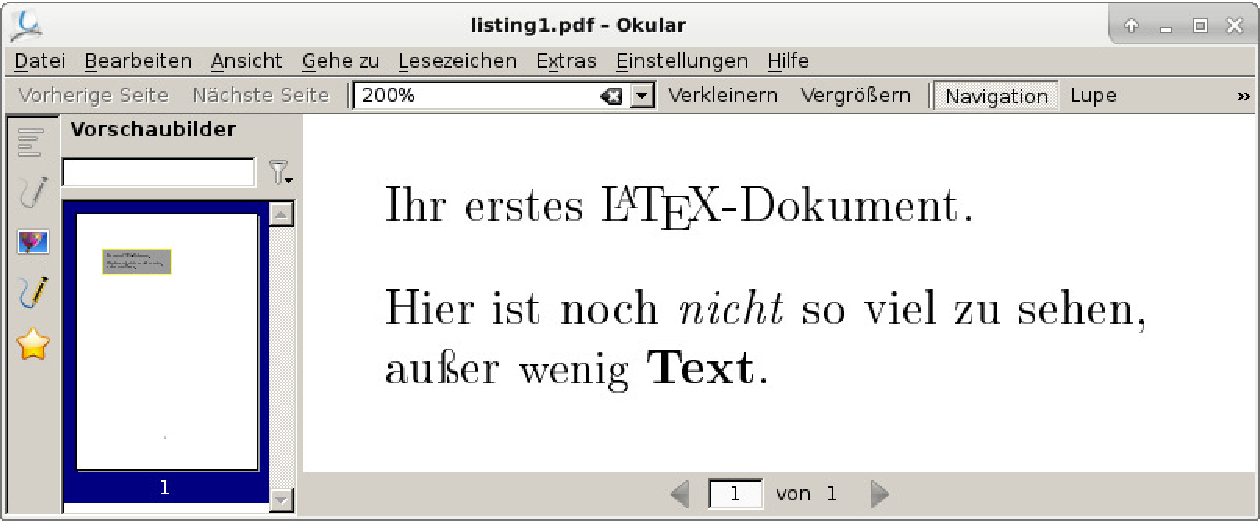
\includegraphics[width=\textwidth]{Screenshot_Listing_01.pdf}
% \end{center}

\begin{figure}[H]
%     \centering
         % Abschneiden mit trim = liks unten rechts oben
         \fbox{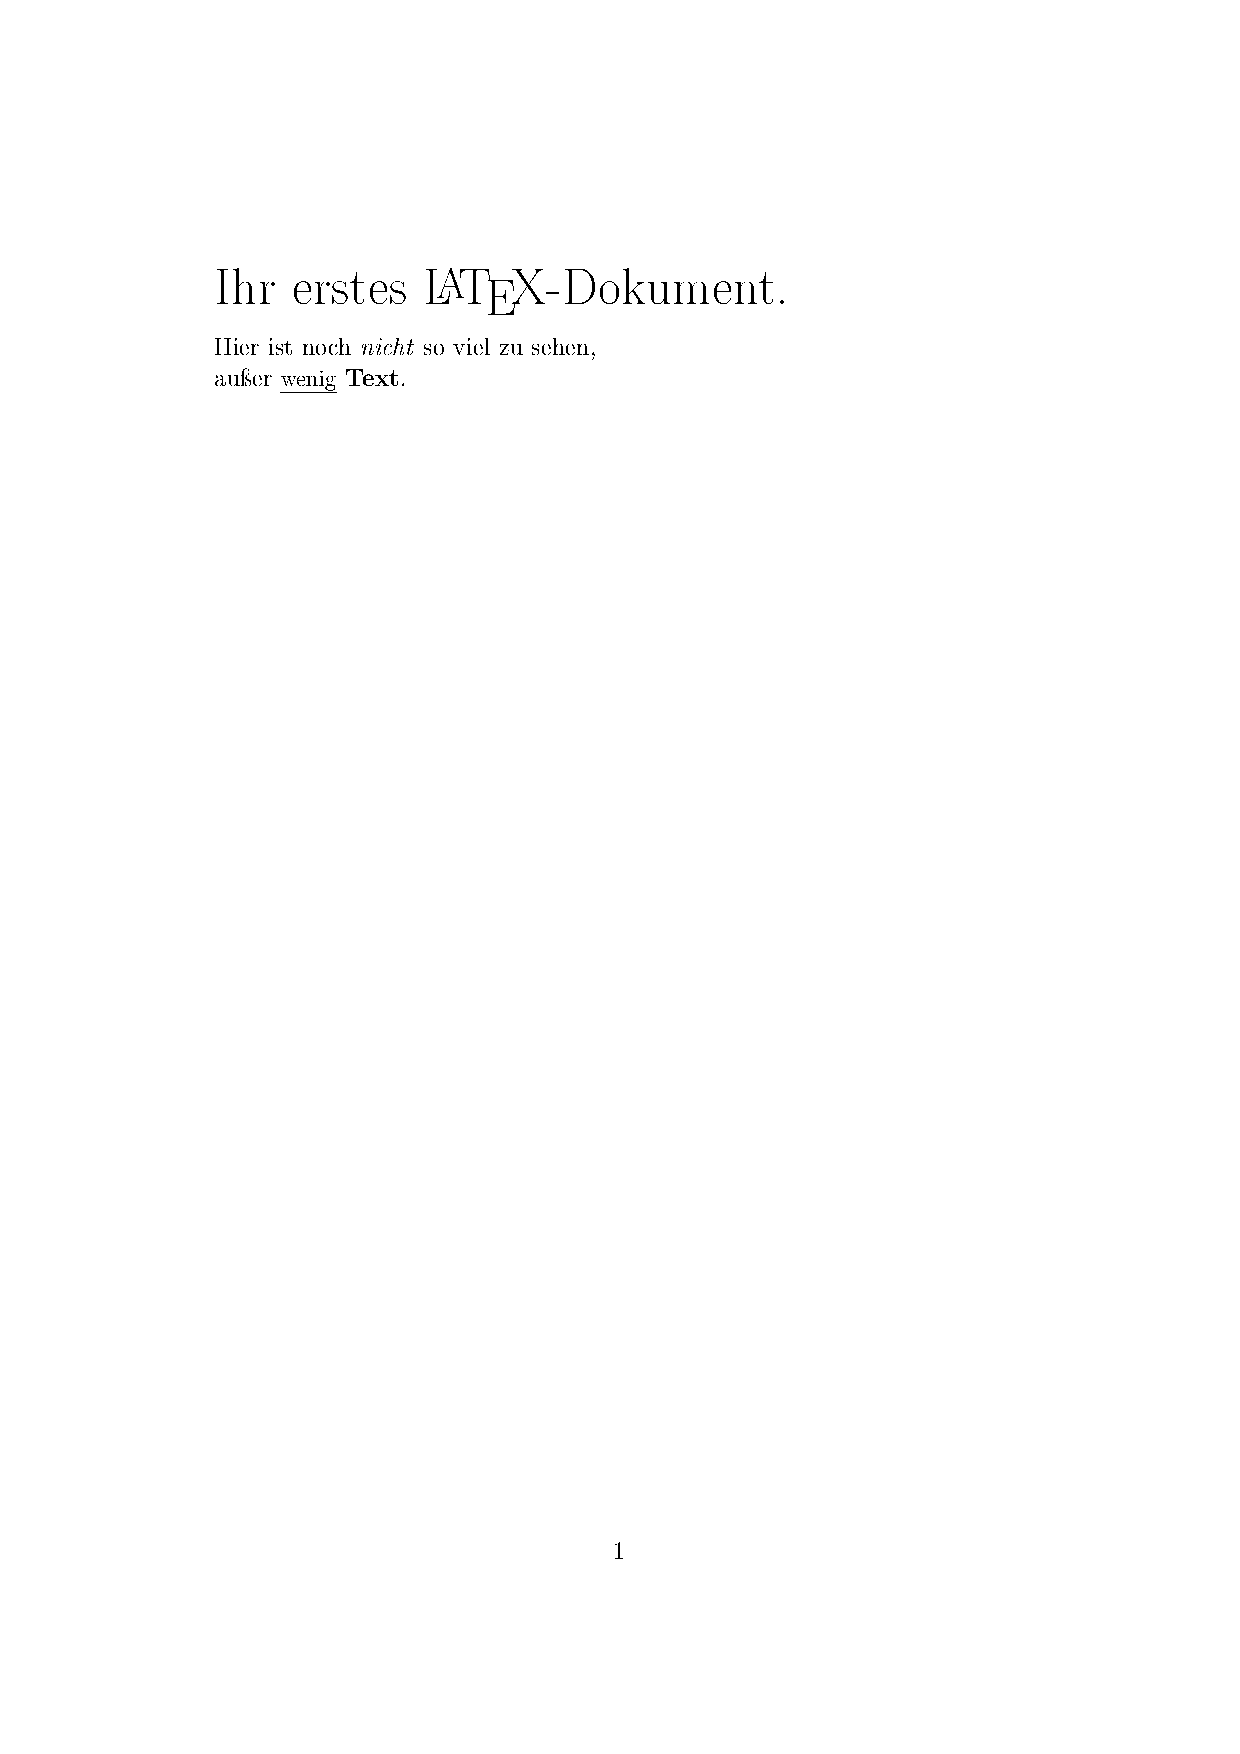
\includegraphics[page=1, clip, trim=3cm 22.5cm 3cm 4cm,  width=.98\textwidth]{Beispiele/Listing_01/listing1.pdf}}
    \caption{Resultat von Listing~\ref{erstesbeispiel}}
    \label{fig_Listing1}
\end{figure}


\chapter{Befehle, Gruppen, Umgebungen und Zeichen}
\label{BefehleGruppenUmgebungenZeichenKapitel}

In diesem Kapitel erfahren Sie, was in der Auszeichnungssprache von \LaTeX\ Befehle und Umgebungen sind, und wie Sie mit diesen arbeiten können. Zudem enthält dieses Kapitel einige wichtige Sonderzeichen und präsentiert eine Auswahl grundlegender Befehle und Umgebungen anhand von Beispielen.

\section{Befehle}
\index{Befehle}

Wie auf Seite~\pageref{Seite_Befehl} beschrieben, leitet der Backslash (\verb!\!), der sogenannte \emph{Escape Character} LaTeX-Befehle ein. Befehle können mehrere Argumente haben. Zwingende Argumente\index{Argument!zwingend} stehen meist in geschweiften\index{Klammern!geschweift} Klammern \verb!{...}!, in manchen Fällen
auch in runden\index{Klammern!rund} \verb!(...)!. Optionale Argumente sind in eckigen\index{Klammern!eckig} Klammern \verb![...]! angegeben.

\fbox{\texttt{\textbackslash}\textsl{befehl}\texttt{[}\textsl{optionale Argumente}\texttt{]}\texttt{\{}\textsl{zwingende Argumente}\texttt{\}}}

In den allermeisten Fällen Befehle mit Kleinbuchstaben geschrieben. Dabei ist zu beachten, dass \LaTeX\ \emph{case sensitive} arbeitet. Es unterscheidet also bei den Namen von Befehlen zwischen Groß- und Kleinschreibung. Zudem dürfen die Namen von Befehlen nur Buchstaben enthalten. 

Jede Zeile kann mehrere Befehle enthalten und die Reichweite eines Befehls beginnt ab der Stelle im Quelltext, wo er auftritt, bis zum Ende der lokalen Gruppe.


\section{Gruppen}
\index{Gruppe}

Eine Gruppe ist ein Textbereich, der von geschweiften Klammern eingeschlossen ist. Der Inhalt 
einer Gruppe beginnt also nach \verb!{! und reicht bis zur nächsten  schließenden geschweiften Klammer \verb!}!.

Gruppen werden häufig verwendet, um einen Textabschnitt in einer anderen Schriftart oder Schriftgröße zu setzen. Dafür wird vor den Text der Gruppe der gewünschte Befehl geschrieben. Dieser Befehl hat dann auch nur innerhalb der geschweiften Klammern Gültigkeit. Einige Beispiele für Gruppen enthält Listing~\ref{zweitesbeispiel}. Das Ergebnis dieses Beispiels zeigt Abbildung~\ref{fig_Listing2}.

\lstinputlisting[caption={Ein Beispiel zu Gruppen},label=zweitesbeispiel, style=customlatex]{Beispiele/Gruppen/gruppen.tex}

\begin{figure}[H]
%     \centering
         % Abschneiden mit trim = liks unten rechts oben
         \fbox{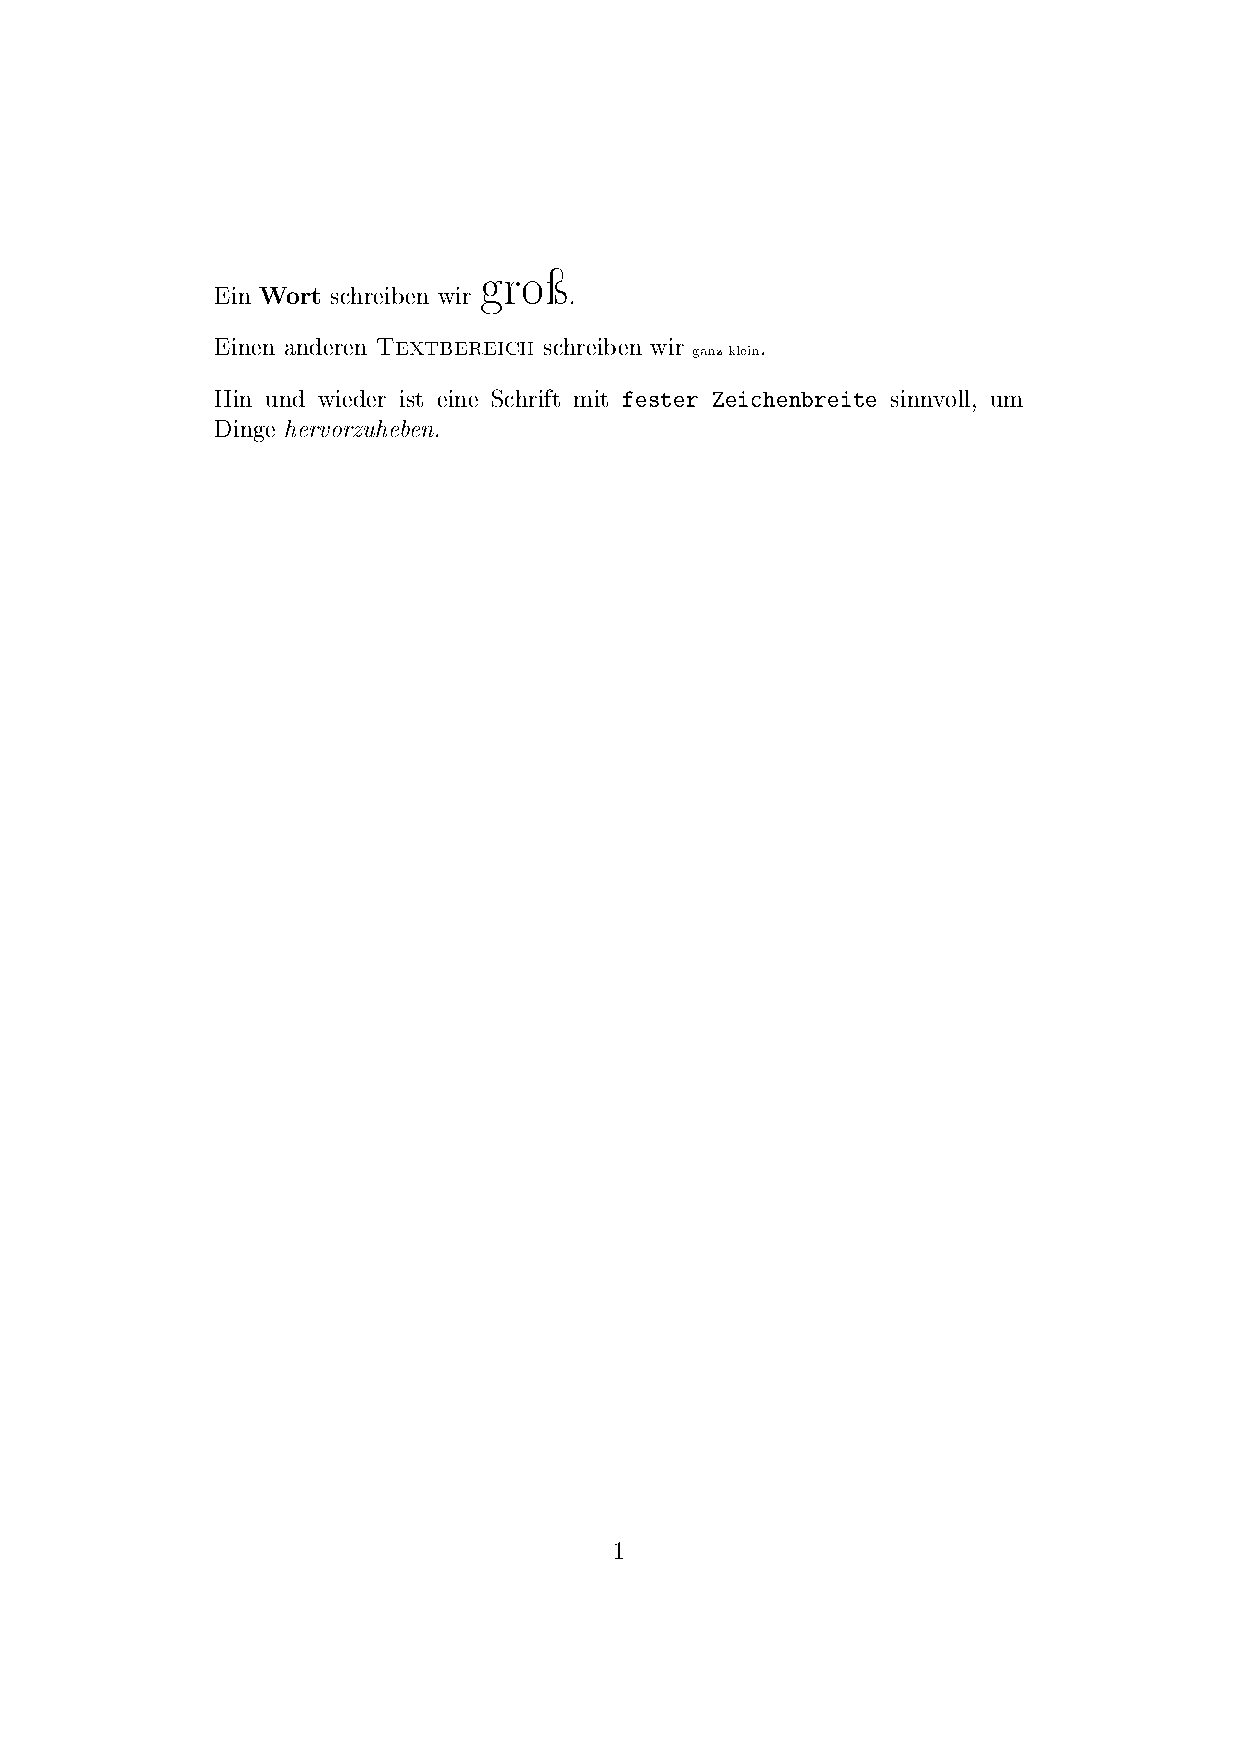
\includegraphics[page=1, clip, trim=3cm 21.5cm 3cm 4cm, width=.98\textwidth]{Beispiele/Gruppen/gruppen.pdf}}
    \caption{Resultat von Listing~\ref{zweitesbeispiel}}
    \label{fig_Listing2}
\end{figure}


\section{Umgebungen}
\index{Umgebung}

Umgebungen beginnen mit dem Befehl \verb!\begin{!\textsl{Umgebung}\verb!}!
und enden mit dem Befehl \verb!\end{!\textsl{Umgebung}\verb!}!.

Zwischen dem Anfang und dem Ende einer Umgebung können Texte und auch
Befehle stehen. Allerdings sind nicht alle Befehle innerhalb aller
Umgebungen zulässig. Ein Beispiel dafür ist der Befehl \verb!\verb! zum
Satz unformatierter Texte mit fester Zeichenbreite. Dessen Verwendung ist bei zahlreichen Umgebungen nicht zulässig.

Es ist auch möglich, Umgebungen miteinander zu verschalten. Das ist beispielsweise nötig, um Aufzählungen mit mehreren Ebenen (siehe Abschnitt~\ref{Abschnitt_Aufzaehlungen}) zu realisieren.



\section{Maßangaben mit absoluten und relativen Maßeinheiten}
\index{Massangaben}
\index{Maßeinheit}

Maßeinheiten und feste\index{Maßeinheit!fest} sowie elastische\index{Maßeinheit!fest} Maße ermöglichen es, das Layout von Dokumenten zu definieren. 

Maßangaben bestehen aus mindestens einer Dezimalzahl\index{Dezimalzahl} (mit oder ohne Vorzeichen) und aus einer 
Maßeinheit, die direkt (ohne Leerzeichen) auf die Zahl folgt. Eine Übersicht über die unterstützten Maßeinheiten zeigt Tabelle~\ref{Tabelle_Masseinheiten}. Dezimalzahlen dürfen bei \LaTeX\ mit einem Komma oder alternativ mit einem Dezimalpunkt\index{Dezimalpunkt} geschrieben werden, um die Nachkommastellen kenntlich zu machen. Somit sind beispielsweise \verb!3.5cm! und 
\verb!3,5cm!, sowie \verb!3cm! erlaubte Angaben.

\LaTeX\ kennt neun absolute und zwei relative Maßeinheiten. Die relativen Maßeinheiten \verb!em! und \verb!ex! orientieren sich an der aktuell verwendeten Schriftart. 



\begin{table}[h!tb]
\centering
\caption[Absolute und relative Maßeinheiten]{Absolute und relative Maßeinheiten~\cite{Schwarz1988}}
\label{Tabelle_Masseinheiten}       % Give a unique label
\begin{tabular}{clll}
\hline
Abkürzung & Bedeutung & \multicolumn{2}{c}{Umrechnungen}  \\
\hline
\texttt{pt} & \glqq\textsl{Point}\grqq\ (Punkt) & 1\,pt = 0,013837\,in & 1\,pt = 0,0351\,cm \\
\texttt{pc} & Pica & 1\,pc = 12\,pt & 1\,pc = 0,422\,cm \\
\texttt{in} & \glqq\textsl{Inch}\grqq\ (Zoll) & 1\,in = 72,27\,pt & 1\,in = 2.54\,cm \\
\texttt{mm} & Millimeter & 1\,mm = 2,845\,pt \\
\texttt{cm} & Zentimeter & 1\,cm = 28,45\,pt & 1\,cm = 10\,mm\\
\texttt{bp} & Big Point & 72\,bp = 1\,in & 1\,bp = 0,03528\,cm\\
\texttt{dd} & Didot Punkt & 1157\,dd = 1238\,pt & 1\,dd = 0,03761\,cm\\
\texttt{cc} & Cicero & 1\,cc = 12\,dd & 1\,cc = 0,45132\,cm \\
\texttt{sp} & Scaled Point & 65536\,sp = 1\,pt & 1\,sp \(<\) 0,6 \(*\) 10\textsuperscript{-6}\,cm\\
\texttt{em} & Geviert & \multicolumn{2}{l}{Relatives Maß. Ist ca. die Breite von \glqq M\grqq} \\  
\texttt{ex} & & \multicolumn{2}{l}{Relatives Maß. Ist ca. die Höhe von \glqq x\grqq} \\ 
\hline
\end{tabular}
\end{table}
% Solche Tabellen/Gegenüberstellungen finden sich in allen Dokumentationen zu TeX/LaTeX


Das \emph{Geviert}\index{Geviert} und ist eine typografische Maßeinheit 
aus der Zeit des Bleisatzes mit beweglichen Lettern. Ein Geviert bezeichnet dabei die Schriftgröße (Kegelhöhe)\index{Kegelhöhe}. Bei einer Schriftgröße von 12\,Punkten hat ein Geviert dementsprechend eine Länge von 12\,Punkten~\cite{LeerraumGevierte_Webpage}. 

Bei der Arbeit mit \LaTeX\ kommt es häufig vor, dass Absatzeinzüge\index{Absatzeinzüge} 
in Geviert angegeben sind (meist \verb!1em! oder \verb!2em!). Auch die konkreten Längen der unterschiedlichen horizontalen Striche im Text -- Geviertstrich\index{Geviertstrich}, Halbgeviertstrich\index{Halbgeviertstrich} (Gedankenstrich)\index{Gedankenstrich} und Viertelgeviertstrich\index{Viertelgeviertstrich} (Bindestrich)\index{Bindestrich} hängen von der Seitenlänge des Gevierts und damit von der Schriftgröße ab~\cite{Geviert_Wiki_Webpage}.

Während das relative Maß \verb!em! meist für horizontalen Maße verwendet\index{Maß!horizontal} wird, eignet sich \verb!ex! besonders für vertikale Maße\index{Maß!vertikal}. 

In der Literatur zu \LaTeX\ findet sich auch immer wieder die Aussage, dass \verb!em! etwas der 
Breite des Großbuchstabens \glqq M\grqq\ und \verb!ex! in etwa der Höhe des Buchstabens \glqq x\grqq\ im aktuellen Font entspricht.~\cite{Kopka2000,Schwarz1988}


% Quellen: Schwarz1988: S.22
% Kopka2000: S.14


\subsection{Anwendungsbeispiele}

Mit den in diesem Abschnitt beschriebenen Maßeinheiten werden unter anderem 
Längenbefehlen\index{Längenbefehle}, die das Dokumentenlayout definieren, Werte zugewiesen

Um beispielsweise die Höhe und Breite des Textes festzulegen, müssen den Längenbefehlen \verb!\textheight! und \verb!\textwidth! mit dem Befehl \verb!\setlength! die gewünschten Werte zugewiesen werden.


\fbox{\texttt{\textbackslash setlength\{\textbackslash \textsl{Längenbefehl}\}\{\textsl{Maßangabe}\}}}


Soll beispielsweise ein Dokument eine Texthöhe\index{Texthöhe} von 18\,cm und eine
Textbreite\index{Textbreite} von 13,5\,cm haben, muss dieses mit den folgenden beiden Zeilen in der Präambel der \verb!.tex!-Quelldatei definiert werden.


\begin{Verbatim}[frame=single]
\setlength{\textwidth}{13.5cm}
\setlength{\textheight}{18cm}
\end{Verbatim}

Weitere häufige Anwendungsbeispiele, wo die Maßangaben eine Rolle spielen, sind Befehle um horizontale oder vertikale Abstände zu definieren, wie zum Beispiel \verb!\hspace! und \verb!\vspace!, sowie Abbildungen und Tabellen.

\subsection{Elastische Maße}
\label{Elastische_Masse}

Der Unterschied zwischen festen und elastischen 
Maßen ist, das elastische Maße um festzulegende Werte gestreckt und gestaucht werden
können. Die Definition eines elastischen Maßes erfolgt mit drei Werten~\cite{Kopka2000}: 

\begin{itemize}
\item Sollwert 
\item Streckwert -- der Wert, um den maximal gestreckt werden darf
\item Stauchwert -- der Wert, um den maximal gestaucht werden darf
\end{itemize}

Die Syntax für ein elastisches Maß ist:


\fbox{\texttt{\textbackslash setlength\{\textbackslash \textsl{Befehl}\}\{\textsl{Sollwert} plus \textsl{Streckwert} minus \textsl{Stauchwert}\}}}

Das folgende Beispiel zeigt ein Anwendungsbeispiel. Dieses definiert den Zeilenabstand zwischen Absätzen auf elastische Art und Weise.

\begin{Verbatim}[frame=single]
\setlength{\parskip}{2ex plus 0.3ex minus 0.5ex}
\end{Verbatim}

Konkret ist hier definiert, das der Abstand zwischen zwei 
Absätzen zweimal so hoch sein soll, wie der Buchstabe \glqq x\grqq\ im aktuellen Zeichensatz hoch ist. Der Abstand darf bei Bedarf bis auf den 2,3-fachen Abstand gedehnt oder auf den 1,5-fachen Abstand gestaucht werden.


\section{Sonderzeichen}

Sonderzeichen sind unter \LaTeX\ einerseits
Zeichen, die eine besondere Funktion haben (beispielsweise \verb!&! und
\verb!$!), andererseits sind Sonderzeichen aber auch Zeichen, für die auf 
einer normalen Tastatur keine Taste existiert (zum Beispiel
\copyright, \dag und \ddag).

Buchstaben mit Akzenten sind im Grunde auch so etwas wie 
Sonderzeichen und Anführungszeichen\index{Anführungszeichen} 
aller Art sowie Punkte und Striche
der verschiedensten Form kann man auch als Sonderzeichen bezeichnen.


\subsection{Besondere Zeichen}

\LaTeX\ kennt eine große Zahl besonderer Zeichen, die auch Sonderzeichen heißen. Dieser Abschnitt präsentiert eine Auswahl an vergleichsweise häufig verwendeten besonderen Zeichen. Diese sind:


\begin{center}
\textbackslash\ \quad \$ \quad \& \quad \% \quad \# \quad \_  
\quad \textasciitilde\ \quad \textasciicircum\ \quad \{ \quad \}
\end{center}


Diese besonderen Zeichen haben bei der Texteingabe eine spezielle Bedeutung (siehe Tabelle~\ref{Tabelle_Sonderzeichen}) und die meisten von ihnen können durch das Voranstellen eines Backslashs\index{Backslash} (\verb!\!) dargestellt werden.

\begin{table}[h!tb]
\centering
\caption{Besondere Zeichen}
\label{Tabelle_Sonderzeichen}       % Give a unique label
\begin{tabular}{cp{6.7cm}p{4cm}}
\hline
Zeichen & Bedeutung des Zeichens & Befehl \\
\hline
\textbackslash & Mit einem Backslash beginnt ein Befehl  & \texttt{\textbackslash textbackslash} \\
\$ & Schaltet in den Mathematikmodus um & \texttt{\textbackslash \$} \\
\& & Markiert die Grenzen der Tabellenspalten & \texttt{\textbackslash \&} \\
\% & Alles bis zum Zeilenende wird ignoriert & \texttt{\textbackslash \%} \\
\# & Makroparameterzeichen & \texttt{\textbackslash \#} \\ 
\_ & Definiert im Mathematikmodus Indizes & \texttt{\textbackslash textunderscore} oder \texttt{\textbackslash \_} \\
\textasciitilde & Fügt einen untrennbaren Zwischenraum ein & \texttt{\textbackslash textasciitilde} \\
\textasciicircum & Definiert im Mathematikmodus Exponenten 
 & \texttt{\textbackslash textasciicircum} \\
\{ & Definiert den Anfang einer Gruppe & \texttt{\textbackslash\{} \\
\} & Definiert das Ende einer Gruppe &  \texttt{\textbackslash\}} \\
\hline
\end{tabular}
\end{table}



\subsection{Einige häufig verwendete Zeichen bzw. Symbole}

\LaTeX\ bietet eine große Anzahl von Zeichen, die auch Symbole heißen. Tabelle~\ref{Tabelle_Symbole} präsentiert einige der häufiger verwendeten.


\begin{table}[h!tb]
\centering
\caption{Zeichen (Symbole)}
\label{Tabelle_Symbole}       % Give a unique label
\begin{tabular}{cll}
\hline
Symbol & Bezeichnung & Schreibweise \\ 
\hline
\copyright & Copyright\index{Copyright} & \texttt{\textbackslash copyright} \\
\textregistered & Registered\index{Registered-Zeichen} & \texttt{\textbackslash textregistered} \\
\texttrademark & Trademark\index{Trademark-Zeichen} & \texttt{\textbackslash texttrademark} \\
\S & Juristischer Paragraph & \texttt{\textbackslash S}\\
\P & Paragraph\index{Paragraph-Zeichen} & \texttt{\textbackslash P}\\
\euro & Euro\index{Euro} & \texttt{\textbackslash euro} \\
\pounds & Pfund Sterling\index{Pfund Sterling} & \texttt{\textbackslash pounds} \\
\textyen & Yen\index{Yen} & \texttt{\textbackslash textyen} \\
\dag & Dagger\index{Dagger-Zeichen} & \texttt{\textbackslash dag} \\
\ddag & Doppel-Dagger\index{Doppel-Dagger-Zeichen} & \texttt{\textbackslash ddag} \\ 
\textbullet & Aufzählungspunkt\index{Aufzählungspunkt} & \texttt{\textbackslash textbullet} \\
@ & Klammeraffe & \texttt{@} \\
\hline
\end{tabular}
\end{table}

Auch für die in diesem Dokument schon mehrfach verwendeten Schriftzüge von \TeX\ und \LaTeX\ gibt es entsprechende Befehle. Diese enthält Tabelle~\ref{Tabelle_Schriftzuege}.

\begin{table}[h!tb]
\centering
\caption{Befehle zum komfortablen Satz der \TeX/\LaTeX-Schriftzüge}
\label{Tabelle_Schriftzuege}       % Give a unique label
\begin{tabular}{cll}
\hline
Symbol & Bezeichnung & Befehl \\ 
\hline
\TeX & Schriftzug von \TeX & \texttt{\textbackslash TeX} \\
\LaTeX & Schriftzug von \LaTeX & \texttt{\textbackslash LaTeX} \\
\LaTeXe & Schriftzug der seit 1994 aktuellen Version von \LaTeX & \texttt{\textbackslash LaTeXe} \\
\hline
\end{tabular}
\end{table}


Eine sehr große Zahl weiter Zeichen enthält das Erweiterungspaket \verb!textcomp.sty!, das mit dem Befehl \verb!\usepackage{textcomp}! in der Präambel eines \LaTeX-Quelltextes eingebunden. Eine Auswahl der Befehle im Paket \verb!textcomp! enthält Tabelle~\ref{Tabelle_SymboleTextcomp}.



% \begin{table}[h!tb]
% \centering
\begin{longtable}{lclc}
\caption{Zeichen aus dem Erweiterungspaket \texttt{textcomp}}
\label{Tabelle_SymboleTextcomp}       % Give a unique label
\endfirsthead
\endhead
\hline
Befehl  & Zeichen &  Befehl & Zeichen  \\  
\hline
\texttt{\textbackslash textdollaroldstyle} & \textdollaroldstyle &
\texttt{\textbackslash textcentoldstyle} & \textcentoldstyle \\
\texttt{\textbackslash textdollar} & \textdollar &
\texttt{\textbackslash textcent} & \textcent \\[1em]
\texttt{\textbackslash textzerooldstyle} & \textzerooldstyle &
\texttt{\textbackslash textoneoldstyle} & \textoneoldstyle \\
\texttt{\textbackslash texttwooldstyle} & \texttwooldstyle &
\texttt{\textbackslash textthreeoldstyle} & \textthreeoldstyle \\
\texttt{\textbackslash textfouroldstyle} & \textfouroldstyle &
\texttt{\textbackslash textfiveoldstyle} & \textfiveoldstyle \\
\texttt{\textbackslash textsixoldstyle} & \textsixoldstyle &
\texttt{\textbackslash textsevenoldstyle} & \textsevenoldstyle \\
\texttt{\textbackslash texteightoldstyle} & \texteightoldstyle &
\texttt{\textbackslash textnineoldstyle} & \textnineoldstyle \\[1em]
\texttt{\textbackslash texttimes} & \texttimes &
\texttt{\textbackslash textonesuperior} & \textonesuperior \\
\texttt{\textbackslash texttwosuperior} & \texttwosuperior &
\texttt{\textbackslash textthreesuperior} & \textthreesuperior \\
\texttt{\textbackslash textonequarter} & \textonequarter &
\texttt{\textbackslash textonehalf} & \textonehalf \\
\texttt{\textbackslash textthreequarters} & \textthreequarters &
\texttt{\textbackslash textsurd} & \textsurd \\
\texttt{\textbackslash textperthousand} & \textperthousand & & \\[1em]
\texttt{\textbackslash textrightarrow} & \textrightarrow &
\texttt{\textbackslash textleftarrow} & \textleftarrow \\
\texttt{\textbackslash textuparrow} & \textuparrow &
\texttt{\textbackslash textdownarrow} & \textdownarrow \\[1em]
\texttt{\textbackslash textdagger} & \textdagger &
\texttt{\textbackslash textdaggerdbl} & \textdaggerdbl \\
\texttt{\textbackslash textohm} & \textohm &
\texttt{\textbackslash textmho} & \textmho \\
\texttt{\textbackslash textlbrackdbl} & \textlbrackdbl &
\texttt{\textbackslash textrbrackdbl} & \textrbrackdbl \\[1em]
\texttt{\textbackslash textcopyright} & \textcopyright &
\texttt{\textbackslash textcopyleft} & \textcopyleft \\
\texttt{\textbackslash textregistered} & \textregistered &
\texttt{\textbackslash textcircledP} & \textcircledP \\
\texttt{\textbackslash texttrademark} & \texttrademark &
\texttt{\textbackslash textservicemark} & \textservicemark \\
\texttt{\textbackslash textnumero} & \textnumero &
\texttt{\textbackslash textestimated} & \textestimated \\[1em]
\texttt{\textbackslash textdegree} & \textdegree &
\texttt{\textbackslash textcelsius} & \textcelsius \\
\texttt{\textbackslash textbullet} & \textbullet &
\texttt{\textbackslash textopenbullet} & \textopenbullet \\
\texttt{\textbackslash textasteriskcentered} & \textasteriskcentered &
\texttt{\textbackslash textmusicalnote} & \textmusicalnote \\
\texttt{\textbackslash textordfeminine} & \textordfeminine &
\texttt{\textbackslash textordmasculine} & \textordmasculine\\
\texttt{\textbackslash textlquill} & \textlquill &
\texttt{\textbackslash textrquill} & \textrquill \\
\texttt{\textbackslash textbardbl} & \textbardbl &
\texttt{\textbackslash textbrokenbar} & \textbrokenbar \\[1em]
\texttt{\textbackslash textthreequartersemdash} & \textthreequartersemdash &
\texttt{\textbackslash texttwelveudash} & \texttwelveudash \\
\texttt{\textbackslash texttimes} & \texttimes &
\texttt{\textbackslash textdiv} & \textdiv \\
\texttt{\textbackslash textminus} & \textminus &
\texttt{\textbackslash textdblhyphen} & \textdblhyphen \\
\texttt{\textbackslash textdiscount} & \textdiscount &
\texttt{\textbackslash textfractionsolidus} & \textfractionsolidus \\
\texttt{\textbackslash textlangle} & \textlangle &
\texttt{\textbackslash textrangle} & \textrangle \\[1em]
\texttt{\textbackslash textparagraph} & \textparagraph &
\texttt{\textbackslash textpilcrow} & \textpilcrow \\
\texttt{\textbackslash textreferencemark} & \textreferencemark &
\texttt{\textbackslash textcurrency} & \textcurrency \\
\texttt{\textbackslash textsection} & \textsection &
\texttt{\textbackslash textbigcircle} & \textbigcircle \\[1em]
\texttt{\textbackslash textquotestraightdblbase} & \textquotestraightdblbase &
\texttt{\textbackslash textquotestraightbase} & \textquotestraightbase \\
\texttt{\textbackslash textquotesingle} & \textquotesingle &
\texttt{\textbackslash texttildelow} & \texttildelow \\
\texttt{\textbackslash textasciibreve} & \textasciibreve &
\texttt{\textbackslash textasciicaron} & \textasciicaron \\
\texttt{\textbackslash textperiodcentered} & \textperiodcentered &
\texttt{\textbackslash textasciidieresis} & \textasciidieresis \\
\texttt{\textbackslash textlnot} & \textlnot &
\texttt{\textbackslash textdblhyphenchar} & \textdblhyphenchar \\
\texttt{\textbackslash textpm} & \textpm &
\texttt{\textbackslash textasciimacron} & \textasciimacron \\
\texttt{\textbackslash textgravedbl} & \textgravedbl &
\texttt{\textbackslash textacutedbl} & \textacutedbl \\
\texttt{\textbackslash textasciigrave} & \textasciigrave &
\texttt{\textbackslash textasciiacute} & \textasciiacute \\
\hline
\end{longtable}
% \end{table}


% \par
% \begin{tabularx}{\textwidth}{>{\setlength{\hsize}{1.3\hsize}}X%
% >{\setlength{\hsize}{.7\hsize}}Y>{\setlength{\hsize}{1.3\hsize}}X%
% >{\setlength{\hsize}{.7\hsize}}Y}
% \texttt{\textbackslash textquotestraightdblbase} & \textquotestraightdblbase &
% \texttt{\textbackslash textquotestraigh!tbase} & \textquotestraigh!tbase \\
% \texttt{\textbackslash textquotesingle} & \textquotesingle &
% \texttt{\textbackslash texttildelow} & \texttildelow \\
% \texttt{\textbackslash textasciibreve} & \textasciibreve &
% \texttt{\textbackslash textasciicaron} & \textasciicaron \\
% \texttt{\textbackslash textperiodcentered} & \textperiodcentered &
% \texttt{\textbackslash textasciidieresis} & \textasciidieresis \\
% \texttt{\textbackslash textlnot} & \textlnot &
% \texttt{\textbackslash textdblhyphenchar} & \textdblhyphenchar \\
% \texttt{\textbackslash textpm} & \textpm &
% \texttt{\textbackslash textasciimacron} & \textasciimacron \\
% \texttt{\textbackslash textgravedbl} & \textgravedbl &
% \texttt{\textbackslash textacutedbl} & \textacutedbl \\
% \texttt{\textbackslash textasciigrave} & \textasciigrave &
% \texttt{\textbackslash textasciiacute} & \textasciiacute \\
% \end{tabularx}
% \begin{tabularx}{\textwidth}{Y}
% \rowcolor[gray]{0.9}
% \textsl{Tabelle 5.6: Auswahl an Zeichen aus dem \texttt{textcomp}-Paket}
% \end{tabularx}


\subsection{Punkte und Striche}

Tabelle~\ref{Tabelle_Horizontale_Striche} zeigt eine Übersicht über die Befehle von \LaTeX, um unterschiedliche Arten von horizontalen Strichen zu setzen. 

\begin{table}[h!tb]
	\centering
	\caption{Horizontale Striche}
	\label{Tabelle_Horizontale_Striche}       % Give a unique label
	\begin{tabular}{cll}
		\hline
		Symbol & Bezeichnung & Befehl \\ 
		\hline
		- & Trenn-/Bindestrich & \texttt{-} oder \texttt{\textbackslash texthyphenchar}\\
		-- & Gedankenstrich & \texttt{-{}-} oder \texttt{\textbackslash textendash} \\
		--- & längerer Gedankenstrich & \texttt{-{}-{}-} oder \texttt{\textbackslash textemdash} \\
		\hline
	\end{tabular}
\end{table}

Der Trennstich\index{Trennstich} (-), der auch Viertelgeviertstrich\index{Viertelgeviertstrich} heißt, wird als Trennzeichen beim Trennen von Wörtern, oder als \textsl{Bindestrich}\index{Bindestrich} in zusammengesetzten Begriffen benutzt. Er wird wie ein ganz gewöhnlicher horizontaler Strich (\texttt{-}) geschrieben.

Der Gedankenstrich\index{Gedankenstrich} (--), der auch Halbgeviertstrich\index{Halbgeviertstrich} heißt, wird oft bei Strecken- oder Zeitangaben benutzt. Er wird mit zwei Strichen (\texttt{-{}-}) oder alternativ mit dem Befehl \verb!\textendash! erzeugt.

Primär im englischen Sprachraum wird in Dokumenten ein längerer 
Gedankenstrich (---), der sogenannte Geviertstrich\index{Geviertstrich}, verwendet. Dieser wird mit drei Strichen (\texttt{-{}-{}-}) oder dem Befehl \verb!\textemdash! erzeugt. 

\begin{table}[h!tb]
	\centering
	\caption{Fortsetzungspunkte mit \LaTeX}
	\label{Tabelle_Horizontale_Punkte}       % Give a unique label
	\begin{tabular}{cll}
		\hline
		Symbol & Bezeichnung & Befehl \\ 
		\hline
		. & gewöhnlicher Punkt & \texttt{.} \\
		... & drei gewöhnliche Punkte & \texttt{...} \\
		\dots & Fortsetzungspunkte & \texttt{\textbackslash dots}  \\
		\hline
	\end{tabular}
\end{table}


Auf den ersten Blick erscheint es kurios, das \LaTeX\ mit \verb!\dots! einen Befehl bietet, um drei aufeinander folgende Punkte, so genannte Fortsetzungspunkte\index{Fortsetzungspunkte}, zu setzen. Der Grund, warum dieser Befehl sehr sinnvoll ist, ist der Abstand zwischen den Fortsetzungspunkten. Schreibt ein Autor einfach drei Punkte hintereinander, ist der Abstand zwischen den Punkten recht klein. Der Befehl \verb!\dots! erzeugt ein optisch besseres Ergebnis. Tabelle~\ref{Tabelle_Horizontale_Punkte} zeigt den Unterschied. 



\subsection{Anführungszeichen}

\LaTeX\ ermöglicht den Satz verschiedener Anführungszeichen. Eine Übersicht präsentiert Tabelle~\ref{Tabelle_Anfuehrungszeichen}. 

\begin{table}[h!tb]
\centering
\caption{Anführungszeichen}
\label{Tabelle_Anfuehrungszeichen}       % Give a unique label
\begin{tabular}{lll}
\hline
Anführungszeichen & Kurzform & Befehl \\
\hline
\dq Doublequotes\dq & \texttt{\textbackslash dq} & \texttt{\textbackslash dq} oder \texttt{\textbackslash doublequotedbl} \\
\glqq deutsche Anführungszeichen\grqq & \texttt{\dq `}& \texttt{\textbackslash glqq} oder \texttt{\textbackslash quotedblbase} \\
& \texttt{\dq '} & \texttt{\textbackslash grqq} oder \texttt{\textbackslash quotedbrbase} \\
\glq Halbe deutsche\grq  & & \texttt{\textbackslash glq} oder \texttt{\textbackslash quotedsinglbase}\\
& & \texttt{\textbackslash grq} oder \texttt{\textbackslash quotedsingrbase}\\
\frqq französische\flqq 
 & \texttt{\dq>} & \texttt{\textbackslash frqq} oder \texttt{\textbackslash guillemontright}\\
 & \texttt{\dq<} & \texttt{\textbackslash flqq} oder \texttt{\textbackslash guillemontleft}\\
\frq Halbe französische\flq 
& & \texttt{\textbackslash frq} oder \texttt{\textbackslash guilemontright}\\
& & \texttt{\textbackslash flq} oder \texttt{\textbackslash guilemontleft}\\
\textquotedblleft anglikanische\textquotedblright & \texttt{`{}`} & \texttt{\textbackslash textquotedblleft}\\
& \texttt{'{}'} & \texttt{\textbackslash textquotedblright}\\
\textquoteleft halbe anglikanische\textquoteright & \texttt{`} & \texttt{\textbackslash textquoteleft}\\
& \texttt{'} & \texttt{\textbackslash textquoteright}\\
\hline
\end{tabular}
\end{table}

\verb!glq! steht übrigens für \textsl{german--left--quote} (deutsches 
linkes Anführungszeichen) und \verb!grq! steht für \textsl{german--right--quote} (deutsches 
rechtes Anführungszeichen).


\subsection{Akzente}

\LaTeX\ ermöglicht den Satz verschiedener Akzente (siehe Tabelle~\ref{Tabelle_Akzente}). 

\begin{table}[h!tb]
\centering
\caption{Akzente}
\label{Tabelle_Akzente}       % Give a unique label
\begin{tabular}{clclcl}
\hline
Akzent & Eingabe & Akzent & Eingabe & Akzent & Eingabe\\
\hline
\`o & \texttt{\textbackslash \textquoteleft o} & \.o & \texttt{\textbackslash .o} & \H{o} & \texttt{\textbackslash H\{o\}} \\
\'o & \texttt{\textbackslash \textquoteright o} & \u{o} & \texttt{\textbackslash u\{o\}} & \c{o} & \texttt{\textbackslash c\{o\}} \\
\^o & \texttt{\textbackslash \textasciicircum o} & \v{o} & \texttt{\textbackslash v\{o\}} & \r{o} & \texttt{\textbackslash r\{o\}} \\
\~o & \texttt{\textbackslash \textasciitilde o} & \d{o} & \texttt{\textbackslash d\{o\}} & \t{oo} & \texttt{\textbackslash t\{oo\}} \\
\=o & \texttt{\textbackslash =o} & \b{o} & \texttt{\textbackslash b\{o\}} & \textcircled{o} & \texttt{\textbackslash textcircled\{o\}} \\
\hline
\end{tabular}
\end{table}

Zudem ermöglicht \LaTeX\ den Satz mehrerer Spezialzeichen\index{Spezialzeichen}, 
wie sie in einigen europäischen 
Sprachen gängig sind. Eine Übersicht enthält Tabelle~\ref{Tabelle_Spezialzeichen}. 

\begin{table}[h!tb]
\centering
\caption{Spezialzeichen verschiedener europäischer Sprachen}
\label{Tabelle_Spezialzeichen}       % Give a unique label
\begin{tabular}{lll}
\hline
Ausgabe & Bezeichnung & Eingabe \\
\hline
\oe, \OE & Französische Ligatur & \texttt{\textbackslash oe, \textbackslash OE}\\
\ae, \AE & Lateinische, skandinavische Ligatur & \texttt{\textbackslash ae, \textbackslash AE} \\
\aa, \AA & Skandinavisches A mit Kreis & \texttt{\textbackslash aa, \textbackslash AA}\\
\o, \O & Skandinavisches O mit Strich & \texttt{\textbackslash o, \textbackslash O}\\   
\l, \L & Polnisches L mit Strich & \texttt{\textbackslash l, \textbackslash L}\\
\ss & Deutsches Es-Zet & \texttt{\textbackslash ss}\\
\hline
\end{tabular}
\end{table}


\subsection{Ligaturen}
\index{Ligatur}

Eine Ligatur ist eine Verbindung von zwei oder drei Buchstaben zu einem 
einzigen Zeichen. Anders ausgedrückt, sind Ligaturen zu einem einzelnen Zeichen zusammengerückte Buchstaben (siehe Tabelle~\ref{Tabelle_Ligaturen}). Im Einzelnen handelt es sich dabei um die Buchstabenkombinationen \verb!ff!,
\verb!fi!, \verb!fl!, \verb!ffi! und \verb!ffl!. Diese 
werden von \LaTeX\ wie folgt gesetzt: ff, fi, fl, ffi, ffl.

Streng genommen sind auch auch der Gedankenstrich und der verlängerte 
Gedankenstrich (siehe Seite~\pageref{Tabelle_Horizontale_Striche}) Ligaturen, da Sie aus zwei bzw. drei einzelnen 
Zeichen zu einem zusammengefasst werden.


\begin{table}[h!tb]
\centering
\caption{Ligaturen}
\label{Tabelle_Ligaturen}       % Give a unique label
\begin{tabular}{ccc}
\hline
Buchstabenkombination & Ligatur & unterdrückte Ligatur \\
\hline
\texttt{ff} & ff & f{}f \\
\texttt{fi} & fi & f{}i \\
\texttt{fl} & fl & f{}l \\
\texttt{ffi} & ffi & f{}f{}i \\
\texttt{ffl} & ffl & f{}f{}l \\
\hline
\end{tabular}
\end{table}

Wenn \LaTeX\ eine der vorgestellten 
Buchstabenkombinationen nicht automatisch als Ligatur setzen soll, muss der Autor dieses im Dokument unterdrücken. Anwendungsbeispiele, wo es sinnvoll sein kann, eine Ligatur zu unterdrücken, ist wenn Wörter falsch getrennt werden. 

Eine Ligatur kann unterdrückt werden, indem zwischen jedes Buchstabenpaar, das zur möglichen Ligatur gehören, ein Paar geschweifter Klammern gesetzt wird. So wird aus 
\verb!f{}f{}l! dann f{}f{}l und nicht ffl.  
Eine alternative Möglichkeit ist, zwischen jedes Buchstabenpaar, das zur möglichen
Ligatur gehört, einen Backslash und einen Slash zu setzen \verb!\/!.


\chapter{Dokumentklassen und Seitenstile}
\label{KapitelDokumentklassenSeitenstile}

Die in diesem Kapitel beschriebenen Dokumentklassen und Seitenstile definieren die grundlegenden Parameter des Layouts eines Dokuments. Zudem präsentiert dieses Kapitel die benötigten Befehle und Umgebungen, um Dokumente sinnvoll zu gliedern. 

\section{Dokumentklassen}
\label{AbschnittDokumentklassen}
\index{Dokumentklasse}

Der erste Befehl, der in der Präambel einer \LaTeX-Quelldatei (\verb!.tex!-Datei) steht, ist der Befehl \verb!\documentclass!
\index[cmd]{\texttt{\textbackslash documentclass}}. Dieser definiert im Parameter \verb!Dokumentklasse!
die Dokumentklasse für das gesamte Dokument. 

\fbox{\texttt{\textbackslash documentclass[}\textsl{Optionen}\texttt{]\{}\textsl{Dokumentklasse}\texttt{\}}}

Mehr als eine Dokumentklasse pro Dokument ist unzulässig. Moderne \LaTeX-Distributionen bringen eine große Anzahl an Dokumentklassen mit. Weil dieses Dokument aus Platzgründen nicht alle beschreiben kann, liegt an dieser Stelle der Fokus auf denjenigen Dokumentklassen, die seit Jahrzehnten sehr populär sind, und die in der Literatur und in der Praxis häufig eingesetzt werden. Zusätzlich berücksichtigt diese Dokumentation einige der neueren KOMA-Klassen~\cite{KOMAScript_Dokumentation}, die sich speziell den Gepflogenheiten des deutschen Sprachraums widmen. 

Im Detail handelt es sich bei den hier vorgestellten traditionellen Dokumentklassen um 
\verb!article!\index[cmd]{\texttt{article}}, 
\verb!book!\index[cmd]{\texttt{book}}, 
\verb!proc!\index[cmd]{\texttt{proc}}, 
\verb!report!\index[cmd]{\texttt{report}}, 
\verb!letter!\index[cmd]{\texttt{letter}}
und \verb!slides!\index[cmd]{\texttt{slides}}. 



Die Dokumentklasse 
\verb!article! eignet sich gut für kleinere bis mittelgroße Dokumente. Texte, die mit dieser Dokumentklasse realisiert werden, können in
Abschnitte (\textsl{Sections}), Unterabschnitte (\textsl{Subsections}) usw. untergliedert werden. Kapitel (\textsl{Chapter}) kennt diese Klasse aber leider nicht.

Für längere Texte, die in Kapitel, Abschnitte, Unterabschnitte usw. unterteilen werden sollen, eignet sich u.a. die Dokumentklasse \verb!report!.
Für Bücher oder sonstige umfangreiche Dokumente, die in Kapitel,
Abschnitte und Unterabschnitte untergliedert sein sollen, eignet sich die Dokumentklasse \verb!book!. Bei den Dokumentklassen \verb!book! und \verb!report! beginnen Kapitel auch immer mit einer neuen Seite.

Speziell zur Erstellung von Sitzungsprotokollen eignet sich die Dokumentklasse \verb!proc!.

Die Dokumentklasse \verb!letter! ist eine auf US-amerikanische 
Briefe zugeschnittene Klasse. Für Briefe nach deutschem Standard sind 
andere Klassen wie \verb!dinbrief!\index[cmd]{\texttt{dinbrief}},
\verb!g-brief! oder das modernere \verb!g-brief2!\index[cmd]{\texttt{g-brief2}} besser geeignet (siehe Kapitel~\ref{Kapitel_Briefe}). 


Die Dokumentklasse \verb!slides! eignet sich für Präsentationsfolien. Eine modernere Alternative ist \verb!beamer!\index[cmd]{\texttt{beamer}} (siehe Kapitel~\ref{Kapitel_Praesentationsfolien}).


Bei den moderneren KOMA-Dokumentklassen handelt es sich 
um \verb!scrartcl!\index[cmd]{\texttt{scrartcl}} (als Ersatz für \verb!article!),  
\verb!scrreprt!\index[cmd]{\texttt{scrreprt}} (als Ersatz für \verb!report!), 
\verb!scrbook!\index[cmd]{\texttt{scrbook}} (als Ersatz für \verb!book!) und 
\verb!scrlttr2!\index[cmd]{\texttt{scrlttr2}} (als Ersatz für \verb!letter!).






\subsection{Klassenoptionen}
\index{Klassenoptionen}

Der Befehl \verb!\documentclass! bietet die 
Möglichkeit, Optionen in 
eckigen Klammern anzugeben. 
Mit diesen wird das grundlegende Layout eines Dokuments 
angepasst. 

In den Optionen ist es unter anderem möglich, die Schriftgröße\index{Schriftgröße} der Basisschrift\index{Basisschrift} anzupassen, die Anzahl der Textspalten pro Seite und die Papiergröße sowie die Ausrichtung zu definieren.

Von den in diesem Abschnitt beschrieben Optionen muss keine zwingend angegeben werden. Sie sind optional. Sind mehrere Optionen angegeben, müssen diese mit Kommas voneinander getrennt sein, wie im folgenden Beispiel zu sehen ist:

\begin{Verbatim}[frame=single]
\documentclass[12pt,twoside,a4paper]{report}
\end{Verbatim}

\subsubsection{\texttt{10pt}, \texttt{11pt} oder \texttt{12pt}}
\index[cmd]{\texttt{10pt}}
\index[cmd]{\texttt{11pt}}
\index[cmd]{\texttt{12pt}}

Diese drei Dokumentklassenoptionen definieren die Schriftgröße\index{Schriftgröße} fest.
Ist keine der drei Alternativen angeben, wird \LaTeX\ standardmäßig die Schriftgröße \verb!10pt! wählen.

\subsubsection{\texttt{onecolumn} oder \texttt{twocolumn}}
\index[cmd]{\texttt{onecolumn}}
\index[cmd]{\texttt{twocolumn}}
\index{Seitenlayout!einspaltig}\index{Einspaltig}
\index{Seitenlayout!zweispaltig}\index{Zweispaltig}

Diese beiden Optionen ermöglichen die Definition der Seitenformatierung. 
Zur Auswahl stehen einspaltiges und zweispaltiges Seitenlayout. 
Standardmäßig verwendet \LaTeX\ ein einspaltiges Seitenlayout.

\subsubsection{\texttt{oneside} oder \texttt{twoside}}
\index[cmd]{\texttt{oneside}}
\index[cmd]{\texttt{twoside}}

Hiermit kann die Seitenformatierung auf ein- oder doppelseitige Ausgabe festgelegt werden. 

Bei doppelseitiger Ausgabe sind die linken Seitenränder von geraden und ungeraden Seiten unterschiedlich groß, so dass beim doppelseitigen Ausdruck die Textfelder 
übereinstimmen. Bei einseitiger Ausgabe sind die Seitenränder von geraden und ungeraden Seiten gleich groß.

Standardmäßig ist bei den Dokumentklassen \verb!article!, \verb!report! und \verb!letter! die einseitige Ausgabe voreingestellt. Bei der Dokumentklasse \verb!book! hingegen ist doppelseitige Ausgabe voreingestellt.

\subsubsection{\texttt{titlepage} oder \texttt{notitlepage}}
\index[cmd]{\texttt{titlepage}}
\index[cmd]{\texttt{notitlepage}}
\index{Titelseite} 

Ob eine eigene Titelseite generiert wird oder ob der Titel horizontal oben zentriert auf der ersten Dokumentseite gesetzt ist, hängt von der verwendeten Dokumentklasse ab.

Bei den Dokumentklassen \verb!book! und  \verb!report! wird eine separate Titelseite erzeugt. Bei der Dokumentklasse \verb!article! ist das nicht der Fall. Mit den Optionen \verb!titlepage! und \verb!notitlepage! können Autoren dieses Verhalten ändern. 


\subsubsection{\texttt{draft} oder \texttt{final}}
\index[cmd]{\texttt{draft}}
\index[cmd]{\texttt{final}}
\index{Zeilenumbruch} 

Bei der Option \verb!draft! werden Zeilen,
bei denen \LaTeX\ den Zeilenumbruch nicht
korrekt realisieren konnte, das heißt Zeilen, die ein wenig über den Rand des 
Textfeldes hinausragen, mit einem fetten
schwarzen Balken am Rand gekennzeichnet.
Dieser Randbalken entfällt bei der
Option \verb!final!, die die Standardeinstellung ist.


\subsubsection{\texttt{leqno}}
\index[cmd]{\texttt{leqno}}

Ist diese Dokumentklassenoption
angeben, werden die Nummern 
von mathematischen Formeln nicht 
rechtsbündig, wie sonst automatisch 
üblich, sondern linksbündig gesetzt.

\subsubsection{\texttt{fleqn}}
\index[cmd]{\texttt{fleqn}}

Mit dieser Option werden abgesetzte mathematische Formeln nicht zentriert, sondern linksbündig gesetzt.




\subsubsection{\texttt{a4paper}, \texttt{a5paper}, \texttt{b5paper}, \texttt{letterpaper}, \texttt{legalpaper} und \texttt{executivepaper}}
\index[cmd]{\texttt{a4paper}}\index{DIN-A4}
\index[cmd]{\texttt{a5paper}}\index{DIN-A5}
\index[cmd]{\texttt{b5paper}}
\index[cmd]{\texttt{letterpaper}}
\index[cmd]{\texttt{legalpaper}}
\index[cmd]{\texttt{executivepaper}}


Diese Dokumentklassenoptionen definieren die Papiergröße\index{Papiergröße}.
Standardmäßig verwendet \LaTeX\ die Option \verb!letterpaper! als 
Standard-Papierformat. Da dieses US-amerikanische Papierformat in Mitteleuropa sehr unüblich ist, sollten Autoren im europäischen Raum mit der Option \verb!a4paper! auf DIN-A4 umzustellen. Eine Übersicht über die Dimensionen der unterschiedlichen Papierformate enthält Tabelle~\ref{Tabelle_Papierformate}.

\begin{table}[h!tb]
\centering
\caption{Papierformate}
\label{Tabelle_Papierformate}       % Give a unique label
\begin{tabular}{lrclrcl}
\hline
Dokumentklassenoption & \multicolumn{3}{c}{Größe [mm]} & \multicolumn{3}{c}{Größe [Zoll]} \\
\hline
\texttt{a4paper}        & 297   & x & 210   & 11,7 & x & 8,3  \\ 
\texttt{a5paper}        & 210   & x & 148   & 8,3  & x & 5,8  \\
\texttt{b5paper}        & 250   & x & 176   & 9,8  & x & 6,9  \\ 
\texttt{letterpaper}    & 279,4 & x & 215,9 & 11   & x & 8,5  \\
\texttt{legalpaper}     & 355,6 & x & 215,9 & 14   & x & 8,5  \\
\texttt{executivepaper} & 266,7 & x & 184,1 & 10,5 & x & 7,25 \\
\hline
\end{tabular}
\end{table}


\subsubsection{\texttt{landscape}}
\index[cmd]{\texttt{landscape}}

Mit der Option \verb!landscape! wird das Dokument im Querformat gesetzt.

\subsubsection{\texttt{openright} oder \texttt{openany}}
\index[cmd]{\texttt{openright}}
\index[cmd]{\texttt{openany}}

Bei der Dokumentklasse \verb!book!
beginnt ein neues Kapitel immer 
auf einer rechten (ungeraden) Seite. Wenn ein
vorhergegangenes Kapitel auf einer 
ungeraden Seite endet, dann wird eine leere,
gerade Seite eingefügt. Mit der 
Option \verb!openany! wird dieses Verhalten
von \LaTeX\ unterdrückt. Dann kann 
ein neues Kapitel auch auf einer geraden
Seite beginnen.

Bei der Dokumentklasse \verb!report! kann ein Kapitel
standardmäßig auf jeder Seite beginnen. 
Mit der Option \verb!openright! können Autoren
festlegen, dass Kapitel (genau wie bei 
der Klasse \verb!book!) nur auf ungeraden,
rechten Seiten beginnen dürfen.

\section{Seitenstile}
\index{Seitenstil}

Der grundsätzliche Aufbau einer Seite heißt
Seitenstil. Das Festlegen des Seitenstils geschieht mit dem Befehl
\verb!\pagestyle!\index[cmd]{\texttt{\textbackslash pagestyle}} in der Präambel der \verb!.tex!-Quelldatei. 
Der gewählte Seitenstil gilt dann für das gesamte Dokument.


\fbox{\texttt{\textbackslash pagestyle\{}\textsl{Seitenstil}\texttt{\}}}

\LaTeX\ bietet
einige vorgefertigte Seitenstile (siehe Tabelle~\ref{Tabelle_Seitenstile}).
Der
Seitenstil \texttt{plain} ist die Standardauswahl von
\LaTeX, wenn kein anderer
Seitenstil mit \texttt{\textbackslash pagestyle} ausgewählt ist.

\begin{table}[h!tb]
\centering
\caption{Seitenstile}
\label{Tabelle_Seitenstile}       % Give a unique label
\begin{tabular}{lp{10.2cm}}
\hline
Seitenstil & Aussehen \\
\hline
\texttt{empty} & Die Kopf- und Fußzeilen 
bleiben leer und es wird keine
Seitennummer gesetzt. Nur das Textfeld ist zu sehen.\\
\texttt{plain} & Die Kopfzeile bleibt 
leer. In der Fußzeile wird die
Seitennummer zentriert ausgegeben.  \\
\texttt{headings} & Die Kopfzeile
jeder Seite enthält 
die aktuelle Seitenzahl und eine Überschrift. Welche Überschrift
das genau ist, hängt von der verwendeten
Dokumentklasse ab.
Für gewöhnlich handelt es sich dabei
um die aktuelle Kapitel- oder Abschnittsüberschrift. 
Die Fußzeile bleibt leer
Die einzige Ausnahme ist die jeweils 
erste Seite eines neuen Kapitels. \\
\texttt{myheadings} & Der einzige
Unterschied zum Seitenstil \texttt{headings} ist, dass die Kopfzeile nicht automatisch 
gefüllt wird, sondern das der Autor den Inhalt der Kopfzeile mit den
Befehlen \texttt{\textbackslash markright} oder
\texttt{\textbackslash markboth} festlegen muss. \\
\hline
\end{tabular}
\end{table}

Es ist auch möglich, den Seitenstil einer einzelnen Seite festzulegen. Dieses geschieht nicht in der Präambel der \verb!.tex!-Quelldatei, sondern im Text des Dokuments. Der Befehl
\verb!\thispagestyle! legt den Seitenstil der
aktuellen Seite fest -- an der Stelle im 
Quelltext, an der der Befehl auftritt.


\fbox{\texttt{\textbackslash thispagestyle\{}\textsl{Seitenstil}\texttt{\}}}


\section{Definition der Kopfzeile mit \texttt{markright} und \texttt{markboth}}
\label{markright}
\index{Kopfzeile}
\index[cmd]{\texttt{\textbackslash markright}}
\index[cmd]{\texttt{\textbackslash markboth}}

Ist ein Dokument mit den Seitenstilen \verb!headings! oder \verb!myheadings! gesetzt, können Autoren mit Hilfe der 
Befehle \verb!\markright! und \verb!markboth! die Inhalte der Kopfzeilen im Dokument definieren und damit die Standardeinstellung (siehe Tabelle~\ref{Tabelle_Standardeinstellung_Kopfzeile}) von \LaTeX\ zu überschreiben. Die
Wirkung der beiden 
Befehle \texttt{\textbackslash markright} und \texttt{\textbackslash markboth} setzt erst aber der    
zweiten Seite des Dokuments ein.

Der Befehl \verb!\markright! eignet sich besonders dann, wenn das Dokument einseitig gesetzt wird (Dokumentklassenoption \verb!oneside!). Jede bedruckte Seite gilt dann als rechte Seite.

\fbox{\texttt{\textbackslash markright\{}\textsl{rechter Kopf}\texttt{\}}}

Für doppelseitig gesetzte Dokumente (Dokumentklassenoption \verb!twoside!) eignet sich \verb!\markboth!. Hier können Autoren die
Kopfzeilen für linke und rechte Seiten unterschiedlich definieren.

\fbox{\texttt{\textbackslash markboth\{}\textsl{linker Kopf}\texttt{\}\{}\textsl{rechter Kopf}\texttt{\}}}

Seiten mit \textsl{gerader} Seitennummer sind in diesem Fall \textsl{linke} Seiten und Seiten mit 
\textsl{ungerader} Seitennummer sind \textsl{rechte} Seiten. 

Zudem wird beim Befehl 
\verb!\markboth! die Seitennummer 
jeder Seite \textsl{linksbündig} auf jede 
Seite mit \textsl{gerader} Seitennummer 
gesetzt und \textsl{rechtsbündig} 
auf jede Seite mit \textsl{ungerader} Seitennummer.

Was bei \verb!\markboth! und \verb!\markright!
voreingestellt ist, also welche
Informationen die Kopfzeilen enthalten,
hängt von der verwendeten Dokumentklasse ab (siehe Tabelle~\ref{Tabelle_Standardeinstellung_Kopfzeile}). 

Bei doppelseitigem Druckstil und den 
Bearbeitungsklassen \verb!book! oder
\verb!report! wird von \verb!\markboth! 
automatisch die Überschrift des
aktuellen Kapitels (\texttt{\textbackslash chapter}) 
in die Kopfzeilen der linken 
Seiten gesetzt, und die
Kopfzeilen der
rechten Seiten enthalten 
die Überschriften der Abschnitte (\texttt{\textbackslash section}).

\begin{Verbatim}[frame=single]
\markboth{\chapter}{\section}
\end{Verbatim}

Bei einseitigem Druckstil und den Bearbeitungsklassen \verb!book! oder
\verb!article! wird von \verb!\markright! standardmäßig die 
Überschrift des aktuellen Kapitels (\texttt{\textbackslash chapter}) in die Kopfzeile der rechten 
Seiten gesetzt.

\begin{Verbatim}[frame=single]
\markright{\chapter}
\end{Verbatim}

Bei doppelseitigem Druckstil und
der Bearbeitungsklasse \verb!article!
wird von \verb!\markboth! die Überschrift des aktuellen Abschnitts (\texttt{\textbackslash section}) in die Kopfzeilen der linken 
Seiten gesetzt und die Überschrift
des aktuellen Unterabschnitts (\texttt{\textbackslash subsection})
wird in die Kopfzeilen der rechten Seiten geschrieben.

\begin{Verbatim}[frame=single]
\markboth{\section}{\subsection}
\end{Verbatim}

Bei einseitigem Druckstil und \verb!article!
wird von \verb!\markright! standardmäßig die 
Überschrift des aktuellen Abschnitts 
(\texttt{\textbackslash section}) in die Kopfzeile der rechten Seiten gesetzt.

\begin{Verbatim}[frame=single]
\markright{\section}
\end{Verbatim}


\begin{table}[h!tb]
\centering
\caption[Standardmäßiger Inhalt der Kopfzeile]{Standardmäßiger Inhalt der Kopfzeile~\cite{Kopka2000}}
\label{Tabelle_Standardeinstellung_Kopfzeile}       % Give a unique label
\begin{tabular}{llcc}
\hline
     &        & \multicolumn{2}{c}{Dokumentklasse} \\
Stil & Befehl & \texttt{book}, \texttt{report} & \texttt{article} \\
\hline
doppelseitig 
& \texttt{\textbackslash markboth\{}\textsl{linker Kopf}\texttt{\}}   
& \texttt{\textbackslash chapter} 
& \texttt{\textbackslash section} \\  
& \texttt{\textbackslash markboth\{}\textsl{rechter Kopf}\texttt{\}}   
& \texttt{\textbackslash section}
& \texttt{\textbackslash subsection} \\
einseitig 
& \texttt{\textbackslash markright}   
& \texttt{\textbackslash chapter}
& \texttt{\textbackslash section} \\
\hline
\end{tabular}
\end{table}

% Eine ähnliche Tabelle befindet sich bei Kopka2000 auf S.32

Alternativ zur automatischen Befüllung der Kopfzeilen mit den Überschriften der Kapitel, Abschnitten und Unterabschnitten, ist es auch möglich, einen beliebigen Text zu definieren, der auf allen Seiten in der Kopfzeile gesetzt wird. 

Wenn beispielsweise 
bei einem zweiseitigen Dokument mit
der Dokumentklasse \verb!book! auf jeder
linken Seite das Wort \textsl{Masterthesis} 
und auf jeder rechten Seite die
aktuelle Kapitelüberschrift
stehen soll, kann dieses mit den folgenden Befehlen realisiert werden:

\begin{Verbatim}[frame=single]
\pagestyle{headings}
\markright{Masterthesis}{\chapter}
\end{Verbatim}

Befinden sich auf einer Seite mehrere \texttt{\textbackslash section}-
oder \texttt{\textbackslash subsection}-Befehle, fügt \LaTeX\ standardmäßig auf \textsl{linken} Seiten 
die jeweils \textsl{letzte} und auf
\textsl{rechten} Seiten die jeweils 
\textsl{erste} Überschrift in die 
Kopfzeile ein.




\section{Definition der Kopfzeile mit \texttt{fancyhdr}}
\label{fancyheadings}
\index[cmd]{\texttt{fancyheadings}}
\index{Kopfzeile}
\index{Fußzeile}

Umfangreichere Möglichkeiten zur Definition der Kopfzeile und der Fußzeile bietet das Erweiterungspaket \verb!fancyhdr!. Dieses definiert Befehle für den Seitenstil \verb!fancy!. Bei \verb!fancyhdr! sind, wie in den Abbildungen~\ref{Abbildungen_fancyhdr_gerade_Seiten} und \ref{Abbildungen_fancyhdr_ungerade_Seiten} zu sehen ist, die Kopf- bzw. Fußzeile dreigeteilt (in Links-Mitte-Rechts). 


\begin{figure}[H]
\centering
\fbox{
\begin{tabularx}{.75\textwidth}{XYZ}
\textsl{LK-gerade} & \textsl{MK-gerade} & \textsl{RK-gerade}\\
\hline
 &  & \\ 
 &  & \\ 
\multicolumn{3}{c}{{\LARGE Gerade Seiten}}\\
 &  & \\ 
 &  & \\ 
\hline
\textsl{LF-gerade} & \textsl{MF-gerade} & \textsl{RF-gerade}
\end{tabularx}
}
\caption[Aufteilung von \texttt{fancyheadings} bei geraden Seiten]{Aufteilung von \texttt{fancyheadings} bei geraden Seiten~\cite{GoossensMittelachSamarin2000}}
\label{Abbildungen_fancyhdr_gerade_Seiten}
\end{figure}





\begin{figure}[H]
\centering
\fbox{
\begin{tabularx}{.75\textwidth}{XYZ}
\textsl{LK-ungerade} & \textsl{MK-ungerade} & \textsl{RK-ungerade}\\
\hline
 &  & \\ 
 &  & \\ 
\multicolumn{3}{c}{{\LARGE Ungerade Seiten}}\\
 &  & \\ 
 &  & \\ 
\hline
\textsl{LF-ungerade} & \textsl{MF-ungerade} & \textsl{RF-ungerade}
\end{tabularx}
}
\caption[Aufteilung von \texttt{fancyheadings} bei ungeraden Seiten]{Aufteilung von \texttt{fancyheadings} bei ungeraden Seiten~\cite{GoossensMittelachSamarin2000}}
\label{Abbildungen_fancyhdr_ungerade_Seiten}
\end{figure}


Um \verb!fancyhdr! zu verwenden, muss das Erweiterungspaket
in der Präambel der \LaTeX-Quelldatei mit dem Befehl \verb!\usepackage{fancyheadings}! eingebunden und der Seitenstil \verb!fancy! mit dem Befehl \verb!\pagestyle{fancy}! ausgewählt sein.

\begin{Verbatim}[frame=single]
\pagestyle{fancy}
\end{Verbatim}

Die Definition des Inhalts der in den Abbildungen~\ref{Abbildungen_fancyhdr_gerade_Seiten} und \ref{Abbildungen_fancyhdr_ungerade_Seiten} dargestellten Felder der Kopf- bzw. Fußzeilen auf den gerade und ungeraden Seiten geschieht mit den Befehlen \texttt{\textbackslash lhead}, \texttt{\textbackslash chead}, \texttt{\textbackslash rhead}, \texttt{\textbackslash lfoot}, \texttt{\textbackslash cfoot} und \texttt{\textbackslash rfoot}.


\begin{boxedminipage}{\textwidth}
\texttt{\textbackslash lhead[}\textsl{LK-gerade}\texttt{]\{}\textsl{LK-ungerade}\texttt{\}} \\
\texttt{\textbackslash chead[}\textsl{MK-gerade}\texttt{]\{}\textsl{MK-ungerade}\texttt{\}} \\
\texttt{\textbackslash rhead[}\textsl{RK-gerade}\texttt{]\{}\textsl{RK-ungerade}\texttt{\}} \\
\texttt{\textbackslash lfoot[}\textsl{LF-gerade}\texttt{]\{}\textsl{LF-ungerade}\texttt{\}} \\
\texttt{\textbackslash cfoot[}\textsl{MF-gerade}\texttt{]\{}\textsl{MF-ungerade}\texttt{\}} \\
\texttt{\textbackslash rfoot[}\textsl{RF-gerade}\texttt{]\{}\textsl{RF-ungerade}\texttt{\}} 
\end{boxedminipage}


Diese Befehle müssen in der Präambel der \LaTeX-Quelldatei, also vor dem 
\verb!\begin{document}! stehen. Wie in den Abbildungen~\ref{Abbildungen_fancyhdr_gerade_Seiten} und \ref{Abbildungen_fancyhdr_ungerade_Seiten} dargestellt, werden die Informationen in den Feldern \textsl{LK} und \textsl{LF} linksbündig und in den Feldern \textsl{RK} und \textsl{RF} rechtsbündig gesetzt. Die Einträge in den Feldern \textsl{MK} und \textsl{MF} erscheinen zentriert. 


Das Aussehen der Linen unter der Kopfzeile und über der Fußzeile wird mit den 
Befehlen \verb!\headrulewidth!\index[cmd]{\texttt{\textbackslash headrulewidth}}
und \verb!\footrulewidth!\index[cmd]{\texttt{\textbackslash footrulewidth}} 
beeinflusst. Auch diese beiden Befehle müssen in der Präambel der \LaTeX-Quelldatei stehen.


\begin{boxedminipage}{\textwidth}
\texttt{\textbackslash renewcommand\{\textbackslash headrulewidth\}}\{\textsl{Wert}\} \\
\texttt{\textbackslash renewcommand\{\textbackslash footrulewidth\}}\{\textsl{Wert}\} 
\end{boxedminipage}
\index[cmd]{\texttt{\textbackslash renewcommand}}

Sollen die Linen unter der Kopfzeile und über der Fußzeile gar nicht erscheinen, so kann die Strichbreite einfach auf einen Wert \verb!0pt! gesetzt werden.

Die Höhe der Kopfzeile kann mit dem Längenbefehl \verb!\headheight!\index[cmd]{\texttt{\textbackslash headheight}} 
beeinflusst werden. So ist es möglich mehrzeilige Kopfzeilen zu setzen.

\fbox{\texttt{\textbackslash setlength\{\textbackslash headheight\}}\{\textsl{Wert}\}}



Abbildung~\ref{Abbildungen_fancyhdr_Standardeinstellung} zeigt das voreingestellte Seitenlayout des Erweiterungspaketes \verb!fancyhdr!.

\begin{figure}[H]
\begin{minipage}[t]{0.48\textwidth}
\centering
\fbox{
\begin{tabular}{lcr}
\texttt{\textbackslash rightmark} & & \texttt{\textbackslash leftmark}\\
\hline
& & \\ 
& & \\ 
\multicolumn{3}{c}{{\LARGE Gerade Seiten}}\\
& & \\ 
& & \\ 
\multicolumn{3}{c}{\texttt{\textbackslash thepage}}
\end{tabular}
}
\end{minipage}
\hfill
\begin{minipage}[t]{0.48\textwidth}
\centering
\fbox{
\begin{tabular}{lcr}
\texttt{\textbackslash leftmark} & & \texttt{\textbackslash rightmark}\\
\hline
& & \\ 
& & \\ 
\multicolumn{3}{c}{{\LARGE Ungerade Seiten}}\\
& & \\ 
& & \\ 
\multicolumn{3}{c}{\texttt{\textbackslash thepage}}
\end{tabular}
}
\end{minipage}
\caption[Voreingestelltes Seitenlayout bei \texttt{fancyhdr}]{Voreingestelltes Seitenlayout bei \texttt{fancyhdr}~\cite{GoossensMittelachSamarin2000}}
\label{Abbildungen_fancyhdr_Standardeinstellung}
\end{figure}

Der Befehl \verb!\thepage! fügt an der Stelle, an der er eingefügt ist, auf jeder Seite die entsprechende Seitenzahl ein.

Der Befehl \verb!\leftmark! fügt bei den Dokumentklassen \verb!book! und \verb!report! standardmäßig die Überschrift des aktuellen Kapitels (\verb!chapter!) auf der jeweiligen Seite ein. \verb!\rightmark! fügt standardmäßig die Überschrift des aktuellen Abschnitts (\verb!section!) auf der jeweiligen Seite ein.

Bei Dokumentklassen, die über keine Kapitel verfügen, wie zum Beispiel \verb!article!, fügt  \verb!\leftmark! die Überschrift des aktuellen Abschnitts und \verb!\rightmark! die Überschrift des aktuellen Unterabschnitts ein.

\section{Seitennummerierung}
\index{Seitennummerierung}

\LaTeX\ nummeriert automatisch 
die Seiten eines Dokuments durch. Der voreingestellte
Stil der Seitennummerierung ist dabei 
\verb!arabic!, also die Nummerierung mit
arabischen Ziffern.\index{Ziffern!arabisch}\index[cmd]{\texttt{arabic}}

Der Befehl \verb!\pagenumbering!\index[cmd]{\texttt{\textbackslash pagenumbering}} ermöglicht die Definition des Seitennummerierungsstils.\index{Seitennummerierung!Stil}

\fbox{\texttt{\textbackslash pagenumbering\{\textsl{Stil}\}}}

Weitere, von \LaTeX\ unterstützte
Stile zur Seitennummerierung (siehe Tabelle~\ref{Tabelle_Nummerierungsstilarten})
sind die Nummerierung mit kleinen (\verb!roman!) und großen (\verb!Roman!) römischen Ziffern\index{Ziffern!römisch} 
oder mit fortlaufenden Klein- oder 
Großbuchstaben von a-z (\verb!alph!) bzw. A-Z (\verb!Alph!).



\begin{table}[h!tb]
\centering
\caption{Seitennummerierungsstile}
\label{Tabelle_Nummerierungsstilarten}       % Give a unique label
\begin{tabular}{ll}
\hline
Stil & Ergebnis \\
\hline
\texttt{arabic} & Nummerierung mit arabischen Ziffern \\
\texttt{roman} & Nummerierung in kleinen römischen Ziffern \\
\texttt{Roman} & Nummerierung in großen römischen Ziffern \\
\texttt{alph} & Nummerierung in Kleinbuchstaben (a-z) \\
\texttt{Alph} & Nummerierung in Großbuchstaben (A-Z) \\
\hline
\end{tabular}
\end{table}

Bei den Seitennummerierungsstilen \verb!alph! und \verb!Alph!
entsprechen die Buchstaben a-z bzw. A-Z den Zählerwerten 1-26 des Zählers \verb!page! für
die Seitenzahlen. Das bedeutet, auch wenn die Seitenzahlen in Buchstaben
angezeigt werden, rechnet \LaTeX\ intern ganz normal mit Zahlen weiter. 

Eine Änderung des Seitennummerierungsstils 
mit \verb!\pagenumbering! setzt den \LaTeX-internen Zähler der 
Seitennummern \verb!page!\index[cmd]{\texttt{\textbackslash page}} automatisch 
auf den Wert \verb!1! zurück.

Um den Startwert der Seitennummerierung 
auf einen anderen Wert als \texttt{1} zu setzen, muss der Zähler
\texttt{page} auf einen höheren 
Wert gesetzt werden. 

\fbox{\texttt{\textbackslash setcounter\{page\}\{\textsl{Nummer}\}}}
\index[cmd]{\texttt{\textbackslash setcounter}}


Sollen beispielsweise das Vorwort und das Inhaltsverzeichnis eines Dokuments mit (großen) römischen Ziffern 
und das eigentliche 
Dokument mit arabischen Ziffern durchnummeriert werden, kann dieses auf folgende Art und Weise realisiert werden: 
Nach dem \verb!\begin{document}! wird mit \verb!\pagenumbering{Roman}! der 
Seitennummerierungsstil auf große römische Ziffern festgelegt und direkt nach 
dem ersten \texttt{\textbackslash chapter}-Befehl erfolgt mit \verb!\pagenumbering{arabic}! ein Wechsel 
auf arabische Ziffern. Die Struktur des Dokuments ist also so oder so ähnlich:


\begin{Verbatim}[frame=single]
<Präambel der LaTeX-Quelldatei>
\begin{document}
\pagenumbering{Roman}
...
\tableofcontents
...
\chapter{Kapitel 1}
\pagenumbering{arabic}
...
\end{Verbatim}




\section{Wichtige Abstände}
\index{Abstände}

In diesem Abschnitt ist die Anpassung wichtiger Abstände im Dokument beschrieben. Bei diesen handelt es sich um den Zeilenabstand, den Absatzabstand und die Tiefe der Einrückung der ersten Zeile eines Absatzes.


\subsection{Zeilenabstand}
\index{Zeilenabstand} 

Der Abstand zwischen zwei aufeinander 
folgenden Zeilen heißt 
Zeilenabstand. Diesen definiert der Wert in der 
Variablen \verb!\baselineskip!\index[cmd]{\texttt{\textbackslash baselineskip}}.
Der \LaTeX-Compiler legt den Zeilenabstand 
automatisch fest und berücksichtigt dabei die
aktuelle Schriftgröße. 

Um den Zeilenabstand zu ändern, sollte nicht \verb!\baselineskip! einen neuen Wert zugewiesen bekommen. Gründe dafür sind:


\begin{itemize}
\item Der Wert für \verb!\baselineskip! 
kann nicht in der Präambel definiert werden.
\item Bei jeder Änderung der Schriftgröße wird 
eine selbst vorgenommene Änderung des Zeilenabstandes
überschrieben, da eine Änderung der 
Schriftgröße auch eine Änderung des
Zeilenabstandes von \LaTeX\ nach sich zieht.
\item Wird \verb!\baselineskip! innerhalb 
eines Absatzes geändert, gilt
das rückwirkend für den gesamten Absatz.
\item Wird innerhalb eines Absatzes 
mehrmals mit \verb!\baselineskip!
der Zeilenabstand geändert, gilt nur die 
letzte Änderung im Absatz, da diese alle anderen Änderungen rückwirkend überschreibt.
\end{itemize}

Besser als eine Änderung des Werts von \verb!\baselineskip! ist es, den Längenbefehl 
\verb!\baselinestretch! zu verwenden. Dieser enthält
einen Faktor, mit 
dem der normale
Zeilenabstand (also \verb!\baselineskip!)
multipliziert wird. 
Standardmäßig hat \verb!\baselinestretch!\index[cmd]{\texttt{\textbackslash baselinestretch}}
den Wert \verb!1!. Die Zuweisung eines neuen Werts geschieht folgenderweise:

\fbox{\texttt{\textbackslash renewcommand\{\textbackslash baselinestretch\}\{\textsl{Faktor}\}}}
\index[cmd]{\texttt{\textbackslash renewcommand}}

Wird der Wert des Längenbefehls \verb!\baselinestretch! 
in der Präambel geändert, gilt
diese Änderung für das gesamte Dokument.

Wird der Wert von \verb!\baselinestretch! außerhalb der Präambel geändert, dann gilt die Änderung des Zeilenabstandes erst nach dem nächsten 
Schriftgrößenwechsel. Darum macht es 
Sinn, direkt nach dem Festlegen des neuen 
Zeilenabstandes einen Schriftgrößenbefehl 
zu bringen. Im einfachsten Fall, wenn die Schriftgröße gleich bleiben soll, geschieht das mit dem Befehl \verb!\normalsize!.



\subsection{Absatzabstand}
\index{Absatzabstand}
\label{Absatzabstand}

Der Abstand, den der \LaTeX-Compiler zwischen zwei Absätzen einfügt, hängt vom Wert des 
Längenbefehls \verb!\parskip!\index[cmd]{\texttt{\textbackslash parskip}} ab. 

Es ist ratsam, für die Definition des Absatzabstands die Maßeinheit \verb!ex! (siehe Seite~\pageref{Tabelle_Masseinheiten}) zu verwenden, da diese sich an der aktuellen Zeichengröße orientiert und den
Absatzabstand als elastisches Maß (siehe Seite~\pageref{Elastische_Masse}) zu definieren, damit \LaTeX\ das entstehen von 
\textsl{Hurenkindern}\index{Hurenkind} und \textsl{Schusterjungen}\index{Schusterjunge} verhindert. Mit diesen Begriffen bezeichnet man den Makel beim Textsatz, dass eine Seite mit der ersten Zeile eines 
Absatzes endet (so genannte \textsl{Schusterjungen}) oder aber eine neue 
Seite mit der letzten Zeile eines Absatzes beginnt (so genannte
\textsl{Hurenkinder}).

Die folgende Zeile beispielsweise setzt den Absatzabstand
auf \verb!1.5ex! plus/minus \verb!0.5ex!:

\begin{Verbatim}[frame=single]
\setlength{\parskip}{1.5ex plus 0.5ex minus 0.5ex}
\end{Verbatim}




\subsection{Einrückung der ersten Zeile eines Absatzes}
\index{Einrückung!Absatz}


\setlength{\parindent}{1.5em}
Bei englischsprachigen Dokumenten ist es üblich, keinen zusätzlichen Freiraum zwischen Absätzen einzufügen, und dafür (außer beim ersten Absatz) immer die erste Zeile eines Absatzes um einen festen Abstand (z.B. einen halben Zentimeter) einzurücken.

Auch \LaTeX\ nimmt diese Einrückung
standardmäßig vor. Wie es aussieht, wenn immer die erste 
Zeile eines Absatzes eingerückt wird, zeigt dieser Abschnitt. 
Dabei ist die erste Zeile immer um \verb!1.5em! eingerückt.
Der Betrag, um den \LaTeX\ die erste 
Zeile eines jeden Absatzes nach rechts 
einrückt, ist im Längenbefehl \verb!\parindent!
\index[cmd]{\texttt{\textbackslash parindent}} gespeichert.

Das Einrückverhalten von \LaTeX\ können Autoren anpassen, indem sie mit
dem Befehl \verb!\setlength! dem
Längenbefehl \verb!\parindent!
einen anderen
Wert zuweisen. Die Syntax ist dabei folgende:


\fbox{\texttt{\textbackslash setlength\{\textbackslash parindent\}\{}\textsl{Betrag}\texttt{\}}}

Um das automatische
Einrücken zu unterbinden, genügt es also, dem Längenbefehl \verb!\parindent! in der Präambel der \LaTeX-Quelldatei den Wert \verb!0em! zuzuweisen.

Um nur das Einrückverhalten des nächsten Absatzes zu beeinflussen, existiert der Befehl \verb!\noindent!. Dieser verhindert das Einrücken des nächsten Absatzes, habt aber auch nur für den nächsten Absatz Gültigkeit.

\fbox{\texttt{\textbackslash noindent}}

Zudem existiert 
der Befehl \verb!\indent!\index[cmd]{\texttt{\textbackslash indent}}, der das 
Einrücken nur des nächsten Absatzes anweist.

\fbox{\texttt{\textbackslash indent}}

\setlength{\parindent}{0em}

\section{Parameter zur Seitendeklaration}
\index{Seitendeklaration}

Dieser Abschnitt beschreibt einige Längenbefehle (siehe Tabelle~\ref{Tabelle_Längenbefehle_Layout}), die die geometrischen Dimensionen des Layouts beeinflussen.
Diese Befehle sind nur dann für Autoren relevant, wenn sie von den 
Standardwerten, die von der verwendeten
Dokumentklasse abhängen, abweichen wollen. 

Jede Seite besteht aus einer Kopfzeile\index{Kopfzeile} (\textsl{Head}), einem Textkörper\index{Textkörper}
(\textsl{Body}) und einer Fußzeile\index{Fußzeile} (\textsl{Foot}).

\begin{table}[h!tb]
\centering
\caption[Längenbefehle zur Beeinflussung des Layouts]{Längenbefehle zur Beeinflussung des Layouts~\cite{GoossensMittelachSamarin2000}}
\label{Tabelle_Längenbefehle_Layout}       % Give a unique label
\begin{tabularx}{\textwidth}{lX}
\hline
Befehl & Bedeutung \\
\hline
\texttt{\textbackslash columnsep} & Abstand der Spalten 
bei Mehrspaltensatz \\
\texttt{\textbackslash columnseprule} & Breite der Trennline, die die
Spalten beim Mehrspaltensatz voneinander trennt (normalerweise \texttt{0pt},
also unsichtbar) \\
\texttt{\textbackslash columnwidth} & Spaltenbreite beim Mehrspaltensatz.
Hängt von \texttt{\textbackslash textwidth} und 
\texttt{\textbackslash columnsep} ab\\
\texttt{\textbackslash evensidemargin} & Zusätzlicher linker Rand auf geraden
Seiten (bei zweiseitigem Satz)\\
\texttt{\textbackslash footskip} & Vertikale Abstand zwischen der 
Grundlinie der letzten Textzeile und der Grundlinie der Fußzeile\\
\texttt{\textbackslash headheight} & Höhe der Kopfzeile\\
\texttt{\textbackslash headsep} & Vertikale Abstand zwischen Kopfzeile und
Textkörper\\
\texttt{\textbackslash linewidth} & Breite der aktuellen Zeile\\
\texttt{\textbackslash marginparpush} & Vertikale Mindestabstand zwischen
zwei aufeinander folgenden Marginalien\\
\texttt{\textbackslash marginparsep} & Horizontaler Abstand zwischen 
Textkörper und Marginalien\\
\texttt{\textbackslash marginparwidth} & Breite der Marginalien \\
\texttt{\textbackslash oddsidemargin} & Zusätzlicher linker Rand auf ungeraden
Seiten (bei zweiseitigem Satz)\\
\texttt{\textbackslash paperheight} & Höhe des Papiers \\
\texttt{\textbackslash paperwidth} & Breite des Papiers \\
\texttt{\textbackslash topmargin} & Abstand vom oberen Rand des Papiers
bis zum oberen Rand der Kopfzeile\\
\texttt{\textbackslash textheight} & Höhe des Textkörpers
ohne Kopf- und Fußzeile\\
\texttt{\textbackslash textwidth} & Breite des Textkörpers \\
\hline
\end{tabularx}
\index[cmd]{\texttt{\textbackslash columnsep}}
\index[cmd]{\texttt{\textbackslash columnseprule}}
\index[cmd]{\texttt{\textbackslash columnwidth}}
\index[cmd]{\texttt{\textbackslash evensidemargin}}
\index[cmd]{\texttt{\textbackslash footskip}}
\index[cmd]{\texttt{\textbackslash headheight}}
\index[cmd]{\texttt{\textbackslash headsep}}
\index[cmd]{\texttt{\textbackslash linewidth}}
\index[cmd]{\texttt{\textbackslash marginparpush}}
\index[cmd]{\texttt{\textbackslash marginparsep}}
\index[cmd]{\texttt{\textbackslash marginparwidth}}
\index[cmd]{\texttt{\textbackslash oddsidemargin}}
\index[cmd]{\texttt{\textbackslash paperheight}}
\index[cmd]{\texttt{\textbackslash paperwidth}}
\index[cmd]{\texttt{\textbackslash topmargin}}
\index[cmd]{\texttt{\textbackslash textheight}}
\index[cmd]{\texttt{\textbackslash textwidth}}
\end{table}

Das Zuweisen neuer Werte zu den Längenbefehlen in Tabelle~\ref{Tabelle_Längenbefehle_Layout} erfolgt mit dem Befehl \verb!\setlength! (siehe Seite~\pageref{Absatzabstand}).




Das Erweiterungspaket \verb!layouts.sty! ermöglicht die Ausgabe einer übersichtlichen Darstellung des aktuellen Seitenlayouts. Um eine Darstellung, wie in Abbildung~\ref{Abbildung_Ausgabe_layout} zu auszugeben, lassen Sie mit dem Befehl \verb!\currentpage!\index[cmd]{\texttt{\textbackslash currentpage}} 
die aktuellen Werte der Längenbefehle auslesen, 
legen mit dem Befehl \verb!\oddpagelayouttrue!\index[cmd]{\texttt{\textbackslash oddpagelayouttrue}} oder alternativ mit dem Befehl
\verb!\oddpagelayoutfalse!\index[cmd]{\texttt{\textbackslash oddpagelayoutfalse}} fest, 
ob Sie das Layout einer ungeraden oder einer geraden Seiten ausgeben wollen und setzen die Übersicht mit dem Befehl \verb!\pagedesign!.


\begin{figure}[htbp]
\currentpage
\oddpagelayouttrue
\pagedesign
\caption{Layout ungerader Seiten im aktuellen Dokument} \label{Abbildung_Ausgabe_layout}
\end{figure}





\section{Mehrspaltenlayout}

Soll ein Dokument ab einer bestimmten Stelle zweiseitig gesetzt werden, muss dafür an der gewünschten Stelle der Befehl \verb!\twocolumn! aufgerufen werden.

\index{Seitenlayout!zweispaltig}\index{Zweispaltig}

An der Stelle, wo der Befehl aufgerufen wird, beginnt \LaTeX\ eine neue Seite mit zweispaltigem Layout. Ist eine Überschrift gewünscht, die über beiden Spalten steht, wird diese als optionales Argument in eckigen Klammern hinter dem Befehl \verb!\twocolumn!
angegeben. 

\fbox{\texttt{\textbackslash twocolumn[Überschrift über beide Spalten]}}
\index[cmd]{\texttt{\textbackslash twocolumn}}

Eine Eigenschaft von \verb!\twocolumn! ist, dass es immer dafür sorgt, dass ganze Seiten zweispaltig gesetzt werden. Dabei wird immer zuerst die linke 
Spalte und dann die rechte Spalte gefüllt. 
So kann es zu einer sehr unausgewogenen 
Verteilung des Textes kommen.

Soll wieder auf ein einspaltiges Layout umgeschaltete werden, geschieht dieses mit dem Befehl \verb!\onecolumn!.

\index{Seitenlayout!einspaltig}\index{Einspaltig}

\fbox{\texttt{\textbackslash onecolumn}}
\index[cmd]{\texttt{\textbackslash onecolumn}}




\section{Querformat}
\index{Querformat}
\index{Seitenlayout!Querformat}
\index{Hochformat} 
\index{Seitenlayout!Hochformat}
\index{Portrait} 
\index{Seitenlayout!Portrait}

Beim Setzen von Text ist es üblich,
das die längere Papierseite die vertikale
ist und die kürzere die horizontale.
Dieses Konzept heißt \textsl{Hochformat} 
oder \textsl{Portrait}. Für die 
allermeisten Arten von Dokumenten ist 
dieses das übliche Vorgehen.

Für einige Anwendungen,  zum Beispiel wenn Aushänge mit breiten Bildern oder Tabellen gesetzt werden sollen, empfiehlt es sich allerdings
die längere Papierseite als
die Horizontale zu verwenden. In diesem Fall spricht man vom \textsl{Querformat}.

Um Seiten im Querformat zu setzen, ist das Makropaket
\verb!portland! nützlich. Dieses definiert die Befehle 
\verb!\landscape!\index[cmd]{\texttt{\textbackslash landscape}} und
\verb!\portrait!\index[cmd]{\texttt{\textbackslash portrait}} sowie die beiden Umgebungen:

\begin{itemize}
\item \verb!\begin{portrait}!\dots\verb!\end{portrait}! für das Hochformat und\index[cmd]{\texttt{portrait}}
\item \verb!\begin{landscape}!\dots\verb!\end{landscape}! für das Querformat\index[cmd]{\texttt{landscape}}
\end{itemize}



Der Befehl \verb!\portrait! setzt das 
Seitenlayout auf die ursprünglichen Werte
des Hochformats, so wie sie zu
Beginn eines Dokuments nach dem
\verb!\begin{document}! vorgegeben sind.
Beim Befehl \verb!\landscape! werden 
die horizontalen und vertikalen Werte
vertauscht. Das Textfeld belegt also im Landscape-Modus die 
gleiche Fläche und die gleichen
Koordinaten wie im Portrait-Modus. 


An der Stelle im Quelltext, wo der  Befehl \verb!\portrait! oder alternativ der Befehl \verb!\landscape! aufgerufen wird, beginnt der \LaTeX-Compiler eine neue Seite, die dann entweder
im Hoch- oder Querformat erscheint. Die beiden Befehle \verb!\portrait! und \verb!\landscape! gelten aber immer nur für die nächste Seite. Sollen
mehrere aufeinander folgende Seiten im Querformat gesetzt werden,  
ist es bequemer, die Umgebung \verb!\landscape! zu 
nutzen, als für jede Seite den Befehl \verb!\landscape! aufzurufen.



\section{Befehle und Umgebungen zur Gliederung}
\index{Gliederung}


Die Gliederung von Dokumenten unterstützt deren Lesbarkeit. Dieser Abschnitt stellt Befehle und Umgebungen zur Realisierung der Titelseite, der Zusammenfassung (Abstract), von Kapiteln, Abschnitten und Unterabschnitten, sowie Anhängen vor.


\subsection{Titelei}
\index{Titelei}

Eine Titelseite kann unter \LaTeX\ entweder komplett manuell definiert, oder komfortabel mit Hilfe weniger Befehle generiert werden. Die zweite Alternative geht deutlich schneller, bietet dafür aber auch weniger Freiheiten als die erste Alternative.

Soll die Titelseite automatisch generiert werden, geschieht dieses mit Hilfe der Befehle 
\verb!\maketile!\index[cmd]{\texttt{\textbackslash maketile}}, \verb!\title!, \verb!\author!, \verb!\date! und \verb!\thanks!.

Der Befehl \verb!\title!\index[cmd]{\texttt{\textbackslash title}} dient zur Definition des Dokumenttitels. 

\fbox{\texttt{\textbackslash title\{}\textsl{Text}\texttt{\}}}

Mit dem Befehl \verb!\author!\index[cmd]{\texttt{\textbackslash author}} können Name und Adresse des Autors oder 
auch mehrerer Autoren definiert werden.

\fbox{\texttt{\textbackslash author\{}\textsl{Text}\texttt{\}}}

Gibt es mehrere Autoren, so ist es möglich,
deren Namen mit dem Befehl \verb!\and!\index[cmd]{\texttt{\textbackslash and}} zu verknüpfen. Sollen beispielsweise die Namen und Adressen von zwei Autoren auf dem Titel erscheinen, ist eine Lösung wie die folgende denkbar:


\begin{Verbatim}[frame=single]
\author{erster Autor \\Adresse des \\ersten Autors \and
zweiter Autor \\Adressse des \\zweiten Autors
\end{Verbatim}

Auf der Titelseite würde dieses Beispiel zu folgendem Ergebnis führen:

\begin{center}
% \fbox{
\begin{tabular}{p{1cm}cp{3cm}cp{1cm}}
& erster Autor  & & zweiter Autor   & \\
& Adresse des   & & Adresse des     & \\
& ersten Autors & & zweiten Autors  & \\
\end{tabular}
% }
\end{center}

Der Befehl \verb!\date! setzt einen
zentrierten Textblock unterhalb der Angaben zu
den Autoren. Dieser Textblock kann ein Datum oder sonst eine Information enthalten.

\fbox{\texttt{\textbackslash date\{}\textsl{Datum}\texttt{\}}}

Eine einfache Möglichkeit, das aktuelle Datum einzufügen, ist die Verwendung der Befehlskombination \verb!\date{\today}!\index[cmd]{\texttt{\textbackslash date}}, 
denn der Befehl \verb!\today!\index[cmd]{\texttt{\textbackslash today}}
fügt an der Stelle, an der er aufgerufen wird, das aktuelle Datum ein.

Fehlt der Befehl \verb!\date!, fügt \LaTeX\ automatisch das aktuelle Datum auf die Titelseite ein. Ist keine Datumsangabe auf der Titelseite gewünscht, sollte der Befehl \verb!\date! ohne Argumente, also mit leeren geschweiften Klammern im Quelltext stehen.
Das unterdrückt die automatische Datumsangabe durch \LaTeX.

Der Befehl \verb!\thanks!
\index[cmd]{\texttt{\textbackslash thanks}} setzt auf der Titelseite eine einzeilige Fußnote.

\fbox{\texttt{\textbackslash thanks\{}\textsl{Text}\texttt{\}}}

Eine häufige Anwendungen von \verb!\thanks! ist, wenn mehrere Autoren an einem Dokument gearbeitet haben und weitere Informationen zu deren Beitrag zum Dokument, zu deren Erreichbarkeit oder eventuell zu deren Arbeitgebern auf der Titelseite erwähnt sein sollen. 

Der Befehl \verb!\maketitle!\index[cmd]{\texttt{\textbackslash maketile}}, 
der die Titelseite nach den gemachten Vorgaben setzt, sollte sich im Quelltext nach den Befehlen \verb!\title!, \verb!\author!, \verb!\date!, \verb!\thanks! und nach dem \verb!\begin{document}! befinden.

\fbox{\texttt{\textbackslash maketile}}


\subsection{Die Zusammenfassung -- das Abstract}
\index{Abstract}
\index{Zusammenfassung}

Als \textsl{Abstract} bezeichnet man einen (kurzen) Text, der den Inhalt des
Dokuments zusammenfasst. 
Es steht abhängig von der Dokumentklasse 
auf der Titelseite, beidseitig eingerückt unter dem Titel oder auf einer
eigenen Seite nach der Titelseite. 

Um solche Zusammenfassungen unter 
\LaTeX\ zu setzen, existiert die
Umgebung \verb!abstract!\index[cmd]{\texttt{abstract}}.

\fbox{\texttt{\textbackslash begin\{abstract\}\texttt{\dots}\textbackslash end\{abstract\}}}

In der Dokumentklasse \verb!book! ist
die Umgebung \verb!abstract!
nicht definiert.
Eine Zusammenfassung am Anfang eines 
Buches wäre auch sehr ungewöhnlich. Wenn,
dann finden sich solche Zusammenfassungen 
auf dem Cover eines Buches oder in
Buchbesprechungen, und diese werden 
nicht in der Klasse \verb!book! erstellt~\cite{Kopka2000}.

% So wird das auch bei Kopka2000 auf Seite 39 argumentiert

Die Dokumentenklasse \verb!article! hat standardmäßig keine extra Seite für die Titelseite\index{Titelseite}.
Aus diesem Grund setzt der \LaTeX-Compiler bei \verb|article|
die Zusammenfassung auf der ersten
Seite unter der Überschrift. Wurde allerdings die 
Option \verb!titlepage! bei der Deklaration der Dokumentklasse verwendet,
gibt es doch eine eigene Seite für die Titelseite und die Zusammenfassung 
erscheint auf der Titelseite unter dem Titel. 
beidseitig eingerückt und in einer kleinen Schriftgröße.


Bei der Dokumentklasse \verb!report!
erscheint die Zusammenfassung 
auf einer separaten Seite ohne
Seitennummer nach der Titelseite. 
Die Schriftgröße der Zusammenfassung entspricht der Standardgröße. Eine
beidseitige Einrückung wie bei der 
Dokumentklasse \verb!article! erfolgt nicht.




\subsection{Gliederungsbefehle}
\index{Gliederungsbefehl}

\LaTeX\ enthält für die 
fortlaufende Untergliederung von Dokumenten in Teile, 
Kapitel, Abschnitte, Paragraphen usw. entsprechende
Befehle.
Tabelle~\ref{Tabelle_Gliederungsebenen} enthält eine 
Zusammenstellung der unter \LaTeX\
verfügbaren Gliederungsbefehle 
und der zugehörigen Werte des Zählers
\verb!tocdepth!\index[cmd]{\texttt{\textbackslash tocdepth}}.


\begin{table}[h!tb]
	\centering
	\caption[Gliederungsebenen und der Zähler \texttt{tocdepth}]{Gliederungsebenen und der Zähler \texttt{tocdepth}~\cite{Schlosser2009}}
	\label{Tabelle_Gliederungsebenen}       % Give a unique label
	\begin{tabular}{ll}
		\hline
		Gliederungsebene                      & Wert \\
		\hline
		\texttt{\textbackslash part}          & -1 bei \texttt{book} und \texttt{report}, 0 bei \texttt{article}  \\
		\texttt{\textbackslash chapter}       & 0    \\
		\texttt{\textbackslash section}       & 1    \\
		\texttt{\textbackslash subsection}    & 2    \\
		\texttt{\textbackslash subsubsection} & 3    \\
		\texttt{\textbackslash paragraph}     & 4    \\
		\texttt{\textbackslash subparagraph}  & 5    \\
		\hline
	\end{tabular}
	\index[cmd]{\texttt{\textbackslash part}}
	\index[cmd]{\texttt{\textbackslash chapter}}
	\index[cmd]{\texttt{\textbackslash section}}
	\index[cmd]{\texttt{\textbackslash subsection}}
	\index[cmd]{\texttt{\textbackslash subsubsection}}
	\index[cmd]{\texttt{\textbackslash paragraph}}
	\index[cmd]{\texttt{\textbackslash subparagraph}}
\end{table}



Alle diese Befehle zur Untergliederung
von Dokumenten, mit
Ausnahme von
\texttt{\textbackslash part} (\textsl{Teil}\index{Teil}), bauen eine
Gliederungshierarchie auf.
Bei den Dokumentklassen 
\verb!book! und
\verb!report! beginnt die 
Gliederung mit
\textsl{Kapiteln}\index{Kapitel} (\texttt{\textbackslash chapter}). Die
Kapitel werden untergliedert in
\textsl{Abschnitte}\index{Abschnitt} (\texttt{\textbackslash section})
und diese wiederum in 
\textsl{Unterabschnitte}\index{Unterabschnitt} (\texttt{\textbackslash subsection}) 
und so weiter~\cite{Kopka2000}. 

Bei den 
Dokumentklassen \verb!article! und \verb!proc! 
beginnt die Gliederung erst mit 
\textsl{Abschnitten} (\texttt{\textbackslash section}). 
\textsl{Kapitel} (\texttt{\textbackslash chapter}) stehen hier 
nicht zur Verfügung. 

Die Überschrift wird den Gliederungsbefehlen aus Tabelle~\ref{Tabelle_Gliederungsebenen}  in geschweiften Klammern übergeben. Zudem kann als optionales Argument in eckigen Klammern eine Kurzform der Überschrift definiert werden. Diese wird anstatt der langen Überschrift im Inhaltsverzeichnis und in der Kopfzeile verwendet.


\fbox{\texttt{\textbackslash}\textsl{Gliederungsbefehl}\texttt{[}\textsl{Kurzform}\texttt{]}\{\textsl{Überschrift}\texttt{\}}}

Bei den Dokumentklassen \verb!book! 
und \verb!report! erhält die
Gliederungsüberschrift eines Kapitels 
(\texttt{\textbackslash chapter}) eine einstellige 
Nummer, die eines \textsl{Abschnitts} 
(\texttt{\textbackslash section}) eine zweistellige 
und die Überschrift eines \textsl{Unterabschnitts} 
(\texttt{\textbackslash subsection}) eine dreistellige Nummer. 
Gliederungsbefehle, die in der Hierarchie 
tiefer als \textsl{Unterabschnitte} stehen, 
erhalten keine Nummer. Wenn die Nummer einer 
Gliederungsüberschrift mehr als eine Ziffer 
enthält, dann werden die Ziffern von \LaTeX\ jeweils mit 
einem Punkt voneinander getrennt.

Bei den Dokumentklassen \verb!article! 
und \verb!proc! erhalten die 
\textsl{Abschnitte} (\texttt{\textbackslash section})
eine einstellige und die\index{Unterabschnitt} 
\textsl{Unterabschnitte} (\texttt{\textbackslash subsection}) 
eine zweistellige Nummer.

Der Gliederungsbefehl \texttt{\textbackslash part} hat eine Sonderposition 
unter den Gliederungsbefehlen inne. Er beeinflusst nicht die Nummerierung 
der anderen Gliederungsbefehle.

Wird mit dem Befehl \texttt{\textbackslash chapter} ein neues Kapitel begonnen,
beendet \LaTeX\ automatisch die
aktuelle Seite und beginnt eine neue. 
Diese enthält ganz oben im Textfeld eine Zeile \glqq\textbf{Chapter \textsl{x}}\grqq. 
Das \textbf{\textsl{x}} 
steht für die Nummer des Kapitels.
Direkt darunter befindet sich die
Überschrift des Kapitels. Ist in einem Dokument das Erweiterungspaket
\verb!german.sty! oder alternativ \verb!ngerman.sty! eingebunden, setzt der \LaTeX-Compiler anstatt 
\textbf{Chapter \textsl{x}} das deutsche 
\textbf{Kapitel \textsl{x}}. 


\begin{table}[htb]
\centering
\caption{Auswirkungen von \texttt{(n)german.sty} auf die Gliederungselemente}
\label{Tabelle_Deutsche_Gliederungsebenen}       % Give a unique label
\begin{tabular}{lll}
\hline
Befehl & Standard & mit \texttt{(n)german.sty} \\
\hline
\texttt{\textbackslash prefacename} & Preface & Vorwort \\
\texttt{\textbackslash refname} & References & Literatur \\
\texttt{\textbackslash abstractname} & Abstract & Zusammenfassung \\
\texttt{\textbackslash bibname} & Bibliography & Literaturverzeichnis \\
\texttt{\textbackslash chaptername} & Chapter & Kapitel \\
\texttt{\textbackslash appendixname} & Appendix & Anhang \\
\texttt{\textbackslash contentsname} & Contents & Inhaltsverzeichnis \\
\texttt{\textbackslash listfigurename} & List of Figures & Abbildungsverzeichnis\\
\texttt{\textbackslash listtablename} & List of Tables & Tabellenverzeichnis \\
\texttt{\textbackslash indexname} & Index & Index \\
\texttt{\textbackslash figurename} & Figure & Abbildung \\
\texttt{\textbackslash tablename} & Table & Tabelle \\
\texttt{\textbackslash partname} & Part & Teil \\
\texttt{\textbackslash pagename} & Page & Seite \\
\hline
\end{tabular}
\index[cmd]{\texttt{\textbackslash prefacename}}
\index[cmd]{\texttt{\textbackslash refname}}
\index[cmd]{\texttt{\textbackslash abstractname}}
\index[cmd]{\texttt{\textbackslash bibname}}
\index[cmd]{\texttt{\textbackslash chaptername}}
\index[cmd]{\texttt{\textbackslash appendixname}}
\index[cmd]{\texttt{\textbackslash contentsname}}
\index[cmd]{\texttt{\textbackslash listfigurename}}
\index[cmd]{\texttt{\textbackslash listtablename}}
\index[cmd]{\texttt{\textbackslash indexname}}
\index[cmd]{\texttt{\textbackslash figurename}}
\index[cmd]{\texttt{\textbackslash tablename}}
\index[cmd]{\texttt{\textbackslash partname}}
\index[cmd]{\texttt{\textbackslash pagename}}
\end{table}

Tabelle~\ref{Tabelle_Deutsche_Gliederungsebenen} enthält eine Übersicht, wie das Erweiterungspaket \verb!(n)german.sty! 
die Bezeichnungen und Überschriften der 
Gliederungselemente verändert.

Ist bei einem Gliederungsbefehl weder
eine Nummerierung noch ein
Eintrag im Inhaltsverzeichnis gewollt, 
muss ein Stern $\ast$ zwischen 
Gliederungsbefehl und dem Argument mit der Überschrift stehen.

\fbox{\texttt{\textbackslash}\textsl{Gliederungsbefehl}\texttt{$\ast$\{}\textsl{Überschrift}\}}

Die Angabe einer verkürzten Überschrift in eckigen Klammern ist hierbei nicht möglich. Es würde auch keinen Sinn machen, hier eine verkürzte Überschrift anzugeben, da diese eh nie abgedruckt würde.

Bei jedem Aufruf
eines Gliederungsbefehls, 
wird der dazugehörige Zähler um eins 
erhöht. Wird ein Gliederungsbefehl 
der $\ast$-Form aufrufen, wird der
Zähler nicht verändert.

\subsection{Tiefe der Nummerierung bei der Gliederung ändern}

Bei der Dokumentklasse \verb!article! ist die Tiefe, 
bis zu der Gliederungsbefehle
durchnummeriert werden können, gleich drei, und bei den Dokumentklassen 
\verb!book! und \verb!report! ist die Schranke gleich zwei. 

Das bedeutet, dass \verb!book! und \verb!report! 
standardmäßig bis
einschließlich \texttt{\textbackslash subsection} und \verb!article! 
bis einschließlich \verb!\subsubsection! durchnummerieren.

Die Schranke realisiert unter \LaTeX\ der Zähler \verb!secnumdepth!\index[cmd]{\texttt{\textbackslash secnumdepth}} 
und eine Änderung seines Werts ermöglicht der Befehl \verb|\setcounter|.


\fbox{\texttt{\textbackslash setcounter\{secnumdepth\}\{}\textsl{Zahl}\texttt{\}}}


Würde beispielsweise in einem Dokument mit der 
Dokumentklasse \verb!book! der Wert \verb!secnumdepth! auf \verb!4! gesetzt, 
würde der \LaTeX-Compiler die Gliederungsbefehle bis einschließlich \verb!\paragraph!
durchnummerieren. Mögliche Werte für \verb!secnumdepth! sind bei den 
Dokumentklassen \verb!book! und 
\verb!report! \verb!-1,0,1,...,5!.
Bei der Dokumentklasse \verb!article! 
ist der Wertebereich \verb!0,1,...,5!.


\subsection{Anfangswert der Nummerierung ändern}

Die Nummerierung jeder Ebene der Gliederungshierarchie beginnt mit 
dem Wert \verb!1!. Soll der Zähler eines bestimmten 
Gliederungsbefehls nicht mit \verb!1! beginnen, muss dem Zähler mit dem 
Befehl \verb!\setcounter!\index[cmd]{\texttt{\textbackslash setcounter}} ein anderer Wert zugewiesen werden.

\fbox{\texttt{\textbackslash setcounter\{}\textsl{Gliederungsname}\texttt{\}\{}\textsl{Zahl}\texttt{\}}}

Dieser Befehl legt den Startwert des Zählers des 
angegebenen Gliederungsbefehls fest. \textsl{Gliederungsname} steht in der Syntax
für einen Gliederungsbefehl, allerdings ohne 
den üblichen Backslash \verb!\! am Anfang des Befehls.

Der Befehl \verb!\setcounter{section}{5}! zum Beispiel setzt den Zähler von
\texttt{\textbackslash section} auf den Wert \verb!5!. Beim nächsten Aufruf von 
\texttt{\textbackslash section} wird der Zähler um eins erhöht, und damit bekommt der nächste
Abschnitt (\texttt{\textbackslash section}) die Nummer \verb!6! und 
der folgende Abschnitt die Nummer \verb!7! und so weiter. 

Ein Anwendungsbeispiel, wo die manuelle Definition des Zählers eines Gliederungsbefehls hilfreich ist, sind große Dokumente, die in mehrere unabhängige \LaTeX-Dateien unterteilt sind, und die zusammen wie ein großes Dokument aussehen sollen.





\subsection{Zusätzliche Untergliederung bei Büchern}

Die Dokumentklasse \verb!book! ermöglicht noch eine weitere Möglichkeit
der Untergliederung. Es handelt sich hierbei um eine Untergliederung in einen Buchvorspann (u.a. Vorwort), Buchhauptteil (Kapitel und Anhänge) und Buchnachspann (u.a.  Literaturverzeichnis und Index). Den Beginn jedes dieser drei Teile markieren die Befehle 
\verb!\frontmatter!, \verb!\mainmatter! und \verb!\backmatter!.
\index{Buchvorspann}
\index{Buchhauptteil}
\index{Buchnachspann}

Der Dokumentteil, der nach dem Befehl \verb!\frontmatter!\index[cmd]{\texttt{\textbackslash frontmatter}} 
folgt, erhält von \LaTeX\ kleine römische Zahlen für die Seitennummerierung.
Gliederungsbefehle in diesem Teil erhalten keine Nummerierung. 

\fbox{\texttt{\textbackslash frontmatter}}

Im Hauptteil des Buches, der nach dem Befehl \verb!\mainmatter!\index[cmd]{\texttt{\textbackslash backmatter}} 
folgt, erfolgt die Seitennummerierung
mit arabischen Ziffern. Der Zähler für die Seitenzahlen wird automatisch
zurückgesetzt. Das heißt, dass die erste Seite des Hauptteils eine arabische 
\verb!1! als Seitenzahl erhält. Gliederungsbefehle in diesem Teil erhalten eine
fortlaufende Nummerierung. 

\fbox{\texttt{\textbackslash mainmatter}}

Im Nachspann des Buches, der nach dem Befehl \verb!\backmatter!\index[cmd]{\texttt{\textbackslash backmatter}} 
folgt, ist die Gliederungsnummerierung wie im Buchvorspann
abgeschaltet. Die Seitenzahlen werden aber wie im Hauptteil
in arabischen Ziffern geschrieben und der Zähler wird nicht zurückgesetzt.

\fbox{\texttt{\textbackslash backmatter}}


\subsection{Anhang}
\index{Anhang}

Zur Realisierung des Anhangs existiert der 
Befehl \verb!\appendix!\index[cmd]{\texttt{\textbackslash appendix}}.

\fbox{\texttt{\textbackslash appendix}}

An der Stelle im Quelltext, wo dieser Befehl aufgerufen wird, setzt \LaTeX\ 
bei den Dokumentklassen \verb!book! und \verb!report! den Zähler der Kapitel (\verb!chapter!) auf null zurück. 

Bei der Dokumentklasse \verb!article!, bei der ja keine Kapitel 
(\texttt{\textbackslash chapter}) existieren, wird der Zähler der Abschnitte
(\verb!chapter!) auf null zurückgesetzt. 

Im Anhang nummeriert der \LaTeX.Compiler die Kapitel, bzw. bei \verb!article! die Abschnitte, nicht mehr mit arabischen Ziffern, sondern mit großen Buchstaben. Dabei steht
\verb!A! für \verb!1!  und \verb!Z! für \verb!26!. Außerdem wird das Wort
\textbf{Chapter} bzw. \textbf{Kapitel} (bei \texttt{(n)german.sty}) durch das Wort 
\textbf{Appendix} bzw. \textbf{Anhang} ersetzt.

Alle in der Hierarchie darunter gelegenen Gliederungsbefehle werden ganz normal
mit arabischen Ziffern durchnummeriert. So könnte ein Unterabschnitt im Anhang
eines Dokuments mit der Dokumentklasse \verb!book! beispielsweise die
Nummer \textbf{D.5.3} tragen.


\section{Inhaltsverzeichnis}
\index{Inhaltsverzeichnis}

Das Inhaltsverzeichnis (\textsl{Table of Contents}) enthält die
Abschnittsüberschriften mit den zugehörigen Seitennummern, die der \LaTeX-Compiler beim Durchlauf in der 
\verb!.toc!-Datei\index{\texttt{toc}-Datei} ablegt. Diese Datei wird, wenn der 
Befehl \verb!\tableofcontents!\index[cmd]{\texttt{\textbackslash tableofcontents}}  
aufgerufen wird und vorausgesetzt sie existiert, bei der Übersetzung eines
Dokuments eingelesen und als Inhaltsverzeichnis formatiert 
auf einer neuen Seite ausgegeben. 

\fbox{\texttt{\textbackslash tableofcontents}}

Wegen des Konzepts von \LaTeX\ schlagen sich Änderungen in der Struktur
(Gliederung) des Dokuments sich erst nach zwei Durchläufen des \LaTeX-Compilers im
Inhaltsverzeichnis nieder.

Der Grund dafür ist, dass die (aktuellsten) Informationen über das Inhaltsverzeichnis erst nach einer
kompletten Abarbeitung des Dokuments vorliegen können. Da aber das
Inhaltsverzeichnis normalerweise am Anfang des Dokuments liegt und nicht am
Ende, muss bei Änderungen am Inhaltsverzeichnis der \LaTeX-Compiler zwei mal das Dokument durchlaufen. 
Beim ersten Durchlauf durch das Dokument weist der
Befehl \verb!\tableofcontents! den \LaTeX-Compiler an, eine Datei mit dem Stammnamen des Dokuments
und der Endung \verb!.toc! anzulegen. In diese Datei schreibt der Compiler die
verwendete Sprache, Gliederungsbefehle und ihre zugehörigen Überschriften
sowie Seitenzahlen. Diese Datei wird während jeder Abarbeitung des Dokuments befüllt
bzw. aktualisiert. 

Typische Einträge in der \verb!.toc!-Datei sehen wie folgt aus:

\fbox{\texttt{\textbackslash contentsline\{}\textsl{Gliederungsname}\texttt{\}\{}\textsl{Überschrift}\texttt{\}\{}\textsl{Seitennummer}\texttt{\}}}

\textsl{Gliederungsname} steht für den Gliederungsbefehl, der
verwendet wurde, also zum Beispiel \texttt{\textbackslash chapter}, \texttt{\textbackslash section} oder \texttt{\textbackslash subsection}.
\textsl{Überschrift} steht für die Gliederungsüberschrift
bzw. für die optionale Kurzform der Überschrift, die in eckigen Klammern
zwischen Gliederungsbefehl und Gliederungsüberschrift angeben sein kann. 
Die \textsl{Seitennummer}, der letzte Eintrag einer jeden Zeile, steht
für die zugehörige Seitennummer im Dokument.

\subsection{Manuell Einträge in das Inhaltsverzeichnis einfügen}
\index{Inhaltsverzeichnis!Eintrag}


Einige Situationen erfordern es, eigene Eintragungen in das Inhaltsverzeichnis 
zu setzen. Denkbare Szenarien sind der 
Einsatz von Gliederungsbefehlen der 
$\ast$-Form oder wenn ein Gliederungsbefehl (z.B. Literaturverzeichnis oder Index) verwendet wird, der keinen automatischen Eintrag im Inhaltsverzeichnis erzeugt. 


Der Befehl \verb!\addcontentsline!\index[cmd]{\texttt{\textbackslash addcontentsline}} ermöglicht das manuelle Einfügen von Einträgen in das Inhaltsverzeichnis.

\fbox{\texttt{\textbackslash addcontentsline\{toc\}\{}\textsl{Gliederungsname}\texttt{\}\{}\textsl{Text}\texttt{\}}}


\textsl{Gliederungsname} ist der 
Name des gewünschten Gliederungsbefehls ohne den für einen Befehl 
typischen, vorgestellten Backslash \verb!\!. 
Dieser \textsl{Gliederungsname} ist 
für die Einrückung des Eintrags im
Inhaltsverzeichnis verantwortlich.
Bei der Dokumentklasse \verb!book! ist ein \verb!chapter!-Eintrag überhaupt 
nicht eingerückt. Ein \verb!section!-Eintrag 
hingegen schon, und ein 
\verb!subsection!-Eintrag noch mehr. 


\textsl{Text} ist der neue Eintrag im
Inhaltsverzeichnis, der vor der Seitennummer 
stehen soll.


\section{Abbildungs- und Tabellenverzeichnis}
\index{Abbildungsverzeichnis}
\index{Tabellenverzeichnis}

Bei umfangreichen Dokumenten sind ein Abbildungsverzeichnis und ein Tabellenverzeichnis häufig sinnvoll. 

Der Befehl \verb!\listoffigures!\index[cmd]{\texttt{\textbackslash listoffigures}} 
fügt an der Stelle im Quelltext, an der er aufgerufen wird, auf einer neuen Seite ein Abbildungsverzeichnis ein. 

\fbox{\texttt{\textbackslash listoffigures}} 

Das Tabellenverzeichnis fügt der Befehl \verb!\listoftables!\index[cmd]{\texttt{\textbackslash listoftables}} 
an der aufgerufenen Stelle auf einer neuen Seite ein.

\fbox{\texttt{\textbackslash listoftables}} 

Eintragungen in diese Verzeichnisse erfolgen automatisch immer dann, wenn der Befehl
\verb!\caption! aufgerufen wird. Dieser Befehl wird bei den Umgebungen \verb!figure! und \verb!table! angewendet, um die Bildunter- bzw. Tabellenunterschrift zu setzen.


\section{Querverweise}
\index{Querverweis}

Mit dem Befehl \verb!\label! werden in Dokumenten 
unsichtbare Markierungen\index{Markierung} eingefügt, auf die mit den Befehlen 
\verb!\ref! und \verb!\pageref! referenziert werden kann.

\begin{boxedminipage}{\textwidth}
\texttt{\textbackslash label\{}\textsl{Markierung}\texttt{\}} \\
\texttt{\textbackslash pageref\{}\textsl{Markierung}\texttt{\}} \\
\texttt{\textbackslash ref\{}\textsl{Markierung}\texttt{\}}
\end{boxedminipage}

Die \textsl{Markierung}, die dem Befehl \verb!\label!
als Argument übergeben wird, kann 
eine fast beliebige Folge von Buchstaben,
Zahlen und Zeichen aller Art sein. Auf die Verwendung der Sonderzeichen
aus Tabelle~\ref{Tabelle_Sonderzeichen} sollte hier in jedem Fall verzichtet werden.


Mit dem Befehl \verb!\pageref!
ist es möglich, auf eine Seitenzahl zu referenzieren.
An der Position, an der der Befehl \verb!\pageref! auftritt, 
erscheint die Seitennummer, an der sich die 
\textsl{Markierung} befindet, auf die die \verb!\pageref! referenziert.

Ein weiterer Befehl, um Querverweise zu erzeugen, 
ist der Befehl \verb!\ref!. Mit diesem ist es möglich auf eine
Gleichungs-, Gliederungs-, Tabellen- oder Bildnummer zu referenzieren.
Was konkret referenziert wird, hängt davon ab, ob sich der Befehl \verb!\label! in einer 
mathematischen Umgebung wie zum Beispiel
\verb!math! oder \verb!displaymath! befindet, oder in nach einem Gliederungsbefehl (z.B. 
\texttt{\textbackslash chapter}, \texttt{\textbackslash section} oder \texttt{\textbackslash subsection}), oder in einer Tabellenumgebung (z.B. \verb!table!) oder
in der Umgebung \verb!figure! zum Satz einer Abbildung, etc. Weitere sinnvolle Anwendungen, wie zum Beispiel die 
Referenzierung auf Fußnoten sind denkbar.


\section{Index}
% In das Stichwortverzeichnis schreibe ich hier nicht Index, weil das Wort schon in der Mathematik vorkommt.
\index{Indexregister}
\index{Stichwortverzeichnis}

Die Erzeugung eines
Indexregisters (Stichwortverzeichnis)
geschieht weitgehend automatisiert.
Hierfür muss das Erweiterungspaket \verb!makeidx! mit dem Befehl \verb!\usepackage{makeidx}! in der Präambel der \verb!.tex!-Quelldatei eingebunden sein.
Zudem müssen im Quelltext des Dokuments an den 
entsprechenden Stellen die 
Einträge für das Indexregister mit dem Befehl \verb!\index! definiert sein. 

\begin{boxedminipage}{\textwidth}
\texttt{\textbackslash index\{}\textsl{Indexeintrag}\texttt{\}} 
\end{boxedminipage}

Zusätzlich muss in der Präambel des Dokuments der Befehl \verb!\makeindex!\index[cmd]{\texttt{\textbackslash makeindex}} stehen
und an der Stelle im Dokument, an der das Indexregister erscheinen soll, 
ist der Befehl \verb!\printindex!\index[cmd]{\texttt{\textbackslash printindex}} nötig.


\begin{boxedminipage}{\textwidth}
\texttt{\textbackslash makeindex} \\
\texttt{\textbackslash printindex} 
\end{boxedminipage}

Die Schritte zur Erstellung des Stichwortverzeichnisses 
sind wie folgt:

Nachdem die Quelldatei vom \LaTeX-Compiler abgearbeitet wurde\dots

\textbf{1)} \verb!pdflatex dateiname.tex!

erzeugt der \LaTeX-Compiler eine Datei 
\verb!dateiname.idx!\index{\texttt{idx}-Datei}, die 
die Einträge für das Indexregister 
enthält. Anschließend muss ein Durchlauf des Programms
\verb!makeindex! folgen:

\textbf{2)} \verb!makeindex dateiname.idx!

Das Programm \verb!makeindex! legt eine Datei \verb!dateiname.ind!\index{\texttt{ind}-Datei} an, 
die ebenfalls alle Einträge für das Indexregister enthält,
aber im Gegensatz zu \verb!dateiname.idx! sind die Einträge hier
alphabetisch sortiert und die Seitenzahlen beigefügt.

Ein abschließender Durchlauf des \LaTeX-Compilers sorgt dafür, dass das alphabetisch 
korrekt sortierte Indexregister an der Stelle im Dokument eingefügt 
wird, wo der Befehl \verb!\printindex! eingefügt ist.

\textbf{3)} \verb!pdflatex dateiname.tex!


\chapter{Formatierungshilfen}
\label{KapitelFormatierungshilfen}
\index{Formatierungshilfen}
\index{Layout}

Dieses Kapitel beschreibt Formatierungshilfen und verschiedene Möglichkeiten, um das Layout von Dokumenten zu beeinflussen. 
Konkret stellt dieses Kapitel Befehle vor, um Absätze 
auszurichten, Zeilen umzubrechen,  
Abstände zwischen Wörtern und Zeichen einzufügen, sowie  
Leerräume aller Art zu erzeugen.

\section{Abstände von Wörtern und Zeichen}
\label{AbschnittWortabstandZeichenabstand}
\index{Wortabstand}
\index{Zeichenabstand}
\index{Zeichen!Abstand}

Der \LaTeX-Compiler ermöglicht es auf mehrere Arten Abstände zwischen Wörtern und
Zeichen zu realisieren. Die Möglichkeiten reichen von gewöhnlichen Leerzeichen und Abständen nach Satzzeichen bis zu Leerräumen aller Art.

\subsection{Abstände in Sätzen}
\label{AbschnittAbstaendeSaetzen}

\LaTeX\ interpretiert einen Punkt, genau wie ein Ausrufezeichen, ein Fragezeichen oder einen Doppelpunkt,
der nach einem Kleinbuchstaben oder einer Ziffer kommt, als das Ende eines Satzes.
Nach dem Punkt fügt \LaTeX\ automatisch einen Zwischenraum ein damit der neue Satz nicht direkt nach dem Punkt folgt. 

Kommt innerhalb eines Satzes ein Punkt vor, ist der vergleichsweise große Zwischenraum, der am Ende eines Satzes eingefügt wird, meist unerwünscht. Beispiele hierfür sind: \frqq Dr. Meier\flqq, \frqq i. Allg.\flqq\ oder \frqq u. a.\flqq.

In einem solchen Fall kann mit einer 
Tilde (\texttt{\textasciitilde})\index[cmd]{\texttt{\textbackslash textasciitilde}}  oder mit dem 
Befehl \verb!\!\texttt{\textvisiblespace}\index[cmd]{\texttt{\textbackslash textvisiblespace}}  
ein Wortabstand eingefügt werden, der kleiner ist als der übliche Abstand zwischen 
Sätzen. \verb!\!\texttt{\textvisiblespace} steht an dieser Stelle für einen Backslash, direkt gefolgt von einem Leerzeichen.


\fbox{\texttt{\textasciitilde}}

\fbox{\texttt{\textbackslash \textvisiblespace}}

Der Abstand, den \texttt{\textasciitilde} und
\verb!\!\texttt{\textvisiblespace} realisieren, ist identisch. Der einzige Unterschied zwischen beiden Vorgehensweisen ist, dass bei der Verwendung 
von \texttt{\textasciitilde} 
an der Stelle, an der dieses Zeichen eingesetzt wird, ein Zeilenumbruch\index{Zeilenumbruch}
vermieden wird, was besonders bei Namen sinnvoll ist.

\index{Abkürzungen}
Bei Abkürzungen empfiehlt sich 
der Einsatz eines Backslash und eines Kommas \verb!\,! um 
einen kleinen Zwischenraum einzufügen, bei dem ebenfalls kein Zeilenumbruch möglich ist.

Tabelle~\ref{Tabelle_Beispiele_Abstaende_Saetze} enthält einige Beispiele, bei denen ein Abstand, wie er zwischen Sätzen vorkommt, zu groß wäre.

\begin{table}[h!tb]
\centering
\caption{Beispiele für Abstände in Sätzen}
\label{Tabelle_Beispiele_Abstaende_Saetze}       % Give a unique label
\begin{tabular}{ll}
\hline
Beispiel & Quelltext \\
\hline
Prof.~Dr.~Meier & \texttt{Prof.\textasciitilde Dr.\textasciitilde Meier} \\
i.\,Allg. & \texttt{i.\textbackslash ,Allg.} \\
u.\,a. & \texttt{u.\textbackslash ,a.} \\
1.~Stock & \texttt{1.\textasciitilde Stock} \\
25~m & \texttt{25\textasciitilde m}\\ 
z.\,B. & \texttt{z.\textbackslash ,B.}\\
Dt.\,Bundesbahn & \texttt{Dt.\textbackslash ,Bundesbahn} \\
Dipl.\,Inf.\,(FH) & \texttt{Dipl.\textbackslash ,Inf.\textbackslash ,(FH)}\\
\hline
\end{tabular}
\end{table}


\subsection{Horizontale Abstände}
\label{Abschnitt:hspace}
\index{Abstand!horizontal}

Das manuelle Einfügen fester Abstände kann helfen, rasch ein Problem mit dem Layout zu lösen. Dennoch sollten Autoren dieses nur in Ausnahmefällen tun, weil es dem Prinzip der Trennung von Layout und Inhalt widerspricht. Zudem besteht die Gefahr, dass sich beim weiteren Einfügen von Texten, Bildern oder Tabellen im Dokument diese festen Abstände verschieben und dadurch den optischen Eindruck negativ beeinflussen.

Ein horizontaler Abstand kann unter anderem mit dem Befehl
\verb!\hspace!\index[cmd]{\texttt{\textbackslash hspace}} 
eingefügt werden.


\fbox{\texttt{\textbackslash hspace\{}\textsl{Abstand}\texttt{\}} }

Der Befehl erfordert die Angabe des 
einzufügenden Abstands inklusive einer Maßeinheit 
(siehe Abschnitt~\ref{sec:Massangaben}) in geschweiften Klammern.

Bei einem Zeilenumbruch oder 
ganz am Anfang einer Zeile wird 
\verb!\hspace! vom \LaTeX-Compiler ignoriert.

Eine Variante des Befehls \verb!\hspace! ist der Befehl 
\verb!\hspace*!. Dieser fügt im
Gegensatz zu \verb!\hspace! den Zwischenraum 
auch dann ein, wenn an der Stelle des
Befehlsaufrufs gerade ein Zeilenumbruch 
stattfindet oder wenn er am Anfang
einer Zeile aufgerufen wird. Einfach ausgedrückt: 
Die $\ast$-Form von 
\verb!\hspace! erzwingt den gewünschten, 
horizontalen Zwischenraum auf alle
Fälle. 

\fbox{\texttt{\textbackslash hspace*\{}\textsl{Abstand}\texttt{\}} }

Da jeweils ein Leerzeichen vor und
nach den Befehlen \verb!\hspace! und \verb!\hspace*! von \LaTeX\ mitgezählt wird, ist es für das Ergebnis nicht unerheblich, ob diese Befehle direkt nach einem Wort aufgerufen werden, oder ob sich noch ein Leerzeichen zwischen dem Wort 
und dem Befehl befindet.


% \texttt{1cm\textbackslash hspace\{1cm\}einfügen} \hfill 1cm\hspace{1cm}einfügen \\
% \texttt{1cm \textbackslash hspace\{1cm\}einfügen} \hfill 1cm \hspace{1cm}einfügen \\
% \texttt{1cm \textbackslash hspace\{1cm\} einfügen} \hfill 1cm \hspace{1cm} einfügen



% \begin{figure}[H]
\begin{minipage}[c]{0.6\textwidth}
\setlength{\parskip}{1em}
\frenchspacing
\begin{Verbatim}[frame=single]
1cm\hspace{1cm}einfügen \newline
1cm \hspace{1cm}einfügen \newline
1cm \hspace{1cm} einfügen
\end{Verbatim}
\end{minipage}
\hfill
\begin{minipage}[c]{0.36\textwidth}
\setlength{\parskip}{1em}
\frenchspacing
1cm\hspace{1cm}einfügen \\
1cm \hspace{1cm}einfügen \\
1cm \hspace{1cm} einfügen
\end{minipage}
% \end{figure}



Es ist auch möglich, den Befehlen \verb!\hspace! 
und \verb!\hspace*! negative Werte zu
übergeben. Dann wird \LaTeX\ die aktuelle
Position um die angegebene Länge zurücksetzen. In so einem Fall ist es allerdings
möglich, dass Text oder andere Inhalte überschrieben werden.



% \begin{figure}[H]
\begin{minipage}[c]{0.6\textwidth}
\setlength{\parskip}{1em}
\frenchspacing
\begin{Verbatim}[frame=single]
Einen Text\hspace{-1cm} überschreiben
\end{Verbatim}
\end{minipage}
\hfill
\begin{minipage}[c]{0.36\textwidth}
\setlength{\parskip}{1em}
\frenchspacing
Einen Text\hspace{-1cm} überschreiben
\end{minipage}
% \end{figure}

Weitere Befehle, die horizontale Abstände einfügen, sind \verb!\enskip!, \verb!\quad! und \verb!\qquad!. 

Wie groß der konkrete Abstand ist, der von diesen Befehlen eingefügt wird, hängt von der Länge der relativen Maßeinheit \verb!em! (siehe Abschnitt~\ref{sec:Massangaben}), also von der aktuell verwendeten Schriftart ab. 

Der Befehl \verb!\enskip! fügt einen horizontalen Abstand von einem halben \verb!em! ein, während die Befehle \verb!\quad! und \verb!\qquad! Abstände von einem bzw. zwei \verb!em! einfügen.

\begin{boxedminipage}{\textwidth}
\texttt{\textbackslash enskip} \\
\texttt{\textbackslash quad}  \\
\texttt{\textbackslash qquad} 
\end{boxedminipage}

Zudem gibt es noch die bereits in den Abschnitten~\ref{AbschnittAbstaendeSaetzen} und \ref{AbschnittZeilenAuffuellen} gezeigten Möglichkeiten zum Einfügen kleiner Wort- bzw. Zeichenabstände mit \verb!~!, \verb!\,!, \texttt{\textbackslash \textvisiblespace} und \verb!\hfill!.

\subsection{Vertikale Abstände}

\index{Abstand!vertikal}

Ein vertikaler Abstand kann unter anderem mit dem Befehl
\verb!\vspace!\index[cmd]{\texttt{\textbackslash vspace}} 
eingefügt werden. Der Befehl erfordert die Angabe des 
einzufügenden Abstands inklusive einer Maßeinheit 
(siehe Abschnitt~\ref{sec:Massangaben}) in geschweiften Klammern.


\fbox{\texttt{\textbackslash vspace\{}\textsl{Abstand}\texttt{\}} }



Eine Variante des Befehls \verb!\vspace! ist der Befehl 
\verb!\vspace*!. Dieser fügt im
Gegensatz zu \verb!\vspace! den Zwischenraum 
auch ein, wenn an der Stelle des
Befehlsaufrufs gerade ein Seitenumbruch 
stattfindet. Einfach ausgedrückt: 
Die $\ast$-Form von 
\verb!\vspace! erzwingt den gewünschten, 
vertikalen Zwischenraum auf alle
Fälle. 

\fbox{\texttt{\textbackslash vspace*\{}\textsl{Abstand}\texttt{\}} }

Beim Aufruf von \verb!\vspace! oder \verb!\vspace*! 
innerhalb eines Absatzes wird der \LaTeX-Compiler die aktuelle Zeile fertig 
mit Text befüllen und erst danach den 
vertikalen Zwischenraum einfügen.

Es ist auch möglich, einen negativen
Abstand einzufügen, und somit einen Bereich im Dokument \textsl{nach oben zu rücken}. 
Allerdings besteht auch hier -- genau wie bei \verb!\hspace*! -- das Risiko, Inhalte zu überschreiben.


Weitere Befehle zum einfügen vertikaler Abstände, auf die aus Platzgründen an dieser Stelle nicht weiter eingegangen wird, sind \verb!\smallskip!, \verb!\medskip! und \verb!\bigskip!, sowie \verb!\smallbreak!, \verb!\medbreak! und \verb!\bigbreak!. Bei diesen hängt der konkrete Abstand von der verwendeten Dokumentklasse (siehe Abschnitt~\ref{AbschnittDokumentklassen}) ab.


\subsection{Leerzeichen in Verbindung mit Satzzeichen -- Frenchspacing}
\index{Frenchspacing}


Einige Textverarbeitungsprogramme fügen nach einem Satzzeichen einen freien Zwischenraum ein, der größer ist als der normale Wortabstand. Diesen zusätzlichen Zwischenraum fügt auch \LaTeX\ ein, wenn es dazu mit dem Befehl \verb!\nonfrenchspacing! angewiesen wird. 


\fbox{\texttt{\textbackslash nonfrenchspacing}}
\index[cmd]{\texttt{\textbackslash nonfrenchspacing}}  

Die Wirksamkeit des Befehls erstreckt sich von seinem Aufruf (der an jeder beliebigen Stelle eines Dokuments sein kann) 
bis zum Ende des Dokuments oder bis zu einem 
Aufruf des Befehls \verb!\frenchspacing!. Dieser Befehl sorgt 
dafür, dass alle Wortabstände innerhalb einer Zeile gleich sind. 

\fbox{\texttt{\textbackslash frenchspacing}}
\index[cmd]{\texttt{\textbackslash doublebox}}  

Einen Vergleich der Auswirkungen der beiden Befehle zeigt Abbildung~\ref{Abbildungen_frenchspacing_nonfrenchspacing}.
Das Erweiterungspaket \verb!(n)german.sty! verwendet standardmäßig \verb!\frenchspacing!.

\begin{figure}[H]
\begin{minipage}[t]{0.48\textwidth}
\setlength{\parskip}{1em}
Mit \verb!\nonfrenchspacing!

\nonfrenchspacing 
Lorem ipsum dolor sit amet, consectetur adipiscing elit. Curabitur ullamcorper lacus ante, vitae bibendum odio sodales ac. Vestibulum quis pellentesque diam. Aliquam erat volutpat. Nunc gravida vestibulum lacus eu feugiat. Phasellus sit amet tellus nibh. Phasellus lobortis quam vel enim efficitur vestibulum. Duis eleifend eros a erat vehicula porta. Nam.
\end{minipage}
\hfill
\begin{minipage}[t]{0.48\textwidth}
\setlength{\parskip}{1em}
Mit \verb!\frenchspacing!

\frenchspacing
Lorem ipsum dolor sit amet, consectetur adipiscing elit. Curabitur ullamcorper lacus ante, vitae bibendum odio sodales ac. Vestibulum quis pellentesque diam. Aliquam erat volutpat. Nunc gravida vestibulum lacus eu feugiat. Phasellus sit amet tellus nibh. Phasellus lobortis quam vel enim efficitur vestibulum. Duis eleifend eros a erat vehicula porta. Nam.
\end{minipage}
\caption{Auswirkungen von \texttt{\textbackslash nonfrenchspacing} und \texttt{\textbackslash frenchspacing}}
\label{Abbildungen_frenchspacing_nonfrenchspacing}
\end{figure}


\subsection{Leerzeichen darstellen}
\index{Leerzeichen}

Die Eingabe eines Leerzeichens mit geschieht einfach durch die 
direkte Eingabe mit der Leertaste. 
Stehen im Quelltext mehrere Leerzeichen hintereinander, wird der
\LaTeX-Compiler dieses ignorieren und nur ein einziges Leerzeichen ausgeben.


Ein Leerzeichen kann auch mit Hilfe des Befehls 
\verb!\textvisiblespace! 
gesetzt werden. Der Befehl setzt folgendes Zeichen:
\glqq\textvisiblespace\grqq. So etwas ist z.~B. bei 
Dokumentationen hilfreich.

\fbox{\texttt{\textbackslash textvisiblespace}}
\index[cmd]{\texttt{\textbackslash textvisiblespace}}  

Eine alternative Möglichkeit, um ein Leerzeichen zu setzen, ist der 
Befehl \verb!\space!. Der erzeugt auch ein richtiges Leerzeichen, so wie dieses hier: \glqq\space\grqq

\fbox{\texttt{\textbackslash space}}
\index[cmd]{\texttt{\textbackslash space}}  

\subsection{Zeilen mit Zwischenräumen auffüllen}
\label{AbschnittZeilenAuffuellen}
\index{Zwischenraum}

Der Befehl \verb!\hfill! erzeugt einen Zwischenraum, der an der Stelle des Aufrufs so
viel freie Fläche erzeugt, dass die Zeile links und rechts bündig
abschließt. Der Befehl ist
eine Abkürzung für \verb!\hspace{\fill}! (siehe Abschnitt~\ref{Abschnitt:hspace}).

\fbox{\texttt{\textbackslash hfill}}
\index[cmd]{\texttt{\textbackslash hfill}}  

Diese Zeile:

\begin{Verbatim}[frame=single]
Anfang\hfill Ende
\end{Verbatim}

hat den folgenden Effekt:

Anfang\hfill Ende

Wird innerhalb einer Zeile mehrmals \verb!\hfill! aufgerufen, dann wird der
einzufügende Zwischenraum entsprechend geteilt, so dass jedes \verb!\hfill! ein
gleich großes Stück erhält. 

Diese Zeile:

\begin{Verbatim}[frame=single]
Anfang\hfill Mitte\hfill Ende
\end{Verbatim}

hat den folgenden Effekt:

Anfang\hfill Mitte\hfill Ende

Es ist auch möglich, mehrere \verb!\hfill! zu einem Zwischenraum zu
kombinieren. Jedes \verb!\hfill! einer Zeile bekommt seinen Anteil am möglichen Zwischenraum.

Diese Zeile:

\begin{Verbatim}[frame=single]
Eins\hfill Zwei\hfill\hfill Drei\hfill\hfill\hfill Ende
\end{Verbatim}

hat den folgenden Effekt:

Eins\hfill Zwei\hfill\hfill Drei\hfill\hfill\hfill Ende


\subsection{Zwischenräume mit Zeichen auffüllen}
\index{Zwischenraum}

Während \verb!\hfill! leere Zwischenräume erzeugt, füllen die Befehle \verb!\hrulefill! und \verb!\dotfill! Zwischenräume mit einer durchgezogenen bzw. mit einer gepunkteten Linie.

Ein Aufruf des
Befehls \verb!\hrulefill! 
füllt den gesamten Raum von der
Stelle, an der der Befehl aufgerufen wurde, 
bis zum Ende der aktuellen Zeile 
mit einem tiefen Strich. Das sieht so aus:\hrulefill

\fbox{\texttt{\textbackslash hrulefill}}
\index[cmd]{\texttt{\textbackslash hrulefill}}  

Die Arbeitsweise des Befehls \verb!\dotfill!
ist identisch zu \verb!\hrulefill!, allerdings füllt
\verb!\dotfill! den Raum bis zum Ende der aktuellen Zeile 
mit einer gepunkteten Linie. Das sieht so aus:\dotfill

\fbox{\texttt{\textbackslash dotfill}}
\index[cmd]{\texttt{\textbackslash dotfill}}  

Mit diesen einfachen Möglichkeiten, 
durchgezogene und gepunktete Linien zu 
erzeugen und Abstände zu beeinflussen, 
ist es zum Beispiel möglich, Formulare zum
Ausfüllen oder Umfragebögen zu erstellen. 
Der Quelltext von Listing~\ref{formularbeispiel} zeigt exemplarisch einen Ausschnitt aus einem Formular
mit typischen Feldern. Das Ergebnis des
Beispiels zeigt Abbildung~\ref{fig_formularbeispiel}.

\lstinputlisting[caption={Eine sinnvolles Beispiel zu \texttt{\textbackslash dotfill} und \texttt{\textbackslash hrulefill}},label=formularbeispiel, style=customlatex]{Beispiele/Formular/formular_beispiel.tex}

\begin{figure}[H]
	%     \centering
	% Abschneiden mit trim = liks unten rechts oben
	\fbox{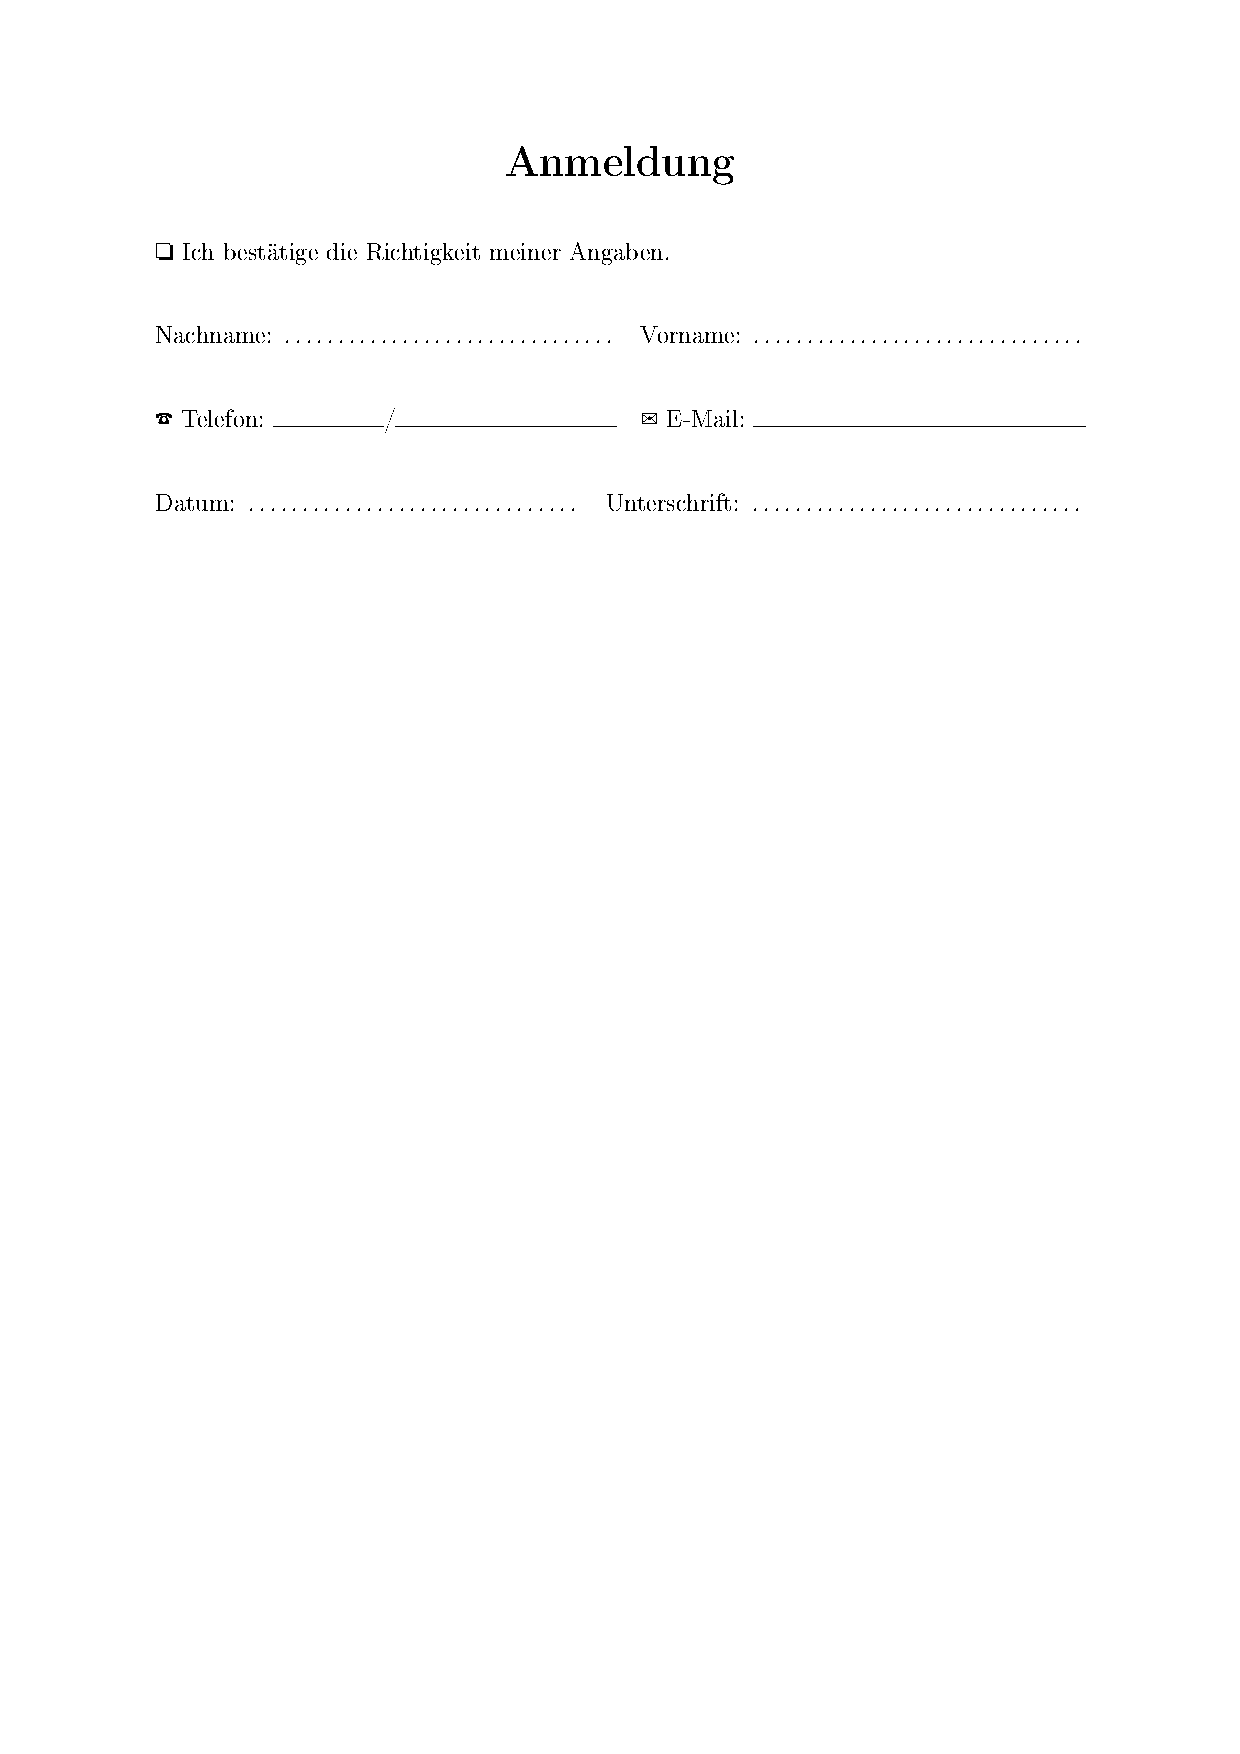
\includegraphics[page=1, clip, trim=2cm 20cm 2cm 2cm, width=.98\textwidth]{Beispiele/Formular/formular_beispiel.pdf}}
	\caption{Resultat von Listing~\ref{formularbeispiel}}
	\label{fig_formularbeispiel}
\end{figure}



\subsection{Grenzen des Textfeldes einhalten}
\index{Textfeld}

Je nach dem Layout des Dokuments und dem zu setzenden Text kann es passieren, das der \LaTeX-Compiler einzelne Wörter über das Textfeld herausragen lässt oder Wortabstände sehr groß erscheinen. In diesem Zusammenhang sind auch Warnungen des \LaTeX-Compilers wie \verb!Overfull \hbox...! und \verb!Underfull \hbox! zu verstehen.

Diese Warnungen können auch im Zusammenhang mit übergroßen oder zu geringen Abständen zwischen Absätzen aufkommen. In diesem Fall enthält die Warnung nicht ein \verb!\hbox!, sondern ein \verb!\vbox!.

Ein Überschreiten des Textfeldes verhindert ein Befehl \verb!\sloppy! in der Präambel des Dokuments. 

\fbox{\texttt{\textbackslash sloppy}}
\index[cmd]{\texttt{\textbackslash sloppy}}  

Dieser Befehl sorgt dafür, das \LaTeX\ bereit ist, Wortabstände wenn nötig weiter zu dehnen als das üblich der Fall ist.

Dem Autor dieser Zeilen ist bewusst, das der Befehl \verb!\sloppy! nicht nur Fans hat, sondern auch an einigen Stellen von seiner
Verwendung abgeraten wird~\cite{LaTeXSuendenregisterLink}. Diese Ablehnung teilt der Autor dieses Werkes aber explizit nicht.

\subsection{Trennungsregeln}
\index{Trennungsregel}

Bei Verwendung der Erweiterungspakete \verb!german! oder \verb|ngerman| hält sich der \LaTeX-Compiler an die deutschen Trennungsregeln.
Gerade bei Fremdwörtern kann es jedoch vorkommen, das Autoren aktiv in die Worttrennung eingreifen müssen.

Eine Möglichkeit ist es, in betreffenden Wörtern mit Hilfe von \verb|\-| manuell Trennungshilfen dort zu definieren, wo Sie ein Wort getrennt
sehen möchten. In der Praxis kann so etwas 
wie folgt aussehen:

\verb!... kommt es zu Durch\-schnitts\-verschiebungen ...!

Diese Trennungshilfen werden nur dann an der konkreten Stelle vom \LaTeX-Compiler berücksichtigt, wenn das Wort am 
Ende einer Zeile steht und getrennt werden muss. Ansonsten sind im fertigen Dokument die im Quelltext eingefügten Trennungshilfen 
zu keiner Zeit erkennbar.

Kommen ein oder mehrere Wörter mit aus Sicht des \LaTeX-Compilers unklarer Worttrennung\index{Worttrennung} mehrfach in einem Dokument vor, ist es sinnvoll
in der Präambel des Dokuments mit dem Befehl \verb!\hyphenation! Trennungsregeln für diese Wörter für das gesamte Dokument zu definieren. 

\fbox{\texttt{\textbackslash hyphenation\{}\textsl{Wort\_1} \textsl{Wort\_2} ... \textsl{Wort\_n}\texttt{\}}}

Die Wörter sind durch Leerzeichen voneinander abgegrenzt. 
Um die Lesbarkeit des Quelltextes an dieser Stelle zu verbessern, kann auch jedes Wort mit einer neuen Zeile beginnen.
In den Wörtern sind die Stellen, an denen Sie dem \LaTeX-Compiler Worttrennungen erlauben, mit Bindestrichen markiert.
Ein Beispiel könnte wie folgt aussehen:

\begin{Verbatim}[frame=single]
\hyphenation{
DHCP-Dis-cover
Durch-schnitts-ver-schiebung 
Pegel-wechsel 
Signal-pegel 
Maxi-mum
Topo-lo-gie
}
\end{Verbatim}


\section{Absätze zentrieren, nach einer Seite ausrichten oder einrücken}

Standardmäßig setzt der \LaTeX-Compiler Texte im \textsl{Blocksatz}\index{Blocksatz}. 
Diese Layoutform ist die am besten lesbare und optisch ansprechendste.
Zudem existiert die Möglichkeit, Text linksbündig, rechtsbündig, zentriert oder beidseitig eingerückt zu setzen. 
Text, der nur nach einer Seite bündig ist, heißt auch \textsl{Flattersatz}\index{Flattersatz}.

Linksbündiger Text ist
ähnlich gut lesbar wie Blocksatz, aber optisch weniger ansprechend. 
Rechtsbündige Texte sind in einigen Kulturkreisen der Standard, im deutschen Sprachraum aber nur selten anzutreffen.
Das zentrieren (also mittiges setzen) von Text ist ein 
häufig angewandtes Stilmittel, um etwas hervorzuheben (z.~B. eine Überschrift).

Zur Realisierung von zentriertem, linksbündigem,
rechtsbündigem oder beidseitig eingerücktem Text existieren jeweils Umgebungen und Befehle.

\subsection{Zentrierter Text}
\index{zentrierter Text}
\index{Text!zentriert}


% \begin{figure}[H]
\begin{minipage}[t]{0.48\textwidth}
\setlength{\parskip}{1em}
\frenchspacing
% \begin{center}
Mit der Umgebung \verb!center!\index[cmd]{\texttt{center}}  
werden beliebige Inhalte (Text, Abbildungen, Tabellen, etc.) zentriert gesetzt.
Alternativ existiert der Befehl \verb!\centering!\index[cmd]{\texttt{\textbackslash centering}}  , der den 
nachfolgenden
Text zentriert setzt. 

Der nebenstehende zentriert gesetzte Text wurde mit der Umgebung \verb!center! erzeugt.
% \end{center}
\end{minipage}
\hfill
\begin{minipage}[t]{0.48\textwidth}
\setlength{\parskip}{1em}
\frenchspacing
\begin{center}
Lorem ipsum dolor sit amet, consectetur adipiscing elit. Curabitur ullamcorper lacus ante, vitae bibendum odio sodales ac. Vestibulum quis pellentesque diam. Aliquam erat volutpat. Nunc gravida vestibulum lacus eu feugiat. Phasellus sit amet tellus nibh. Phasellus lobortis quam vel enim efficitur vestibulum. Duis eleifend eros a erat vehicula porta. Nam.
\end{center}
% \caption{Zentrierter Text}
% \label{Abbildungen_zentrierter_Text}
\end{minipage}
% \end{figure}



\begin{boxedminipage}{\textwidth}
\texttt{\textbackslash begin\{center\}}\dots\texttt{\textbackslash end\{center\}}\\
\texttt{\textbackslash centering} 
\end{boxedminipage}



\subsection{Linksbündiger Text}
\index{linksbündiger Text}
\index{Text!linksbündig}

% \begin{figure}[H]
\begin{minipage}[t]{0.48\textwidth}
\setlength{\parskip}{1em}
\frenchspacing
% \begin{center}
Inhalte linksbündig im Flattersatz setzen die 
Umgebung \verb!flushleft! und alternativ der Befehl \verb!\raggedleft!.
\index[cmd]{\texttt{\textbackslash flushleft}}  
\index[cmd]{\texttt{\textbackslash raggedleft}}  

Der nebenstehende linksbündig gesetzte Text wurde mit der Umgebung \verb!flushleft! erzeugt.
% \end{center}
\end{minipage}
\hfill
\begin{minipage}[t]{0.48\textwidth}
\setlength{\parskip}{1em}
\frenchspacing
\begin{flushleft}
Lorem ipsum dolor sit amet, consectetur adipiscing elit. Curabitur ullamcorper lacus ante, vitae bibendum odio sodales ac. Vestibulum quis pellentesque diam. Aliquam erat volutpat. Nunc gravida vestibulum lacus eu feugiat. Phasellus sit amet tellus nibh. Phasellus lobortis quam vel enim efficitur vestibulum. Duis eleifend eros a erat vehicula porta. Nam.
\end{flushleft}
\end{minipage}
% \end{figure}




\begin{boxedminipage}{\textwidth}
\texttt{\textbackslash begin\{flushleft\}}\dots\texttt{\textbackslash end\{flushleft\}}\\
\texttt{\textbackslash raggedleft} 
\end{boxedminipage}


\subsection{Rechtsbündiger Text}
\index{rechtsbündiger Text}
\index{Text!rechtsbündig}


% \begin{figure}[H]
\begin{minipage}[t]{0.48\textwidth}
\setlength{\parskip}{1em}
\frenchspacing
% \begin{center}
Inhalte rechtsbündig im Flattersatz setzen die 
Umgebung \verb!flushright! und alternativ der Befehl \verb!\raggedright!.
\index[cmd]{\texttt{\textbackslash flushright}}  
\index[cmd]{\texttt{\textbackslash raggedright}}  

Der nebenstehende rechtsbündig gesetzte Text wurde mit der Umgebung \verb!flushright! erzeugt.
% \end{center}
\end{minipage}
\hfill
\begin{minipage}[t]{0.48\textwidth}
\setlength{\parskip}{1em}
\frenchspacing
\begin{flushright}
Lorem ipsum dolor sit amet, consectetur adipiscing elit. Curabitur ullamcorper lacus ante, vitae bibendum odio sodales ac. Vestibulum quis pellentesque diam. Aliquam erat volutpat. Nunc gravida vestibulum lacus eu feugiat. Phasellus sit amet tellus nibh. Phasellus lobortis quam vel enim efficitur vestibulum. Duis eleifend eros a erat vehicula porta. Nam.
\end{flushright}
\end{minipage}
% \end{figure}




\begin{boxedminipage}{\textwidth}
\texttt{\textbackslash begin\{flushright\}}\dots\texttt{\textbackslash end\{flushright\}}\\
\texttt{\textbackslash raggedright} 
\end{boxedminipage}



\subsection{Beidseitig eingerückter Text}
\index{eingerückter Text}
\index{Text!eingerückt}

Besonders bei Zitaten ist es optisch ansprechend, wenn der Text beidseitig gleich weit eingerürückt ist, um ihn dadurch hervorzuheben. Zu diesem Zweck 
existierenden die beiden Umgebungen \verb!quote! und alternativ \verb!quotation!.
\index[cmd]{\texttt{quote}}  
\index[cmd]{\texttt{quotation}}  

Der folgende beidseitig gleich weit eingerückt gesetzte Text wurde mit der Umgebung \verb!quote! erzeugt.

\begin{quote}
	Lorem ipsum dolor sit amet, consectetur adipiscing elit. 
	
	Curabitur ullamcorper lacus ante, vitae bibendum odio sodales ac. 
	
	Vestibulum quis pellentesque diam. Aliquam erat volutpat. 
\end{quote}

Die Umgebung \verb!quote! fügt automatisch zwischen Absätzen einen vertikalen Abstand ein und rückt die erste Zeile eines jeden Absatzes nicht ein. 

\fbox{
	\texttt{\textbackslash begin\{quote\}}\dots\texttt{\textbackslash end\{quote\}}
}

Das Verhalten von \verb!quote! entspricht damit dem Standard im deutschen Sprachraum.

Der folgende beidseitig gleich weit eingerückt gesetzte Text wurde mit der Umgebung \verb!quotation! erzeugt.

\begin{quotation}
	Lorem ipsum dolor sit amet, consectetur adipiscing elit. 
	
	Curabitur ullamcorper lacus ante, vitae bibendum odio sodales ac. 
	
	Vestibulum quis pellentesque diam. Aliquam erat volutpat. 
\end{quotation}

Die Umgebung \verb!quotation! rückt die erste Zeile eines jeden Absatzes ein und verzichtet dafür auf den vertikalen Abstand zwischen Absätzen. 

\fbox{\texttt{\textbackslash begin\{quotation\}}\dots\texttt{\textbackslash end\{quotation\}}}

Das Verhalten von \verb!quotation! entspricht damit dem Standard im anglo-amerikanischen Sprachraum.




\section{Zeilenumbrüche}
\index{Zeilenumbruch} 

Ein Zeilenumbruch 
kann an beliebiger Stelle im Text mit dem
Befehl \verb!\\!\index[cmd]{\texttt{\textbackslash\textbackslash}} realisiert werden. Zudem ist es möglich, mit dem 
optionalen Parameter \textsl{Abstand} den vertikalen Zwischenraum zur nächsten Zeile anzugeben. Wenn durch
den Parameter \textsl{Abstand} ein Seitenumbruch zustande kommt, dann wird 
der Inhalt von \textsl{Abstand} vom \LaTeX-Compiler ignoriert und die nächste Seite 
beginnt mit der nächsten Textzeile. 

\begin{boxedminipage}{\textwidth}
	\texttt{\textbackslash \textbackslash[}\textsl{Abstand}\texttt{]}
\end{boxedminipage}


Eine Variante des Befehls \verb!\\! ist der Befehl 
\verb!\\*!. Dieser verhindert, dass nach
dem Zeilenumbruch ein Seitenwechsel 
vor der nächsten Textzeile erscheint.


\begin{boxedminipage}{\textwidth}
	\texttt{\textbackslash \textbackslash*[}\textsl{Abstand}\texttt{]} 
\end{boxedminipage}


Enthält ein Dokument beispielsweise den Befehl 
\verb!\\[1cm]!, dann wird der \LaTeX-Compiler einen Zeilenumbruch 
mit einen vertikalen Zeilenabstand von 1\,cm 
einfügen. Kommt durch diesen  Befehl ein 
Seitenumbruch zustande, dann 
wird der \LaTeX-Compiler auf der neuen Seite die 
dem Befehl vorangegangene Zeile 
setzen, dann den 1\,cm großen Abstand einfügen und danach die nächste Zeile. 


Eine weitere Variante ist der 
Befehl \verb!\newline!\index[cmd]{\texttt{\textbackslash newline}}, 
dessen Verhalten mit dem des Befehls \verb!\\! identisch ist. 
Mit \verb!\newline! ist es allerdings nicht möglich, den 
Zwischenraum zur nächsten Zeile zu definieren.


\fbox{\texttt{\textbackslash newline}}




\section{Seitenumbrüche}
\index{Seitenumbruch}

Genau wie beim Zeilenumbruch wird auch 
der Seitenumbruch vom \LaTeX-Compiler selbst
vorgenommen. Er versucht eventuell vorhandene
Gleitobjekte wie Bilder und Tabellen an der geeignetsten Position 
zu setzen, damit es nicht zu den so genannten
\textsl{Hurenkindern} oder \textsl{Schusterjungen} kommt (siehe Abschnitt~\ref{Absatzabstand}),

In seltenen Fällen kann es aber sinnvoll sein,
einen Seitenumbruch an einer bestimmten Stelle anzuweisen.


Der Befehl \verb!\newpage!\index[cmd]{\texttt{\textbackslash newpage}}  
beendet bei einem einspaltigen Seitenlayout 
die aktuelle Seite und bei einem zweispaltigen 
Layout die aktuelle Spalte. 


\fbox{\texttt{\textbackslash newpage}}

Das manuelle Umbrechen der aktuelle Seite bei eine zweispaltigen Seitenlayout (Klassenoption \verb!twocolumn! oder Befehl \verb!\twocolumn!) geschieht mit dem Befehl \verb!\clearpage!.\index[cmd]{\texttt{\textbackslash clearpage}}  

\fbox{\texttt{\textbackslash clearpage}}

Bei einem doppelseitigem Layout (Klassenoption \verb!twoside!) geschieht das manuelle Umbrechen der aktuelle Seite mit dem Befehl 
\verb!\cleardoublepage!.\index[cmd]{\texttt{\textbackslash cleardoublepage}}  
Dieser garantiert, das die nächste Seite, auf der sich Inhalte befinden, eine ungerade (linke) Seite ist.

\fbox{\texttt{\textbackslash cleardoublepage}}

In bestimmten Situationen kann es hilfreich sein, einen Seitenumbruch an einer bestimmten Stelle zu untersagen. Zu diesem Zweck existiert der Befehl \verb!nopagebreak!.

\fbox{\texttt{\textbackslash nopagebreak}}
\index[cmd]{\texttt{\textbackslash nopagebreak}}  

	
\chapter{Texthervorhebungen}
\label{KapitelTexthervorhebungen}
\index{Texthervorhebungen}

Texthervorhebungen ermöglichen es, bestimmte 
Textstellen von anderen abzugrenzen oder hervorzuheben. Konkret beschreibt dieses
Kapitel unter anderem, Möglichkeiten um Schriftarten und Schriftgröße zu verändern, 
Texte zu unterstreichen und die Lesbarkeit von Texte mit Aufzählungen zu verbessern.

\section{Texte hervorheben}

Das \emph{Hervorheben} kurzer Textstellen (einzelner Wörter oder Sätze) geschieht 
mit dem Befehl \verb!\emph!\index[cmd]{\texttt{\textbackslash emph}}  
oder alternativ mit der Umgebung \verb!em!\index[cmd]{\texttt{em}}. 
Beide heben den betreffenden Text durch einen Wechseln des Schriftschnitts\index{Schriftschnitt} hervor.

\begin{boxedminipage}{\textwidth}
\texttt{\textbackslash emph\{\textsl{Text}\}}\\
\texttt{\textbackslash begin\{em\}} \enskip \textsl{Text} \enskip \texttt{\textbackslash end\{em\}}
\end{boxedminipage}

Bei einer senkrechten Grundschrift stellt \verb!\emph! den 
\emph{hervorzuhebenden Text} mit einer \textsl{kursiven Schrift} dar. 
Bei einer kursiven Grundschriftart ist es genau 
umgekehrt. Hier wird der hervorgehobene Text mit einer senkrechten 
Schriftart dargestellt.

Der Wechsel des Schriftschnitts sieht weniger aufdringlich aus als das
klassische \underline{Unterstreichen} mit dem Befehl \verb!\underline!.\index[cmd]{\texttt{\textbackslash underline}}  

\fbox{\texttt{\textbackslash underline\{\textsl{Text}\}}}

Ein Nachteil des Befehls \verb!\underline! ist, das er keinen Zeilenumbruch zulässt, weil er den kompletten Inhalt des Arguments \textsl{Text} in einer horizontale Box unterbringt. Darum eignet sich \verb!\underline! in erster Linie zur Hervorhebung einzelner Zeichen oder Wörter.

Weitere Befehle, um Text hervorzuheben, enthält das Erweiterungspaket \verb!ulem.sty!. 
Wird dieses in der Präambel eines Dokuments mit dem Befehl \verb!\usepackage{ulem}! eingebunden, steht eine Reihe 
weiterer Befehle zur Verfügung.

Dieses sind die Befehle \verb!\uline!\index[cmd]{\texttt{\textbackslash uline}}  
zum \uline{Unterstreichen}, \verb!\uuline!\index[cmd]{\texttt{\textbackslash uuline}}  
zum \uuline{Doppeltunterstreichen}, \verb!\uwave!\index[cmd]{\texttt{\textbackslash uwave}}  
zum \uwave{Unterstreichen mit Wellen}, \verb!\sout!\index[cmd]{\texttt{\textbackslash sout}}  
zum \sout{Durchstreichen}, \verb!\xout!\index[cmd]{\texttt{\textbackslash xout}}  
zum \xout{Ausstreichen}, \verb!\dashuline!\index[cmd]{\texttt{\textbackslash dashuline}}  
zum  \dashuline{Unterstreichen mit kurzen Strichen} und \verb!\dotuline!\index[cmd]{\texttt{\textbackslash dotuline}}  
zum  \dotuline{Unterstreichen mit einer Linie aus Punkten}

\begin{boxedminipage}{\textwidth}
\texttt{\textbackslash uline\{}\textsl{Text}\texttt{\}} \\
\texttt{\textbackslash uuline\{}\textsl{Text}\texttt{\}} \\
\texttt{\textbackslash uwave\{}\textsl{Text}\texttt{\}} \\
\texttt{\textbackslash sout\{}\textsl{Text}\texttt{\}} \\
\texttt{\textbackslash xout\{}\textsl{Text}\texttt{\}} \\
\texttt{\textbackslash dashuline\{}\textsl{Text}\texttt{\}} \\
\texttt{\textbackslash dotuline\{}\textsl{Text}\texttt{\}} 
\end{boxedminipage}

Da diese Befehle aus dem Erweiterungspaket \verb!ulem.sty! jedes Wort in einer eigenen Box verpacken, sind innerhalb des  Arguments \textsl{Text} Zeilenumbrüche möglich.

Eine Eigenheit des Erweiterungspakets \verb!ulem.sty! ist, dass es das Verhalten des Befehls \verb!\emph! dahingehend ändert, das der \LaTeX-Compiler mit \verb!\emph! betonte Wörter nicht mehr kursiv, sondern unterstrichen setzt. Mit dem Befehl \verb!\normalem! nach dem \verb!\begin{document}! kann das \emph{normale} Verhalten des Befehls \verb!\emph! wiederhergestellt werden.

\section{Schriftgrößen}

Zur Definition der Schriftgröße existiert eine Reihe von Befehlen (siehe Tabelle~\ref{Tabelle_Schriftgroesse})
Diese Befehle gelten ab der Position, wo sie im Quelltext aufgerufen werden. Die so ausgewählte Schriftgröße bleibt so lange aktuell, bis das 
Ende der Gruppe oder das Ende des Dokuments erreicht ist oder bis durch einen Befehl
eine neue Schriftgröße festlegt wird.

\begin{table}[htb]
\centering
\caption{Befehle zur Definition der Schriftgröße}
\index[cmd]{\texttt{\textbackslash tiny}}  
\index[cmd]{\texttt{\textbackslash scriptsize}}  
\index[cmd]{\texttt{\textbackslash footnotesize}}  
\index[cmd]{\texttt{\textbackslash small}}  
\index[cmd]{\texttt{\textbackslash normalsize}}  
\index[cmd]{\texttt{\textbackslash large}}  
\index[cmd]{\texttt{\textbackslash Large}}  
\index[cmd]{\texttt{\textbackslash LARGE}}  
\index[cmd]{\texttt{\textbackslash huge}}  
\index[cmd]{\texttt{\textbackslash Huge}}  
\label{Tabelle_Schriftgroesse}       % Give a unique label
\begin{tabular}{ll}
\hline
Befehl & Beispiel \\
\hline
\texttt{\textbackslash tiny} & {\tiny ABCDEFGHI0123456789} \\
\texttt{\textbackslash scriptsize} & {\scriptsize ABCDEFGHI0123456789} \\
\texttt{\textbackslash footnotesize} & {\footnotesize ABCDEFGHI0123456789} \\
\texttt{\textbackslash small} & {\small ABCDEFGHI0123456789} \\
\texttt{\textbackslash normalsize} & {\normalsize ABCDEFGHI0123456789} \\
\texttt{\textbackslash large} & {\large ABCDEFGHI0123456789} \\
\texttt{\textbackslash Large} & {\Large ABCDEFGHI0123456789} \\
\texttt{\textbackslash LARGE} & {\LARGE ABCDEFGHI0123456789} \\
\texttt{\textbackslash huge} & {\huge ABCDEFGHI0123456789} \\
\texttt{\textbackslash Huge} & {\Huge ABCDEFGHI0123456789} \\
\hline
\end{tabular}
\end{table}

\section{Schriftfamilien und Schriftschnitte}
\label{AbschnittSchriftfamilienSchriftschnitte}

Tabelle~\ref{Tabelle_SchriftfamilieSchriftschnittMitArgument} zeigt Befehle zur Definition der Schrift, die den betreffenden Text als Argument übergeben bekommen.

\begin{table}[h!tb]
\centering
\caption{Befehle zur Definition der Schrift mit Text als Argument}
\index[cmd]{\texttt{\textbackslash textrm}}  
\index[cmd]{\texttt{\textbackslash texttt}}  
\index[cmd]{\texttt{\textbackslash textsf}}  
\index[cmd]{\texttt{\textbackslash textsc}}  
\index[cmd]{\texttt{\textbackslash textsl}}  
\index[cmd]{\texttt{\textbackslash textit}}  
\index[cmd]{\texttt{\textbackslash textup}}  
\index[cmd]{\texttt{\textbackslash textmd}}  
\index[cmd]{\texttt{\textbackslash textbf}}  
\label{Tabelle_SchriftfamilieSchriftschnittMitArgument}       % Give a unique label
\begin{tabular}{ll}
\hline
Befehl & Beschreibung \\
\hline
\texttt{\textbackslash textrm\{\textsl{Text}\}} & \textrm{schaltet auf die Schriftart Roman} \\
\texttt{\textbackslash texttt\{\textsl{Text}\}} & \texttt{schaltet auf eine Schreibmaschinenschrift (Typewriter)} \\
\texttt{\textbackslash textsf\{\textsl{Text}\}} & \textsf{schaltet auf die Sans-Serif-Schriftfamilie} \\
\texttt{\textbackslash textsc\{\textsl{Text}\}} & \textsc{schaltet auf Kapitälchen-Schrift (Small Caps)} \\
\texttt{\textbackslash textsl\{\textsl{Text}\}} & \textsl{schaltet auf geneigte Roman-Schrift (Slanted)} \\
\texttt{\textbackslash textit\{\textsl{Text}\}} & \textit{schaltet auf die Schrift Italic} \\
\texttt{\textbackslash textup\{\textsl{Text}\}} & \textup{schaltet auf senkrechten Schriftschnitt} \\
\texttt{\textbackslash textmd\{\textsl{Text}\}} & \textmd{schaltet auf normale Breite und Strichstärke (normale Schrift)} \\
\texttt{\textbackslash textbf\{\textsl{Text}\}} & \textbf{schaltet auf fette Schrift} \\
\hline
\end{tabular}
\end{table}

Während die Befehle aus Tabelle~\ref{Tabelle_SchriftfamilieSchriftschnittMitArgument} mit dem Text als Argument sich eher für kürzere Texte eignen, sind die Deklarationsbefehle aus Tabelle~\ref{Tabelle_SchriftfamilieSchriftschnittOhneArgument} zum Umschalten der Schrift für längere Texte besser geeignet.

\begin{table}[h!tb]
\centering
\caption{Befehle zur Definition der Schrift und die entsprechenden Umgebungen}
\label{Tabelle_SchriftfamilieSchriftschnittOhneArgument}       % Give a unique label
\begin{tabular}{lcl}
\hline
Befehl & Umgebung & Beispiel \\
\hline
\texttt{\textbackslash rmfamily} & \texttt{\textbackslash begin\{rmfamily\}} \enskip \textsl{Text} \enskip \texttt{\textbackslash end\{rmfamily\}} & {\rmfamily Roman} \\
\texttt{\textbackslash ttfamily} & \texttt{\textbackslash begin\{ttfamily\}} \enskip \textsl{Text} \enskip \texttt{\textbackslash end\{ttfamily\}} & {\ttfamily Typewriter} \\
\texttt{\textbackslash sffamily} & \texttt{\textbackslash begin\{sffamily\}} \enskip \textsl{Text} \enskip \texttt{\textbackslash end\{sffamily\}} & {\sffamily Sans Serif} \\
\texttt{\textbackslash scshape} & \texttt{\textbackslash begin\{scshape\}} \enskip \textsl{Text} \enskip \texttt{\textbackslash end\{scshape\}} & {\scshape Small Caps} \\
\texttt{\textbackslash slshape} & \texttt{\textbackslash begin\{slshape\}} \enskip \textsl{Text} \enskip \texttt{\textbackslash end\{slshape\}} & {\slshape Slanted} \\
\texttt{\textbackslash itshape} & \texttt{\textbackslash begin\{itshape\}} \enskip \textsl{Text} \enskip \texttt{\textbackslash end\{itshape\}} & {\itshape Italic} \\
\texttt{\textbackslash upshape} & \texttt{\textbackslash begin\{upshape\}} \enskip \textsl{Text} \enskip \texttt{\textbackslash end\{upshape\}} & {\upshape Senkrechte Schrift} \\
\texttt{\textbackslash mdseries} & \texttt{\textbackslash begin\{mdseries\}} \enskip \textsl{Text} \enskip \texttt{\textbackslash end\{mdseries\}} & {\mdseries Normale Schrift} \\
\texttt{\textbackslash bfseries} & \texttt{\textbackslash begin\{bfseries\}} \enskip \textsl{Text} \enskip \texttt{\textbackslash end\{bfseries\}} & {\bfseries Fette Schrift} \\
\hline
\end{tabular}
\index[cmd]{\texttt{\textbackslash rmfamily}}
\index[cmd]{\texttt{\textbackslash ttfamily}}
\index[cmd]{\texttt{\textbackslash sffamily}}
\index[cmd]{\texttt{\textbackslash scshape}}
\index[cmd]{\texttt{\textbackslash slshape}}
\index[cmd]{\texttt{\textbackslash slshape}}
\index[cmd]{\texttt{\textbackslash itshape}}
\index[cmd]{\texttt{\textbackslash upshape}}
\index[cmd]{\texttt{\textbackslash mdseries}}
\index[cmd]{\texttt{\textbackslash bfseries}}
\end{table}

Die Befehle in Tabelle~\ref{Tabelle_SchriftfamilieSchriftschnittOhneArgument} schalten die Schrift an der Stelle 
ihres Auftretens im \LaTeX-Quelltext um. 
Die Wirkung dieser Befehle ist durch die aktuelle Gruppe
begrenzt. Ein Aufruf eines dieser Befehle in der Präambel eines Dokuments
beeinflusst das gesamte Dokument. 

Nach eine Änderung der Schrift kann mit dem Befehl \verb!\textnormal!\index[cmd]{\texttt{\textbackslash textnormal}} 
jederzeit auf die alte Schrift zurückgegriffen werden, die zu Beginn des Dokuments gültig war. 

\fbox{\texttt{\textbackslash textnormal\{\textsl{Text}\}}}

Die Umgebungen in Tabelle~\ref{Tabelle_SchriftfamilieSchriftschnittOhneArgument} eignen sich besonders dann, wenn für einzelne Abschnitte eines Dokuments die Schrift angepasst werden soll. 

\section{Aufzählungen}
\label{Abschnitt_Aufzaehlungen}
\index{Aufzählung}

Das Setzen von Aufzählungen geschieht mit den Umgebungen 
\verb!itemize!\index[cmd]{\texttt{itemize}}, 
\verb!enumerate!\index[cmd]{\texttt{enumerate}} und 
\verb!description!\index[cmd]{\texttt{description}}. Alle
diese Umgebungen rücken den aufgezählten Text ein wenig ein und versehen ihn am Anfang mit einer Markierung (einem Zeichen).

\begin{boxedminipage}{\textwidth}
	\texttt{\textbackslash begin\{itemize\}} \enskip \dots\ \enskip \texttt{\textbackslash end\{itemize\}} \\
	\texttt{\textbackslash begin\{enumerate\}} \enskip \dots\ \enskip \texttt{\textbackslash end\{enumerate\}} \\
	\texttt{\textbackslash begin\{description\}} \enskip \dots\ \enskip \texttt{\textbackslash end\{description\}}
\end{boxedminipage}

Während \verb!itemize! jedes neue Element der Aufzählung mit einem schwarzen,
ausgefüllten Punkt \textbullet\ kennzeichnet, nummeriert \verb!enumerate! die 
Elemente durch. \verb!description! hingegen hebt einen vom Autor festzulegenden 
Text am Anfang des Elements hervor.

Bei allen diesen drei Umgebungen wird jeder neue Element der Aufzählung durch
den Befehl \verb!\item!\index[cmd]{\texttt{\textbackslash item}} gekennzeichnet. Der Text jedes Elements -- man könnte auch Aufzählungspunktes\index{Aufzählungspunkt} sagen -- darf beliebig lang sein, und kann auch aus
mehreren Absätzen bestehen. 

Alle in diesem Abschnitt beschrieben Umgebungen können verschachtelt werden. Mehr als vier Ebenen sind aber nicht zulässig. 

Bei der Umgebung \verb!itemize! ist für jede Ebene ein Markierungszeichen voreingestellt. Die folgende Übersicht zeigt, welche das im Einzelnen sind.

% \begin{figure}[H]
\begin{minipage}[h]{0.44\textwidth}
\setlength{\parskip}{1em}
\frenchspacing
\begin{Verbatim}[frame=single]
\begin{itemize}
\item In der ersten Ebene...
\begin{itemize}
\item In der zweiten Ebene
ist es ein...
\begin{itemize}
\item In der dritten Ebene
ist das Markierungszeichen...
\begin{itemize}
\item In der vierten Ebene 
ist es ein...
\end{itemize}
\end{itemize}
\end{itemize}
\end{itemize}
\end{Verbatim}
\end{minipage}
\hfill
\begin{minipage}[h]{0.54\textwidth}
\setlength{\parskip}{1em}
\frenchspacing
\begin{itemize}
\item In der ersten Ebene von \texttt{itemize} ist das Markierungszeichen ein sogenannter
\texttt{\textbackslash textbullet}.
\begin{itemize}
\item In der zweiten Ebene ist es ein fett geschriebener Trennstrich
\texttt{\{\textbackslash normalfont\textbackslash bfseries \textbackslash textendash\}}.
\begin{itemize}
\item In der dritten Ebene ist das Markierungszeichen ein \texttt{\textbackslash textasteriskcentered}.
\begin{itemize}
\item In der vierten Ebene ist es ein \texttt{\textbackslash textperiodcentered}. 
\end{itemize}
\end{itemize}
\end{itemize}
\end{itemize}
\end{minipage}
% \end{figure}

Aufzählungen realisiert die Umgebung \verb!enumerate!. Auch bei \verb!enumerate! ist für jede Ebene eine andere Art von Markierungszeichen voreingestellt und die Nummerierung der Aufzählungspunkte startet in jeder Ebene neu beim Wert \verb!1!.

% \begin{figure}[H]
\begin{minipage}[h]{0.44\textwidth}
\setlength{\parskip}{1em}
\frenchspacing
\begin{Verbatim}[frame=single]
\begin{enumerate}
\item In der ersten Ebene...
\item arabischen Ziffern...
\begin{enumerate}
\item Die zweite Ebene...
\item Buchstaben und...
\begin{enumerate}
\item Die dritte Ebene...
\item römische Ziffern.
\begin{enumerate}
\item Die vierte Ebene nutzt 
\item großen Buchstaben.
\end{enumerate}
\item Beim Verschachteln...
\end{enumerate}
\end{enumerate}
\end{enumerate}
\end{Verbatim}
\end{minipage}
\hfill
\begin{minipage}[h]{0.54\textwidth}
\setlength{\parskip}{1em}
\frenchspacing
\begin{enumerate}
\item In der ersten Ebene wird mit
\item arabischen Ziffern durchnummeriert.
\begin{enumerate}
\item Die zweite Ebene verwendet kleine
\item Buchstaben und schließende Klammern.
\begin{enumerate}
\item Die dritte Ebene verwendet
\item römische Ziffern.
\begin{enumerate}
\item Die vierte Ebene nutzt 
\item großen Buchstaben.
\end{enumerate}
\item Beim Verschachteln gehen die Zählerstände nicht verloren.
\end{enumerate}
\end{enumerate}
\end{enumerate}
\end{minipage}
% \end{figure}

Die Umgebung \verb!description! ist ideal um Begriffe (Schlagwort) zu beschreiben oder Teilnehmerlisten zu realisieren. Diese Umgebung unterscheidet sich in einigen Punkten von \verb!itemize! und \verb!enumerate!.
Bei \verb!description! wird zwischen dem Befehl \verb!\item! und der Beschreibung das Schlagwort in eckigen Klammern angegeben. Die Ausgabe des Schlagworts erfolgt im Fettdruck. 

% \begin{figure}[H]
\begin{minipage}[h]{0.44\textwidth}
\setlength{\parskip}{1em}
\frenchspacing
\begin{Verbatim}[frame=single]
\begin{description}
\item[Bit] Kleinstmögliche...
\item[Byte] Gruppe von 8...
\item[Nibble] Gruppe von 4...
\item[Oktett] siehe Byte...
\item[Unicode] Mehrbyte....
\end{description}
\end{Verbatim}
\end{minipage}
\hfill
\begin{minipage}[h]{0.54\textwidth}
\setlength{\parskip}{1em}
\frenchspacing
\begin{description}
\item[Bit] Kleinstmögliche Informationseinheit. Zwei mögliche Zustände
\item[Byte] Gruppe von 8\,Bits
\item[Nibble] Gruppe von 4\,Bits bzw. ein Halbbyte
\item[Oktett] siehe Byte
\item[Unicode] Mehrbyte-Zeichenkodierung
\end{description}
\end{minipage}
% \end{figure}

\section{Fußnoten}
\index{Fußnote}

Das Erzeugen von Fußnoten geschieht mit dem Befehl \verb!\footnote!\index[cmd]{\texttt{\textbackslash footnote}}. 

\fbox{\texttt{\textbackslash footnote\{}\textsl{Text in der Fußnote}\texttt{\}}}

Der Befehl \verb!\footnote! folgt im Quelltext immer direkt -- also ohne
Leerzeichen -- nach dem Wort, an das die Markierung der Fußnote angehängt sein soll. Der
Text der Fußnote wird vom \LaTeX-Compiler in einer kleineren Schrift von der Größe  
{\footnotesize footnotesize} geschrieben. 
Standardmäßig rückt der \LaTeX-Compiler die erste
Zeile einer Fußnote einen halben Zentimeter ein. 

Zwischen den
Fußnoten einer Seite und dem gewöhnlichen 
Text des Dokuments fügt der \LaTeX-Compiler automatisch eine
horizontale Linie ein, um die Fußnoten deutlich vom Text abzuheben. 

Der Befehl \verb!\footnote! darf nicht innerhalb mathematischer 
Umgebungen oder Tabellen aufgerufen werden. Es gibt aber verschiedene Tricks, um sich in einem solchen Fall zu behelfen. Eine Möglichkeit, um Fußnoten in von Tabellen zu realisieren, sind die Befehle \verb!\footnotemark!\index[cmd]{\texttt{\textbackslash footnotemark}} 
zum Erzeugen einer einzelne Fußnotenmarkierung und \verb!\footnotetext!\index[cmd]{\texttt{\textbackslash footnotetext}} 
zum Erzeugt eines einzelnen Fußnotentextes für eine bestimmte Fußnotenmarkierung.

\section{Marginalien}
\index{Marginalie}
\index{Randbemerkung}
\index{Randnotiz} 

Randbemerkungen, die auch \emph{Marginalien} heißen, 
sind ein mögliches Stilmittel für 
Ergänzungen und Erläuterungen.   

\fbox{\texttt{\textbackslash marginpar[}\textsl{Text einer linken Randnotiz}\texttt{]\{}\textsl{Text einer rechten Randnotiz}\texttt{\}}}

Bei\marginpar{Die erste Zeile des Textes der Marginalie wird von \LaTeX\ in der gleichen Zeile gesetzt, in der sich der Befehl \texttt{\textbackslash marginpar} befindet.} einem Text mit zweispaltigem Layout wird die Randbemerkung an den am 
nächsten liegenden Rand gesetzt.
Mit Hilfe der drei Befehle \verb!\marginparwidth!\index[cmd]{\texttt{\textbackslash marginparwidth}}, 
\verb!\marginparsep! \index[cmd]{\texttt{\textbackslash marginparsep}}und 
\verb!\marginparpush!\index[cmd]{\texttt{\textbackslash marginparpush}} ist es möglich, das Aussehen der Marginalien zu beeinflussen.
Jeder der drei Befehle erfordert die Angabe einer Breite bzw. eines Abstands inklusive einer Maßeinheit (siehe Abschnitt~\ref{sec:Massangaben}) in geschweiften Klammern.

Der Befehl \verb!\marginparwidth! definiert die Breite des Randnotizen-Bereichs fest.

\fbox{\texttt{\textbackslash setlength\{\textbackslash marginparwidth\}\{\textsl{Breite}\texttt{\}}}}

Der Befehl \verb!\marginparsep! definiert den Abstand zwischen Textfeld und Randnotizen.

\fbox{\texttt{\textbackslash setlength\{\textbackslash marginparsep\}\{\textsl{Abstand}\texttt{\}}}}

Der Befehl \verb!\marginparpush! definiert den Abstand zwischen zwei Randnotizen.

\fbox{\texttt{\textbackslash setlength\{\textbackslash marginparpush\}\{\textsl{Abstand}\texttt{\}}}}

\section{Unformatierter Text}
\index{Text!unformatierter}
\index{Unformatierter Text}

Die Möglichkeit, unformatierten Text in einem Dokument einzufügen, ist 
besonders für Dokumentationen und wissenschaftliche 
Publikationen im Bereich der Informatik hilfreich, denn
Programmcode wird auf diese Art und Weise 
vom übrigen Text abgehoben.
Auch in diesem Dokument sind Befehle und Umgebungen auf diese Art und Weise dargestellt.

Das Setzen von unformatiertem Text kann u.a. mit der Umgebung \verb!verbatim!\index[cmd]{\texttt{verbatim}} 
geschehen. 

\fbox{\texttt{\textbackslash begin\{verbatim\}}\textsl{Text}\texttt{\textbackslash end\{verbatim\}}}

Text, der sich innerhalb dieser Umgebung befindet, wird vom \LaTeX-Compiler in \verb!TypeWriter!, also \verb!Schreibmaschinenschrift! gesetzt und nicht verändert oder interpretiert.
Dieser Text kann somit alle Sonderzeichen von \LaTeX\ 
und beliebige Kombinationen von Leerzeichen und Zeilenumbrüchen enthalten. 

Zu Beginn und Ende der Umgebung \verb!verbatim! fügt der \LaTeX-Compiler einen
vertikalen Leerraum ein und es wird zu
Anfang und Ende der Umgebung eine neue Zeile begonnen.

Eine weitere Möglichkeit, unformatierten,
maximal eine Zeile langen Text auszugeben ist der Befehl \verb!\verb!\index[cmd]{\texttt{\textbackslash verb}}.
Direkt im Anschluss an den Befehl muss ein zur Abgrenzung verwendetes Zeichen folgen.
Dieses Begrenzungszeichen muss den unformatiert auszugebenden Text auch abschließen. 
In der folgenden Darstellung der Syntax von \verb!\verb! dient das Zeichen \verb|+| als Begrenzungszeichen.

\fbox{\texttt{\textbackslash verb}+\textsl{Text}+}

Anstelle des Zeichens \verb|+| könnte auch das Zeichen \verb?!?, \verb#?#, \verb<#< oder \verb!|! oder sonst (fast) ein beliebiges Zeichen als Begrenzungszeichen
verwendet werden. Das Begrenzungszeichen darf sich
aber nicht im darzustellenden Text befinden und die 
Begrenzungszeichen eines \verb!\verb!-Befehls müssen sich 
in einer Zeile im Quelltext befinden. 

Weder die Umgebung \verb!verbatim!, noch Varianten davon wie der Befehl \verb!\verb! dürfen in Argumenten von Befehlen oder innerhalb von Tabellen verwendet werden.

\section{Internetadressen}
\index{Internetadressen}
\index{URL}

Zum Satz von Internetadressen (URL) existiert das Erweiterungspaket \verb!url!. Wird dieses mit dem Befehl \verb!\usepackage{url}! in der Präambel der Quelldatei eingebunden, steht der gleichnamige Befehl \verb!\url!\index[cmd]{\texttt{\textbackslash url}} zur Verfügung. Diesem wird die zu setzende
Internetadresse in geschweiften Klammern als Parameter übergeben. 

\fbox{\texttt{\textbackslash url\{}\textsl{Internatadresse}\texttt{\}}}

Die Adresse setzt der \LaTeX-Compiler dann in einer Schrift mit fester Zeichenbreite und bricht die Adressen bei Bedarf optisch ansehnlich um.
Zudem sind mit dem Befehl \verb!\url! realisierte Internetadressen in der resultierenden PDF-Datei als Link nutzbar.

\section{Boxen um Text und Bilder zeichnen}
\label{Abschnitt_Boxen}
\index{Boxen}

Boxen sind eine einfache Möglichkeit, um Textabschnitte oder Bilder hervorzuheben. 
Ein Beispiel für einen Befehl, der es ermöglicht, einen Kasten um einen zu umrahmenden Text zu setzen, ist \verb!\fbox!.

\fbox{\texttt{\textbackslash fbox\{\textsl{Text}\}}}

Ein Nachteil dieses Befehls ist, das damit weder die Größe der Box, noch die Ausrichtung des Textes beeinflusst werden können.

Ausgefallenere Boxentypen bietet das Erweiterungspaket \verb!fancybox!\index[cmd]{\texttt{fancybox}}. Wird es mit dem Befehl \verb!\usepackage{fancybox}! in der Präambel der \verb!.tex!-Quelldatei eingebunden, stehen die Befehle \verb!\doublebox!, \verb!\ovalbox!, \verb!\Ovalbox! und \verb!\shadowbox! zur Verfügung.

\begin{center}
\doublebox{\texttt{\textbackslash doublebox}}\index[cmd]{\texttt{\textbackslash doublebox}}  
\hspace{5mm}
\ovalbox{\texttt{\textbackslash ovalbox}}\index[cmd]{\texttt{\textbackslash ovalbox}}   
\hspace{5mm}
\Ovalbox{\texttt{\textbackslash Ovalbox}} 
\hspace{5mm}
\shadowbox{\texttt{\textbackslash shadowbox}}\index[cmd]{\texttt{\textbackslash shadowbox}}   
\end{center}

\begin{boxedminipage}{\textwidth}
\texttt{\textbackslash doublebox\{\textsl{Text}\}}\\
\texttt{\textbackslash ovalbox\{\textsl{Text}\}}\\
\texttt{\textbackslash Ovalbox\{\textsl{Text}\}}\\
\texttt{\textbackslash shadowbox\{\textsl{Text}\}}
\end{boxedminipage}

Zur manuellen Definition der Linienstärke bei den Boxentypen \verb!doublebox!, \verb!fbox! und \verb!shadowbox! wird dem Längenbefehl \verb!\fboxrule! mit dem Befehl \verb!\setlength! ein Wert zugewiesen, der zum Standardwert unterschiedlich ist. Der Standardwert ist in der Datei \verb!latex.ltx! definiert und hat den Wert \verb!.4pt!. 

Bei einer \verb!doublebox! ist die Linienstärke des äußeren Rahmens \verb!1.5\fboxrule!, also das Anderthalbfache von \verb!\fboxrule!, und die Linienstärke des inneren Rahmens ist \verb!.75\fboxrule!.

Die folgenden Beispiele zeigen die Auswirkungen der Änderung des Längenbefehls \verb!\fboxrule!:

% \begin{figure}[H]
\begin{minipage}[c]{0.5\textwidth}
\setlength{\parskip}{1em}
\setlength{\fboxrule}{.1pt}
\hspace{5mm}
\doublebox{Text} 
\hspace{5mm}
\fbox{Text}
\hspace{5mm}
\shadowbox{Text}
\hfill
\end{minipage}
\hfill
\begin{minipage}[c]{0.48\textwidth}
\setlength{\parskip}{1em}
\begin{lstlisting}[label=fboxrule1, style=customlatex]
\setlength{\fboxrule}{.1pt}
\doublebox{Text} 
\fbox{Text}
\shadowbox{Text}
\end{lstlisting}
\end{minipage}
% \caption{Das Drehen von Abbildungen geschieht mit der Option \texttt{angle}}
% \label{Beispiel_includegraphics2}
% \end{figure}

\begin{minipage}[c]{0.5\textwidth}
\setlength{\parskip}{1em}
\setlength{\fboxrule}{.4pt}
\hspace{5mm}
\doublebox{Text} 
\hspace{5mm}
\fbox{Text}
\hspace{5mm}
\shadowbox{Text}
\hfill
\end{minipage}
\hfill
\begin{minipage}[c]{0.48\textwidth}
\setlength{\parskip}{1em}
\begin{lstlisting}[label=fboxrule2, style=customlatex]
\setlength{\fboxrule}{.5pt}
\doublebox{Text} 
\fbox{Text}
\shadowbox{Text}
\end{lstlisting}
\end{minipage}

\begin{minipage}[c]{0.5\textwidth}
\setlength{\parskip}{1em}
\setlength{\fboxrule}{1pt}
\hspace{5mm}
\doublebox{Text} 
\hspace{5mm}
\fbox{Text}
\hspace{5mm}
\shadowbox{Text}
\hfill
\end{minipage}
\hfill
\begin{minipage}[c]{0.48\textwidth}
\setlength{\parskip}{1em}
\begin{lstlisting}[label=fboxrule3, style=customlatex]
\setlength{\fboxrule}{1pt}
\doublebox{Text} 
\fbox{Text}
\shadowbox{Text}
\end{lstlisting}
\end{minipage}

\begin{minipage}[c]{0.5\textwidth}
\setlength{\parskip}{1em}
\setlength{\fboxrule}{2pt}
\hspace{5mm}
\doublebox{Text} 
\hspace{5mm}
\fbox{Text}
\hspace{5mm}
\shadowbox{Text}
\hfill
\end{minipage}
\hfill
\begin{minipage}[c]{0.48\textwidth}
\setlength{\parskip}{2em}
\begin{lstlisting}[label=fboxrule4, style=customlatex]
\setlength{\fboxrule}{2pt}
\doublebox{Text} 
\fbox{Text}
\shadowbox{Text}
\end{lstlisting}
\end{minipage}

Zur manuellen Definition des Abstands zwischen Inhalt und Rahmen bei den gezeigten Boxentypen wird dem 
Längenbefehl \verb!\fboxsep!\index[cmd]{\texttt{\textbackslash fboxsep}} mit dem 
Befehl \verb!\setlength! ein Wert zugewiesen, der zum Standardwert unterschiedlich ist. 
Der Standardwert ist in der Datei \verb!latex.ltx! definiert und hat den Wert \verb!3pt!. 

Die folgenden Beispiele zeigen die Auswirkungen der Änderung des Längenbefehls \verb!\fboxsep!:

% \begin{figure}[H]
\begin{minipage}[c]{0.5\textwidth}
\setlength{\parskip}{1em}
\setlength{\fboxsep}{1pt}
\hspace{5mm}
\doublebox{Text} 
\hspace{5mm}
\fbox{Text}
\hspace{5mm}
\shadowbox{Text}
\hfill
\end{minipage}
\hfill
\begin{minipage}[c]{0.48\textwidth}
\setlength{\parskip}{1em}
\begin{lstlisting}[label=tabularmultirow5, style=customlatex]
\setlength{\fboxsep}{1pt}
\doublebox{Text} 
\fbox{Text}
\shadowbox{Text}
\end{lstlisting}
\end{minipage}
% \caption{Das Drehen von Abbildungen geschieht mit der Option \texttt{angle}}
% \label{Beispiel_includegraphics2}
% \end{figure}

\begin{minipage}[c]{0.5\textwidth}
\setlength{\parskip}{1em}
\setlength{\fboxsep}{3pt}
\hspace{5mm}
\doublebox{Text} 
\hspace{5mm}
\fbox{Text}
\hspace{5mm}
\shadowbox{Text}
\hfill
\end{minipage}
\hfill
\begin{minipage}[c]{0.48\textwidth}
\setlength{\parskip}{1em}
\begin{lstlisting}[label=tabularmultirow6, style=customlatex]
\setlength{\fboxsep}{3pt}
\doublebox{Text} 
\fbox{Text}
\shadowbox{Text}
\end{lstlisting}
\end{minipage}

\begin{minipage}[c]{0.5\textwidth}
\setlength{\parskip}{1em}
\setlength{\fboxsep}{5pt}
\hspace{5mm}
\doublebox{Text} 
\hspace{5mm}
\fbox{Text}
\hspace{5mm}
\shadowbox{Text}
\hfill
\end{minipage}
\hfill
\begin{minipage}[c]{0.48\textwidth}
\setlength{\parskip}{1em}
\begin{lstlisting}[label=tabularmultirow7, style=customlatex]
\setlength{\fboxsep}{5pt}
\doublebox{Text} 
\fbox{Text}
\shadowbox{Text}
\end{lstlisting}
\end{minipage}

\begin{minipage}[c]{0.5\textwidth}
\setlength{\parskip}{1em}
\setlength{\fboxsep}{10pt}
\hspace{5mm}
\doublebox{Text} 
\hspace{5mm}
\fbox{Text}
\hspace{5mm}
\shadowbox{Text}
\hfill
\end{minipage}
\hfill
\begin{minipage}[c]{0.48\textwidth}
\setlength{\parskip}{2em}
\begin{lstlisting}[label=tabularmultirow8, style=customlatex]
\setlength{\fboxsep}{10pt}
\doublebox{Text} 
\fbox{Text}
\shadowbox{Text}
\end{lstlisting}
\end{minipage}

Einige weitere Längenbefehle enthält Tabelle~\ref{Tabelle_LaengenbefehleBoxen}.

\begin{table}[h!tb]
\centering
\caption{Längenbefehle für Boxen}
\label{Tabelle_LaengenbefehleBoxen}       % Give a unique label
\begin{tabularx}{\textwidth}{lXc}
\hline
Längenbefehl & Bedeutung &  Standardwert \\
\hline
\texttt{\textbackslash fboxrule} & Definiert die Linienstärke bei den Boxentypen \texttt{\textbackslash doublebox}, \texttt{\textbackslash fbox} und \texttt{\textbackslash shadowbox}  & \texttt{.4pt} \\
\texttt{\textbackslash fboxsep} & Definiert den Abstand zwischen Inhalt und Rahmen & \texttt{3tp} \\
\texttt{\textbackslash shadowsize} & Definiert die Breite des Schattens bei \texttt{\textbackslash shadowbox} & \texttt{4tp} \\
\texttt{\textbackslash thinlines} & Definiert die Linienstärke bei \texttt{\textbackslash ovalbox} &  \texttt{.4pt} \\
\texttt{\textbackslash thicklines} & Definiert die Linienstärke bei \texttt{\textbackslash Ovalbox} &  \texttt{.8pt}  \\
\hline
\end{tabularx}
\end{table}
% Solche Tabellen/Gegenüberstellungen finden sich in allen Dokumentationen zu TeX/LaTeX
% Quelle für den Standardwert von thinlines und thicklines: https://mirror.hmc.edu/ctan/macros/latex/contrib/eepic/epic.sty

Eine komfortable Möglichkeit, mehrzeilige Inhalte mit einem Rahmen zu versehen, bietet das Erweiterungspaket \verb!boxedminipage2e!. Wird es mit dem Befehl \verb!\usepackage{boxedminipage2e}! in der Präambel der \verb!.tex!-Quelldatei eingebunden, steht die 
Umgebung \verb!boxedminipage!\index[cmd]{\texttt{boxedimage}} zur Verfügung. Mit dieser ist es möglich, 
\verb!minipage!-Umgebungen zu erzeugen, die von einem Rahmen umgeben sind (siehe Abbildung~\ref{Beispiel_boxedminipage}). 

\begin{boxedminipage}{\textwidth}
\texttt{\textbackslash
begin\{boxedminipage\}[}\textsl{Ausrichtung}\texttt{][}\textsl{Höhe}\texttt{][}\textsl{Position}\texttt{]\{}\textsl{Breite}\texttt{\} \\
Inhalt \\
\textbackslash end\{boxedminipage\}}
\end{boxedminipage}

% \fbox{\texttt{\textbackslash
% begin\{boxedminipage\}[}\textsl{Ausrichtung}\texttt{][}\textsl{Höhe}\texttt{][}\textsl{Position}\texttt{]\{}\textsl{Breite}\texttt{\}
% Text \textbackslash end\{boxedminipage\}}}

Die Argumente der Umgebung \verb!boxedminipage! orientieren sich an denen der Umgebung \verb!minipage!.

Das erste optionale Argument \verb!Ausrichtung! definiert die Ausrichtung der Umgebung anhand der aktuellen Zeile. Es richtet die Minipage relativ zur aktuellen Grundlinie aus. Mögliche Werte sind \verb!t! (top=oben), wobei die Minipage relativ zur aktuellen Grundlinie ausgerichtet wird, \verb!c! (center=zentriert), wobei die Mitte der Minipage eine Linie mit der aktuellen Grundlinie bildet und \verb!b! (bottom=unten), wobei die unterste Grundlinie innerhalb der Minipage eine Linie mit der aktuellen Grundlinie bildet. Der Standardwert ist \verb!c!.~\cite{goLaTeX_minipage_Webpage}

Das optionale Argument \verb!Höhe! definiert die Höhe als Absolutwert inklusive einer Maßeinheit (z.B. \verb!5cm!) als relativen Wert (z.B. \verb!.5\textheight!). Wird der Wert dieses Arguments definiert, spielt die tatsächliche Höhe des Inhalts der Minipage für deren Dimensionierung keine Rolle. 

Das optionale Argument \verb!Position! definiert die Ausrichtung des Inhaltes. Mögliche Werte sind auch hier: \verb!t!, \verb!c! oder \verb!b! und auch hier ist \verb!c! der Standardwert.

Das einzige zwingend nötige Argument \verb!Breite! definiert die Breite der Minipage. Auch dabei kann es sich um einen Absolutwert inklusive einer Maßeinheit oder einen relativen Wert handeln. Der \LaTeX-Compiler bricht den Inhalt der Minipage entsprechend deren Breite um.

Sind nur zwei optionale Argumente angegeben, so sind die Werte von \verb!Ausrichtung! und \verb!Position! identisch. 
Ist nur ein optionales Argument angegeben, so entspricht der Wert von \verb!Höhe! der Gesamthöhe des Inhalts der Minipage.

\begin{figure}[H]
\begin{minipage}[c]{.5\textwidth}
\setlength{\parskip}{1em}
\begin{center}
\begin{boxedminipage}{6cm}
Das ist eine gewöhnliche \verb!minipage!-Umgebung mit 
einem Rahmen, die mit der Umgebung \verb!boxedminipage! aus dem Erweiterungspaket \verb!boxedminipage2e! erzeugt wurde.
\end{boxedminipage}
\end{center}
\end{minipage}
\hfill
\begin{minipage}{.48\textwidth}
\setlength{\parskip}{1em}
\begin{lstlisting}[label=boxedminipagebeispiel, style=customlatex]
\begin{center}
\begin{boxedminipage}{6cm}
Das ist eine 
...
erzeugt wurde.
\end{boxedminipage}
\end{center}
\end{lstlisting}
\end{minipage}
\caption{Minipages mit Rahmen realisiert die Umgebung \texttt{boxedminipage}}
\label{Beispiel_boxedminipage}
\end{figure}


\chapter{Tabellen}
\label{Kapitel_Tabellen}
\index{Tabellen}

\LaTeX\ bietet zahlreiche Umgebungen zum Satz von Tabellen. Aus Platzgründen kann dieses Dokument aber nur eine Auswahl, nämlich die Umgebungen \verb!tabular!
und \verb!tabularx! berücksichtigen.



\section{Die Umgebung \texttt{tabular}}
\index[cmd]{\texttt{tabular}}

Die Umgebung \verb!tabular! ist 
die am einfachsten zu verwendende Tabellen-Umgebung von \LaTeX\ und gleichzeitig 
auch diejenige mit den wenigsten Layout-Möglichkeiten. 

\fbox{\texttt{\textbackslash
begin\{tabular\}[}\textsl{Position}\texttt{]\{}\textsl{Spalten}\texttt{\}\textsl{Tabelleninhalt}\textbackslash end\{tabular\}}}



In der ersten Zeile der Tabellendefinition,\index{Tabellendefinition} 
der sogenannten Tabellenpräambel\index{Tabellenpräambel} 
(das ist die Zeile mit 
dem \verb!\begin{tabular}!) ist die Anzahl der Spalten (\textsl{Spalten}) 
und die Ausrichtung der Tabelle (\textsl{Position}) 
definiert. Die Ausrichtung ist allerdings ein optionaler Parameter.

der Parameter \textsl{Spalten} definiert nicht nur die
Anzahl der Spalten\index{Spalten}, sondern auch die 
Ausrichtung des Inhalts in den Spalten (siehe 
Tabelle~\ref{Tabelle_Spaltenformatierungseintrag}).
Hier ist festgelegt, ob der Inhalt in den Zellen 
der Tabelle linksbündig, rechtsbündig oder 
zentriert ausgerichtet ist. Zudem wird innerhalb dieses Parameters
definiert, ob und wie viele vertikale Linien es in der Tabelle gibt,
um die einzelnen Spalten voneinander abzugrenzen.



Der Parameter \textsl{Position} 
kann die Werte \verb!t! oder \verb!b!
enthalten und definiert die vertikale 
Ausrichtung der Tabelle. 
Beim Wert 
\verb!t! wird die oberste Zeile
der Tabelle an der laufenden Umgebung 
ausgerichtet. Beim Wert \verb!b!
wird die Tabelle 
mit der untersten Zeile an der
laufenden Umgebung ausrichtet. 
Wird auf den Parameter \textsl{Position} 
verzichtet, dann wird die Tabelle in ihrer
vertikalen Mitte auf die laufende 
Umgebung ausgerichtet. 

Der Inhalt des Parameters \textsl{Spalten} hängt von 
folgenden Fragestellungen ab:

\begin{enumerate}
\item Wie viele Spalten enthält die Tabelle?
\item Wie soll der Inhalt in jeder Spalte ausgerichtet sein (links-,
rechtsbündig oder zentriert)?
\item Sollen die Spalten durch vertikale Linien kenntlich gemacht sein, und
wenn ja, welche Spalten und mit wie vielen Linien (eine oder zwei Linien)?
\end{enumerate}


% Jede Spalte der Tabelle müssen Sie im Parameter \textsl{spalten} angeben, und
% das geht so: 

Für jede Spalte, deren Inhalt 
linksbündig ausgerichtet sein soll,
enthält der Parameter \textsl{Spalten} ein mal den Buchstaben \verb!l!. 
Für jede Spalte, deren Inhalt rechtsbündig
ausgerichtet sein soll, wird ein \verb!r! eingefügt, und für eine Spalte
mit zentriertem Inhalt 
enthält der Parameter den Buchstaben \verb!c!.

Es ist auch möglich, eine linksbündig formatierte Spalte mit einer 
definierten Breite zu erstellen. Dieses geschieht mit einem Eintrag
\verb!p{!\textsl{Breite}\verb!}!. Eine Besonderheit dieses 
Spaltenformatierungseintrags ist, dass er die Realisierung mehrzeiliger
Spalteneinträge ermöglicht. Übersteigt der Inhalt eines Feldes die  
definierte Spaltenbreite, wird dieser in mehrere Zeilen umbrochen.
Mit den Spaltenformatierungseinträgen \verb!l!, \verb!r! und \verb!c! 
sind nur einzeilige Felder möglich.

Ein weiterer Spaltenformatierungseintrag,\index{Spaltenformatierungseintrag}
ist \verb!*{!\textsl{Anzahl}\verb!}{!\textsl{Spaltenform}\verb!}!.
Von der Stelle des Aufrufs im Parameter \textsl{Spalten}
wird die in \textsl{Spaltenform} festgelegte Spaltenformatierung
\textsl{Anzahl}-mal wiederholt.

Soll ein bestimmter Text oder ein sonstiger Inhalt in jeder 
Zeile der Tabelle zwischen zwei bestimmten Spalten erscheinen, kann dieses
mit dem Spaltenformatierungseintrag \texttt{!\{}\textsl{Text}\texttt{\}}
im Parameter \textsl{Spalten} angewiesen werden.

\begin{table}[htb]
	\centering
	\caption{Mögliche Einträge im Parameter \textsl{Spalten}}
	\label{Tabelle_Spaltenformatierungseintrag}       % Give a unique label
	\begin{tabularx}{\textwidth}{lX}
		\hline
		Wert & Bedeutung \\
		\hline
		\texttt{l} & Der Inhalt der Spalte wird linksbündig gesetzt. \\
		\texttt{r} & Der Inhalt der Spalte wird rechtsbündig gesetzt. \\
		\texttt{c} & Der Inhalt der Spalte wird zentriert gesetzt. \\
		\texttt{p\{}\textsl{Breite}\texttt{\}} & Die Spalte wird mit der Breite \texttt{Breite} gesetzt und der Inhalt wird, wenn er die definierte Spaltenbreite übersteigt, in mehrere Zeilen gebrochen.  \\
		\texttt{*\{}\textsl{Anzahl}\texttt{\}\{}\textsl{Spaltenform}\texttt{\}} & 
		Die in \textsl{Spaltenform} stehende Spaltenformatierung 
		wird \textsl{Anzahl}-mal wiederholt. \\
		\texttt{\textbar} & Es wird ein senkrechter Strich gesetzt. \\
		\texttt{\textbar\textbar} & Es wird ein senkrechter Doppelstrich gesetzt. \\
		\texttt{!\{}\textsl{Text}\texttt{\}} & Der \textsl{Text} wird in jeder Zeile
		zwischen die beiden 
		Spalten links und rechts davon gesetzt.  \\
		\hline
	\end{tabularx}
	\index{Linksbündige Spalte}
	\index{Rechtsbündige Spalte}
	\index{Zentrierte Spalte}
	\index{Tabellen!Strich}
	\index{Tabellen!Doppelstrich}
\end{table}


Senkrechte Striche oder Doppelstriche zum Kennzeichnen der 
Grenzen von Tabellen und/oder Spalten erzeugt man mit 
Hilfe von einzelnen oder doppelten 
senkrechten Strichen im Parameter \textsl{Spalten} 
(siehe Tabelle~\ref{Tabelle_Spaltenformatierungseintrag}).\index{Tabellen!Spalten}




Der Befehl \verb!\\! markiert das Ende jeder Zeile in einer Tabelle.
Zwischen zwei Spalten befindet sich immer das Zeichen \verb!&!. Auf diese
Art und Weise sind die einzelnen Zellen der Tabellen voneinander abgegrenzt.


\begin{table}[htb]
	\centering
	\caption{Eine einfache Tabelle}
	\label{Tabelle_Spaltenformatierungseintrag1}
	\begin{tabular}{lcr}
		\textbf{Linksbündig} & \textbf{Zentriert} & \textbf{Rechtsbündig} \\
		x1y1 & x2y1 & x3y1 \\
		x1y2 & x2y2 & x3y2 \\
		x1y3 & x2y3 & x3y3 \\
	\end{tabular}
\end{table}

Tabelle~\ref{Tabelle_Spaltenformatierungseintrag1} ist ein einfaches Beispiel 
für eine Tabelle mit drei Spalten. Der Quelltext von Tabelle~\ref{Tabelle_Spaltenformatierungseintrag1} befindet sich in Listing~\ref{erstestabellenbeispiel}. In der Spaltendeklaration der Tabellenpräambel
ist definiert, das die erste Spalte linksbündig (\verb!l!), die zweite Spalte zentriert (\verb!c!) und die vierte Spalte rechtsbündig (\verb!r!) ist.

\begin{lstlisting}[caption={Eine einfache Tabelle},label=erstestabellenbeispiel, style=customlatex]
\begin{tabular}{lcr}
\textbf{Linksbündig} & \textbf{Zentriert} & \textbf{Rechtsbündig} \\
x1y1 & x2y1 & x3y1 \\
x1y2 & x2y2 & x3y2 \\
x1y3 & x2y3 & x3y3 \\
\end{tabular}
\end{lstlisting}

Zur besseren Übersichtlichkeit ist es in vielen Publikationen üblich die einzelnen Zellen in Tabellen durch horizontale und vertikale Linien voneinander abzugrenzen. 
Tabelle~\ref{Tabelle_Spaltenformatierungseintrag2} erweitert das Beispiel aus Tabelle~\ref{Tabelle_Spaltenformatierungseintrag1} um horizontale und vertikale Linien. Im Beispiel sind alle Zellen der Tabelle durch vertikale und horizontale Linien voneinander abgegrenzt.
Der Quelltext von Tabelle~\ref{Tabelle_Spaltenformatierungseintrag2} befindet sich in Listing~\ref{zweitestabellenbeispiel}. 


\begin{table}[h!tb]
\centering
\caption{Vertikale und horizontale Linien trennen die Zellen voneinander ab}
\label{Tabelle_Spaltenformatierungseintrag2}
\begin{tabular}{|l|c|r|}
\hline
\textbf{Linksbündig} & \textbf{Zentriert} & \textbf{Rechtsbündig} \\
\hline\hline
x1y1 & x2y1 & x3y1 \\
x1y2 & x2y2 & x3y2 \\
x1y3 & x2y3 & x3y3 \\
\hline
\end{tabular}
\end{table}



\begin{lstlisting}[caption={Vertikale und horizontale Linien grenzen die Zellen voneinander ab},label=zweitestabellenbeispiel, style=customlatex]
\begin{tabular}{|l|c|r|}
\hline
\textbf{Linksbündig} & \textbf{Zentriert} & \textbf{Rechtsbündig} \\
\hline\hline
x1y1 & x2y1 & x3y1 \\
x1y2 & x2y2 & x3y2 \\
x1y3 & x2y3 & x3y3 \\
\hline
\end{tabular}
\end{lstlisting}

In der Spaltendeklaration in Listing~\ref{zweitestabellenbeispiel} sind die vertikalen Linien definiert.
Horizontalen Linien werden mit Hilfe des Befehls \verb!\hline! erzeugt.

Optisch eleganter ist es in vielen Fällen, auf vertikale Trennlinien zu verzichten und
nur zur Begrenzung der eigentlichen Tabelle, sowie des Tabellenkopfs, horizontale Trennlinien zu ziehen. 
Ein Beispiel für eine solche Tabelle ist Tabelle~\ref{Tabelle_Spaltenformatierungseintrag3}. Der zugehörige Quelltext ist Listing~\ref{drittetabellenbeispiel}. 



\begin{table}[h!tb]
\centering
\caption{Ohne vertikale Trennlinien wird die Tabelle optisch \emph{leichter}}
\label{Tabelle_Spaltenformatierungseintrag3}
\begin{tabular}{lcr}
\hline
\textbf{Linksbündig} & \textbf{Zentriert} & \textbf{Rechtsbündig} \\
\hline
x1y1 & x2y1 & x3y1 \\
x1y2 & x2y2 & x3y2 \\
x1y3 & x2y3 & x3y3 \\
\hline
\end{tabular}
\end{table}



\begin{lstlisting}[caption={Ohne vertikale Trennlinien wird die Tabelle optisch \emph{leichter}},label=drittetabellenbeispiel, style=customlatex]
\begin{tabular}{lcr}
\hline
\textbf{Linksbündig} & \textbf{Zentriert} & \textbf{Rechtsbündig} \\
\hline
x1y1 & x2y1 & x3y1 \\
x1y2 & x2y2 & x3y2 \\
x1y3 & x2y3 & x3y3 \\
\hline
\end{tabular}
\end{lstlisting}

Je nach gewünschter Struktur der Tabelle, ist es möglich, den Inhalt der Spaltendeklaration mit 
\verb!*{!\textsl{Anzahl}\verb!}{!\textsl{Spaltenform}\verb!}! zu vereinfachen.

Damit wird die in \textsl{Spaltenform} definierte
Spaltenform \textsl{Anzahl}-mal wiederholt. Enthält eine Tabelle beispielsweise in der Spaltendeklaration die Sequenz \verb!|l|l|l|l|!, kann diese durch \verb!*{4}{|l}|! verkürzt werden. Ein weiteres Beispiel ist die Sequenz \verb!|l|r|l|r|l|r|!. Diese kann mit Hilfe des Eintrags \verb!*{3}{|l|r}|! verkürzt werden.


Soll in jeder Zeile zwischen zwei bestimmten
Spalten der gleiche Inhalt eingefügt werden, beispielsweise ein Gleichheitszeichen (\verb!=!) oder ein Pfeil (z.B. \(\Longrightarrow\)), kann dieses einfach mit dem Spaltenformatierungseintrag \texttt{!\{}\textsl{Text}\texttt{\}} angewiesen werden. Ein sinnvolles Beispiel dieses Spaltenformatierungseintrags zeigt Tabelle~\ref{Tabelle_Spaltenformatierungseintrag4} mit einer Übersicht der binomische Formeln. Der zugehörige Quelltext ist Listing~\ref{viertestabellenbeispiel}. 

\begin{table}[h!tb]
\centering
\caption{Identischen Inhalt in jeder Zeile zwischen zwei Spalten einfügen}
\label{Tabelle_Spaltenformatierungseintrag4}
\begin{tabular}{r!{=}l}
\hline
\((a+b)^{2}\)     & \(a^{2}+2ab+b^{2}\) \\
\((a-b)^{2}\)     & \(a^{2}-2ab+b^{2}\) \\
\((a+b) * (a-b)\) & \(a^{2}-b^{2}\)     \\
\hline
\end{tabular}
\end{table}






\begin{lstlisting}[caption={Identischen Inhalt in jeder Zeile zwischen zwei Spalten einfügen},label=viertestabellenbeispiel, style=customlatex]
\begin{tabular}{r!{=}l}
\hline
\((a+b)^{2}\)     & \(a^{2}+2ab+b^{2}\) \\
\((a-b)^{2}\)     & \(a^{2}-2ab+b^{2}\) \\
\((a+b) * (a-b)\) & \(a^{2}-b^{2}\)     \\
\hline
\end{tabular}
\end{lstlisting}





\section{Die Umgebung \texttt{tabularx}}
\index[cmd]{\texttt{tabularx}}

Außer der Umgebung \verb!tabular! bietet \LaTeX\ zahlreiche weitere Umgebungen, um Tabellen zu setzen, die je nach konkretem Anwendungsfall hilfreich sein können. Eine dieser Umgebungen ist die Umgebung \verb!tabularx!, denn diese ermöglicht es Tabellen mit definierbarer Breite und automatischer Spaltenbreite zu realisieren.


\fbox{\texttt{\textbackslash
begin\{tabularx\}\{}\textsl{Breite}\texttt{\}[}\textsl{Position}\texttt{]\{}\textsl{Spalten}\texttt{\} 
Zeilen \textbackslash end\{tabularx\}}}

Um diese Umgebung zu verwenden, muss die Präambel der \verb!.tex!-Quelldatei den Befehl 
\verb!\usepackage{tabularx}! enthalten, um das Erweiterungspaket \verb!tabularx! einzubinden.

Das Erweiterungspaket definiert u.a. die Spaltenspezifikation \verb!X!. Diese realisiert eine Spalte mit linksbündigem Inhalt, deren Breite der \LaTeX-Compiler automatisch festlegt. Das Beispiel in Tabelle~\ref{Tabelle_tabularx1} zeigt die Funktionsweise. Jede Spalte erhält den gleichen Anteil an der verfügbaren Tabellenbreite. Der zugehörige Quelltext ist Listing~\ref{tabularx1beispiel}. 


\begin{table}[h!tb]
\centering
\caption{Jede Spalte erhält den gleichen Anteil an der verfügbaren Tabellenbreite}
\label{Tabelle_tabularx1}
\begin{tabularx}{\textwidth}{|X|X|X|}
\hline
Spalte 1 & Spalte 2 & Spalte 3 \\
\hline\hline
x1y1 & x2y1 & x3y1 \\
x1y2 & x2y2 & x3y2 \\
x1y3 & x2y3 & x3y3 \\
\hline
\end{tabularx}
\end{table}



\begin{lstlisting}[caption={Eine einfache Tabelle mit der Umgebung \texttt{tabularx}},label=tabularx1beispiel, style=customlatex]
\begin{tabularx}{\textwidth}{|X|X|X|}
\hline
Spalte 1 & Spalte 2 & Spalte 3 \\
\hline\hline
x1y1 & x2y1 & x3y1 \\
x1y2 & x2y2 & x3y2 \\
x1y3 & x2y3 & x3y3 \\
\hline
\end{tabularx}
\end{lstlisting}


Wie das Beispiel in Tabelle~\ref{Tabelle_tabularx1} zeigt, 
sorgt die Spaltenspezifikation \verb!X! 
dafür, dass jede Spalte den gleichen Anteil an der verfügbaren
Tabellenbreite bekommt. Die Berechnung der Spaltenbreite erfolgt anhand folgender 
Formel:

\begin{displaymath}
Spaltenbreite = \frac{Gesamtbreite\ der\ Tabelle}{Spaltenanzahl}
\end{displaymath}


Im Beispiel ist die Tabellenbreite identisch mit der
Breite des Textfelds im Dokument. Alternativ könnte beispielsweise 
ein feste Breite unter Angabe eines Werts inklusive einer Maßeinheit 
(siehe Abschnitt~\ref{sec:Massangaben}) definiert sein.

Standardmäßig ermöglicht \verb!tabularx! nur linksbündige Spalten mit automatischer Breite. Sollen auch Spalten mit rechtsbündigem oder zentriertem Inhalt mit automatischer Breite möglich sein, ermöglichen dieses die beiden folgenden Zeilen in der Präambel der \verb!.tex!-Quelldatei.


\fbox{\texttt{\textbackslash newcolumntype\{Y\}\{>\{\textbackslash centering\textbackslash arraybackslash\}X\}}}

\fbox{\texttt{\textbackslash newcolumntype\{Z\}\{>\{\textbackslash hfill\textbackslash arraybackslash\}X\}}}


Die beiden obigen Zeilen definieren die beiden Spaltenspezifikationen \verb!Y! für
Spalten mit zentriertem Inhalt und \verb!Z! für Spalten mit rechtsbündigem Inhalt. Das Beispiel in Tabelle~\ref{Tabelle_tabularx2} zeigt die praktische Anwendung der 
neu definierten Spaltenspezifikationen \verb!Y! und \verb!Z!. Der zugehörige Quelltext ist Listing~\ref{tabularx2beispiel}. 


\begin{table}[h!tb]
	\centering
	\caption{Spalten mit automatischer Breite bei \texttt{tabularx}}
	\label{Tabelle_tabularx2}
	\begin{tabularx}{10cm}{|X|Y|Z|}
		\hline
		Spalte 1 & Spalte 2 & Spalte 3 \\
		\hline\hline
		x1y1 & x2y1 & x3y1 \\
		x1y2 & x2y2 & x3y2 \\
		x1y3 & x2y3 & x3y3 \\
		\hline
	\end{tabularx}
\end{table}


Für Tabelle~\ref{Tabelle_tabularx2} ist eine Tabellenbreite von 10\,cm definiert. Die drei Spalten erhalten automatisch den gleichen Anteil an der verfügbaren
Tabellenbreite.



\begin{lstlisting}[caption={Spalten mit automatischer Breite bei \texttt{tabularx}},label=tabularx2beispiel, style=customlatex]
\newcolumntype{Y}{>{\centering\arraybackslash}X}
\newcolumntype{Z}{>{\hfill\arraybackslash}X}

...

\begin{tabularx}{.8\textwidth}{|X|Y|Z|}

Spalte 1 & Spalte 2 & Spalte 3 \\
\hline\hline
x1y1 & x2y1 & x3y1 \\
x1y2 & x2y2 & x3y2 \\
x1y3 & x2y3 & x3y3 \\
\hline
\end{tabularx}
\end{lstlisting}


Es ist auch möglich, in einer Tabelle, die mit \verb!tabularx! gesetzt wird, die Spaltenspezifikationen \verb!l!, \verb!r! und \verb!c! aus der Umgebung \verb!tabular! zu verwenden. In diesem Fall orientiert sich die Spaltenbreite wie gehabt am Inhalt. Enthält die Tabelle auch eine oder mehr Spalten mit automatischer Breite, werden diese entsprechend gestreckt oder gestaucht, damit die im Parameter \textsl{Breite} definierte Gesamtbreite der Tabelle eingehalten wird. Tabelle~\ref{Tabelle_tabularx3} und der zugehörige Quelltext in Listing~\ref{tabularx3beispiel} zeigen dieses Verhalten.



\begin{table}[h!tb]
\centering
\caption{Kombination der Spaltenspezifikationen von \texttt{tabular} und \texttt{tabularx}}
\label{Tabelle_tabularx3}
\begin{tabularx}{10cm}{|X|c|r|}
\hline
  Spalte 1 & Spalte 2 & Spalte 3 \\
\hline\hline
x1y1 & x2y1 & x3y1 \\
x1y2 & x2y2 & x3y2 \\
x1y3 & x2y3 & x3y3 \\
\hline
\end{tabularx}
\end{table}



\begin{lstlisting}[caption={Kombination der Spaltenspezifikationen von \texttt{tabular} und \texttt{tabularx}},label=tabularx3beispiel, style=customlatex]
\begin{tabularx}{10cm}{|X|c|r|}
\hline
  Spalte 1 & Spalte 2 & Spalte 3 \\
\hline\hline
x1y1 & x2y1 & x3y1 \\
x1y2 & x2y2 & x3y2 \\
x1y3 & x2y3 & x3y3 \\
\hline
\end{tabularx}
\end{lstlisting}


\section{Farbige Tabellen}
\index{Tabellen!Farben}

Zum Einfärben von Tabellen stehen nach dem Einbinden des Erweiterungspakets
\verb!colortbl.sty! zahlreiche Befehle zur Verfügung.  
Der Import des Erweiterungspakets geschieht mit dem Befehl 
\verb!\usepackage{colortbl}! in der Präambel der \verb!.tex!-Quelldatei. Zudem müssen noch die Erweiterungspakete \verb!xcolor! und \verb!array! in der Präambel eingebunden sein.

Der Befehl \verb!\rowcolor!\index[cmd]{\texttt{\textbackslash rowcolor}} 
ermöglicht das Einfärben einzelner Zeilen.

\fbox{\texttt{\textbackslash rowcolor[}\textsl{Farbmodell}\texttt{]\{}\textsl{Farbe}\texttt{\}}}

Das optionale Argument \verb!Farbmodell! definiert das gewünschte Farbmodell.
Mögliche Angaben sind \verb!cmyk!, \verb!HTML!, \verb!gray!, \verb!rgb! und \verb!RGB!.
Das zwingend erforderliche Argument \verb!Farbe! definiert eine Farbe innerhalb des gewählten Farbmodells. Eine Übersicht über die  unterstützten Farbmodelle enthält Tabelle~\ref{Tabelle_Farbmodelle}\index{Farbmodell}.


\begin{table}[h!tb]
\centering
\caption{Übersicht über die unterstützten Farbmodelle}
\label{Tabelle_Farbmodelle}       % Give a unique label
\begin{tabularx}{\textwidth}{lX}
\hline
Farbmodell & Bedeutung\\
\hline
\texttt{cmyk}\index{CMYK} & Bei diesem Farbmodell besteht jede Farbe aus vier Werten, stellvertretend für Cyan, Magenta, Gelb und Schwarz. Die vier Werte liegen im Zahlenraum zwischen 0 und 1 und sind durch Kommas voneinander abgetrennt. \\
\hline
\texttt{gray} & Die Farbangabe bei diesem Farbmodell besteht nur aus einem Wert zwischen
0 für schwarz und 1 für weiß.\\
\hline
\texttt{HTML}\index{HTML} & Bei diesem Farbmodell besteht jede Farbe aus hexadezimalen Werten in der Form RRGGBB. Für jede der drei Grundfarben wird ein Wert (00-FF) angegeben. Die Funktionsweise ist identisch mit Farbangaben bei der Auszeichnungssprache HTML. \\
\hline
\texttt{rgb} & Dieses Farbmodell steht für \textsl{Rot-Grün-Blau}. Hier besteht jede Farbangabe aus drei durch Kommas abgetrennten Werten zwischen 0 und 1. 
Der jeweilige Wert steht für den Anteil an rotem, grünem und blauem Licht.\\
\hline
\texttt{RGB}\index{RGB} & Auch dieses Farbmodell steht für \textsl{Rot-Grün-Blau}. Hier besteht jede Farbangabe aus drei durch Kommas abgetrennten Werten zwischen 0 und 255. \\
\hline
\end{tabularx}
\end{table}


Ein Beispiel zum Befehl \verb!\rowcolor! enthält Tabelle~\ref{Tabelle_Farbige_Zeilen1}. In dieser wurden einzelne Zeilen mit dem Farbmodell \verb!gray! eingefärbt. Der zugehörige Quelltext befindet sich in Listing~\ref{tabularfarbe1}.  


\begin{table}[htb]
\centering
\caption{Einfärben ganzer Zeilen einer Tabelle}
\label{Tabelle_Farbige_Zeilen1}
\begin{tabular}{lcr}
\hline
Spalte 1 & Spalte 2 & Spalte 3 \\
\hline\hline
\rowcolor[gray]{0.9} x1y1 & x2y1 & x3y1 \\
\rowcolor[gray]{0.8} x1y2 & x2y2 & x3y2 \\
\rowcolor[gray]{0.7} x1y3 & x2y3 & x3y3 \\
\rowcolor[gray]{0.6} x1y4 & x2y4 & x3y4 \\
\rowcolor[gray]{0.5} x1y5 & x2y5 & x3y5 \\
\rowcolor[gray]{0.4} x1y6 & x2y6 & x3y6 \\
\rowcolor[gray]{0.3} x1y7 & x2y7 & x3y7 \\
\rowcolor[gray]{0.2} x1y8 & x2y8 & x3y8 \\
\rowcolor[gray]{0.1} x1y9 & x2y9 & x3y9 \\
\hline
\end{tabular}
\end{table}





\begin{lstlisting}[caption={Das Einfärben ganzer Tabellenzeilen ermöglicht der Befehl \texttt{rowcolor}},label=tabularfarbe1, style=customlatex]
\begin{tabular}{lcr}
\hline
Spalte 1 & Spalte 2 & Spalte 3 \\
\hline\hline
\rowcolor[gray]{0.9} x1y1 & x2y1 & x3y1 \\
\rowcolor[gray]{0.8} x1y2 & x2y2 & x3y2 \\
\rowcolor[gray]{0.7} x1y3 & x2y3 & x3y3 \\
\rowcolor[gray]{0.6} x1y4 & x2y4 & x3y4 \\
\rowcolor[gray]{0.5} x1y5 & x2y5 & x3y5 \\
\rowcolor[gray]{0.4} x1y6 & x2y6 & x3y6 \\
\rowcolor[gray]{0.3} x1y7 & x2y7 & x3y7 \\
\rowcolor[gray]{0.2} x1y8 & x2y8 & x3y8 \\
\rowcolor[gray]{0.1} x1y9 & x2y9 & x3y9 \\
\hline
\end{tabular}
\end{lstlisting}


Das Einfärben von Spalten ermöglicht der Befehl \verb!\columncolor!\index[cmd]{\texttt{\textbackslash columncolor}}.


\fbox{\texttt{\textbackslash columncolor[}\textsl{Farbmodell}\texttt{]\{}\textsl{Farbe}\texttt{\}[}\textsl{UeberhangL}\texttt{][}\textsl{UeberhangR}\texttt{]}}

Die Bedeutung der beiden Argumente \textsl{Farbmodell} und \textsl{Farbe} ist bereits vom Befehl \verb!\rowcolor! bekannt. Die beiden optionalen Argumente
\textsl{UeberhangL} und \textsl{UeberhangR} definieren den Überhang auf der linken bzw. rechten Seite. Mit \textsl{UeberhangL} und \textsl{UeberhangR} können Autoren also festlegen, wie weit die Färbung links und 
rechts über den Inhalt der Spalte hinausragt. Da diese beiden Argumente in der Praxis eher selten zum Einsatz kommen, werden Sie in diesem Werk nicht weiter betrachtet.


Ein Beispiel zum Befehl \verb!\columncolor! enthält Tabelle~\ref{Tabelle_Farbige_Spalten1}. Der zugehörige Quelltext ist Listing~\ref{tabularfarbe2}. Auch in diesem Beispiel wurden einzelne Zeilen mit dem Farbmodell \verb!gray! eingefärbt. Der Befehl \verb!\columncolor! wird in der Spaltendeklaration vor jeder einzufärbenden Spalte aufgerufen.


\begin{table}[h!tb]
\centering
\caption{Einfärben ganzer Spalten einer Tabelle}
\label{Tabelle_Farbige_Spalten1}
\begin{tabular}{|>{\columncolor[gray]{0.9}}c
                |>{\columncolor[gray]{0.7}}c
                |>{\columncolor[gray]{0.5}}c
                |>{\columncolor[gray]{0.3}}c
                |>{\columncolor[gray]{0.1}}c|}
\hline 
Spalte 1 & Spalte 2 & Spalte 3 & Spalte 4 & Spalte 5  \\
\hline\hline
x1y1 & x2y1 & x3y1 & x4y1 & x5y1 \\
x1y2 & x2y2 & x3y2 & x4y2 & x5y2 \\
x1y3 & x2y3 & x3y3 & x4y3 & x5y3 \\
\hline
\end{tabular}
\end{table}



\begin{lstlisting}[caption={Das Einfärben ganzer Tabellenspalten ermöglicht der Befehl \texttt{columncolor}},label=tabularfarbe2, style=customlatex]
\begin{tabular}{|>{\columncolor[gray]{0.9}}c
                |>{\columncolor[gray]{0.7}}c
                |>{\columncolor[gray]{0.5}}c
                |>{\columncolor[gray]{0.3}}c
                |>{\columncolor[gray]{0.1}}c|}
\hline 
Spalte 1 & Spalte 2 & Spalte 3 & Spalte 4 & Spalte 5  \\
\hline\hline
x1y1 & x2y1 & x3y1 & x4y1 & x5y1 \\
x1y2 & x2y2 & x3y2 & x4y2 & x5y2 \\
x1y3 & x2y3 & x3y3 & x4y3 & x5y3 \\
\hline
\end{tabular}
\end{lstlisting}

Das Einfärben einzelner Felder einer Tabelle geschieht mit dem Befehl \verb!\cellcolor!\index[cmd]{\texttt{\textbackslash cellcolor}}.

\fbox{\texttt{\textbackslash cellcolor[}\textsl{Farbmodell}\texttt{]\{}\textsl{Farbe}\texttt{\}}}

Ein Beispiel zum Befehl \verb!\cellcolor! enthält Tabelle~\ref{Tabelle_Farbige_Zellen1}. Der zugehörige Quelltext ist Listing~\ref{tabularfarbe3}.

\begin{table}[h!tb]
\centering
\caption{Einfärben einzelner Felder einer Tabelle}
\label{Tabelle_Farbige_Zellen1}
\begin{tabular}{|c|c|c|}
\hline
Spalte 1 & Spalte 2 & Spalte 3 \\
\hline\hline
\cellcolor[gray]{0.9} x1y1 & 
\cellcolor[gray]{0.8} x2y1 & 
\cellcolor[gray]{0.7} x3y1 \\
\cellcolor[gray]{0.6} x1y2 & 
\cellcolor[gray]{0.5} x2y2 & 
\cellcolor[gray]{0.4} x3y2 \\
\cellcolor[gray]{0.3} x1y3 & 
\cellcolor[gray]{0.2} x2y3 & 
\cellcolor[gray]{0.1} x3y3 \\
\hline
\end{tabular}
\end{table}



\begin{lstlisting}[caption={Das Einfärben einzelner Tabellenfelder (Zellen) ermöglicht der Befehl \texttt{cellcolor}},label=tabularfarbe3, style=customlatex]
\begin{tabular}{|c|c|c|}
\hline
Spalte 1 & Spalte 2 & Spalte 3 \\
\hline\hline
\cellcolor[gray]{0.9} x1y1 & 
\cellcolor[gray]{0.8} x2y1 & 
\cellcolor[gray]{0.7} x3y1 \\
\cellcolor[gray]{0.6} x1y2 & 
\cellcolor[gray]{0.5} x2y2 & 
\cellcolor[gray]{0.4} x3y2 \\
\cellcolor[gray]{0.3} x1y3 & 
\cellcolor[gray]{0.2} x2y3 & 
\cellcolor[gray]{0.1} x3y3 \\
\hline
\end{tabular}
\end{lstlisting}

Wird eine Farbe häufiger im Dokument verwendet, ist es sinnvoll, diese Farbe mit dem 
Befehl \verb!\definecolor!\index[cmd]{\texttt{\textbackslash definecolor}} in der Präambel des Quelltextes zu definieren und auf diese definierte Farbe immer wieder zuzugreifen. Dieses Vorgehen vereinfacht den Quelltext und eventuelle Änderungen an der Farbauswahl müssen später nur an einer einzigen Stelle vorgenommen werden. Beispielhaft für jedes der in Tabelle~\ref{Tabelle_Farbmodelle} vorgestellten Farbmodelle definieren die folgenden Befehle die Farbe Deep Sky Blue.


\begin{Verbatim}[frame=single]
\definecolor{deepskyblue}{cmyk}{1,0.25,0,0}
\definecolor{deepskyblue}{HTML}{00BFFF}
\definecolor{deepskyblue}{rgb}{0.0,0.75,1.0}
\definecolor{deepskyblue}{RGB}{0,191,255}
\end{Verbatim}



Mit dem Farbmodell \verb!gray! kann die Farbe Deep Sky Blue natürlich nicht dargestellt werden. Darum definiert der folgende Befehl exemplarisch ein helles Grau.

\begin{Verbatim}[frame=single]
\definecolor{lightgray}{gray}{0.6}
\end{Verbatim}

Anschließend ist via \verb!\rowcolor{deepskyblue}!, \verb!\columncolor{deepskyblue}! oder \verb!\cellcolor{deepskyblue}! die definierte Farbe nutzbar.



\section{Felder zusammenfassen}
\index{Tabellen!Felder zusammenfassen}

Das Zusammenfassen von Feldern über die Grenzen von Spalten hinweg, geschieht mit dem Befehl \verb!\multicolumn!\index[cmd]{\texttt{\textbackslash multicolumn}}. 

\fbox{\texttt{\textbackslash multicolumn\{}\textsl{Anzahl}\texttt{\}\{}\textsl{Format}\texttt{\}\{}\textsl{Inhalt}\texttt{\}}}

Um diesen Befehl zu verwenden, muss das gleichnamige Erweiterungspaket mit dem Befehl \verb!\usepackage{multicol}! in der Präambel der \verb!.tex!-Quelldatei eingebunden sein.

Der Parameter \textsl{Anzahl} definiert wie viele Felder zusammengefasst werden sollen und im Parameter \textsl{Format} wird mit den bekannten Positionszeichen \verb!l!, \verb!r! oder \verb!c! gibt an, ob der Inhalt des neuen Felds linksbündig, rechtsbündig oder zentriert gesetzt wird. Auch vertikale Linien können hier mit \verb!|! oder \verb!||! angewiesen werden.

Ein Beispiel zum Befehl \verb!\multicolumn! enthält Tabelle~\ref{Tabelle_Multicolumn1} und der zugehörige Quelltext befindet sich in Listing~\ref{tabularmulticolumn1}.


\begin{table}[h!tb]
\centering
\caption{Spaltenübergreifendes Zusammenfassen von Feldern einer Tabelle}
\label{Tabelle_Multicolumn1}
\begin{tabular}{|c|c|c|}
\hline
\multicolumn{3}{|c|}{Oberste Zeile} \\
\hline\hline
eins & zwei & drei \\
\hline
\multicolumn{2}{|c|}{vier} & fünf \\
\hline
sechs & \multicolumn{2}{c|}{sieben} \\
\hline
\end{tabular}
\end{table}


\begin{lstlisting}[caption={Der Befehl \texttt{multicolumn} kann Felder über Spalten hinweg zusammenfassen},label=tabularmulticolumn1, style=customlatex]
\begin{tabular}{|c|c|c|}
\hline
\multicolumn{3}{|c|}{Oberste Zeile} \\
\hline\hline
eins & zwei & drei \\
\hline
\multicolumn{2}{|l|}{vier} & fünf \\
\hline
sechs & \multicolumn{2}{r|}{sieben} \\
\hline
\end{tabular}
\end{lstlisting}

Hilfreich ist der Befehl \verb!\multicolumn! auch dann, wenn nur die Ausrichtung des Inhalts eines Felds in einer Tabelle geändert werden soll. In
diesem Fall erhält der Parameter \textsl{Anzahl} den Wert \verb!1! und der Parameter \textsl{Format} das gewünschte Positionszeichen. 
Ein Beispiel zu diesem Vorgehen enthält Tabelle~\ref{Tabelle_Multicolumn2}. Der zugehörige Quelltext ist Listing~\ref{tabularmulticolumn2}.


\begin{table}[h!tb]
\centering
\caption{Änderung der Ausrichtung des Inhalts in einem einzelnen Feld}
\label{Tabelle_Multicolumn2}
\begin{tabular}{|p{2cm}|p{2cm}|p{2cm}|}
\hline
\multicolumn{3}{|c|}{Hier ist die oberste Zeile} \\
\hline\hline
links & links & links \\
\hline
links & \multicolumn{1}{r|}{\cellcolor[gray]{0.7} rechts} & links \\
\hline
links & links & links \\
\hline
\end{tabular}
\end{table}

\begin{lstlisting}[caption={Mit dem Befehl \texttt{multicolumn} kann auch die Ausrichtung nur eines einzelnen Feldes angepasst werden},label=tabularmulticolumn2, style=customlatex]
\begin{tabular}{|p{2cm}|p{2cm}|p{2cm}|}
\hline
\multicolumn{3}{|c|}{Hier ist die oberste Zeile} \\
\hline\hline
links & links & links \\
\hline
links & \multicolumn{1}{r|}{\cellcolor[gray]{0.7} rechts} & links \\
\hline
links & links & links \\
\hline
\end{tabular}
\end{lstlisting}


Das Zusammenfassen von Feldern über die Grenzen von Zeilen hinweg, geschieht mit dem Befehl \verb!multirow!.

\fbox{\texttt{\textbackslash multirow\{}\textsl{Anzahl}\texttt{\}\{}\textsl{Breite}\texttt{\}\{}\textsl{Inhalt}\texttt{\}}}

Um diesen Befehl zu verwenden, muss das gleichnamige Erweiterungspaket mit dem Befehl \verb!\usepackage{multirow}! in der Präambel der \verb!.tex!-Quelldatei eingebunden sein.

Der Parameter \textsl{Anzahl} definiert wie viele Felder zusammenzufassen sind und \textsl{Breite} legt die Breite des zusammengefassten Felds fest. Hat dieser Parameter den Wert \verb!*!, legt \LaTeX\ die Breite automatisch anhand des Inhalts fest.


Ein Beispiel zum Befehl \verb!\multirow!\index[cmd]{\texttt{\textbackslash multirow}}
enthält Tabelle~\ref{Tabelle_multirow1} und der zugehörige Quelltext befindet sich in Listing~\ref{tabularmmultirow1}.




\begin{table}[h!tb]
\centering
 \caption{Das zeilenübergreifende Zusammenfassen von Feldern einer Tabelle ermöglicht der Befehl \texttt{multirow}}
\label{Tabelle_multirow1}
\begin{tabular}{|c|c|c|}
\hline
Spalte 1 & Spalte 2 & Spalte 3 \\
\hline\hline
\multirow{2}{*}{eins} & zwei & drei \\
                      & vier & fünf \\
\hline
\end{tabular}
\end{table}


\begin{lstlisting}[caption={Mit dem Befehl \texttt{multirow} können Felder zeilenübergreifend zusammengefasst werden}, label=tabularmmultirow1, style=customlatex]
\begin{tabular}{|c|c|c|}
\hline
Spalte 1 & Spalte 2 & Spalte 3 \\
\hline\hline
\multirow{2}{*}{eins} & zwei & drei \\
                      & vier & fünf \\
\hline
\end{tabular}
\end{lstlisting}


\section{Horizontale Linien}

Der Befehl \verb!\hline!\index[cmd]{\texttt{\textbackslash hline}}, mit dem einzelne oder doppelte horizontale Linien in Tabellen eingefügt werden, ist aus den Beispielen dieses Kapitel schon gut bekannt. Mit diesem Befehl ist es aber ausschließlich möglich, Linien über die komplette horizontale Breite einer Tabelle zu realisieren. 

Mehr Flexibilität bietet der Befehl \verb!\cline!\index[cmd]{\texttt{\textbackslash cline}}, der in der nach seinem Aufruf folgenden Zeile eine horizontale Linie einfügt, die sich vom
linken Rand der Spalte \textsl{SpalteL} bis zum rechten Rand der 
Spalte \textsl{SpalteR} erstreckt.

\fbox{\texttt{\textbackslash cline\{}\textsl{SpalteL -- SpalteR}\texttt{\}}}

Der mehrfache Aufruf von \verb!cline! direkt hintereinander ist zulässig. 
Soll beispielsweise unterhalb der gerade abgeschlossenen Zeile vom linken 
Rand der Spalte 1 bis zum rechten Rand der Spalte 3 und vom linken 
Rand der Spalte 5 bis zum rechten Rand der Spalte 9 eine 
horizontale Linie gesetzt werden, realisiert dieses die Befehlsfolge 
\verb!\cline{1-3}\cline{5-9}!.



Ein Beispiel wo es sinnvoll sein kann, horizontale Linien nur durch einen Teil einer Tabelle laufen zu lassen, ist wenn Felder mit dem Befehl 
\verb!\multirow!\index[cmd]{\texttt{\textbackslash multirow}} 
zusammengefasst werden. Ein Beispiel dafür zeigt Tabelle~\ref{Tabelle_Multirow2}. Der zugehörige Quelltext befindet sich in Listing~\ref{tabularcline}. Wäre in diesem Beispiel die Linie von der zweiten bis zur dritten Spalte anstatt mit dem Befehl \verb|\cline{2-3}| mit \verb|\hline| realisiert worden, hätte die horizontale Linie das zusammengefasste Feld in der ersten Spalte durchschnitten.







\begin{table}[h!tb]
\centering
\caption{Horizontale Linien mit fast beliebiger Breite in Tabellen ermöglicht der Befehl \texttt{cline}}
\label{Tabelle_Multirow2}
\begin{tabular}{|c|c|c|}
\hline
Spalte 1 & Spalte 2 & Spalte 3 \\
\hline\hline
\multirow{2}{*}{eins} & zwei & drei \\
\cline{2-3}
                      & vier & fünf \\
\hline
\end{tabular}
\end{table}

\begin{lstlisting}[caption={Horizontale Linien mit fast beliebiger Breite in Tabellen setzen},label=tabularcline, style=customlatex]
\begin{tabular}{|c|c|c|}
\hline
Spalte 1 & Spalte 2 & Spalte 3 \\
\hline\hline
\multirow{2}{*}{eins} & zwei & drei \\
\cline{2-3}
                      & vier & fünf \\
\hline
\end{tabular}
\end{lstlisting}


\chapter{Bilder einfügen}
\label{KapitelBilder}
\index{Abbildungen}
\index{Bilder}
\index{Grafiken}

Um Bilder in den Dateiformaten \verb!.jpg!, \verb!.png! oder \verb!.pdf! in Dokumente einbinden zu können, muss mit das Erweiterungspaket \verb!graphicx! mit dem Befehl \verb!\usepackage{graphicx}! in der Präambel der \verb!.tex!-Quelldatei eingebunden sein.

Das beste optische Ergebnis liefern Abbildungen, die als Vektorgrafiken\index{Vektorgrafik} vorliegen. Besonders bei selbst erstellten Diagrammen ist das problemlos möglich. Im Gegensatz zu Rastergrafiken\index{Rastergrafik} ist das Skalieren von Vektorgrafiken ohne Qualitätsverlust stufenlos möglich. Dateiformate für Vektorgrafiken sind u.a. \verb!eps!, \verb!ps!, \verb!pdf! und \verb!svg!. Dateiformate für Rastergrafiken sind u.a. \verb!bmp!, \verb!gif!, \verb!jpg! und \verb!png!.

Das Einbindern der Bilder geschieht mit dem Befehl \verb!\includegraphics!\index[cmd]{\texttt{\textbackslash includegraphics}}.

\fbox{\texttt{\textbackslash includegraphics[}\textsl{Optionen}\texttt{]\{}\textsl{Dateiname}\texttt{\}}}

Optionen brauchen nicht zwingend angegeben werden. Allerdings kann es 
passieren, das das Bild dann zu groß oder zu
klein im fertigen Dokument erscheint. In den meisten Fällen ist es darum sinnvoll, zumindest mit
\verb!width=!\textsl{Breite} die Bildbreite oder mit 
\verb!height=!\textsl{Höhe} die Bildhöhe festzulegen.

Das Beispiel in Abbildung~\ref{Beispiel_includegraphics1} zeigt das Linux-Maskottchen Tux von Larry Ewing (Bildlizenz: CC0), skaliert auf eine Bildhöhe von 4\,cm.

\begin{figure}[H]
\begin{minipage}[c]{0.34\textwidth}
\setlength{\parskip}{1em}
\centering
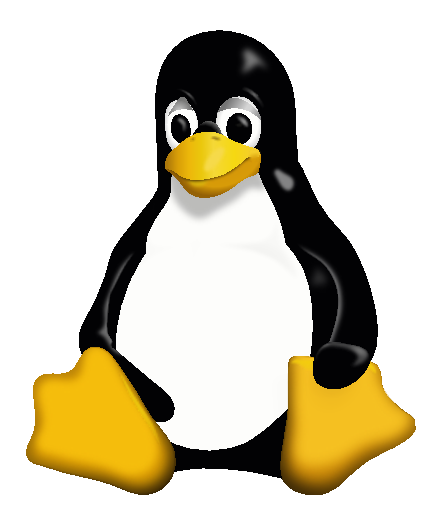
\includegraphics[height=4cm]{Tux.pdf}
\end{minipage}
\hfill
\begin{minipage}[c]{0.64\textwidth}
\setlength{\parskip}{1em}
\begin{lstlisting}[label=includegraphicsbeispiel, style=customlatex]
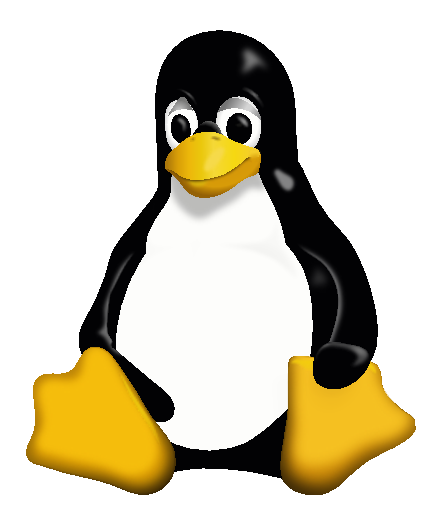
\includegraphics[height=4cm]{Tux.pdf}
\end{lstlisting}
\end{minipage}
\caption{Abbildungen skalieren die Optionen \texttt{height} oder alternativ \texttt{width}}
\label{Beispiel_includegraphics1}
\end{figure}

Soll eine Abbildung genauso breit sein wie das Textfeld, können Autoren das mit \verb!width=\textwidth! realisieren. Das folgende Beispiel würde die Abbildung \verb!bilddatei.pdf! so skalieren, das die Bildbreite der halben Breite des Textes entspricht.

\verb!\includegraphics[width=.5\textwidth]{bilddatei.pdf}!

Alternativ kann auch die Bildbreite fest inklusive einer Maßeinheit 
(siehe Abschnitt~\ref{sec:Massangaben}) definiert sein.

Das Drehen von Bildern ermöglicht der Parameter \verb!angle=!\textsl{Winkel}. 

Im Beispiel in Abbildung~\ref{Beispiel_includegraphics2} ist das Linux-Maskottchen auf die Bildhöhe 3\,cm skaliert und um 270 Grad gedreht.

\begin{figure}[H]
\begin{minipage}[c]{0.34\textwidth}
\setlength{\parskip}{1em}
\centering
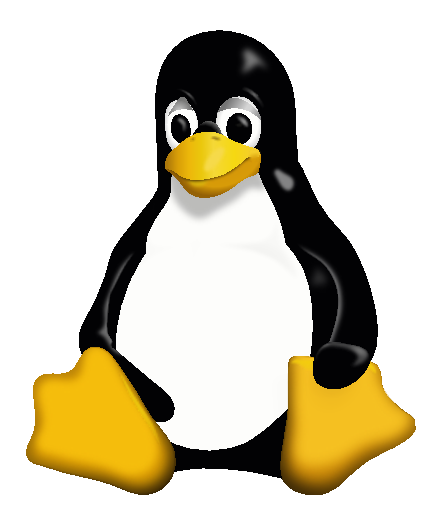
\includegraphics[height=3cm,angle=270]{Tux.pdf}
\end{minipage}
\hfill
\begin{minipage}[c]{0.64\textwidth}
\setlength{\parskip}{1em}
\begin{lstlisting}[label=includegraphicsanglebeispiel, style=customlatex]
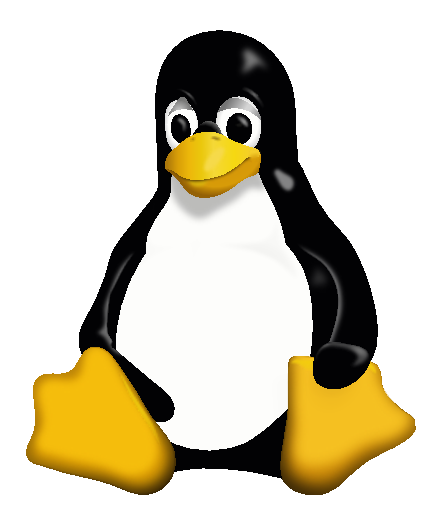
\includegraphics[height=3cm,angle=270]{Tux.pdf}
\end{lstlisting}
\end{minipage}
\caption{Abbildungen drehen ermöglicht die Option \texttt{angle}}
\label{Beispiel_includegraphics2}
\end{figure}

% !!! Hier noch den Abschnitt von Figure einfügen !!!

Meist ist es sinnvoll Abbildungen mit der Umgebung \verb!figure! zu umschließen. Dadurch werden sie zu sogenannten Gleitobjekten. Vorteile von Gleitobjekten sind die automatisierte Positionierung sowie die Möglichkeit Bildunterschriften und Bezeichner zuweisen zu können. Ein mögliches Beispiel ist:

\begin{Verbatim}[frame=single]
\begin{figure}[H]
\includegraphics[width=7cm]{Dateiname}
\caption{Hier ist die Bildunterschrift definiert}
\label{fig:eindeutiger_bezeichner}
\end{figure}
\end{Verbatim}

Ist einer Abbildung mit dem Befehl \verb!\label{!\textsl{Name}\verb!}! ein Bezeichner zugewiesen, kann an jeder beliebigen Stelle im Dokument mit dem Befehl \verb!\ref{!\textsl{Name}\verb!}! darauf verwiesen werden.

Mit dem Befehl \verb!\caption{!\textsl{Bildunterschrift}\verb!}!\index[cmd]{\texttt{\textbackslash caption}} geschieht die Definition der Bildunterschrift. 

\section{Pfade der Bilddateien definieren}

Beim Einbinden einer Abbildung mit dem Befehl \verb!\includegraphics! kann der Pfad zur Bilddatei inklusive des Pfades relativ von der \verb!.tex!-Quelldatei oder absolut von der Wurzel des Dateisystems angegeben sein. Einige Beispiele enthält Tabelle~\ref{Tabelle_Relative_und_Absolute_Pfade}.

\begin{table}[h!tb]
\centering
\caption{Beispiele für relative und absolute Pfade}
\label{Tabelle_Relative_und_Absolute_Pfade}
\begin{tabular}{ccl}
\hline
\textbf{Pfad} & \textbf{Betriebssystem} & \textbf{Beispiel} \\
\hline
relativ & Linux/UNIX   & \texttt{\textbackslash includegraphics[}\textsl{...}\texttt{]\{}\textsl{pfad/zur/bilddatei}\texttt{\}} \\
absolut & Linux/UNIX   & \texttt{\textbackslash includegraphics[}\textsl{...}\texttt{]\{}\textsl{/pfad/zur/bilddatei}\texttt{\}} \\
relativ & Windows & \texttt{\textbackslash includegraphics[}\textsl{...}\texttt{]\{}\textsl{pfad\textbackslash zur\textbackslash bilddatei}\texttt{\}}  \\
absolut & Windows & \texttt{\textbackslash includegraphics[}\textsl{...}\texttt{]\{}\textsl{C:\textbackslash pfad\textbackslash zur\textbackslash bilddatei}\texttt{\}}  \\
\hline
\end{tabular}
\end{table}

Dieses Vorgehen hat den Nachteil, das wenn sich der Pfad zu den eingefügten Bilddateien  einmal ändert, sind an mehreren Stellen im Quelltext Änderungen nötig. Aus diesem Grund ist es sinnvoll, den oder die Pfade zu den verwendeten Bilddateien zentral an einer Stelle in der Präambel der \verb!.tex!-Quelldatei zu definieren. Dieses geschieht mit dem Befehl \verb!\graphicspath!\index[cmd]{\texttt{\textbackslash graphicspath}}. 

\fbox{\texttt{\textbackslash graphicspath\{\{}\textsl{Verzeichnis1/}\texttt{\}\{}\textsl{Verzeichnis2/}\texttt{\}...\{}\textsl{Verzeichnisn/}\texttt{\}\}}}

Jeder als Argument übergebene Pfad (egal ob es sich dabei um einen relativen oder um einen absoluten Pfad handelt), sollte unter Linux mit einem Slash enden und unter Windows mit einem Backslash. Zudem muss jeder Pfad von geschweiften Klammern umschlossen sein.


\chapter{Mathematischer Formelsatz}
\label{KapitelMathematik}
\index{Mathematik}
\index{Formelsatz}

Die Fähigkeiten von \LaTeX, wenn es um den optisch ansprechenden Satz mathematischer Formeln geht, sind einer der am häufigsten genannten Vorzüge dieses Textsatzsystems. Möglicherweise ist diese Eigenschaft auch einer der Gründe für die Popularität von \LaTeX\ im universitären Umfeld und im Verlagswesen.

Zum Formelsatz bietet \LaTeX\ verschiedene Umgebungen für eingebettete Formeln, die auch Textformeln heißen
und für abgesetzte Formeln.

Textformeln befinden sich im fortlaufenden Text. Abgesetzte Formeln hingegen werden
mit einem Zwischenraum über und unter der Formel gesetzt und horizontal zentriert.

\section{Eingebettete Formeln (Textformeln)}
\index{Textformel}
\index{Formel!eingebettete}

Die kompakteste Möglichkeit, eine eingebettete Formel zu realisieren, ist im Quelltext vor und hinter die 
Formel ein \verb!$!-Zeichen zu stellen. 

\fbox{\texttt{\$}\textsl{Formel}\texttt{\$}}

Ein negativer Aspekt dieser Vorgehensweisen ist, dass
beide Begrenzungssymbole identisch und daher zweideutig sind. 
Je nach Struktur des Dokuments wirkt sich das negativ auf die Lesbarkeit des Quelltextes aus.
Eleganter und weniger fehleranfällig ist das
Umschließen der Formel mit den Zeichenketten \verb!\(! und \verb!\)!.

\fbox{\texttt{\textbackslash (}\textsl{Formel}\texttt{\textbackslash )}}


Zusätzlich existiert die Umgebung \verb!math!\index[cmd]{\texttt{math}}, deren Verwendung zum
gleichen Ergebnis führt wie die
Verwendung von \verb!$...$! und \verb!\(...\)!.

\begin{boxedminipage}{\textwidth}
\texttt{\textbackslash
begin\{math\} \\
\textsl{Formel} \\
\textbackslash end\{math\}}
\end{boxedminipage}





\section{Abgesetzte Formeln}
\index{Formel!abgesetzt} 

Auch zur Erzeugung abgesetzter Formeln existieren verschiedene
Möglichkeiten. Eine Möglichkeit ist, den Anfang und 
das Ende der abgesetzten Formel mit \verb!$$! zu kennzeichnen. 
Allerdings gibt es auch hier das Problem, das
beide Begrenzungssymbole identisch und daher zweideutig sind. 


\fbox{\texttt{\$\$}\textsl{Formel}\texttt{\$\$}}

Eine weitere
Möglichkeit ist, den Anfang der Formel mit \verb!\[! und das Ende mit
\verb!\]! zu kennzeichnen.


\fbox{\texttt{\textbackslash [}\textsl{Formel}\texttt{\textbackslash ]}}


Zusätzlich existiert die Umgebung \verb!displaymath!\index[cmd]{\texttt{displaymath}}, 
deren Verwendung zum
gleichen Ergebnis führt wie die
Verwendung von \verb!$$...$$! und \verb!\[...\]!.

\begin{boxedminipage}{\textwidth}
\texttt{\textbackslash
begin\{displaymath\} \\
\textsl{Formel} \\
\textbackslash end\{displaymath\}}
\end{boxedminipage}


Alle bisher vorgestellten Möglichkeiten zum Satz abgesetzter Formeln bewirken, das der \LaTeX-Compiler den aktuellen Absatz  
abbricht und einen vertikalen
Freiraum einfügt. Die abgesetzte 
Formel wird horizontal zentriert 
gesetzt, und nach einem weiteren vertikalen 
Freiraum geht es mit dem Text weiter. Das folgende Beispiel zeigt diese Arbeitsweise:


\begin{minipage}[c]{.48\textwidth}
\setlength{\parskip}{1em}
\begin{displaymath}
(a+b)^2 = a^2 + 2ab + b^2
\end{displaymath}
\end{minipage}
\hfill
\begin{minipage}{.48\textwidth}
\setlength{\parskip}{1em}
\begin{lstlisting}[label=abgesetzteformelnbeispiel, style=customlatex]
\begin{displaymath}
(a+b)^2 = a^2 + 2ab + b^2
\end{displaymath}
\end{lstlisting}
\end{minipage}



Sollen Formeln nummeriert\index{Formel!nummeriert} sein, um im Fließtext einfach darauf Bezug nehmen zu können, 
ist es sinnvoll die abgesetzten Formeln mit der Umgebung
\verb!equation!\index[cmd]{\texttt{equation}-Umgebung} zu erzeugen. In diesem Fall erhält die Formel automatisch eine
eindeutige Nummer.


\begin{boxedminipage}{\textwidth}
\texttt{\textbackslash
begin\{equation\} \\
\textsl{Formel} \\
\textbackslash end\{equation\}}
\end{boxedminipage}


Zum Satz von Gleichungssystemen\index{Gleichungssysteme} bzw. für den Satz mehrerer untereinander angeordneter Formeln
existieren die Umgebungen \verb!eqnarray! und \verb!eqnarray*!\index[cmd]{\texttt{eqnarray}}.
Beide Umgebungen unterscheiden sich nur darin, das bei der Umgebung \verb!eqnarray!
jede Zeile nummeriert wird und bei \verb!eqnarray*! ist das nicht der Fall.

\begin{boxedminipage}{\textwidth}
\texttt{\textbackslash
begin\{eqnarray\} \\
\textsl{Formel} \\
\textbackslash end\{eqnarray\}}
\end{boxedminipage}

\begin{boxedminipage}{\textwidth}
\texttt{\textbackslash
begin\{eqnarray*\} \\
\textsl{Formel} \\
\textbackslash end\{eqnarray*\}}
\end{boxedminipage}


Die Arbeitsweise der beiden Umgebungen 
\verb!eqnarray! und\index[cmd]{\texttt{eqnarray}-Umgebung} 
\verb!eqnarray*!\index[cmd]{\texttt{eqnarray$\ast$}-Umgebung}
ist vergleichbar mit der Arbeitsweise einer Tabelle, die in drei Spalten
unterteilt ist, und deren 
Spaltendefinition \verb!{rcl}! entspricht. 
Das heißt, der Inhalt der ersten Spalte wird rechtsbündig, der Inhalt der 
zweiten Spalte zentriert, und der Inhalt der dritten Spalte wird linksbündig gesetzt. 

Genau wie bei Tabellen sind Spalten mit dem Zeichen \verb!&! voneinander abgegrenzt
und das Ende einer Zeile kennzeichnet der Befehl \verb!\\!.

Der Grund, warum die zweite Spalte zentriert gesetzt wird, ist, dass 
sie für die Aufnahme eines Relationssymbols gedacht ist, wie es bei 
Gleichungssystemen in jeder Zeile verwendet wird. In den meisten Fällen wird es sich um 
das Zeichen \verb!=! handeln.

Die folgende Gleichung wurde mit der Umgebung \verb!eqnarray*! gesetzt:

\begin{eqnarray*}
	P(\neg C \vee D) & = & 1 - P(\neg D \wedge C) \\
	& = & 1 - P(\neg D|C) \cdot P(C) \\
	& = & 1 - P(C) \cdot (1 - P(D|C)) \\
	& = & 1 - P(C) + P(D|C) \cdot P(C) \\		 
	& = & P(\neg C) + P(D|C) \cdot P(C)
\end{eqnarray*}

Der Quelltest zu dieser Gleichung aus dem Fachgebiet der
Wissensverarbeitung wurde mit folgendem Quelltext erzeugt:

\begin{lstlisting}[label=eqnarraybeispiel, style=customlatex]
\begin{eqnarray*}
P(\neg C \vee D) & = & 1 - P(\neg D \wedge C) \\
& = & 1 - P(\neg D|C) \cdot P(C) \\
& = & 1 - P(C) \cdot (1 - P(D|C)) \\
& = & 1 - P(C) + P(D|C) \cdot P(C) \\		 
& = & P(\neg C) + P(D|C) \cdot P(C)
\end{eqnarray*}
\end{lstlisting}


Sollen bei einer Gleichung, die mit der Umgebung \verb!eqnarray! gesetzt wird, einzelne Zeilen 
keine Nummer erhalten, können Autoren dieses in den jeweiligen Zeilen mit dem Befehl Befehl \verb!\nonumber!
anweisen.

\fbox{\texttt{\textbackslash nonumber}}
\index[cmd]{\texttt{\textbackslash nonumber}} 

Der Befehl wird einfach an das Ende jeder Zeile einer 
\verb!eqnarray!-Umgebung geschrieben, die
von der Nummerierung ausgeschlossen sein soll.


\section{Grundlegende mathematische Konstrukte}
\index{Mathematik!Konstrukte} 

Dieser Abschnitt stellt die nötigen Befehle vor, um einige der wichtigsten 
mathematischen Konstrukte realisieren können. 
Dazu gehören Brüche, Wurzeln,
Indizes und Exponenten, Summen und Integrale.




\subsection{Brüche}
\index{Bruch}
\index{Mathematik!Bruch}

Der Satz von Brüchen ist innerhalb eingebetteter und abgesetzter Formeln mit dem Befehl \verb!\frac! möglich.\index[cmd]{\texttt{\textbackslash frac}} 


\fbox{\texttt{\textbackslash frac\{{\textsl Zähler}\}\{{\textsl Nenner}\}}}

Das erste Argument des Befehls enthält den \textsl{Zähler}\index{Zähler} über dem Bruchstrich\index{Bruchstrich} und das zweite Argument den \textsl{Nenner}\index{Nenner} unter dem Bruchstrich (siehe Abbildung~\ref{Beispiel_frac1}). \textsl{Zähler} und\index{Nenner}
\textsl{Nenner} selbst können Formeln von fast beliebiger Komplexität enthalten.

\begin{figure}[H]
\begin{minipage}[c]{.4\textwidth}
\setlength{\parskip}{1em}
\[
  \frac{a}{b} + \frac{c}{d} = 
  \frac{a\cdot d+c\cdot b}{b\cdot d}
\]
\end{minipage}
\hfill
\begin{minipage}{.58\textwidth}
\setlength{\parskip}{1em}
\begin{lstlisting}[label=fracbeispiel, style=customlatex]
\[
  \frac{a}{b} + \frac{c}{d} = 
  \frac{a\cdot d+c\cdot b}{b\cdot d}
\]
\end{lstlisting}
\end{minipage}
\caption{Der Satz von Brüchen geschieht mit dem Befehl \texttt{\textbackslash frac}}
\label{Beispiel_frac1}
\end{figure}

Als eingebettete Formel, unter Verwendung von \verb!$...$!, \verb!\(...\)! oder der Umgebung \verb!math!,  sieht das Beispiel von Abbildung~\ref{Beispiel_frac1} deutlich kompakter aus: \(\frac{a}{b} + \frac{c}{d} = \frac{a\cdot d+c\cdot b}{b\cdot d}\).

\subsection{Indizes und Exponenten}
\index{Index} 
\index{Exponent} 

Das Setzen eines Index geschieht 
mit Hilfe eines Unterstriches 
\verb!_!. Alles, was nach
dem Unterstrich kommt, setzt der \LaTeX-Compiler als Index 
der vorhergegangenen Teilformel. 

\fbox{\texttt{\textunderscore\{}\textsl{Index}\}}

Das Setzen von Exponenten geschieht mit dem Zeichen 
\verb!^!. Das darauf folgende Zeichen 
(oder die darauf folgende Teilformel) 
setzt der \LaTeX-Compiler als Exponent.

\fbox{\texttt{\textasciicircum\{}\textsl{Exponent}\}}

Es verbessert die Lesbarkeit
des Quelltextes, wenn Indizes und Exponenten immer in geschweiften Klammern stehen
und wenn ein Index oder Exponent aus mehr als nur einem einzigen Zeichen besteht, 
müssen diese auch auch zwingend in geschweiften Klammern stehen.

\begin{minipage}[c]{.4\textwidth}
% \setlength{\parskip}{1em}
% \centering
\vspace*{-5mm}
\[ a^{2} + a^{b} - a_{2} + a^{n}_{i} \]
\end{minipage}
\hfill
\begin{minipage}[c]{.58\textwidth}
\setlength{\parskip}{1em}
\verb!\[ a^{2} + a^{b} - a_{2} + a^{n}_{i} \]!
\end{minipage}

\begin{minipage}[c]{.4\textwidth}
% \setlength{\parskip}{1em}
% \centering
\vspace*{-5mm}
\[ (a+b)^{2} = a^{2} + 2ab + b^{2} \]
\end{minipage}
\hfill
\begin{minipage}[c]{.58\textwidth}
\setlength{\parskip}{1em}
\verb!\[ (a+b)^{2} = a^{2} + 2ab + b^{2} \]!
\end{minipage}


Sollen gleichzeitig ein Index und ein Exponenten an ein Zeichen angehängt werden, ist deren
Reihenfolge im Quelltext gleichgültig. Es ist also egal ob \(a^{x}_{y}\) 
so: \verb!\(a^{x}_{y}\)! oder so: \verb!\(a_{y}^{x}\)! realisiert ist. 

\begin{minipage}[c]{.4\textwidth}
% \setlength{\parskip}{1em}
% \centering
\vspace*{-5mm}
\[ a^{n+1} + a^{n_x} \]
\end{minipage}
\hfill
\begin{minipage}[c]{.58\textwidth}
\setlength{\parskip}{1em}
\verb!\[ a^{n+1} + a^{n_x} \]!
\end{minipage}

\begin{minipage}[c]{.4\textwidth}
% \setlength{\parskip}{1em}
% \centering
\vspace*{-5mm}
\[ a^{b^{c^2}} \]
\end{minipage}
\hfill
\begin{minipage}[c]{.58\textwidth}
\setlength{\parskip}{1em}
\verb!\[ a^{b^{c^2}} \]!
\end{minipage}

\begin{minipage}[c]{.4\textwidth}
% \setlength{\parskip}{1em}
% \centering
\vspace*{-5mm}
\[ a^{b^2_i}_{c^{2n-1}_{n+m}} \]
\end{minipage}
\hfill
\begin{minipage}[c]{.58\textwidth}
\setlength{\parskip}{1em}
\verb!\[ a^{b^2_i}_{c^{2n-1}_{n+m}} \]!
\end{minipage}

\begin{minipage}[c]{.4\textwidth}
% \setlength{\parskip}{1em}
% \centering
\vspace*{-5mm}
\[ a^{e^{b_{2}}}_{1} \]
\end{minipage}
\hfill
\begin{minipage}[c]{.58\textwidth}
\setlength{\parskip}{1em}
\verb!\[ a^{e^{b_{2}}}_{1} \]!
\end{minipage}


Da \LaTeX\ die beiden Zeichen \verb!^! oder \verb!_! nur zur Definition von
Indizes und Exponenten in mathematische Umgebungen akzeptiert, können diese 
im Fließtext nicht direkt eingegeben werden. In diesem Fall 
müssen Autoren auf die Befehle \verb!\textasciicircum!\index[cmd]{\texttt{\textbackslash textasciicircum}}
für das Zeichen \verb!^! und \verb!\textunderscore!\index[cmd]{\texttt{\textbackslash textunderscore}}
oder alternativ \verb!\_! für das Zeichen \verb!_! zurückgreifen.


\subsection{Wurzeln}
\index{Wurzel} 


Das Setzen von Wurzeln ermöglicht der Befehl
\verb!sqrt!\index[cmd]{\texttt{\textbackslash sqrt}}.


\fbox{\texttt{\textbackslash sqrt[}\textsl{Ordnung}\texttt{]\{}\textsl{Radikant}\texttt{\}}}

Im ersten Argument ist die \textsl{Ordnung}\index{Ordnung} der Wurzel definiert und im 
zweiten Argument der \textsl{Radikant}\index{Radikant}. Die Ordnung wird immer in eckigen 
Klammern \verb![...]! geschrieben und der 
Radikant muss in geschweiften Klammern stehen \verb!{...}!.



Beide Argumente können fast beliebig komplexe 
Formeln enthalten. 
Die Größe des Wurzelzeichens\index{Wurzelzeichen} wird
legt der \LaTeX-Compiler automatisch fest, wie das Beispiel in Abbildung~\ref{Beispiel_sqrt1} anschaulich zeigt.


\begin{figure}[H]
\begin{minipage}[c]{.5\textwidth}
\setlength{\parskip}{1em}

\[
  \sqrt[1018]{-1}=
  \sqrt{\sqrt{\sqrt{\sqrt{
  \sqrt{\sqrt{\sqrt{\sqrt{
  \sqrt{\sqrt{-1}}}}}}}}}}
\]

\end{minipage}
\hfill
\begin{minipage}{.48\textwidth}
\setlength{\parskip}{1em}
\begin{lstlisting}[label=sqrtbeispiel, style=customlatex]
\[
  \sqrt[1018]{-1}=
  \sqrt{\sqrt{\sqrt{\sqrt{
  \sqrt{\sqrt{\sqrt{\sqrt{
  \sqrt{\sqrt{-1}}}}}}}}}}
\]
\end{lstlisting}
\end{minipage}
\caption{Der Satz von Wurzeln geschieht mit dem Befehl \texttt{\textbackslash sqrt}}
\label{Beispiel_sqrt1}
\end{figure}

Es folgen einige weitere Beispiele, die das Setzen von Wurzeln demonstrieren:

\begin{minipage}[c]{.4\textwidth}
% \setlength{\parskip}{1em}
% \centering
\vspace*{-5mm}
\[ \sqrt{x} + \sqrt{x+y+2} \] 
\end{minipage}
\hfill
\begin{minipage}[c]{.58\textwidth}
\setlength{\parskip}{1em}
\verb!\[ \sqrt{x} + \sqrt{x+y+2} \] !
\end{minipage}

\begin{minipage}[c]{.4\textwidth}
% \setlength{\parskip}{1em}
% \centering
\vspace*{-5mm}
\[ \sqrt[3]{x} + \sqrt[y+1]{x} \]
\end{minipage}
\hfill
\begin{minipage}[c]{.58\textwidth}
\setlength{\parskip}{1em}
\verb!\[ \sqrt[3]{x} + \sqrt[y+1]{x} \] !
\end{minipage}

\begin{minipage}[c]{.4\textwidth}
% \setlength{\parskip}{1em}
% \centering
\vspace*{-5mm}
\[ 1+\sqrt[x]{x+2} \]
\end{minipage}
\hfill
\begin{minipage}[c]{.58\textwidth}
\setlength{\parskip}{1em}
\verb!\[ 1+\sqrt[x]{x+2} \] !
\end{minipage}

\begin{minipage}[c]{.4\textwidth}
% \setlength{\parskip}{1em}
% \centering
\vspace*{-5mm}
\[ \sqrt{x^{9}+\sqrt{\alpha}} \]
\end{minipage}
\hfill
\begin{minipage}[c]{.58\textwidth}
\setlength{\parskip}{1em}
\verb!\[ \sqrt{x^{9}+\sqrt{\alpha}} \] !
\end{minipage}

\begin{minipage}[c]{.4\textwidth}
% \setlength{\parskip}{1em}
% \centering
\vspace*{-5mm}
\[ a^{-r} = \frac{1}{
   \sqrt[\alpha]{a^{p}}} \]
\end{minipage}
\hfill
\begin{minipage}[c]{.58\textwidth}
\setlength{\parskip}{1em}
\verb!\[ a^{-r} = \frac{1}{! \\
\verb!   \sqrt[\alpha]{a^{p}}} \]!
\end{minipage}

\begin{minipage}[c]{.4\textwidth}
% \setlength{\parskip}{1em}
% \centering
\vspace*{-5mm}
\[ \sqrt[13]{\frac{y+b\sin\theta}
   {e^{\imath\vartheta}}} \]
\end{minipage}
\hfill
\begin{minipage}[c]{.58\textwidth}
\setlength{\parskip}{1em}
\verb!\[ \sqrt[13]{\frac{y+b\sin\theta}! \\
\verb!   {e^{\imath\vartheta}}} \]!
\end{minipage}


\subsection{Summen und Integrale}
\index{Summe} 
\index{Integral}
\index{Integralzeichen}
\index{Produktzeichen}

Dieser Abschnitt präsentiert einige 
mathematische Zeichen, darunter unter anderem 
das Summen-, das Integral-, das Produktzeichen und weitere Zeichen. 
Genau wie beim Wurzelzeichen, das im vorherigen Unterabschnitt vorgestellt wurde, 
hängt auch bei den Zeichen in diesem Abschnitt die Größe, in der das betreffende Zeichen gesetzt wird, 
von der verwendeten Umgebung ab. Das heißt konkret, das die Darstellung in
einer eingebetteten Formel kleiner ist als in einer abgesetzten Formel.

Stellvertretend für alle Zeichen in diesem Abschnitt wird an dieser Stelle das
Summenzeichen\index{Summenzeichen} vorgestellt, dessen 
Satz mit dem Befehl \verb!\sum!\index[cmd]{\texttt{\textbackslash sum}} geschieht.

\fbox{\texttt{\textbackslash sum\textunderscore\{}\textsl{unter dem Zeichen}\texttt{\}\textasciicircum\{}\textsl{über dem Zeichen}\}}

Die eingebettete Formel \(\sum_{n=0}^{x}\) wurde mit folgenden 
\LaTeX-Quelltext gesetzt: \verb!\(\sum{n=0}{x}\)!. Als abgesetzte Formel, zum Beispiel mit der Umgebung
\verb!displaymath! oder unter Verwendung von \verb!\[...\]!, sieht der Satz deutlich anders aus:

\begin{minipage}[c]{.4\textwidth}
% \setlength{\parskip}{1em}
% \centering
\[ \sum_{n=0}^{x} \]
\end{minipage}
\hfill
\begin{minipage}[c]{.58\textwidth}
\setlength{\parskip}{1em}
\verb!\[ \sum_{n=0}^{x} \] !
\end{minipage}

Tabelle~\ref{Tabelle_Groessen_mathematischer_Zeichen} enthält eine Übersicht über die 
Größen verschiedener mathematischer Zeichen. Konkret ist in der Tabelle jedes Zeichen in der
Form gesetzt, wie es als eingebettete Formel der Fall ist, und wie es in einer abgesetzten Formel 
der Fall ist. Da abgesetzt Formeln nicht in Tabellen vorkommen dürfen, wurde die gewünschte Darstellung mit dem Befehl 
\verb!\displaystyle!\index[cmd]{\texttt{\textbackslash displaystyle}} erzwungen.

\fbox{\texttt{\textbackslash displaystyle}}






\begin{table}[h!tb]
\centering
\caption{Größenübersicht verschiedener mathematischer Zeichen}
\label{Tabelle_Groessen_mathematischer_Zeichen}       % Give a unique label
\begin{tabular}{ccl}
\hline
abgesetzte Formel & 
eingebettete Formel & 
% \texttt{\textbackslash scriptstyle} & 
% \texttt{\textbackslash scriptscriptstyle} & 
Befehl \\
\hline
\begin{math} \displaystyle \bigcap_{x}^{n} \end{math} &
\begin{math} \bigcap_{x}^{n} \end{math} &
\texttt{\textbackslash bigcap\textunderscore \{x\}\textasciicircum \{n\}} \\
\begin{math} \displaystyle \bigcup_{x}^{n} \end{math} &
\begin{math} \bigcup_{x}^{n} \end{math} &
\texttt{\textbackslash bigcup\textunderscore \{x\}\textasciicircum \{n\}} \\
\begin{math} \displaystyle \bigotimes_{x}^{n} \end{math} &
\begin{math} \bigotimes_{x}^{n} \end{math} &
\texttt{\textbackslash bigotimes\textunderscore \{x\}\textasciicircum \{n\}} \\
\begin{math} \displaystyle \bigoplus_{x}^{n} \end{math} &
\begin{math} \bigoplus_{x}^{n} \end{math} &
\texttt{\textbackslash bigoplus\textunderscore \{x\}\textasciicircum \{n\}} \\
\begin{math} \displaystyle \bigodot_{x}^{n} \end{math} &
\begin{math} \bigodot_{x}^{n} \end{math} &
\texttt{\textbackslash bigodot\textunderscore \{x\}\textasciicircum \{n\}} \\
\begin{math} \displaystyle \bigsqcup_{x}^{n} \end{math} &
\begin{math} \bigsqcup_{x}^{n} \end{math} &
\texttt{\textbackslash bigsqcup\textunderscore \{x\}\textasciicircum \{n\}} \\
\begin{math} \displaystyle \biguplus_{x}^{n} \end{math} &
\begin{math} \biguplus_{x}^{n} \end{math} &
\texttt{\textbackslash biguplus\textunderscore \{x\}\textasciicircum \{n\}} \\
\begin{math} \displaystyle \bigvee_{x}^{n} \end{math} &
\begin{math} \bigvee_{x}^{n} \end{math} &
\texttt{\textbackslash bigvee\textunderscore \{x\}\textasciicircum \{n\}} \\
\begin{math} \displaystyle \bigwedge_{x}^{n} \end{math} &
\begin{math} \bigwedge_{x}^{n} \end{math} &
\texttt{\textbackslash bigwedge\textunderscore \{x\}\textasciicircum \{n\}} \\
\begin{math} \displaystyle \int_{x}^{n} \end{math} &
\begin{math} \int_{x}^{n} \end{math} &
\texttt{\textbackslash int\textunderscore \{x\}\textasciicircum \{n\}} \\
\begin{math} \displaystyle \coprod_{x}^{n} \end{math} &
\begin{math} \coprod_{x}^{n} \end{math} &
\texttt{\textbackslash coprod\textunderscore \{x\}\textasciicircum \{n\}} \\
\begin{math} \displaystyle \oint_{x}^{n} \end{math} &
\begin{math} \oint_{x}^{n} \end{math} &
\texttt{\textbackslash oint\textunderscore \{x\}\textasciicircum \{n\}} \\
\begin{math} \displaystyle \prod_{x}^{n} \end{math} &
\begin{math} \prod_{x}^{n} \end{math} &
\texttt{\textbackslash prod\textunderscore \{x\}\textasciicircum \{n\}} \\
\begin{math} \displaystyle \sqrt[x]{n} \end{math} &
\begin{math} \sqrt[x]{n} \end{math} &
\texttt{\textbackslash sqrt[x]\{n\}} \\
\begin{math} \displaystyle \sum_{x}^{n} \end{math} &
\begin{math} \sum_{x}^{n} \end{math} &
\texttt{\textbackslash sum\textunderscore \{x\}\textasciicircum \{n\}} \\
\hline
\end{tabular}
\end{table}


\subsection{Informationen über oder unter Zeichen positionieren}
\index{Zeichen!positionieren} 

Das Setzten von einzeiligen Informationen in kleinerer Schrift über oder unter einzelnen Zeichen ermöglichen die 
Befehle \verb!\overset!,\index[cmd]{\texttt{\textbackslash overset}}  
\verb!\underset!\index[cmd]{\texttt{\textbackslash underset}}.

\begin{boxedminipage}{\textwidth}
\texttt{\textbackslash overset\{}\textsl{oben}\texttt{\}\{}\textsl{unten}\texttt{\}}
\texttt{\textbackslash underset\{}\textsl{unten}\texttt{\}\{}\textsl{oben}\texttt{\}} \\
\end{boxedminipage}

Der Befehl \verb!\overset! platziert den Inhalt des
Arguments \textsl{oben} über dem Inhalt des Arguments \textsl{unten}
und der Befehl \verb!\underset! platziert den Inhalt des Arguments
\textsl{unten} unter den Inhalt von \textsl{oben}.

Beide Befehle sind Teil des Erweiterungspakets \verb!amsmath! und stehen zur Verfügung, sobald das Paket 
in der Präambel der Quelldatei mit dem Befehl \verb!\usepackage{amsmath}! eingebunden ist.

\begin{minipage}[c]{.4\textwidth}
\setlength{\parskip}{1em}
\[ 
  \overset{y}{X} 
  \qquad
  \underset{y}{X} 
  \qquad  
  \overset{a}{\underset{b}{X}} 
\]
\end{minipage}
\hfill
\begin{minipage}[c]{.58\textwidth}
\setlength{\parskip}{1em}
\begin{lstlisting}[label=oversetundersetbeispiel, style=customlatex]
\[ 
  \overset{y}{X} 
  \qquad
  \underset{y}{X} 
  \qquad  
  \overset{a}{\underset{b}{X}} 
\]
\end{lstlisting}
\end{minipage}


Bei der Bildung einer Summe oder zur Indizierung ist 
es manchmal notwendig, mehrzeilige Angaben 
zu machen. Das Erweiterungspaket \verb!amsmath! enthält für diesen Zweck
den Befehl \verb!\substack!.\index[cmd]{\texttt{\textbackslash substack}}  

\fbox{\texttt{\textbackslash substack\{}\textsl{mehrzeilige Formel}\texttt{\}}}

Das Ende einer Zeile wird im 
Argument \textsl{mehrzeilige Formel}
mit dem Befehl \verb!\\! angewiesen.


\begin{minipage}[c]{.4\textwidth}
\setlength{\parskip}{1em}
\[
  \sum_{\substack{0 \le i \le m \\
                  0 \le j \le m}} P (i,j)
\]
\end{minipage}
\hfill
\begin{minipage}[c]{.58\textwidth}
\setlength{\parskip}{1em}
\begin{lstlisting}[label=substackbeispiel, style=customlatex]
\[
  \sum_{\substack{0 \le i \le m \\
                  0 \le j \le m}} P (i,j)
\]
\end{lstlisting}
\end{minipage}

\section{Mathematische Zeichen und Symbole}

Dieser Abschnitt enthält eine Übersicht über verschiedene 
mathematische Zeichen und Symbole.


\subsection{Griechische Buchstaben im Mathematikmodus} 
\index{Griechische Buchstaben} 
\index{Buchstaben!Griechische} 

Griechische Buchstaben sind in der
Mathematik häufig verwendete Zeichen. Die Erzeugung einiger dieser
Buchstaben geschieht in einer mathematischen Umgebung automatisch, indem \textsl{normale} 
Buchstaben verwendet werden. Für die übrigen Buchstaben existiert eigene Befehle 
(siehe Tabelle~\ref{Tabelle_Griechische_Buchstaben1} und Tabelle~\ref{Tabelle_Griechische_Buchstaben2}). 

\begin{table}[h!tb]
\centering
\caption{Griechische Großbuchstaben}
\label{Tabelle_Griechische_Buchstaben1}       % Give a unique label
\begin{tabular}{clclcl}
\hline
Zeichen & Befehl & Zeichen & Befehl & Zeichen & Befehl \\
\hline
\(A\)      & \texttt{A}                    & \(I\)       & \texttt{I}                     & \(P\)        & \texttt{P}\\
\(B\)      & \texttt{B}                    & \(K\)       & \texttt{K}                     & \(\Sigma\)   & \texttt{\textbackslash Sigma} \\
\(\Gamma\) & \texttt{\textbackslash Gamma} & \(\Lambda\) & \texttt{\textbackslash Lambda} & \(T\)        & \texttt{T}\\
\(\Delta\) & \texttt{\textbackslash Delta} & \(M\)       & \texttt{M}                     & \(\Upsilon\) & \texttt{\textbackslash Upsilon} \\
\(E\)      & \texttt{E}                    & \(N\)       & \texttt{N}                     & \(\Phi\)     & \texttt{\textbackslash Phi}\\
\(Z\)      & \texttt{Z}                    & \(\Xi\)     & \texttt{\textbackslash Xi}     & \(X\)        & \texttt{X}\\
\(H\)      & \texttt{H}                    & \(O\)       & \texttt{O}                     & \(\Psi\)     & \texttt{\textbackslash Psi}\\
\(\Theta\) & \texttt{\textbackslash Theta} & \(\Pi\)     & \texttt{\textbackslash Pi}     & \(\Omega\)   & \texttt{\textbackslash Omega} \\
\hline
\end{tabular}
\end{table}

\begin{table}[h!tb]
\centering
\caption{Griechische Kleinbuchstaben}
\label{Tabelle_Griechische_Buchstaben2}       % Give a unique label
\begin{tabular}{clclcl}
\hline
Zeichen & Befehl & Zeichen & Befehl & Zeichen & Befehl \\
\hline
\(\alpha\) & \texttt{\textbackslash alpha} & 
\(\iota\) & \texttt{\textbackslash iota} &
\(\rho\) & \texttt{\textbackslash rho}\\
\(\beta\) & {\texttt \textbackslash beta} &
\(\kappa\) & \texttt{\textbackslash kappa} &
\(\sigma\) & \texttt{\textbackslash sigma}\\
\(\gamma\) & \texttt{\textbackslash gamma} & 
\(\lambda\) & \texttt{\textbackslash lambda} &
\(\tau\) & \texttt{\textbackslash tau} \\
\(\delta\) & \texttt{\textbackslash delta} &
\(\mu\) & \texttt{\textbackslash mu} &
\(\upsilon\) & \texttt{\textbackslash upsilon} \\
\(\epsilon\) & \texttt{\textbackslash epsilon} & 
\(\nu\) & \texttt{\textbackslash nu} &
\(\phi\) & \texttt{\textbackslash phi} \\
\(\zeta\) & \texttt{\textbackslash zeta} & 
\(\xi\) & \texttt{\textbackslash xi} &
\(\chi\) & \texttt{\textbackslash chi}\\
\(\eta\) & \texttt{\textbackslash eta} & 
\(o\) & \texttt{o} &
\(\psi\) & \texttt{\textbackslash psi} \\
\(\theta\) & \texttt{\textbackslash theta} & 
\(\pi\) & \texttt{\textbackslash pi} &
\(\omega\) & \texttt{\textbackslash omega} \\
\hline
\end{tabular}
\end{table}

Wie in Tabelle~\ref{Tabelle_Griechische_Buchstaben1} und Tabelle~\ref{Tabelle_Griechische_Buchstaben2} zu sehen ist, 
setzt der \LaTeX-Compiler griechischen Großbuchstaben üblicherweise in der Schrift Roman und griechische Kleinbuchstaben in der geneigten Schrift \textit{Italic} (siehe Abschnitt~\ref{AbschnittSchriftfamilienSchriftschnitte}).
Sollen auch Großbuchstaben in geneigter Schrift ausgegeben werden, können Autoren dieses mit dem Befehl 
\verb!\mathnormal!\index[cmd]{\texttt{\textbackslash mathnormal}} anweisen.

\fbox{\texttt{\textbackslash mathnormal\{\textsl{Zeichen}\texttt{\}}}}

Das Argument \verb!Zeichen! enthält die
kursiv zu schreibenden griechischen Großbuchstaben.

\begin{minipage}[c]{.4\textwidth}
\setlength{\parskip}{1em}
\centering
\( \mathnormal{\Gamma\Delta\Theta\Pi} \)
\end{minipage}
\hfill
\begin{minipage}[c]{.58\textwidth}
\setlength{\parskip}{1em}
\begin{lstlisting}[label=mathnormalbeispiel, style=customlatex]
\( \mathnormal{\Gamma\Delta\Theta\Pi} \)
\end{lstlisting}
\end{minipage}

Tabelle~\ref{Tabelle_Griechische_Buchstaben3} zeigt Varianten einiger 
griechischen Kleinbuchstaben, die u.a. als Variablen nützlich sind.


\begin{table}[h!tb]
\centering
\caption{Variierte griechische Kleinbuchstaben}
\label{Tabelle_Griechische_Buchstaben3}       % Give a unique label
\begin{tabular}{clclcl}
\hline
Zeichen & Befehl & Zeichen & Befehl & Zeichen & Befehl \\
\hline
$\varepsilon$ & \texttt{\textbackslash varepsilon} &
$\varpi$ & \texttt{\textbackslash varpi} &
$\varsigma$ & \texttt{\textbackslash varsigma}\\
$\vartheta$ & \texttt{\textbackslash vartheta} &
$\varrho$ & \texttt{\textbackslash varrho} &
$\varphi$ & \texttt{\textbackslash varphi} \\
\hline
\end{tabular}
\index[cmd]{\texttt{\textbackslash varepsilon}}
\index[cmd]{\texttt{\textbackslash varpi}}
\index[cmd]{\texttt{\textbackslash varsigma}}
\index[cmd]{\texttt{\textbackslash vartheta}}
\index[cmd]{\texttt{\textbackslash varrho}}
\index[cmd]{\texttt{\textbackslash varphi}}
\end{table}


\subsection{Kalligrafische Buchstaben}
\index{Buchstaben!Kalligrafische}
\index{Kalligrafie}

Den Satz von $\mathcal{KALLIGRAFISCHEN}$ Buchstaben innerhalb mathematischer Umgebungen ermöglicht der
Befehl \verb!\mathcal!\index[cmd]{\texttt{\textbackslash mathcal}}.


\fbox{\texttt{\textbackslash mathcal\{\textsl{Zeichen}\texttt{\}}}}

Im Gegensatz zu den griechischen
Buchstaben sind die kalligrafischen Buchstaben nur als Großbuchstaben verfügbar.

\begin{minipage}[c]{.4\textwidth}
\setlength{\parskip}{1em}
\centering
\( \mathcal{A,B,C,D,E,F,G} \)
\end{minipage}
\hfill
\begin{minipage}[c]{.58\textwidth}
\setlength{\parskip}{1em}
\begin{lstlisting}[label=mathcalbeispiel, style=customlatex]
\( \mathcal{A,B,C,D,E,F,G} \)
\end{lstlisting}
\end{minipage}

Eine Übersicht über die verfügbaren kalligrafischen Buchstaben
enthält Tabelle~\ref{Tabelle_Kalligrafische_Buchstaben3}.


\begin{table}[h!tb]
\centering
\caption{Kalligrafische Zeichen}
\label{Tabelle_Kalligrafische_Buchstaben3}       % Give a unique label
\begin{tabular}{clclcl}
\hline
Zeichen & Befehl & Zeichen & Befehl & Zeichen & Befehl \\
\hline
\(\mathcal{A}\) & \texttt{\textbackslash mathcal\{A\}} &
\(\mathcal{J}\) & \texttt{\textbackslash mathcal\{J\}} & 
\(\mathcal{S}\) & \texttt{\textbackslash mathcal\{S\}} \\
\(\mathcal{B}\) & \texttt{\textbackslash mathcal\{B\}} & 
\(\mathcal{K}\) & \texttt{\textbackslash mathcal\{K\}} &
\(\mathcal{T}\) & \texttt{\textbackslash mathcal\{T\}} \\
\(\mathcal{C}\) & \texttt{\textbackslash mathcal\{C\}} & 
\(\mathcal{L}\) & \texttt{\textbackslash mathcal\{L\}} &
\(\mathcal{U}\) & \texttt{\textbackslash mathcal\{U\}} \\
\(\mathcal{D}\) & \texttt{\textbackslash mathcal\{D\}} & 
\(\mathcal{M}\) & \texttt{\textbackslash mathcal\{M\}} &
\(\mathcal{V}\) & \texttt{\textbackslash mathcal\{V\}}\\
\(\mathcal{E}\) & \texttt{\textbackslash mathcal\{E\}} & 
\(\mathcal{N}\) & \texttt{\textbackslash mathcal\{N\}} &
\(\mathcal{W}\) & \texttt{\textbackslash mathcal\{W\}}\\
\(\mathcal{F}\) & \texttt{\textbackslash mathcal\{F\}} & 
\(\mathcal{O}\) & \texttt{\textbackslash mathcal\{O\}} &
\(\mathcal{X}\) & \texttt{\textbackslash mathcal\{X\}}\\
\(\mathcal{G}\) & \texttt{\textbackslash mathcal\{G\}} & 
\(\mathcal{P}\) & \texttt{\textbackslash mathcal\{P\}} &
\(\mathcal{Y}\) & \texttt{\textbackslash mathcal\{Y\}}\\
\(\mathcal{H}\) & \texttt{\textbackslash mathcal\{H\}} &
\(\mathcal{Q}\) & \texttt{\textbackslash mathcal\{Q\}} &
\(\mathcal{Z}\) & \texttt{\textbackslash mathcal\{Z\}}\\
\(\mathcal{I}\) & \texttt{\textbackslash mathcal\{I\}} &
\(\mathcal{R}\) & \texttt{\textbackslash mathcal\{R\}} & 
& \\
\hline
\end{tabular}
\end{table}



\subsection{Operationssymbole}
\index{Operationssymbole} 


Werden in der Mathematik zwei Objekte mit jeweils einer bestimmten Größe 
miteinander verknüpft und entsteht dabei ein neues Objekt mit einer bestimmten Größe, dann heißt diese Verknüpfung 
eine \textsl{binäre Operation}.\index{binäre Operationen} Tabelle~\ref{Tabelle_Binaere_Operationssymbole} zeigt eine Auswahl an binären Operationssymbolen.


\begin{table}[h!tb]
\centering
\caption{Binäre Operationssymbole}
\label{Tabelle_Binaere_Operationssymbole}       % Give a unique label
\begin{tabular}{clcl}
\hline
Zeichen & Befehl & Zeichen & Befehl  \\
\hline
$\amalg$ & \texttt{\textbackslash amalg} &
$\ominus$ & \texttt{\textbackslash ominus} \\
$\ast$ & \texttt{\textbackslash ast} &
$\oplus$ & \texttt{\textbackslash oplus} \\
$\bigcirc$ & \texttt{\textbackslash bigcirc} &
$\oslash$ & \texttt{\textbackslash oslash} \\
$\bigtriangledown$ & \texttt{\textbackslash bigtriangledown} &
$\otimes$ & \texttt{\textbackslash otimes} \\
$\bigtriangleup$ & \texttt{\textbackslash bigtriangleup} &
$\pm$ & \texttt{\textbackslash pm} \\
$\Box$ & \texttt{\textbackslash Box$^\ast$} &
$\rhd$ & \texttt{\textbackslash rhd$^\ast$} \\
$\bullet$ & \texttt{\textbackslash bullet} &
$\setminus$ & \texttt{\textbackslash setminus} \\
$\cap$ & \texttt{\textbackslash cap} &
$\sqcap$ & \texttt{\textbackslash sqcap} \\
$\cdot$ & \texttt{\textbackslash cdot} &
$\sqcup$ & \texttt{\textbackslash sqcup} \\
$\circ$ & \texttt{\textbackslash circ} &
$\star$ & \texttt{\textbackslash star} \\
$\cup$ & \texttt{\textbackslash cup} &
$\times$ & \texttt{\textbackslash times} \\
$\dagger$ & \texttt{\textbackslash dagger} &
$\triangleleft$ & \texttt{\textbackslash triangleleft} \\
$\ddagger$ & \texttt{\textbackslash ddagger} &
$\triangleright$ & \texttt{\textbackslash triangleright} \\
$\Diamond$ & \texttt{\textbackslash Diamond$^\ast$} &
$\unlhd$ & \texttt{\textbackslash unlhd$^\ast$} \\
$\diamond$ & \texttt{\textbackslash diamond} &
$\unrhd$ & \texttt{\textbackslash unrhd$^\ast$} \\
$\div$ & \texttt{\textbackslash div} &
$\uplus$ & \texttt{\textbackslash uplus} \\
$\lhd$ & \texttt{\textbackslash lhd$^\ast$} &
$\vee$ & \texttt{\textbackslash vee} \\
$\mp$ & \texttt{\textbackslash mp} &
$\wedge$ & \texttt{\textbackslash wedge} \\
$\odot$ & \texttt{\textbackslash odot} &
$\wr$ & \texttt{\textbackslash wr} \\
\hline
\end{tabular}
\end{table}


Diejenigen binären Operationssymbole in Tabelle~\ref{Tabelle_Binaere_Operationssymbole}, die mit einem $^\ast$ gekennzeichnet sind,
erfordern das Einbinden des \verb!latexsym!-Pakets mit dem Befehl 
\verb!\usepackage{latexsym}! in der Präambel der Quelldatei.


\subsection{Vergleichssymbole}
\index{Vergleichssymbole} 

Tabelle~\ref{Tabelle_Vergleichssymbole} zeigt eine Auswahl an 
Vergleichssymbolen.

\begin{table}[h!tb]
\centering
\caption{Vergleichssymbole}
\label{Tabelle_Vergleichssymbole}       % Give a unique label
\begin{tabular}{clcl}
\hline
Zeichen & Befehl & Zeichen & Befehl  \\
\hline
$<$ & \texttt{<} &
$\ni$ & \texttt{\textbackslash ni} \\
$>$ & \texttt{>} &
$\parallel$ & \texttt{\textbackslash parallel} oder \texttt{\textbackslash$|$} \\
$=$ & \texttt{=} &
$\perp$ & \texttt{\textbackslash perp} \\
$\approx$ & \texttt{\textbackslash approx} & 
$\prec$ & \texttt{\textbackslash prec} \\
$\asymp$ & \texttt{\textbackslash asymp} & 
$\preceq$ & \texttt{\textbackslash preceq} \\
$\bowtie$ & \texttt{\textbackslash bowtie} & 
$\propto$ & \texttt{\textbackslash propto} \\ 
$\cong$ & \texttt{\textbackslash cong} &
$\sim$ & \texttt{\textbackslash sim} \\
$\dashv$ & \texttt{\textbackslash dashv} & 
$\smile$ & \texttt{\textbackslash smile} \\
$\doteq$ & \texttt{\textbackslash doteq} & 
$\sqsubseteq$ & \texttt{\textbackslash sqsubseteq} \\
$\equiv$ & \texttt{\textbackslash equiv} & 
$\sqsupseteq$ & \texttt{\textbackslash sqsupseteq} \\
$\frown$ & \texttt{\textbackslash frown} & 
$\subset$ & \texttt{\textbackslash subset} \\  
$\geq$ & \texttt{\textbackslash ge} oder \texttt{\textbackslash geq} &
$\subseteq$ & \texttt{\textbackslash subseteq} \\
$\gg$ & \texttt{\textbackslash gg} & 
$\succ$ & \texttt{\textbackslash succ} \\
$\in$ & \texttt{\textbackslash in} & 
$\succeq$ & \texttt{\textbackslash succeq} \\
$\le$ & \texttt{\textbackslash le} oder \texttt{\textbackslash leq} & 
$\supset$ & \texttt{\textbackslash supset} \\
$\ll$ & \texttt{\textbackslash ll} & 
$\supseteq$ & \texttt{\textbackslash supseteq} \\
$\mid$ & \texttt{\textbackslash mid} oder \texttt{$|$} &
$\simeq$ & \texttt{\textbackslash simeq} \\
$\models$ & \texttt{\textbackslash models} & 
$\vdash$ & \texttt{\textbackslash vdash} \\
\hline
\end{tabular}
\end{table}


Die umgekehrte, also verneinende
Bedeutung eines solchen Vergleichssymbols wird
in der Mathematik durch ein Durchstreichen des betreffenden Symbols mit einem Schrägstrich (\textsl{Slash})
\verb!/! gekennzeichnet. So ist die Negation von \(=\) (\textsl{gleich}) 
beispielsweise \(\neq\) (\textsl{ungleich}).
Die meisten Negationen können durch Voranstellen eines 
\verb!\not!
\index[cmd]{\texttt{\textbackslash not}} erzeugt werden. Für einige wenige existiert ein eigener,
spezieller Befehl (z.B. \verb!\ne! für \(\ne\) oder 
\verb!\notin!
\index[cmd]{\texttt{\textbackslash notin}} für \(\notin\)).

Tabelle~\ref{Tabelle_NegierteVergleichssymbole} zeigt eine Auswahl an
Negationen von Vergleichssymbolen.


\begin{table}[h!tb]
\centering
\caption{Negierte Vergleichssymbole}
\label{Tabelle_NegierteVergleichssymbole}       % Give a unique label
\begin{tabular}{clcl}
\hline
Zeichen & Befehl & Zeichen & Befehl  \\
\hline
$\not<$ & \texttt{\textbackslash not<} & 
$\not\parallel$ & \texttt{\textbackslash not\textbackslash parallel}\\
$\not>$ & \texttt{\textbackslash not>} & 
$\not\perp$ & \texttt{\textbackslash not\textbackslash perp} \\
$\not=$ & \texttt{\textbackslash not=} oder \texttt{\textbackslash neq} oder \texttt{\textbackslash ne}&
$\not\prec$ & \texttt{\textbackslash not\textbackslash prec} \\
$\not\approx$ & \texttt{\textbackslash not\textbackslash approx} & 
$\not\preceq$ & \texttt{\textbackslash not\textbackslash preceq} \\
$\not\asymp$ & \texttt{\textbackslash not\textbackslash asymp} & 
$\not\propto$ & \texttt{\textbackslash not\textbackslash propto} \\
$\not\bowtie$ & \texttt{\textbackslash not\textbackslash bowtie} & 
$\not\sim$ & \texttt{\textbackslash not\textbackslash sim} \\
$\not\cong$ & \texttt{\textbackslash not\textbackslash cong} & 
$\not\simeq$ & \texttt{\textbackslash not\textbackslash simeq} \\
$\not\dashv$ & \texttt{\textbackslash not\textbackslash dashv} & 
$\not\smile$ & \texttt{\textbackslash not\textbackslash smile} \\
$\not\doteq$ & \texttt{\textbackslash not\textbackslash doteq} & 
$\not\sqsubset$ & \texttt{\textbackslash not\textbackslash sqsubset$^\ast$} \\
$\not\equiv$ & \texttt{\textbackslash not\textbackslash equiv} &
$\not\sqsubseteq$ & \texttt{\textbackslash not\textbackslash sqsubseteq} \\
$\not\frown$ & \texttt{\textbackslash not\textbackslash frown} & 
$\not\sqsupset$ & \texttt{\textbackslash not\textbackslash sqsupset$^\ast$} \\
$\not\geq$ & \texttt{\textbackslash not\textbackslash ge} oder \texttt{\textbackslash not\textbackslash geq} & 
$\not\sqsupseteq$ & \texttt{\textbackslash not\textbackslash sqsupseteq} \\
$\not\gg$ & \texttt{\textbackslash not\textbackslash gg} & 
$\not\subset$ & \texttt{\textbackslash not\textbackslash subset} \\
$\notin$ & \texttt{\textbackslash notin} &
$\not\in$ & \texttt{\textbackslash not\textbackslash in} \\
$\not\subseteq$ & \texttt{\textbackslash not\textbackslash subseteq} &
$\not\Join$ & \texttt{\textbackslash not\textbackslash Join$^\ast$} \\
$\not\succ$ & \texttt{\textbackslash not\textbackslash succ} &
$\not\le$ & \texttt{\textbackslash not\textbackslash le} oder \texttt{\textbackslash not\textbackslash leq} \\
$\not\succeq$ & \texttt{\textbackslash not\textbackslash succeq} &
$\not\ll$ & \texttt{\textbackslash not\textbackslash ll} \\
$\not\supset$ & \texttt{\textbackslash not\textbackslash supset} &
$\not\mid$ & \texttt{\textbackslash not\textbackslash mid} \\
$\not\supseteq$ & \texttt{\textbackslash not\textbackslash supseteq} &
$\not\models$ & \texttt{\textbackslash not\textbackslash models} \\
$\not\vdash$ & \texttt{\textbackslash not\textbackslash vdash} &
$\not\ni$ & \texttt{\textbackslash not\textbackslash ni} \\
\hline
\end{tabular}
\end{table}

Diejenigen Symbole in Tabelle~\ref{Tabelle_Zusaetzliche_Vergleichssymbole}, die mit einem $^\ast$ markiert sind, sind nur nach einer
Einbindung des Erweiterungspakets \texttt{latexsym} verfügbar.

Einige zusätzliche Vergleichssymbole (siehe Tabelle~\ref{Tabelle_Zusaetzliche_Vergleichssymbole}) 
bietet das Erweiterungspaket \verb!amssymb!, 
das mit dem Befehl \verb!\usepackage{amssymb}! in der Präambel der Quelldatei eingebunden wird.

\begin{table}[h!tb]
\centering
\caption{Zusätzliche Vergleichssymbole}
\label{Tabelle_Zusaetzliche_Vergleichssymbole}       % Give a unique label
\begin{tabular}{clcl}
\hline
Zeichen & Befehl & Zeichen & Befehl  \\
\hline
$\backepsilon$ & \texttt{\textbackslash backepsilon} &
$\precsim$ & \texttt{\textbackslash precsim} \\
$\backsimeq$ & \texttt{\textbackslash backsimeq} &
$\risingdotseq$ & \texttt{\textbackslash risingdotseq} \\
$\Bumpeq$ & \texttt{\textbackslash Bumpeq} &
$\shortparallel$ & \texttt{\textbackslash shortparallel} \\
$\circeq$ & \texttt{\textbackslash circeq} &
$\smallsmile$ & \texttt{\textbackslash smallsmile} \\
$\eqslantgtr$ & \texttt{\textbackslash eqslantgtr} &
$\sqsubset$ & \texttt{\textbackslash sqsubset} \\
$\gtrdot$ & \texttt{\textbackslash gtrdot} &
$\sqsupset$ & \texttt{\textbackslash sqsupset} \\
$\gtreqless$ & \texttt{\textbackslash gtreqless} &
$\succsim$ & \texttt{\textbackslash succsim} \\
$\Join$ & \texttt{\textbackslash Join} &
$\thickapprox$ & \texttt{\textbackslash thickapprox} \\
$\leqq$ & \texttt{\textbackslash leqq} &
$\trianglelefteq$ & \texttt{\textbackslash trianglelefteq} \\
$\lessdot$ & \texttt{\textbackslash lessdot} &
$\trianglerighteq$ & \texttt{\textbackslash trianglerighteq} \\
$\lesseqgtr$ & \texttt{\textbackslash lesseqgtr} &
$\varpropto$ & \texttt{\textbackslash varpropto} \\
$\lesssim$ & \texttt{\textbackslash lesssim} & & \\
\hline
\end{tabular}
\end{table}


\subsection{Pfeile und Zeiger}
\index{Pfeil}
\index{Zeiger}

Tabelle~\ref{Tabelle_Pfeile} zeigt eine Auswahl an Pfeilen. 
Diejenigen Symbole, die mit einem $^\ast$ markiert sind, sind nur nach einer
Einbindung des Erweiterungspakets \texttt{latexsym} verfügbar.

\begin{table}[h!tb]
\centering
\caption{Pfeile}
\label{Tabelle_Pfeile}       % Give a unique label
\begin{tabular}{clcl}
\hline
Zeichen & Befehl & Zeichen & Befehl  \\
\hline
$\downarrow$ & \texttt{\textbackslash downarrow} & 
$\longrightarrow$ & \texttt{\textbackslash longrightarrow}\\
$\Downarrow$ & \texttt{\textbackslash Downarrow} & 
$\Longrightarrow$ & \texttt{\textbackslash Longrightarrow}\\
$\hookleftarrow$ & \texttt{\textbackslash hookleftarrow} & 
$\mapsto$ & \texttt{\textbackslash mapsto} \\
$\hookrightarrow$ & \texttt{\textbackslash hookrightarrow} &  
$\nearrow$ & \texttt{\textbackslash nearrow} \\
$\leadsto$ & \texttt{\textbackslash leadsto$^\ast$} &  
$\nwarrow$ & \texttt{\textbackslash nwarrow} \\
$\leftarrow$ & \texttt{\textbackslash leftarrow} oder \texttt{\textbackslash gets}& 
$\rightarrow$ & \texttt{\textbackslash rightarrow} oder \texttt{\textbackslash to}\\
$\Leftarrow$ & \texttt{\textbackslash Leftarrow} & 
$\Rightarrow$ & \texttt{\textbackslash Rightarrow} \\
$\leftharpoondown$ & \texttt{\textbackslash leftharpoondown} & 
$\rightharpoondown$ & \texttt{\textbackslash rightharpoondown} \\
$\leftharpoonup$ & \texttt{\textbackslash leftharpoonup} & 
$\rightharpoonup$ & \texttt{\textbackslash rightharpoonup} \\
$\leftrightarrow$ & \texttt{\textbackslash leftrightarrow} & 
$\rightleftharpoons$ & \texttt{\textbackslash rightleftharpoons} \\
$\Leftrightarrow$ & \texttt{\textbackslash Leftrightarrow} & 
$\searrow$ & \texttt{\textbackslash searrow} \\
$\longleftarrow$ & \texttt{\textbackslash longleftarrow} & 
$\swarrow$ & \texttt{\textbackslash swarrow} \\
$\Longleftarrow$ & \texttt{\textbackslash Longleftarrow} & 
$\uparrow$ & \texttt{\textbackslash uparrow} \\
$\longleftrightarrow$ & \texttt{\textbackslash longleftrightarrow} & 
$\Uparrow$ & \texttt{\textbackslash Uparrow} \\
$\Longleftrightarrow$ & \texttt{\textbackslash Longleftrightarrow} & 
$\updownarrow$ & \texttt{\textbackslash updownarrow} \\
$\longmapsto$ & \texttt{\textbackslash longmapsto}& 
$\Updownarrow$ & \texttt{\textbackslash Updownarrow} \\
\hline
\end{tabular}
\end{table}


Es existieren zwei Möglichkeiten, um den Doppelpfeil $\Longleftrightarrow$ zu erzeugen.
Eine Möglichkeit, ist die Verwendung des aus Tabelle~\ref{Tabelle_Pfeile} bekannten Befehls
\verb!\Longleftrightarrow!. Eine alternative Möglichkeit ist die Verwendung des Befehls
\verb!\iff!. Allerdings unterscheiden sich beide
Befehle im Zwischenraum, den \LaTeX\ vor und hinter dem Pfeil einfügt.
Bei \verb!\Longleftrightarrow! $(\Longleftrightarrow)$
ist der Zwischenraum etwas kleiner als bei \verb!\iff! 

Neben den in Tabelle~\ref{Tabelle_Pfeile} vorgestellten Pfeilen, 
bietet das Erweiterungspaket \texttt{amsmath} zahlreiche
Pfeile und Zeiger. Eine Übersicht enthält Tabelle~\ref{Tabelle_Pfeile2}

\begin{table}[h!tb]
\centering
\caption{Pfeile und Zeiger}
\label{Tabelle_Pfeile2}       % Give a unique label
\begin{tabular}{clcl}
\hline
Zeichen & Befehl & Zeichen & Befehl  \\
\hline
$\circlearrowleft$ & \texttt{\textbackslash circlearrowleft} & 
$\looparrowleft$ & \texttt{\textbackslash looparrowleft} \\
$\circlearrowright$ & \texttt{\textbackslash circlearrowright} &
$\Lsh$ & \texttt{\textbackslash Lsh} \\
$\curvearrowleft$ & \texttt{\textbackslash curvearrowleft} &
$\multimap$ & \texttt{\textbackslash multimap} \\
$\curvearrowright$ & \texttt{\textbackslash curvearrowright} &
$\rightarrowtail$ & \texttt{\textbackslash rightarrowtail} \\
$\dashleftarrow$ & \texttt{\textbackslash dashleftarrow} &
$\rightleftarrows$ & \texttt{\textbackslash rightleftarrows} \\
$\dashrightarrow$ & \texttt{\textbackslash dashrightarrow} &
$\rightleftharpoons$ & \texttt{\textbackslash rightleftharpoons} \\
$\downdownarrows$ & \texttt{\textbackslash downdownarrows} &
$\rightrightarrows$ & \texttt{\textbackslash rightrightarrows} \\
$\downharpoonleft$ & \texttt{\textbackslash downharpoonleft} &
$\rightsquigarrow$ & \texttt{\textbackslash rightsquigarrow} \\
$\downharpoonright$ & \texttt{\textbackslash downharpoonright} &
$\Rrightarrow$ & \texttt{\textbackslash Rrightarrow} \\
$\leftarrowtail$ & \texttt{\textbackslash leftarrowtail} &
$\Rsh$ & \texttt{\textbackslash Rsh} \\
$\leftleftarrows$ & \texttt{\textbackslash leftleftarrows} &
$\twoheadleftarrow$ & \texttt{\textbackslash twoheadleftarrow} \\
$\leftrightarrows$ & \texttt{\textbackslash leftrightarrows} &
$\twoheadrightarrow$ & \texttt{\textbackslash twoheadrightarrow} \\
$\leftrightharpoons$ & \texttt{\textbackslash leftrightharpoons} &
$\upuparrows$ & \texttt{\textbackslash upuparrows} \\
$\leftrightsquigarrow$ & \texttt{\textbackslash leftrightsquigarrow} &
$\upharpoonleft$ & \texttt{\textbackslash upharpoonleft} \\
$\Lleftarrow$ & \texttt{\textbackslash Lleftarrow} &
$\upharpoonright$ & \texttt{\textbackslash upharpoonright} \\
\hline
\end{tabular}
\end{table}

Zusätzlich stellt das Erweiterungspaket \verb!amsmath! noch einige negierte (durchgestrichene) 
Pfeile bereit. Eine Übersicht enthält Tabelle~\ref{Tabelle_Negierte_Pfeile}.

\begin{table}[h!tb]
\centering
\caption{Negierte Pfeile}
\label{Tabelle_Negierte_Pfeile}       % Give a unique label
\begin{tabular}{clcl}
\hline
Zeichen & Befehl & Zeichen & Befehl \\
$\nleftarrow$ & \texttt{\textbackslash nleftarrow} & 
$\nLeftarrow$ & \texttt{\textbackslash nLeftarrow} \\
$\nleftrightarrow$ & \texttt{\textbackslash nleftrightarrow} &
$\nLeftrightarrow$ & \texttt{\textbackslash nLeftrightarrow} \\
$\nrightarrow$ & \texttt{\textbackslash nrightarrow} &
$\nRightarrow$ & \texttt{\textbackslash nRightarrow} \\
\hline
\end{tabular}
\end{table}


\subsection{Sonstige mathematische Zeichen}

Tabelle~\ref{Tabelle_Sonstige_Zeichen1} präsentiert weitere
Symbole aller Art, die dem Bereich der mathematischen Zeichen zugeordnet werden können. Einige dieser Zeichen 
sind Teil des Erweiterungspakets \verb!amsmath!.

\begin{table}[h!tb]
\centering
\caption{Sonstige mathematische Zeichen}
\label{Tabelle_Sonstige_Zeichen1}       % Give a unique label
\begin{tabular}{clclcl}
\hline
Zeichen & Befehl & Zeichen & Befehl  \\
\hline
$\aleph$ & \texttt{\textbackslash aleph} & 
$\flat$ & \texttt{\textbackslash flat} \\
$\neg$ & \texttt{\textbackslash neg} &
$\angle$ & \texttt{\textbackslash angle} \\
$\forall$ & \texttt{\textbackslash forall} &
$\partial$ & \texttt{\textbackslash partial}\\
$\backslash$ & \texttt{\textbackslash backslash} & 
$\hbar$ & \texttt{\textbackslash hbar} \\
$\prime$ & \texttt{\textbackslash prime} &
$\bot$ & \texttt{\textbackslash bot} \\
$\heartsuit$ & \texttt{\textbackslash heartsuit} & 
$\Re$ & \texttt{\textbackslash Re}\\
$\clubsuit$ & \texttt{\textbackslash clubsuit} & 
$\imath$ & \texttt{\textbackslash imath} \\
$\spadesuit$ & \texttt{\textbackslash spadesuit} &
$\diamondsuit$ & \texttt{\textbackslash diamondsuit} \\
$\infty$ & \texttt{\textbackslash infty} &
$\surd$ & \texttt{\textbackslash surd}\\
$\ell$ & \texttt{\textbackslash ell} & 
$\jmath$ & \texttt{\textbackslash diamondsuit} \\
$\top$ & \texttt{\textbackslash top} &
$\emptyset$ & \texttt{\textbackslash emptyset} \\
$\nabla$ & \texttt{\textbackslash nabla} &
$\triangle$ & \texttt{\textbackslash triangle}\\
$\exists$ & \texttt{\textbackslash exists} & 
$\natural$ & \texttt{\textbackslash natural} \\
$\wp$ & \texttt{\textbackslash wp} &
$\Im$ & \texttt{\textbackslash Im} \\ 
$\sharp$ & \texttt{\textbackslash sharp}&
$\|$ & \texttt{\textbackslash |}\\
$\backprime$ & \texttt{\textbackslash backprime} & 
$\Diamond$ & \texttt{\textbackslash Diamond} oder \texttt{\textbackslash lozenge} \\
$\Bbbk$ & \texttt{\textbackslash Bbbk} &
$\eth$ & \texttt{\textbackslash eth} \\
$\bigstar$ & \texttt{\textbackslash bigstar} &
$\Finv$ & \texttt{\textbackslash Finv} \\
$\blacksquare$ & \texttt{\textbackslash blacksquare} & 
$\Game$ & \texttt{\textbackslash Game} \\
$\blacklozenge$ & \texttt{\textbackslash blacklozenge} &
$\hslash$ & \texttt{\textbackslash hslash} \\
$\blacktriangle$ & \texttt{\textbackslash blacktriangle} &
$\measuredangle$ & \texttt{\textbackslash measuredangle} \\
$\blacktriangledown$ & \texttt{\textbackslash blacktriangledown}&
$\mho$ & \texttt{\textbackslash mho} \\
$\Box$ & \texttt{\textbackslash Box} oder \texttt{\textbackslash square}&
$\nexists$ & \texttt{\textbackslash nexists} \\
$\circledS$ & \texttt{\textbackslash circledS} &
$\sphericalangle$ & \texttt{\textbackslash sphericalangle}\\
$\complement$ & \texttt{\textbackslash complement} &
$\triangledown$ & \texttt{\textbackslash triangledown} \\
$\diagdown$ & \texttt{\textbackslash diagdown} &
$\varnothing$ & \texttt{\textbackslash varnothing} \\
$\diagup$ & \texttt{\textbackslash diagup} &
$\vartriangle$ & \texttt{\textbackslash vartriangle} \\ 
\hline
\end{tabular}
\end{table}

\subsection{Mathematische Funktionen}

In der Literatur werden mathematische Funktionen üblicherweise nicht -- wie
die Namen von Variablen -- kursiv geschrieben, sondern mit aufrechter Roman-Schrift gesetzt. Eine Übersicht über 
mathematische
Funktionen und deren Befehl zeigt Tabelle~\ref{Tabelle_Mathematische_Funktionen}.


\begin{table}[h!tb]
\centering
\caption{Mathematische Funktionen}
\label{Tabelle_Mathematische_Funktionen}       % Give a unique label
\begin{tabular}{clclcl}
\hline
Zeichen & Befehl & Zeichen & Befehl & Zeichen & Befehl \\
\hline
$\arccos$ & \texttt{\textbackslash arccos} & 
$\exp$ & \texttt{\textbackslash exp} & 
$\max$ & \texttt{\textbackslash max} \\
$\arcsin$  & \texttt{\textbackslash arcsin} & 
$\gcd$ & \texttt{\textbackslash gcd} & 
$\min$ & \texttt{\textbackslash min} \\
$\arctan$ & \texttt{\textbackslash arctan} & 
$\hom$ & \texttt{\textbackslash hom} & 
$\bmod$ & \texttt{\textbackslash bmod} \\
$\arg$ & \texttt{\textbackslash arg} & 
$\inf$ & \texttt{\textbackslash inf} & 
$\mod$ & \texttt{\textbackslash mod} \\
$\cos$ & \texttt{\textbackslash cos} & 
$\ker$ & \texttt{\textbackslash ker} & 
$\Pr$ & \texttt{\textbackslash Pr} \\
$\cosh$ & \texttt{\textbackslash cosh} & 
$\lg$ & \texttt{\textbackslash lg} & 
$\sec$ & \texttt{\textbackslash sec} \\
$\cot$ & \texttt{\textbackslash cot} & 
$\lim$ & \texttt{\textbackslash lim} & 
$\sin$ & \texttt{\textbackslash sin} \\
$\coth$ & \texttt{\textbackslash coth} & 
$\liminf$ & \texttt{\textbackslash liminf} & 
$\sinh$ & \texttt{\textbackslash sinh} \\
$\csc$ & \texttt{\textbackslash csc} &
$\limsup$ & \texttt{\textbackslash limsup} & 
$\sup$ & \texttt{\textbackslash sup} \\
$\deg$ & \texttt{\textbackslash deg} & 
$\ln$ & \texttt{\textbackslash ln} & 
$\tan$ & \texttt{\textbackslash tan} \\
$\det$ & \texttt{\textbackslash det} & 
$\log$ & \texttt{\textbackslash log} & 
$\tanh$ & \texttt{\textbackslash tanh} \\
$\dim$ & \texttt{\textbackslash dim} & & & & \\
\hline
\end{tabular}
\index[cmd]{\texttt{\textbackslash arccos}}
\index[cmd]{\texttt{\textbackslash exp}}
\index[cmd]{\texttt{\textbackslash max}}
\index[cmd]{\texttt{\textbackslash arcsin}} 
\index[cmd]{\texttt{\textbackslash gcd}}
\index[cmd]{\texttt{\textbackslash min}}
\index[cmd]{\texttt{\textbackslash arctan}}
\index[cmd]{\texttt{\textbackslash hom}}
\index[cmd]{\texttt{\textbackslash bmod}}
\index[cmd]{\texttt{\textbackslash arg}}
\index[cmd]{\texttt{\textbackslash inf}}
\index[cmd]{\texttt{\textbackslash mod}}
\index[cmd]{\texttt{\textbackslash cos}}
\index[cmd]{\texttt{\textbackslash ker}}
\index[cmd]{\texttt{\textbackslash Pr}}
\index[cmd]{\texttt{\textbackslash cosh}}
\index[cmd]{\texttt{\textbackslash lg}}
\index[cmd]{\texttt{\textbackslash sec}}
\index[cmd]{\texttt{\textbackslash cot}}
\index[cmd]{\texttt{\textbackslash lim}}
\index[cmd]{\texttt{\textbackslash sin}}
\index[cmd]{\texttt{\textbackslash coth}}
\index[cmd]{\texttt{\textbackslash liminf}}
\index[cmd]{\texttt{\textbackslash sinh}}
\index[cmd]{\texttt{\textbackslash csc}}
\index[cmd]{\texttt{\textbackslash limsup}} 
\index[cmd]{\texttt{\textbackslash sup}}
\index[cmd]{\texttt{\textbackslash deg}}
\index[cmd]{\texttt{\textbackslash ln}} 
\index[cmd]{\texttt{\textbackslash tan}}
\index[cmd]{\texttt{\textbackslash det}}
\index[cmd]{\texttt{\textbackslash log}}
\index[cmd]{\texttt{\textbackslash tanh}}
\index[cmd]{\texttt{\textbackslash dim}}
\end{table}

Der Eintrag $\gcd$ in Tabelle~\ref{Tabelle_Mathematische_Funktionen} entspricht dem 
deutschen ggT (größter gemeinsamer Teiler) und das $\mod$ nach 
rechts eingezogen ist, ist kein Druckfehler, sondern eine Eigenheit des \LaTeX-Compilers.


\subsection{Akzente in Formeln}


Auch in einer mathematischen Umgebung ist es 
möglich, Akzente zu verwenden. Die in Tabelle~\ref{Tabelle_Akzente_Formeln} 
gezeigten Akzente unterscheiden sich von denen im Fließtext.


\begin{table}[h!tb]
\centering
\caption{Akzente in Formeln}
\label{Tabelle_Akzente_Formeln}       % Give a unique label
\begin{tabular}{clclcl}
\hline
Zeichen & Befehl & Zeichen & Befehl & Zeichen & Befehl \\
\hline
$\acute{a}$ & \texttt{\textbackslash acute\{a\}} & 
$\dot{a}$ & \texttt{\textbackslash dot\{a\}} &
$\hat{a}$ & \texttt{\textbackslash hat\{a\}} \\
$\bar{a}$ & \texttt{\textbackslash bar\{a\}} &
$\ddot{a}$ & \texttt{\textbackslash ddot\{a\}} &
$\tilde{a}$ & \texttt{\textbackslash tilde\{a\}} \\
$\breve{a}$ & \texttt{\textbackslash breve\{a\}} &
$\grave{a}$ & \texttt{\textbackslash grave\{a\}} &
$\vec{a}$ & \texttt{\textbackslash vec\{a\}} \\
$\check{a}$ & \texttt{\textbackslash check\{a\}} &
  & \\
\hline
\end{tabular}
\index[cmd]{\texttt{\textbackslash acute}}
\index[cmd]{\texttt{\textbackslash dot}}
\index[cmd]{\texttt{\textbackslash har}}
\index[cmd]{\texttt{\textbackslash bar}}
\index[cmd]{\texttt{\textbackslash ddot}}
\index[cmd]{\texttt{\textbackslash tilde}}
\index[cmd]{\texttt{\textbackslash breve}}
\index[cmd]{\texttt{\textbackslash grave}}
\index[cmd]{\texttt{\textbackslash vec}}
\index[cmd]{\texttt{\textbackslash check}}
\end{table}

Doppelakzente sind mit den in Tabelle~\ref{Tabelle_Akzente_Formeln} gezeigten
Befehlen auch realisierbar, wie Tabelle~\ref{Tabelle_Doppelakzente_Formeln} zeigt.


\begin{table}[h!tb]
\centering
\caption{Doppelakzente in Formeln}
\label{Tabelle_Doppelakzente_Formeln}       % Give a unique label
\begin{tabular}{clcl}
\hline
Zeichen & Befehl & Zeichen & Befehl  \\
\hline
$\acute{\acute{a}}$ & \texttt{\textbackslash acute\{\textbackslash acute\{a\}\}} & 
$\ddot{\ddot{a}}$ & \texttt{\textbackslash ddot\{\textbackslash ddot\{a\}\}} \\
$\bar{\bar{a}}$ & \texttt{\textbackslash bar\{\textbackslash bar\{a\}\}} &
$\grave{\grave {a}}$ & \texttt{\textbackslash grave\{\textbackslash grave\{a\}\}} \\
$\breve{\breve {a}}$ & \texttt{\textbackslash breve\{\textbackslash breve\{a\}\}} &
$\hat{\hat {a}}$ & \texttt{\textbackslash hat\{\textbackslash hat\{a\}\}} \\
$\check{\check {a}}$ & \texttt{\textbackslash check\{\textbackslash check\{a\}\}} &
$\tilde{\tilde {a}}$ & \texttt{\textbackslash tilde\{\textbackslash tilde\{a\}\}} \\
$\dot{\dot {a}}$ & \texttt{\textbackslash dot\{\textbackslash dot\{a\}\}} &
$\vec{\vec {a}}$ & \texttt{\textbackslash vec\{\textbackslash vec\{a\}\}} \\
\hline
\end{tabular}
\index[cmd]{\texttt{\textbackslash acute}}
\index[cmd]{\texttt{\textbackslash ddot}}
\index[cmd]{\texttt{\textbackslash bar}}
\index[cmd]{\texttt{\textbackslash grave}}
\index[cmd]{\texttt{\textbackslash breve}}
\index[cmd]{\texttt{\textbackslash hat}}
\index[cmd]{\texttt{\textbackslash check}}
\index[cmd]{\texttt{\textbackslash tilde}}
\index[cmd]{\texttt{\textbackslash dot}}
\index[cmd]{\texttt{\textbackslash vec}}
\end{table}

Zusätzlich zu den in diesem Abschnitt 
vorgestellten Akzenten, stellt das Erweiterungspaket \verb!amsmath! 
die Befehle \verb!\dddot!\index[cmd]{\texttt{\textbackslash dddot}} 
und \verb!\ddddot!\index[cmd]{\texttt{\textbackslash ddddot}} zur Verfügung, die 
dreifache bzw. vierfache Punktakzente erzeugen (siehe Tabelle~\ref{Tabelle_Akzente_amsmath}). 


\begin{table}[h!tb]
\centering
\caption{Dreifache bzw. vierfache Punktakzente}
\label{Tabelle_Akzente_amsmath}       % Give a unique label
\begin{tabular}{clcl}
\hline
Zeichen & Befehl & Zeichen & Befehl  \\
\hline
$\dddot{a}$ & \texttt{\textbackslash dddot\{a\}} & 
$\ddddot{a}$ & \texttt{\textbackslash ddddot\{a\}} \\
\hline
\end{tabular}
\end{table}

\subsection{Über- und Unterstreichungen}
\index{Unterstreichungssymbole}
\index{Überstreichungssymbole} 

Zum Satz verschiedener Über- und Unterstreichungen
existiert eine Reihe von Befehlen, die Tabelle~\ref{Tabelle_Ueberstreichungen_Unterstreichungen} zeigt. 
Überstreichungen realisieren die Befehle
\verb!\overline!\index[cmd]{\texttt{\textbackslash overline}}, 
\verb!\overbrace!\index[cmd]{\texttt{\textbackslash overbrace}}, 
\verb!\widehat!\index[cmd]{\texttt{\textbackslash widehat}} und
\verb!\widetilde!\index[cmd]{\texttt{\textbackslash widetilde}}. 
Für Unterstreichungen stehen 
\verb!\underline!\index[cmd]{\texttt{\textbackslash underline}} und
\verb!\underbrace!\index[cmd]{\texttt{\textbackslash underbrace}} zur Verfügung.

\begin{table}[h!tb]
\centering
\caption{Über- und Unterstreichungen in Formeln}
\label{Tabelle_Ueberstreichungen_Unterstreichungen}       % Give a unique label
\begin{tabular}{clcl}
\hline
Zeichen & Befehl & Zeichen & Befehl  \\
\hline
$\overline{abc}$ & \texttt{\textbackslash overline\{abc\}} & 
$\underline{abc}$ & \texttt{\textbackslash underline\{abc\}} \\
$\overbrace{abc}$ & \texttt{\textbackslash overbrace\{abc\}} &
$\underbrace{abc}$ & \texttt{\textbackslash underbrace\{abc\}} \\
$\widehat{abc}$ & \texttt{\textbackslash widehat\{abc\}} &
$\widetilde{abc}$ & \texttt{\textbackslash widetilde\{abc\}} \\
\hline
\end{tabular}
\end{table}


Bei diesen Befehlen muss der Inhalt, der über- oder unterstrichen
werden soll, in geschweiften Klammern als Argument angegeben sein. 

Die Breite der Über- und Unterstreichungssymbole
legt der \LaTeX-Compiler, abhängig von der Breite der zu über- oder unterstreichenden Inhalte, automatisch fest.
Es ist auch möglich, die
Befehle aus Tabelle~\ref{Tabelle_Ueberstreichungen_Unterstreichungen} zu verschachteln, und so Symbole 
oder mathematische Inhalte mit mehreren dieser
Über- oder Unterstreichungssymbole zu versehen, wie das folgende Beispiel zeigt:

\begin{minipage}[c]{.3\textwidth}
\setlength{\parskip}{1em}
\centering
\( \overbrace{abc\underline{def\overline{gih}}jkl} \)
\end{minipage}
\hfill
\begin{minipage}[c]{.68\textwidth}
\setlength{\parskip}{1em}
\begin{lstlisting}[label=overbracebeispiel, style=customlatex]
\( \overbrace{abc\underline{def\overline{gih}}jkl} \)
\end{lstlisting}
\end{minipage}



Mit Hilfe der Befehle aus Tabelle~\ref{Tabelle_Ueberstreichungen_Unterstreichungen} 
ist es auch möglich, Texte oder mathematische Inhalte über bzw. unter Inhalten zu setzen.
Im folgenden Beispiel werden Zeichen \textsl{unter} einen Inhalt gesetzt:


\[ x_1 * \underbrace{x_2 * x_3}_{2x_2} * 
         \underbrace{x_4 * x_5 * x_6 * x_7}_{2^2x_4} * 
         \underbrace{x_8 * \ldots * x_{15}}_{2^3 x_8} * \ldots \]


\begin{lstlisting}[label=underbracebeispiel, style=customlatex]
\[ x_1 * \underbrace{x_2 * x_3}_{2x_2} * 
         \underbrace{x_4 * x_5 * x_6 * x_7}_{2^2x_4} * 
         \underbrace{x_8 * \ldots * x_{15}}_{2^3 x_8} * \ldots \]
\end{lstlisting}

Im folgenden Beispiel wird ein Zeichen \textsl{über} einen Inhalt gesetzt:

\begin{minipage}[c]{.3\textwidth}
\setlength{\parskip}{1em}
\centering
\( \overbrace{1, x-1, x^2-1, x^3-1}^{4} \)
\end{minipage}
\hfill
\begin{minipage}[c]{.68\textwidth}
\setlength{\parskip}{1em}
\begin{lstlisting}[label=overbracebeispiel2, style=customlatex]
\( \overbrace{1, x-1, x^2-1, x^3-1}^{4} \)
\end{lstlisting}
\end{minipage}


Mit Ausnahme des Befehls \verb!\underline! funktionieren die in diesem Abschnitt vorgestellten Befehle nur innerhalb mathematischer Umgebungen.

\subsection{Pfeile über und unter Formeln}

Das setzen von Pfeilen über oder unter 
mathematische Inhalte geschieht mit den Befehlen 
\verb!\overleftarrow!\index[cmd]{\texttt{\textbackslash overleftarrow}} bzw. 
\verb!\overrightarrow!\index[cmd]{\texttt{\textbackslash overrightarrow}} 
für Pfeile über Inhalten und 
\verb!\underleftarrow!\index[cmd]{\texttt{\textbackslash underleftarrow}} bzw. 
\verb!\underrightarrow!.\index[cmd]{\texttt{\textbackslash underrightarrow}} für 
Pfeile unter Inhalten


\begin{boxedminipage}{\textwidth}
\texttt{\textbackslash overleftarrow[{\textsl{Inhalt}}]} bzw. \texttt{\textbackslash overrightarrow[{\textsl{Inhalt}}]}\\
\texttt{\textbackslash underleftarrow[{\textsl{Inhalt}}]} bzw. \texttt{\textbackslash underrightarrow[{\textsl{Inhalt}}]}
\end{boxedminipage}


Die Verschaltung der in diesem Abschnitt vorgestellten Befehle ist problemlos möglich.
Die Größe der Pfeile legt der \LaTeX-Compiler selbstständig fest.

\begin{minipage}[c]{.25\textwidth}
\setlength{\parskip}{1em}
\centering
\( \{\varphi(\overrightarrow{X})\}
     \beta\{\psi(\overrightarrow{XY})\} \)
\end{minipage}
\hfill
\begin{minipage}[c]{.73\textwidth}
\setlength{\parskip}{1em}
\begin{lstlisting}[label=overrightarrowbeispiel, style=customlatex]
\( \{\varphi(\overrightarrow{X})\}
     \beta\{\psi(\overrig7htarrow{XY})\} \)
\end{lstlisting}
\end{minipage}

\begin{minipage}[c]{.25\textwidth}
\setlength{\parskip}{1em}
\centering
\( \overrightarrow{\overrightarrow{X_\delta aY_\beta h} = 
   \underrightarrow{X_\delta aY_\beta h}} \)
\end{minipage}
\hfill
\begin{minipage}[c]{.73\textwidth}
\setlength{\parskip}{1em}
\begin{lstlisting}[label=underrightarrowbeispiel, style=customlatex]
\( \overrightarrow{\overrightarrow{X_\delta aY_\beta h} = 
   \underrightarrow{X_\delta aY_\beta h}} \)
\end{lstlisting}
\end{minipage}

\begin{minipage}[c]{.25\textwidth}
\setlength{\parskip}{1em}
\centering
\( \overrightarrow{\underrightarrow{q X_{\overleftarrow{\delta\gamma}} 
                                    a Y_{\overleftarrow{\beta\gamma}}h}} \)
\end{minipage}
\hfill
\begin{minipage}[c]{.73\textwidth}
\setlength{\parskip}{1em}
\begin{lstlisting}[label=overleftarrowbeispiel, style=customlatex]
\( \overrightarrow{\underrightarrow{
   qX_{\overleftarrow{\delta\gamma}} 
   aY_{\overleftarrow{\beta\gamma}}h}} \)
\end{lstlisting}
\end{minipage}


\subsection{Die Größe von Klammern anpassen}
\index{Klammer!Größe}

Ist eine Klammer, die zum Beispiel einen Bruch oder eine Matrix umschließt, zu klein, kann deren 
Größe automatisch mit den Befehlen 
\verb!\left! und\index[cmd]{\texttt{\textbackslash left}} 
\verb!\right!\index[cmd]{\texttt{\textbackslash right}} 
angepasst werden. Diese Befehle werden vor eine öffnende oder schließende Klammer oder vor einen Befehl 
zum Satz eines anderen Begrenzungssymbols gesetzt.

Die Anpassung kann auch manuell durch ein Voranstellen der Befehle 
\verb!\big!,\index[cmd]{\texttt{\textbackslash big}}  
\verb!\Big!,
\verb!\bigg! und\index[cmd]{\texttt{\textbackslash bigg}}  
\verb!\Bigg! vorgenommen werden.

Eine Übersicht, wie sich 
diese Befehle auf die Größe der Klammern 
auswirken, enthält Tabelle~\ref{Tabelle_Klammern_Groessenanpassungen1} und Tabelle~\ref{Tabelle_Klammern_Groessenanpassungen2}.


\begin{table}[h!tb]
\centering
\caption{Manuelle Größenanpassung der Klammern (Teil 1)}
\label{Tabelle_Klammern_Groessenanpassungen1}       % Give a unique label
\begin{tabular}{lcccccccccccccccc}
\hline
& & & & & & & & & & & & & & & &  \\
\texttt{\textbackslash big} & $\big($ & $\big)$ & $\big[$ & $\big]$ & 
$\big\{$ & $\big\}$ & $\big|$ & $\big\|$ & 
$\big\lfloor$ & $\big\rfloor$ & $\big\lceil$ & $\big\rceil$ &
$\big/$ & $\big\backslash$ & $\big\langle$ & $\big\rangle$  \\
& & & & & & & & & & & & & & & &  \\
\texttt{\textbackslash Big} & $\Big($ & $\Big)$ & $\Big[$ & $\Big]$ & 
$\Big\{$ & $\Big\}$ & $\Big|$ & $\Big\|$ & 
$\Big\lfloor$ & $\Big\rfloor$ & $\Big\lceil$ & $\Big\rceil$ &
$\Big/$ & $\Big\backslash$ & $\Big\langle$ & $\Big\rangle$  \\
& & & & & & & & & & & & & & & &  \\
\texttt{\textbackslash bigg} & $\bigg($ & $\bigg)$ & $\bigg[$ & $\bigg]$ & 
$\bigg\{$ & $\bigg\}$ & $\bigg|$ & $\bigg\|$ & 
$\bigg\lfloor$ & $\bigg\rfloor$ & $\bigg\lceil$ & $\bigg\rceil$ &
$\bigg/$ & $\bigg\backslash$ & $\bigg\langle$ & $\bigg\rangle$ \\
& & & & & & & & & & & & & & & &  \\
\texttt{\textbackslash Bigg} & $\Bigg($ & $\Bigg)$ & $\Bigg[$ & $\Bigg]$ & 
$\Bigg\{$ & $\Bigg\}$ & $\Bigg|$ & $\Bigg\|$ & 
$\Bigg\lfloor$ & $\Bigg\rfloor$ & $\Bigg\lceil$ & $\Bigg\rceil$ &
$\Bigg/$ & $\Bigg\backslash$ & $\Bigg\langle$ & $\Bigg\rangle$  \\
& & & & & & & & & & & & & & & &  \\
\hline
\end{tabular}
\end{table}

\begin{table}[h!tb]
\centering
\caption{Manuelle Größenanpassung der Klammern (Teil 2)}
\label{Tabelle_Klammern_Groessenanpassungen2}       % Give a unique label
\begin{tabular}{lcccccc}
\hline
& & & & & &   \\
\texttt{\textbackslash big} & $\big\uparrow$ & $\big\Uparrow$ &  
$\big\downarrow$ & $\big\Downarrow$ & $\big\updownarrow$ & $\big\Updownarrow$  \\
& & & & & &   \\
\texttt{\textbackslash Big} & $\Big\uparrow$ & $\Big\Uparrow$ &  
$\Big\downarrow$ & $\Big\Downarrow$ & $\Big\updownarrow$ & $\Big\Updownarrow$  \\
& & & & & &   \\
\texttt{\textbackslash bigg} & $\bigg\uparrow$ & $\bigg\Uparrow$ &  
$\bigg\downarrow$ & $\bigg\Downarrow$ & $\bigg\updownarrow$ & $\bigg\Updownarrow$ \\
& & & & & &   \\
\texttt{\textbackslash Bigg} & $\Bigg\uparrow$ & $\Bigg\Uparrow$ &  
$\Bigg\downarrow$ & $\Bigg\Downarrow$ & $\Bigg\updownarrow$ & $\Bigg\Updownarrow$ \\
& & & & & &   \\
\hline
\end{tabular}
\end{table}

Tabelle~\ref{Tabelle_Klammern_Befehle} enthält eine Übersicht über die 
Klammern und Begrenzungssymbole aus den Tabellen~\ref{Tabelle_Klammern_Groessenanpassungen1} und \ref{Tabelle_Klammern_Groessenanpassungen2} und die Befehle, mit denen diese erzeugt werden.


\begin{table}[h!tb]
\centering
\caption{Befehle um unterschiedliche Klammersymbole zu erzeugen}
\label{Tabelle_Klammern_Befehle}       % Give a unique label
\begin{tabular}{clcl}
\hline
Zeichen & Befehl & Zeichen & Befehl \\
\hline
$($ & \texttt{)}  & 
$)$ & \texttt{(}  \\
$[$ & \texttt{]}  &
$]$ & \texttt{[}  \\
$\{$ & \texttt{\textbackslash \{} &
$\}$ & \texttt{\textbackslash \}} \\
$|$ & \texttt{|} &
$\|$ & \texttt{\textbackslash |} \\
$\lfloor$ & \texttt{\textbackslash lfloor} &
$\rfloor$ & \texttt{\textbackslash rfloor} \\ 
$\lceil$ & \texttt{\textbackslash lceil} &
$\rceil$ & \texttt{\textbackslash rceil} \\
$/$ & \texttt{/} &  
$\backslash$ & \texttt{\textbackslash backslash} \\
$\langle$ & \texttt{\textbackslash langle} &
$\rangle$ & \texttt{\textbackslash rangle} \\  
$\uparrow$ & \texttt{\textbackslash uparrow} &
$\Uparrow$ & \texttt{\textbackslash Uparrow} \\
$\downarrow$ & \texttt{\textbackslash downarrow} &  
$\Downarrow$ & \texttt{\textbackslash Downarrow} \\
$\updownarrow$ & \texttt{\textbackslash updownarrow} &
$\Updownarrow$ & \texttt{\textbackslash Updownarrow}  \\
\hline
\end{tabular}
\end{table}




\subsection{Matrizen und Felder}
\index{Matrizen} 

Das Setzen von \textsl{Matrizen} geschieht mit der Umgebung
\verb!array!\index[cmd]{\texttt{array}}. 
Die Definition der Ausrichtung der einzelnen Spalten geschieht mit 
Spaltenformatierungseinträgen, analog zur Umgebung \verb!tabular! (siehe Kapitel~\ref{Kapitel_Tabellen}).

\begin{boxedminipage}{\textwidth}
	\texttt{\textbackslash begin\{array\}[}\textsl{Ausrichtung}\texttt{]\{}\textsl{Präambel}\texttt{\}} \\
	\texttt{\textbackslash end\{array\}} 
\end{boxedminipage}

Das folgende Beispiel zeigt eine Matrix, die mit der Umgebung
\verb!array! gesetzt wurde:


\begin{minipage}[c]{.38\textwidth}
\setlength{\parskip}{1em}
\centering
\(
\left(\begin{array}{ccccc}
a_{11} & a_{12} & a_{13} & \cdots & a_{1x} \\ 
a_{21} & a_{22} & a_{23} & \cdots & a_{2x} \\ 
a_{31} & a_{32} & a_{33} & \cdots & a_{3x} \\ 
\vdots & \vdots & \vdots & \ddots & \vdots \\
a_{y1} & a_{y2} & a_{y3} & \cdots & a_{yx}
\end{array}\right)
\)
\end{minipage}
\hfill
\begin{minipage}[c]{.6\textwidth}
\setlength{\parskip}{1em}
\begin{lstlisting}[label=arraybeispiel, style=customlatex]
\(
\left(\begin{array}{ccccc}
a_{11} & a_{12} & a_{13} & \cdots & a_{1x} \\ 
a_{21} & a_{22} & a_{23} & \cdots & a_{2x} \\ 
a_{31} & a_{32} & a_{33} & \cdots & a_{3x} \\ 
\vdots & \vdots & \vdots & \ddots & \vdots \\
a_{y1} & a_{y2} & a_{y3} & \cdots & a_{yx}
\end{array}\right)
\)
\end{lstlisting}
\end{minipage}

\textsl{Auslassungspunkte}\index{Auslassungspunkte} werden, wie im Beispiel gezeigt, 
nicht einzeln und per Hand gesetzt, sondern mit Hilfe geeigneter Befehle realisiert.
Eine Übersicht dieser Befehle enthält Tabelle~\ref{Tabelle_Befehle}.


\begin{table}[h!tb]
\centering
\caption{Befehle um Auslassungspunkte zu setzen}
\label{Tabelle_Befehle}       % Give a unique label
\begin{tabular}{clclclcl}
\hline
Zeichen & Befehl & Zeichen & Befehl & Zeichen & Befehl & Zeichen & Befehl \\
\hline
$\ldots$ & \texttt{\textbackslash ldots} & 
$\cdots$ & \texttt{\textbackslash cdots} &
$\ddots$ & \texttt{\textbackslash ddots} &
$\vdots$ & \texttt{\textbackslash vdots} \\
$.$ & \texttt{.} &
$:$ & \texttt{:} &
$\cdot$ & \texttt{\textbackslash cdot} &
$\dot{}$ & \texttt{\textbackslash dot\{\}} \\
\hline
\end{tabular}
\end{table}

Innerhalb einer \verb!array!-Umgebung können sich weitere 
\verb!array!-Umgebungen befinden. Die Funktionsweise ist vergleichbar mit 
geschachtelten Tabellen.

Das folgende Beispiel zeigt zwei geschachtelte \verb!array!-Umgebungen:


\begin{minipage}[c]{.38\textwidth}
\setlength{\parskip}{1em}
\centering
\(
  \left( \begin{array}{c}
  \left| \begin{array}{cc}
  a & 1 \\ b & 2 \\ c & 3 
  \end{array}\right| \\
  x^{y} \\
  \sqrt[y]{x-1}
  \end{array}\right)
\)
\end{minipage}
\hfill
\begin{minipage}[c]{.6\textwidth}
\setlength{\parskip}{1em}
\begin{lstlisting}[label=arraybeispiel2, style=customlatex]
\(
  \left( \begin{array}{c}
  \left| \begin{array}{cc}
  a & 1 \\ b & 2 \\ c & 3 
  \end{array}\right| \\
  x^{y} \\
  \sqrt[y]{x-1}
  \end{array}\right)
\)
\end{lstlisting}
\end{minipage}


\subsection{Mengensymbole}
% \newfont{\mengen}{dsrom10}
\index{Mengensymbol}


Für Mengensymbole existiert der Befehl \verb!\mathbb!\index[cmd]{\texttt{\textbackslash mathbb}}
(siehe Tabelle~\ref{Tabelle_Mengensymbole}).


\fbox{\texttt{\textbackslash mathbb\{}\textsl{Zeichen}\texttt{\}}}


\begin{table}[h!tb]
\centering
\caption{Befehle um Mengensymbole zu setzen}
\label{Tabelle_Mengensymbole}       % Give a unique label
\begin{tabular}{clclcl}
\hline
Zeichen & Bedeutung & Befehl  \\
\hline
\(\mathbb{N}\) & \textsl{natürliche Zahlen}    & \texttt{\textbackslash mathbb\{N\}} \\
\(\mathbb{Z}\) & \textsl{ganze Zahlen}         & \texttt{\textbackslash mathbb\{Z\}} \\
\(\mathbb{Q}\) & \textsl{rationale Zahlen}     & \texttt{\textbackslash mathbb\{Q\}} \\
\(\mathbb{I}\) & \textsl{irrationale Zahlen}   & \texttt{\textbackslash mathbb\{I\}} \\
\(\mathbb{A}\) & \textsl{algebraische Zahlen}  & \texttt{\textbackslash mathbb\{A\}} \\
\(\mathbb{R}\) & \textsl{reelle Zahlen}        & \texttt{\textbackslash mathbb\{R\}} \\
\(\mathbb{C}\) & \textsl{komplexe Zahlen}      & \texttt{\textbackslash mathbb\{C\}} \\
\hline
\end{tabular}
\end{table}

\subsection{Normaler Text in Formeln}

Soll ein \glqq normaler\grqq\ Text innerhalb einer
mathematischen Umgebung gesetzt werden, muss diese nicht zwingend verlassen werden.
Eine einfache Möglichkeit ist die Verwendung des Befehls \verb!\mbox!\index[cmd]{\texttt{\textbackslash mbox}}.

\fbox{\texttt{\textbackslash mbox\{}\textsl{Text}\texttt{\}}}

Der zu setzende Text wird dem Befehl in geschweiften 
Klammern übergeben. 

Das folgende Beispiel zeigt die Arbeitsweise:


\begin{minipage}[c]{.38\textwidth}
\setlength{\parskip}{1em}
\centering
\( M_i\cap M_j = \emptyset
   \quad\mbox{falls}\quad i\not=j \)
\end{minipage}
\hfill
\begin{minipage}[c]{.6\textwidth}
\setlength{\parskip}{1em}
\begin{lstlisting}[label=mboxbeispiel, style=customlatex]
\( M_i\cap M_j = \emptyset
   \quad\mbox{falls}\quad i\not=j \)
\end{lstlisting}
\end{minipage}



Wie das Beispiel zeigt, kann es nützlich sein,
um die \verb!\mbox! horizontale Abstände einzufügen.
Eine Möglichkeit, solche Abstände einzufügen, ist die Verwendung der Befehle 
\verb!\quad! und \verb!\qquad! (siehe Abschnitt~\ref{Abschnitt:hspace}).

\fbox{\texttt{\textbackslash quad}}

Der Befehl \verb!\quad!\index[cmd]{\texttt{\textbackslash quad}}  
fügt einen horizontalen 
Abstand ein, der etwas breiter ist
als ein gewöhnlicher Wortabstand, und der 
Befehl \verb!\qquad!\index[cmd]{\texttt{\textbackslash qquad}}  
fügt einen Abstand 
ein, der doppelt so breit ist wie
ein von \verb!\quad! erzeugter.

\fbox{\texttt{\textbackslash qquad}}



\subsection{Mathematische Inhalte einrahmen}

Das Einrahmen mathematischer Inhalte kann mit dem 
Befehl \verb!\boxed!\index[cmd]{\texttt{\textbackslash boxed}}  
aus dem Erweiterungspaket \verb!amsmath! 
realisiert werden. Der Befehl zieht einen Rahmen 
um die Inhalte, die er in geschweiften
Klammern als Argument übergeben bekommt. 

\fbox{\texttt{\textbackslash boxed\{\textsl{Inhalte}\}}}

Der Befehl \verb!\boxed!\index[cmd]{\texttt{\textbackslash boxed}}
verhält sich im 
Grunde genau so wie der 
Befehl \verb!\fbox!\index[cmd]{\texttt{\textbackslash fbox}} 
(siehe Abschnitt~\ref{Abschnitt_Boxen}).
Der einzige Unterschied ist, das \verb!\boxed! nur
in mathematischen Umgebungen funktioniert.



\begin{minipage}[c]{.38\textwidth}
\setlength{\parskip}{1em}
\centering
\( \boxed{\sqrt[\alpha]{(a*b*c)^2}} \)
\end{minipage}
\hfill
\begin{minipage}[c]{.6\textwidth}
\setlength{\parskip}{1em}
\begin{lstlisting}[label=boxedbeispiel, style=customlatex]
\( \boxed{\sqrt[\alpha]{(a*b*c)^2}} \)
\end{lstlisting}
\end{minipage}


Eine weitere Möglichkeit, um Formeln 
einzurahmen, ist die Verwendung des bereits bekannten Befehls \verb!\fbox!.
Dieser Befehl funktioniert zwar nur außerhalb mathematischer Umgebungen,
es ist aber möglich, auch eingebettete Formeln damit einzurahmen.


\begin{minipage}[c]{.38\textwidth}
\setlength{\parskip}{1em}
\centering
\fbox{\( a^{2} + b^{2} = c^{2} \)}
\end{minipage}
\hfill
\begin{minipage}[c]{.6\textwidth}
\setlength{\parskip}{1em}
\begin{lstlisting}[label=fboxbeispiel, style=customlatex]
\fbox{\( a^{2} + b^{2} = c^{2} \)}
\end{lstlisting}
\end{minipage}


\subsection{Ein paar Formeln zum üben\dots}


Dieser Abschnitt enthält einige Formeln zum üben. 

\begin{minipage}[c]{.38\textwidth}
\setlength{\parskip}{1em}
\centering
\(
  \frac{{3(x+2)^{2}}-(-2)*{2^{2^{2}-2}}}{3x+6} 
\)
\end{minipage}
\hfill
\begin{minipage}[c]{.6\textwidth}
\setlength{\parskip}{1em}
\begin{lstlisting}[label=formelbeispiel1, style=customlatex]
\(
  \frac{{3(x+2)^{2}}-(-2)*{2^{2^{2}-2}}}{3x+6} 
\)
\end{lstlisting}
\end{minipage}

\begin{minipage}[c]{.38\textwidth}
\setlength{\parskip}{1em}
\centering
\(
  \frac{-2^{3^{2}}+(2^{3})^{2}x}{(2^{2})^{3}} 
\)
\end{minipage}
\hfill
\begin{minipage}[c]{.6\textwidth}
\setlength{\parskip}{1em}
\begin{lstlisting}[label=formelbeispiel2, style=customlatex]
\(
  \frac{-2^{3^{2}}+(2^{3})^{2}x}{(2^{2})^{3}} 
\)
\end{lstlisting}
\end{minipage}

\begin{minipage}[c]{.38\textwidth}
\setlength{\parskip}{1em}
\centering
\(
  \sqrt[3]{\Biggl(\frac{
  \frac{x^{4}-3x^{2}}{(x-7)}+e^{x^{2}}} 
  {\sqrt[]{\sin(x^{7}-x^{3})}}\Biggr)^{2}} 
\)
\end{minipage}
\hfill
\begin{minipage}[c]{.6\textwidth}
\setlength{\parskip}{1em}
\begin{lstlisting}[label=formelbeispiel3, style=customlatex]
\(
  \sqrt[3]{\Biggl(\frac{
  \frac{x^{4}-3x^{2}}{(x-7)}+e^{x^{2}}} 
  {\sqrt[]{\sin(x^{7}-x^{3})}}\Biggr)^{2}} 
\)
\end{lstlisting}
\end{minipage}


\begin{minipage}[c]{.38\textwidth}
\setlength{\parskip}{1em}
\centering
\(
  A(x) = \sum_{j=0}^{n-1} b_{j} y^{j}
\)
\end{minipage}
\hfill
\begin{minipage}[c]{.6\textwidth}
\setlength{\parskip}{1em}
\begin{lstlisting}[label=formelbeispiel4, style=customlatex]
\(
  A(x) = \sum_{j=0}^{n-1} b_{j} y^{j}
\)
\end{lstlisting}
\end{minipage}


\begin{minipage}[c]{.38\textwidth}
\setlength{\parskip}{1em}
\centering
\(
  \sin z = \sum_{n=0}^{\infty}(-1)^{n}
  \frac{z^{2n + 1}}{(2n + 1)!} 
\)
\end{minipage}
\hfill
\begin{minipage}[c]{.6\textwidth}
\setlength{\parskip}{1em}
\begin{lstlisting}[label=formelbeispiel5, style=customlatex]
\(
  \sin z = \sum_{n=0}^{\infty}(-1)^{n}
  \frac{z^{2n + 1}}{(2n + 1)!}  
\)
\end{lstlisting}
\end{minipage}


\begin{minipage}[c]{.38\textwidth}
\setlength{\parskip}{1em}
\centering
\(
  \cos z = \sum_{n=0}^{\infty}(-1)^n \frac{z^{2n}}{(2n)!} 
\)
\end{minipage}
\hfill
\begin{minipage}[c]{.6\textwidth}
\setlength{\parskip}{1em}
\begin{lstlisting}[label=formelbeispiel6, style=customlatex]
\(
  \cos z = \sum_{n=0}^{\infty}(-1)^n \frac{z^{2n}}{(2n)!} 
\)
\end{lstlisting}
\end{minipage}


\[
  \sum_{k=1}^{n}e^{ikx} = e^{ix}*\frac{1-e^{inx}}{1-e^{ix}} =
  \frac{\sin\frac{nx}{2}}{\sin\frac{x}{2}} * e^{i(n+1)
  \frac{x}{2}}\enskip(x\neq 2n\pi)
\]


\begin{lstlisting}[label=formelbeispiel7, style=customlatex]
\[
  \sum_{k=1}^{n}e^{ikx} = e^{ix}*\frac{1-e^{inx}}{1-e^{ix}} =
  \frac{\sin\frac{nx}{2}}{\sin\frac{x}{2}} * e^{i(n+1)
  \frac{x}{2}}\enskip(x\neq 2n\pi)
\]
\end{lstlisting}






\[
\int\frac{ct}{(t^{2} + a^{2})}dt = \left\{
\begin{array}{lr}
  \frac{c}{2}ln(t^{2} + a^{2})          & n=1 \\
- \frac{c}{2(n-1)(t^{2} + a^{2})^{n-1}} & n\geq 0
\end{array}
\right.
\]


\begin{lstlisting}[label=formelbeispiel8, style=customlatex]
\[
\int\frac{ct}{(t^{2} + a^{2})}dt = \left\{
\begin{array}{lr}
  \frac{c}{2}ln(t^{2} + a^{2})          & n=1 \\
- \frac{c}{2(n-1)(t^{2} + a^{2})^{n-1}} & n\geq 0
\end{array}
\right.
\]
\end{lstlisting}






\[
\frac{u^{h}_{i,j+1}-u^{h}_{i,j}}{\triangle t} = 
\frac{u^{h}_{i+1,j}-2u^{h}_{i,j}+u^{h}_{i-1,j}}{(\triangle x)^{2}}
\]

\begin{lstlisting}[label=formelbeispiel9, style=customlatex]
\(
\frac{u^{h}_{i,j+1}-u^{h}_{i,j}}{\triangle t} = 
\frac{u^{h}_{i+1,j}-2u^{h}_{i,j}+u^{h}_{i-1,j}}{(\triangle x)^{2}}
\)
\end{lstlisting}




\[
s\in G \Longrightarrow \langle s\rangle\subseteq 
G\quad\mbox{ist Untergruppe}\quad\stackrel{\mbox{\scriptsize{Satz}}}
{\Longrightarrow}\quad |\langle s\rangle|\big| |G|
\]


\begin{lstlisting}[label=formelbeispiel10, style=customlatex]
\[
s\in G \Longrightarrow \langle s\rangle\subseteq 
G\quad\mbox{ist Untergruppe}\quad\stackrel{\mbox{\scriptsize{Satz}}}
{\Longrightarrow}\quad |\langle s\rangle|\big| |G|
\]
\end{lstlisting}


\chapter{Briefe setzen}
\label{Kapitel_Briefe}
\index{Brief}

Es existieren mehrere Erweiterungspakete, von denen jedes ein Layout und eine Reihe von Befehlen definiert, 
um das Setzen von Briefen zu erleichtern. 
Die Dokumentklasse \verb!letter! ist auf den englischen Sprachraum zugeschnitten und wird in diesem Dokument nicht weiter vertieft. Für Briefe nach deutschem Standard sind die Dokumentklassen \verb!dinbrief!, \verb!g-brief! oder \verb!g-brief2! besser geeignet. 
Eine moderne Alternative ist zudem die KOMA-Klasse \verb!scrlttr2!. 

In diesem Dokument ist der Fokus auf je einem funktionierenden Beispiel mit \verb!g-brief2! und \verb!scrlttr2!. Beide Dokumentklassen definieren eine Reihe selbsterklärender Befehle. 

\section{Briefe mit der Dokumentklasse \texttt{g-brief2}}
\index[cmd]{\texttt{g-brief2}}

Zur Dokumentklasse \verb!g-brief2! existiert vom Autor Michael Lenzen eine gut verständliche Dokumentation~\cite{gbrief_Dokumentation} in deutscher Sprache.  

\lstinputlisting[caption={Ein Beispiel zur Dokumentklasse \texttt{g-brief2}},label=beispielgbrief2, style=customlatex]{Beispiele/Brief_gbrief2/brief_gbrief2.tex}


\begin{figure}[H]
%     \centering
         % Abschneiden mit trim = liks unten rechts oben
         \fbox{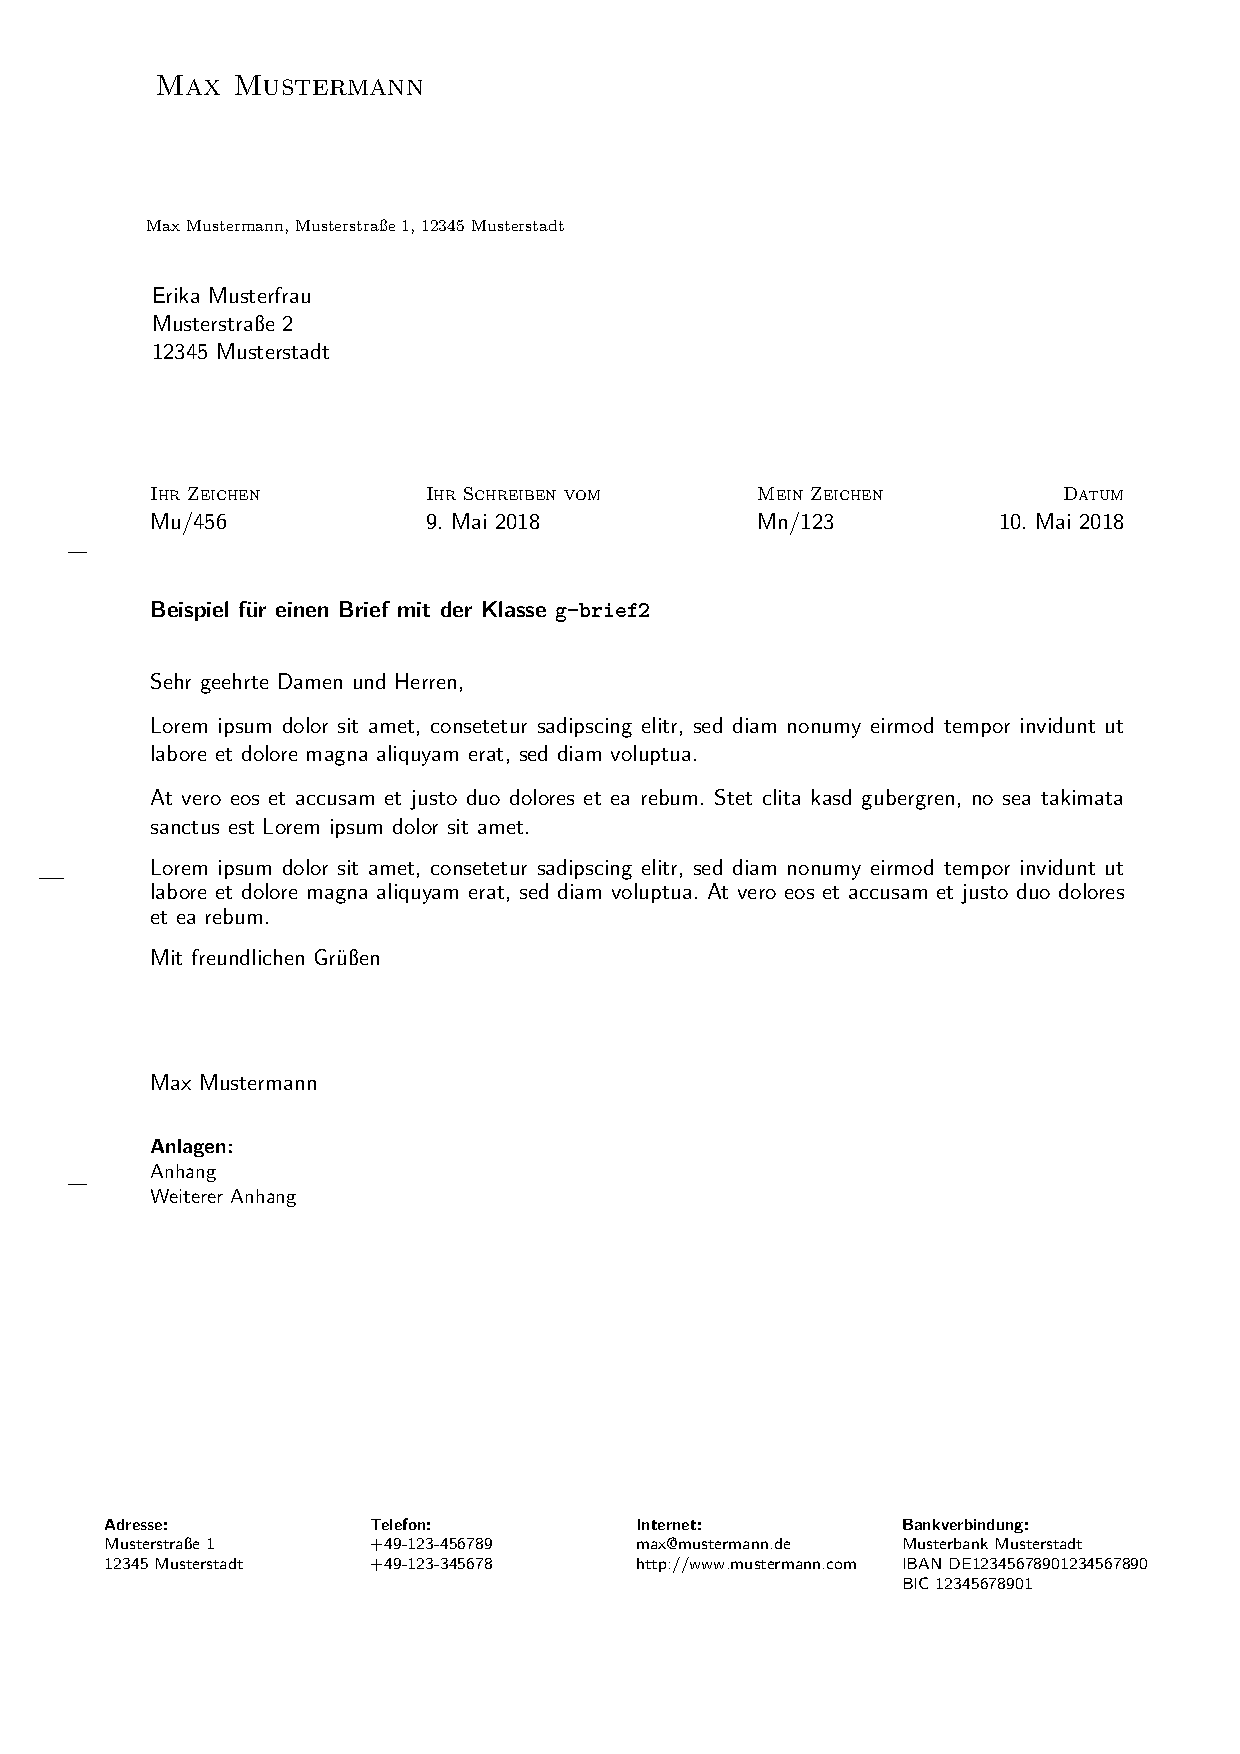
\includegraphics[page=1, width=.98\textwidth]{Beispiele/Brief_gbrief2/brief_gbrief2.pdf}}
    \caption{Resultat von Listing~\ref{beispielgbrief2}}
    \label{fig_gbrief2}
\end{figure}


\section{Briefe mit der Dokumentklasse \texttt{scrlttr2}}
\index[cmd]{\texttt{scrlttr2}}

Eine moderne Alternative zur Dokumentklasse \verb!g-brief2! ist die Klasse \verb!scrlttr2!. Diese ist Teil des \LaTeXe-Erweiterungspakets KOMA-Script. Die Klasse bietet vielfältige Optionen zur Briefgestaltung und ist auch in deutscher Sprache umfangreich dokumentiert~\cite{KOMAScript_Dokumentation}.

\lstinputlisting[caption={Ein Beispiel zur Dokumentklasse \texttt{scrlttr2}},label=beispielscrlttr2, style=customlatex]{Beispiele/Brief_scrlttr2/brief_scrlttr2.tex}


\begin{figure}[H]
%     \centering
         % Abschneiden mit trim = liks unten rechts oben
         \fbox{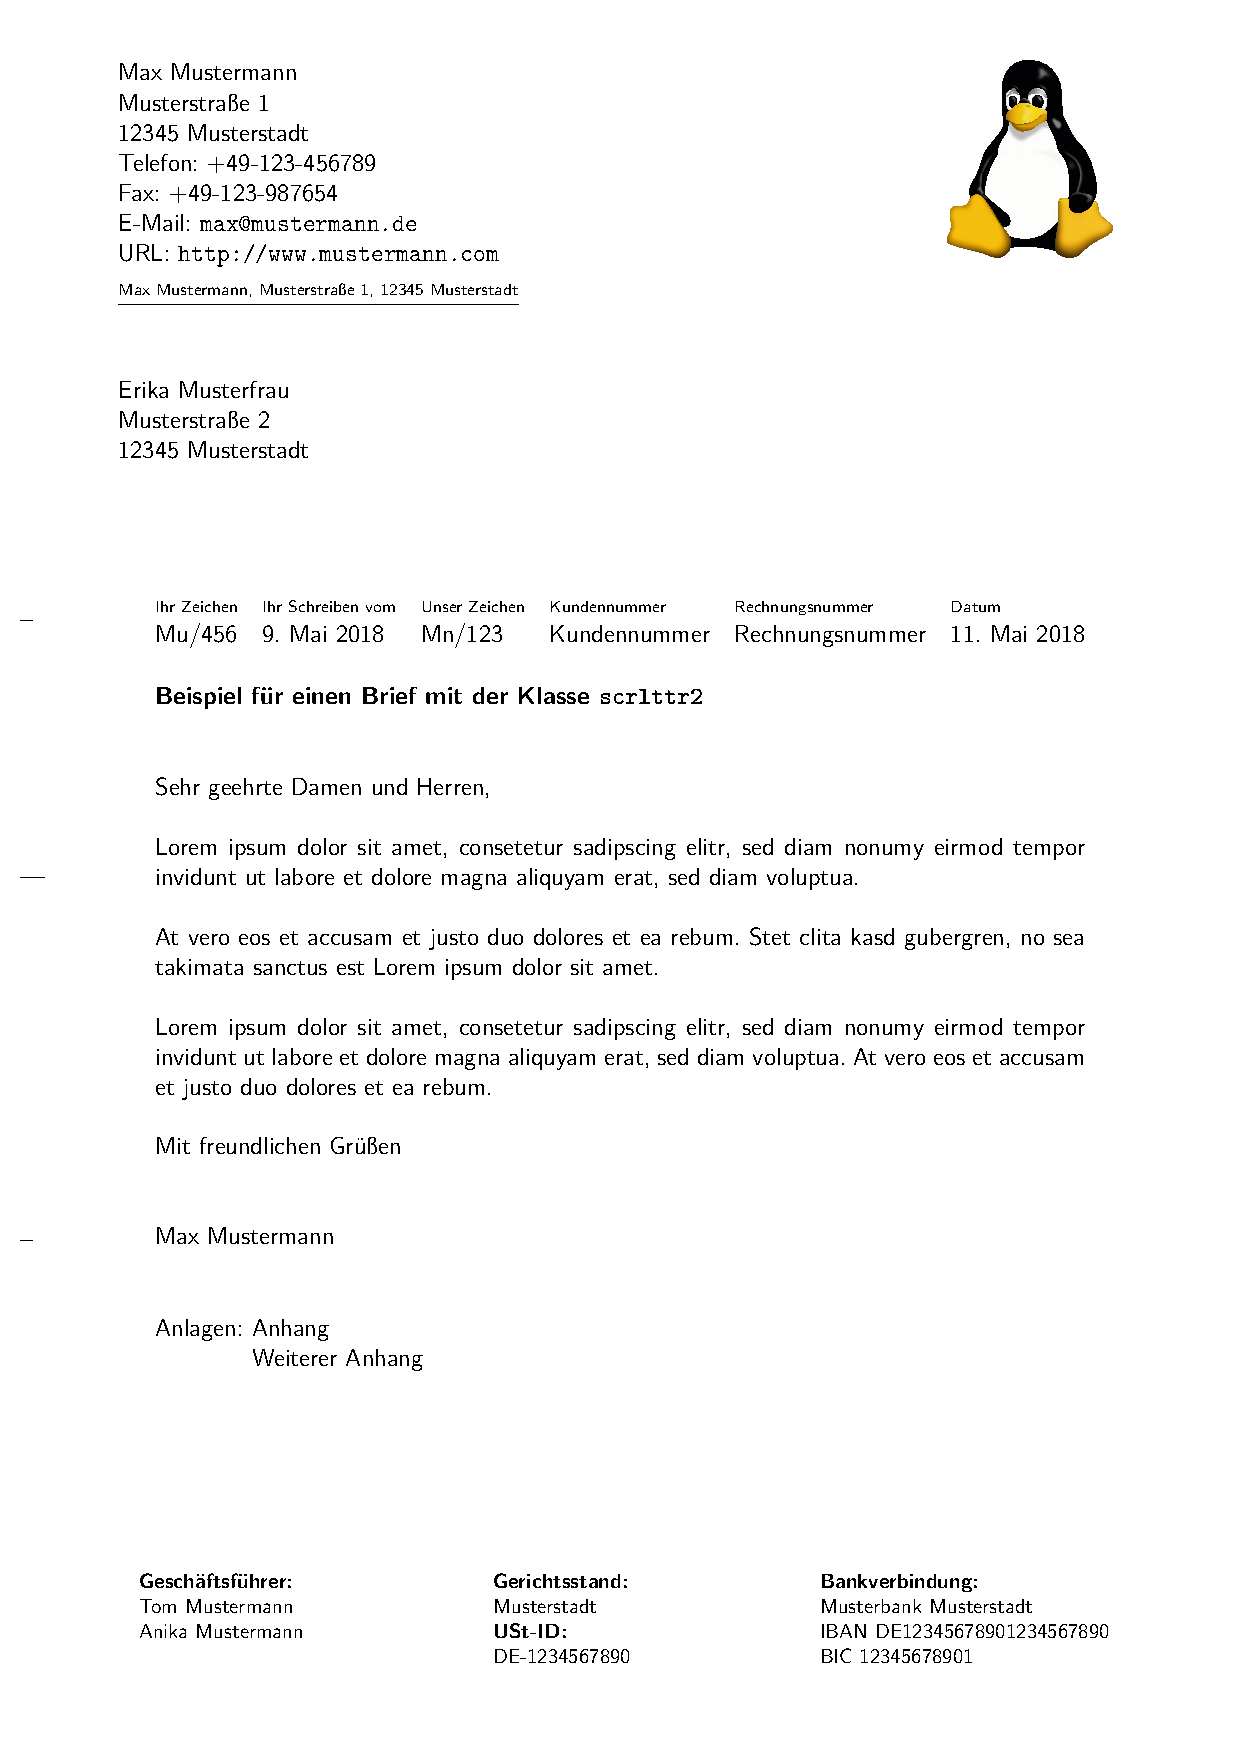
\includegraphics[page=1, width=.98\textwidth]{Beispiele/Brief_scrlttr2/brief_scrlttr2.pdf}}
    \caption{Resultat von Listing~\ref{beispielscrlttr2}}
    \label{fig_scrlttr2}
\end{figure}


\chapter{Sonderschriften}

Standardmäßig verwendet \LaTeX\ die Schrift Computer Modern. Diese verleiht 
Dokumenten einen gewissen \glqq\LaTeX-Look\grqq. 
Die Verwendung anderer Schriften, auch ungewöhnlicher Schriften, ist auf verschiedene
Art und Weise möglich.

Eine hilfreiche Übersicht über freie Schriften und Beschreibungen, wie diese in eigenen Dokumenten verwendet
werden können, bietet der \LaTeX\ Font Catalogue~\cite{LaTeXFontCatalogue}.

\section{Altdeutsche Schriften}
\index{Altdeutsche Schrift}
\index{Buchstaben!Altdeutsche}

Eine Möglichkeit, um altdeutsche Schriften zu verwenden, ist die Nutzung des 
Erweiterungspakets \verb!yfonts!~\cite{TypesettingOldGermanFonts_Dokumentation}. Nachdem es mit dem Befehl \verb!\usepackage{yfonts}! in der Präambel der Quelldatei
eingebunden ist, stehen die Befehle 
\verb!\textgoth! \index[cmd]{\texttt{\textbackslash textgoth}}
für \textgoth{Gotische Schrift}, 
\verb!\textswab! \index[cmd]{\texttt{\textbackslash textswab}}
für \textswab{Schwabacher Schrift}
und \verb!\textfrak! \index[cmd]{\texttt{\textbackslash textfrak}}
für \textfrak{Fraktur} zur Verfügung.

\begin{boxedminipage}{\textwidth}
\texttt{\textbackslash textgoth\{}\textsl{Text}\texttt{\}} \\
\texttt{\textbackslash textswab\{}\textsl{Text}\texttt{\}} \\
\texttt{\textbackslash textfrak\{}\textsl{Text}\texttt{\}}
\end{boxedminipage}

\section{Barcodes}
\index{Barcode}

Es existieren mehrere Erweiterungspakete, um Barcodes komfortabel zu setzen.
Ein Beispiel ist das Erweiterungspaket \verb!makebarcode!~\cite{Barcodes_Dokumentation}, das den Befehl \verb!\barcode!\index[cmd]{\texttt{\textbackslash barcode}} definiert.

\begin{boxedminipage}{\textwidth}
\texttt{\textbackslash barcode\{}\textsl{Text}\texttt{\}} 
\end{boxedminipage}

Der folgende Befehl in der Präambel der Quelldatei bindet das Erweiterungspaket ein und definiert die Kodierung Code 39, 
eine Zeichenhöhe (Parameter \verb!H!) von 1\,cm, das dünne Linien 0,5\,mm breit (Parameter \verb!X!) sind und das dicke Linien 2,5 mal so breit sind wie dünne Linien (Parameter \verb!ratio!).

\begin{boxedminipage}{\textwidth}
\verb!\usepackage[code=Code39,X=.5mm,ratio=2.5,H=1cm]{makebarcode}!
\end{boxedminipage}

In der Praxis sehen einzelne Zeichen dann wie in Tabelle~\ref{Tabelle_Barcodes} aus.

\begin{table}[h!tb]
\centering
\begin{longtable}{ccccc}
\caption{Einzelne Zeichen, als Barcodes gesetzt}
\label{Tabelle_Barcodes}       % Give a unique label
\endfirsthead
\endhead
0 & 1 & 2 & 3 & 4 \\ 
\barcode{0} & \barcode{1} & \barcode{2} & \barcode{3} & \barcode{4} \\
5 & 6 & 7 & 8 & 9 \\
\barcode{5} & \barcode{6} & \barcode{7} & \barcode{8} & \barcode{9} \\
+ & - & / & . & A \\
\barcode{+} & \barcode{-} & \barcode{/} & \barcode{.} & \barcode{A} \\
B & C & D & E & F \\
\barcode{B} & \barcode{C} & \barcode{D} & \barcode{E} & \barcode{F} \\
G & H & I & J & K \\
\barcode{G} & \barcode{H} & \barcode{I} & \barcode{J} & \barcode{K} \\
L & M & N & O & P \\
\barcode{L} & \barcode{M} & \barcode{N} & \barcode{O} & \barcode{P} \\
Q & R & S & T & U \\
\barcode{Q} & \barcode{R} & \barcode{S} & \barcode{T} & \barcode{U} \\
V & W & X & Y & Z \\
\barcode{V} & \barcode{W} & \barcode{X} & \barcode{Y} & \barcode{Z} \\
\end{longtable}
\end{table}


\section{QR-Codes}
\label{Abschnitt_QR-Code}
\index{QR-Code}

Bei QR-Codes\footnote{Das QR steht für Quick Response} handelt es sich um zweidimensionale Codes für Zeichenketten.
Ein QR-Code besteht aus einer quadratischen Matrix aus schwarzen und weißen Quadraten, die die kodierten Daten binär darstellen. 
Der maximale Informationsgehalt eines QR-Codes (177x177 Elemente) beträgt ca. 3\,kB).~\cite{QRCode_Wikipedia}
Mobiltelefone verfügen in der Regel über eine Software, die in der 
Lage ist, QR-Codes zu erkennen und zu dekodieren. Eine typische Anwendung ist es, Internetadressen als
QR-Codes bereitzustellen, um diese einfach und ohne manuelle Eingabe an ein mobiles Gerät zu übertragen.

Zum Erstellen von QR-Codes ist es unter anderem möglich, das Erweiterungspaket \verb!qrcode! zu nutzen.
Dieses Paket bietet zahlreiche Möglichkeiten, Informationen als QR-Codes zu kodieren, und es definiert hierzu den 
Befehl \verb!\qrcode!\index[cmd]{\texttt{\textbackslash qrcode}}.




\begin{boxedminipage}{\textwidth}
\texttt{\textbackslash qrcode\{}\textsl{Optionen}\texttt{\}\{}\textsl{Text}\texttt{\}}
\end{boxedminipage}


Von den möglichen Optionen des Befehls ist an dieser Stelle nur \verb!height! vorgestellt. Hier ist die Höhe (und Breite) des zu 
erzeugenden QR-Codes inklusive einer Maßeinheit 
(siehe Abschnitt~\ref{sec:Massangaben}) definiert. Um beispielsweise einen QR-Code mit der URL zu diesem Werk zu erzeugen, der 3\,cm hoch und breit ist, 
genügt der folgende Befehl: 

\begin{lstlisting}[label=QRcode, style=customlatex]
\qrcode[height=3cm]{https://github.com/christianbaun/einstieginlatex}
\end{lstlisting}

Das Ergebnis sieht wie folgt aus:

\qrcode[height=3cm]{https://github.com/christianbaun/einstieginlatex}

\section{Besondere Zeichen}

Ein Zeichensatz, der statt Buchstaben, 
Ziffern und Satzzeichen mit 
Sonderzeichen aller Art gefüllt ist, ist \textsl{ZapfDingbats}\index{ZapfDingbats} (siehe Tabelle~\ref{Tabelle_Font_ZapfDingbats}).
Dessen Verwendung ist mit dem Erweiterungspaket \verb!pifont.sty! 
besonders einfach. 

\begin{longtable}{c|p{.9cm}|p{.9cm}|p{.9cm}|p{.9cm}|p{.9cm}|p{.9cm}|p{.9cm}|p{.9cm}}
\caption{Zeichen aus dem Font ZapfDingbats}
\label{Tabelle_Font_ZapfDingbats}       % Give a unique label
\endfirsthead
\endhead
& \multicolumn{1}{c|}{\textquotesingle 0} & \multicolumn{1}{c|}{\textquotesingle 1} & \multicolumn{1}{c|}{\textquotesingle 2} 
& \multicolumn{1}{c|}{\textquotesingle 3} & \multicolumn{1}{c|}{\textquotesingle 4} & \multicolumn{1}{c|}{\textquotesingle 5}
& \multicolumn{1}{c|}{\textquotesingle 6} & \multicolumn{1}{c}{\textquotesingle 7} \\
\hline
\textquotesingle 04x & & 
{\ding{33}}\hfill\tiny{33} & 
{\ding{34}}\hfill\tiny{34} & 
{\ding{35}}\hfill\tiny{35} & 
{\ding{36}}\hfill\tiny{36} & 
{\ding{37}}\hfill\tiny{37} & 
{\ding{38}}\hfill\tiny{38} & 
{\ding{39}}\hfill\tiny{39}  \\
\hline
\textquotesingle 05x & 
{\ding{40}}\hfill\tiny{40} & 
{\ding{41}}\hfill\tiny{41} & 
{\ding{42}}\hfill\tiny{42} & 
{\ding{43}}\hfill\tiny{43} & 
{\ding{44}}\hfill\tiny{44} & 
{\ding{45}}\hfill\tiny{45} & 
{\ding{46}}\hfill\tiny{46} & 
{\ding{47}}\hfill\tiny{47}  \\ 
\hline
\textquotesingle 06x & 
{\ding{48}}\hfill\tiny{48} & 
{\ding{49}}\hfill\tiny{49} & 
{\ding{50}}\hfill\tiny{50} & 
{\ding{51}}\hfill\tiny{51} & 
{\ding{52}}\hfill\tiny{52} & 
{\ding{53}}\hfill\tiny{53} & 
{\ding{54}}\hfill\tiny{54} & 
{\ding{55}}\hfill\tiny{55}  \\
\hline
\textquotesingle 07x & 
{\ding{56}}\hfill\tiny{56} & 
{\ding{57}}\hfill\tiny{57} & 
{\ding{58}}\hfill\tiny{58} & 
{\ding{59}}\hfill\tiny{59} & 
{\ding{60}}\hfill\tiny{60} & 
{\ding{61}}\hfill\tiny{61} & 
{\ding{62}}\hfill\tiny{62} & 
{\ding{63}}\hfill\tiny{63}  \\
\hline
\textquotesingle 10x &
{\ding{64}}\hfill\tiny{64} & 
{\ding{65}}\hfill\tiny{65} & 
{\ding{66}}\hfill\tiny{66} & 
{\ding{67}}\hfill\tiny{67} & 
{\ding{68}}\hfill\tiny{68} & 
{\ding{69}}\hfill\tiny{69} & 
{\ding{70}}\hfill\tiny{70} & 
{\ding{71}}\hfill\tiny{71} \\
\hline
\textquotesingle 11x & 
{\ding{72}}\hfill\tiny{72} & 
{\ding{73}}\hfill\tiny{73} & 
{\ding{74}}\hfill\tiny{74} & 
{\ding{75}}\hfill\tiny{75} & 
{\ding{76}}\hfill\tiny{76} & 
{\ding{77}}\hfill\tiny{77} & 
{\ding{78}}\hfill\tiny{78} & 
{\ding{79}}\hfill\tiny{79}  \\
\hline
\textquotesingle 12x & 
{\ding{80}}\hfill\tiny{80} & 
{\ding{81}}\hfill\tiny{81} & 
{\ding{82}}\hfill\tiny{82} & 
{\ding{83}}\hfill\tiny{83} & 
{\ding{84}}\hfill\tiny{84} & 
{\ding{85}}\hfill\tiny{85} & 
{\ding{86}}\hfill\tiny{86} & 
{\ding{87}}\hfill\tiny{87}  \\
\hline
\textquotesingle 13x &
{\ding{88}}\hfill\tiny{88} & 
{\ding{89}}\hfill\tiny{89} & 
{\ding{90}}\hfill\tiny{90} & 
{\ding{91}}\hfill\tiny{91} & 
{\ding{92}}\hfill\tiny{92} & 
{\ding{93}}\hfill\tiny{93} & 
{\ding{94}}\hfill\tiny{94} & 
{\ding{95}}\hfill\tiny{95} \\
\hline
\textquotesingle 14x & 
{\ding{96}}\hfill\tiny{96} & 
{\ding{97}}\hfill\tiny{97} & 
{\ding{98}}\hfill\tiny{98} & 
{\ding{99}}\hfill\tiny{99} & 
{\ding{100}}\hfill\tiny{100} & 
{\ding{101}}\hfill\tiny{101} & 
{\ding{102}}\hfill\tiny{102} & 
{\ding{103}}\hfill\tiny{103}  \\
\hline
\textquotesingle 15x & 
{\ding{104}}\hfill\tiny{104} & 
{\ding{105}}\hfill\tiny{105} & 
{\ding{106}}\hfill\tiny{106} & 
{\ding{107}}\hfill\tiny{107} & 
{\ding{108}}\hfill\tiny{108} & 
{\ding{109}}\hfill\tiny{109} & 
{\ding{110}}\hfill\tiny{110} & 
{\ding{111}}\hfill\tiny{111}  \\
\hline
\textquotesingle 16x & 
{\ding{112}}\hfill\tiny{112} & 
{\ding{113}}\hfill\tiny{113} & 
{\ding{114}}\hfill\tiny{114} & 
{\ding{115}}\hfill\tiny{115} & 
{\ding{116}}\hfill\tiny{116} & 
{\ding{117}}\hfill\tiny{117} & 
{\ding{118}}\hfill\tiny{118} & 
{\ding{119}}\hfill\tiny{119}  \\
\hline
\textquotesingle 17x & 
{\ding{120}}\hfill\tiny{120} & 
{\ding{121}}\hfill\tiny{121} & 
{\ding{122}}\hfill\tiny{122} & 
{\ding{123}}\hfill\tiny{123} & 
{\ding{124}}\hfill\tiny{124} & 
{\ding{125}}\hfill\tiny{125} & 
{\ding{126}}\hfill\tiny{126} &  \\
\hline
\textquotesingle 26x & & 
{\ding{161}}\hfill\tiny{161} & 
{\ding{162}}\hfill\tiny{162} & 
{\ding{163}}\hfill\tiny{163} & 
{\ding{164}}\hfill\tiny{164} & 
{\ding{165}}\hfill\tiny{165} & 
{\ding{166}}\hfill\tiny{166} & 
{\ding{167}}\hfill\tiny{167}  \\
\hline
\textquotesingle 27x & 
{\ding{168}}\hfill\tiny{168} & 
{\ding{169}}\hfill\tiny{169} & 
{\ding{170}}\hfill\tiny{170} & 
{\ding{171}}\hfill\tiny{171} & 
{\ding{172}}\hfill\tiny{172} & 
{\ding{173}}\hfill\tiny{173} & 
{\ding{174}}\hfill\tiny{174} & 
{\ding{175}}\hfill\tiny{175} \\
\hline
\textquotesingle 28x & 
{\ding{176}}\hfill\tiny{176} & 
{\ding{177}}\hfill\tiny{177} & 
{\ding{178}}\hfill\tiny{178} & 
{\ding{179}}\hfill\tiny{179} & 
{\ding{180}}\hfill\tiny{180} & 
{\ding{181}}\hfill\tiny{181} & 
{\ding{182}}\hfill\tiny{182} & 
{\ding{183}}\hfill\tiny{183} \\
\hline
\textquotesingle 29x & 
{\ding{184}}\hfill\tiny{184} & 
{\ding{185}}\hfill\tiny{185} & 
{\ding{186}}\hfill\tiny{186} & 
{\ding{187}}\hfill\tiny{187} & 
{\ding{188}}\hfill\tiny{188} & 
{\ding{189}}\hfill\tiny{189} & 
{\ding{190}}\hfill\tiny{190} & 
{\ding{191}}\hfill\tiny{191} \\
\hline
\textquotesingle 30x & 
{\ding{192}}\hfill\tiny{192} & 
{\ding{193}}\hfill\tiny{193} & 
{\ding{194}}\hfill\tiny{194} & 
{\ding{195}}\hfill\tiny{195} & 
{\ding{196}}\hfill\tiny{196} & 
{\ding{197}}\hfill\tiny{197} & 
{\ding{198}}\hfill\tiny{198} & 
{\ding{199}}\hfill\tiny{199}  \\
\hline
\textquotesingle 31x & 
{\ding{200}}\hfill\tiny{200} & 
{\ding{201}}\hfill\tiny{201} & 
{\ding{202}}\hfill\tiny{202} & 
{\ding{203}}\hfill\tiny{203} & 
{\ding{204}}\hfill\tiny{204} & 
{\ding{205}}\hfill\tiny{205} & 
{\ding{206}}\hfill\tiny{206} & 
{\ding{207}}\hfill\tiny{207}  \\
\hline
\textquotesingle 32x & 
{\ding{208}}\hfill\tiny{208} & 
{\ding{209}}\hfill\tiny{209} & 
{\ding{210}}\hfill\tiny{210} & 
{\ding{211}}\hfill\tiny{211} & 
{\ding{212}}\hfill\tiny{212} & 
{\ding{213}}\hfill\tiny{213} & 
{\ding{214}}\hfill\tiny{214} & 
{\ding{215}}\hfill\tiny{215}  \\
\hline
\textquotesingle 33x & 
{\ding{216}}\hfill\tiny{216} & 
{\ding{217}}\hfill\tiny{217} & 
{\ding{218}}\hfill\tiny{218} & 
{\ding{219}}\hfill\tiny{219} & 
{\ding{220}}\hfill\tiny{220} & 
{\ding{221}}\hfill\tiny{221} & 
{\ding{222}}\hfill\tiny{222} & 
{\ding{223}}\hfill\tiny{223}  \\
\hline
\textquotesingle 34x & 
{\ding{224}}\hfill\tiny{224} & 
{\ding{225}}\hfill\tiny{225} & 
{\ding{226}}\hfill\tiny{226} & 
{\ding{227}}\hfill\tiny{227} & 
{\ding{228}}\hfill\tiny{228} &
{\ding{229}}\hfill\tiny{229} &
{\ding{230}}\hfill\tiny{230} &
{\ding{231}}\hfill\tiny{231}  \\
\hline
\textquotesingle 35x & 
{\ding{232}}\hfill\tiny{232} & 
{\ding{233}}\hfill\tiny{233} & 
{\ding{234}}\hfill\tiny{234} & 
{\ding{235}}\hfill\tiny{235} & 
{\ding{236}}\hfill\tiny{236} &
{\ding{237}}\hfill\tiny{237} &
{\ding{238}}\hfill\tiny{238} &
{\ding{239}}\hfill\tiny{239}  \\
\hline
\textquotesingle 36x & & 
{\ding{241}}\hfill\tiny{241} & 
{\ding{242}}\hfill\tiny{242} & 
{\ding{243}}\hfill\tiny{243} & 
{\ding{244}}\hfill\tiny{244} &
{\ding{245}}\hfill\tiny{245} &
{\ding{246}}\hfill\tiny{246} &
{\ding{247}}\hfill\tiny{247}  \\
\hline
\textquotesingle 37x & 
{\ding{248}}\hfill\tiny{248} & 
{\ding{249}}\hfill\tiny{249} & 
{\ding{250}}\hfill\tiny{250} & 
{\ding{251}}\hfill\tiny{251} & 
{\ding{252}}\hfill\tiny{252} &
{\ding{253}}\hfill\tiny{253} &
{\ding{254}}\hfill\tiny{254} &  \\
\end{longtable}

Das Einbinden des Erweiterungspakets in eigene Dokumente 
geschieht mit dem Befehl \verb!\usepackage{pifont}! in der 
Präambel des Dokuments.

Ein Befehl, den das Erweiterungspaket definiert, ist \verb!\ding!\index[cmd]{\texttt{ding}}, um einzelne Zeichen aus dem Font
\textsl{ZapfDingbats} auszugeben.

\begin{boxedminipage}{\textwidth}
\texttt{\textbackslash ding\{}\textsl{Zeichen}\texttt{\}} 
\end{boxedminipage}

Dem Befehl wird die Nummer (siehe Tabelle~\ref{Tabelle_Font_ZapfDingbats}) des Zeichens, das gesetzt werden soll, in geschweiften Klammern als Argument übergeben. Die Schneeflocke 
\ding{100} mit der Zeichennummer \verb!100! beispielsweise setzt der Befehl 
\verb!\ding{100}!. 

Alternativ kann auf die einzelnen Zeichen auch durch die Angabe der Kombination aus Zeilen- und Spaltennummer angeben werden. Die In diesem Fall wird ein einzelnes Anführungszeichen der Zeichennummer vorgestellt. Die bereits beschriebene Schneeflocke befindet sich in Zeile 14 und Spalte 4. Das heißt, sie kann auch mit diesem Befehl gesetzt werden: \verb!\ding{'144}!

Zwei weitere Befehle, die das Erweiterungspaket \verb!pifont! definiert,
sind \verb!\dingline! und \verb!\dingfill!.

\begin{boxedminipage}{\textwidth}
\texttt{\textbackslash dingline\{}\textsl{Zeichen}\texttt{\}} \\
\texttt{\textbackslash dingfill\{}\textsl{Zeichen}\texttt{\}} 
\end{boxedminipage}

Wird der Befehl \verb!\dingline!\index[cmd]{\texttt{dingline}} ausgeführt, beginnt der \LaTeX-Compiler eine neue Zeile, die mit dem als Argument übergeben  
Zeichen gefüllt wird. Die beidseitige Einrückung
entspricht 0,5\,Zoll (also ca. 1,3\,cm). Ein sinnvolles Anwendungsbeispiel für diesen Befehl sind Formulare, wo ein Teil des Blattes 
abgetrennt werden soll, beispielsweise so: 

\dingline{34}

Die Zeile mit den Scheren erzeugt der Befehl \verb!\dingline{34}!.

Im Gegensatz zu \verb!\dingline! wird bei \verb!\dingfill!\index[cmd]{\texttt{dingfill}} nur der 
in einer Zeile verfügbare Leerraum mit dem als Argument übergeben  
Zeichen gefüllt. So erzeugt der Befehl \verb!\dingfill{51}! hier: \dingfill{51}

Der Befehl \verb!\dingfill! füllt immer bis zum Zeilenende.
Es sei denn, es folgt noch ein Text nach dem Befehl. 
Der Befehl \verb!\dingfill{51}! gefolgt von der Zeichenkette \verb!Ende.! erzeugt folgendes Ergebnis: \dingfill{51} Ende. 

Außer den bereits vorgestellten Befehlen definiert das Erweiterungspaket \verb!pifont! auch die Umgebung
\verb!dinglist!\index[cmd]{\texttt{dinglist}}. Diese ermöglicht es Aufzählungen (siehe Abschnitt~\ref{Abschnitt_Aufzaehlungen})
ähnlich wie \verb!itemize! zu setzen.

\begin{boxedminipage}{\textwidth}
\texttt{\textbackslash begin\{dinglist\}\{}\textsl{Zeichen}\texttt{\}}  \enskip \dots\ \enskip \texttt{\textbackslash end\{dinglist\}} 
\end{boxedminipage}

Die einzelnen Listenpunkte beginnen wie gehabt mit dem Befehl \verb!\item!.

Bei der Umgebung \verb!dinglist! wird die Nummer (siehe Tabelle~\ref{Tabelle_Font_ZapfDingbats}) des Zeichens, das als Markierungszeichen für jeden Auflistungspunkt verwendet werden soll, in geschweiften Klammern als Argument übergeben.

\begin{minipage}[h]{0.5\textwidth}
\setlength{\parskip}{1em}
\frenchspacing
\begin{Verbatim}[frame=single]
\begin{dinglist}{52}
  \item Erster Listenpunkt
  \item Zweiter Listenpunkt
  \begin{dinglist}{234}
    \item Erster Unterpunkt
    \item Zweiter Unterpunkt
  \end{dinglist}
  \item Dritter Listenpunkt
\end{dinglist}
\end{Verbatim}
\end{minipage}
\hfill
\begin{minipage}[h]{0.48\textwidth}
\setlength{\parskip}{1em}
\frenchspacing
\begin{dinglist}{52}
  \item Erster Listenpunkt
  \item Zweiter Listenpunkt
  \begin{dinglist}{234}
    \item Erster Unterpunkt
    \item Zweiter Unterpunkt
  \end{dinglist}
  \item Dritter Listenpunkt
\end{dinglist}
\end{minipage}

Neben der Umgebung \verb!dinglist!, die ein Äquivalent zur Umgebung \verb!itemize! ist, definiert
das Erweiterungspaket \verb!pifont! mit der Umgebung \verb!dingautolist! auch ein Äquivalent zur 
Umgebung \verb!enumerate!.

\begin{boxedminipage}{\textwidth}
\texttt{\textbackslash begin\{dingautolist\}\{}\textsl{Zeichen}\texttt{\}}  \enskip \dots\ \enskip \texttt{\textbackslash end\{dingautolist\}} 
\end{boxedminipage}

Im Gegensatz zur \verb!dinglist! wird bei der Umgebung \verb!dingautolist!\index[cmd]{\texttt{dingautolist}}
mit jedem weiteren Aufzählungspunkt 
(\verb!\item!) die Nummer des verwendeten Zeichens um eins erhöht. 
Konkret wird in der Zeichentabelle (siehe Tabelle~\ref{Tabelle_Font_ZapfDingbats}) 
immer ein Zeichen weiter gegangen. So hat jeder Aufzählungspunkt einer Ebene ein anderes
Markierungszeichen.


% \begin{figure}[H]
\begin{minipage}[h]{0.5\textwidth}
\setlength{\parskip}{1em}
\frenchspacing
\begin{Verbatim}[frame=single]
\begin{dingautolist}{172}
  \item Erster Aufzählungspunkt
  \item Zweiter Aufzählungspunkt
  \begin{dingautolist}{182}
    \item Erster Unterpunkt
    \item Zweiter Unterpunkt
  \end{dingautolist}
  \item Dritter Aufzählungspunkt
\end{dingautolist}
\end{Verbatim}
\end{minipage}
\hfill
\begin{minipage}[h]{0.48\textwidth}
\setlength{\parskip}{1em}
\frenchspacing
\begin{dingautolist}{172}
  \item Erster Aufzählungspunkt
  \item Zweiter Aufzählungspunkt
  \begin{dingautolist}{182}
    \item Erster Unterpunkt
    \item Zweiter Unterpunkt
  \end{dingautolist}
  \item Dritter Aufzählungspunkt
\end{dingautolist}
\end{minipage}
% \end{figure}


\section{Kalligrafie}

Das Erweiterungspaket \verb!calligra!~\cite{Calligra_Dokumentation} bietet definiert den Befehl 
\verb!\textcalligra!\index[cmd]{\texttt{\textbackslash textcalligra}}
und bietet dadurch eine einfache Möglichkeit, Texte in einem 
Kalligrafie-Font zu setzen.

\begin{boxedminipage}{\textwidth}
\texttt{\textbackslash textcalligra\{}\textsl{Text}\texttt{\}}
\end{boxedminipage}

\begin{minipage}[h]{0.54\textwidth}
\setlength{\parskip}{1em}
\frenchspacing
\begin{Verbatim}[frame=single]
\textcalligra{Lorem ipsum dolor sit 
amet, consetetur sadipscing elitr, 
sed diam nonumy eirmod tempor 
invidunt ut labore et dolore magna 
aliquyam erat, sed diam voluptua. 
At vero eos et accusam et justo duo 
dolores et ea rebum.}

\textcalligra{0123456789}
\end{Verbatim}
\end{minipage}
\hfill
\begin{minipage}[h]{0.38\textwidth}
\setlength{\parskip}{1em}
\frenchspacing
\textcalligra{Lorem ipsum dolor sit amet, consetetur sadipscing elitr, sed diam nonumy eirmod tempor invidunt ut labore et dolore magna aliquyam erat, sed diam voluptua. At vero eos et accusam et justo duo dolores et ea rebum.}

\textcalligra{0123456789}
\end{minipage}


\chapter{Literaturverzeichnis}
\label{Kapitel_Literaturverzeichnis}
\index{Literaturverzeichnis}

Das Einbinden eines Literaturverzeichnisses in Dokumente kann auf verschiedene Arten geschehen. Unterschiede in den Vorgehensweisen bestehen in erster Linie hinsichtlich des Automatisierungsgrads. In diesem Dokument ist das Erstellen von Literaturverzeichnissen mit der Umgebung \verb!thebibliography! und mit Bib\TeX\ beschrieben.

Ganz unabhängig von der Art und Weise, wie das Literaturverzeichnis realisiert wird, geschieht der Verweis auf Einträge im Literaturverzeichnis mit dem Befehl \verb|\cite|.\index[cmd]{\texttt{\textbackslash cite}}

\begin{boxedminipage}{\textwidth}
	\texttt{\textbackslash cite[\textsl{Text}]\{\textsl{Schlüssel}\}} 
\end{boxedminipage}

Der zwingend nötige Parameter \textsl{Schlüssel} verweist auf einen oder mehrere Einträge im Literaturverzeichnis. Der Inhalt des optionalen Parameters  \textsl{Text} wird zusätzlich ausgegeben und kann eine weiterführende Information für den Leser enthalten wie zum Beispiel \glqq S.\,42-46\grqq\ oder \glqq Kapitel 5\grqq.

Soll auf mehrere Einträge im Literaturverzeichnis gleichzeitig referenziert werden, müssen die Angaben im Parameter \textsl{Schlüssel} durch Kommata voneinander getrennt sein.

\section{Manueller Satz des Literaturverzeichnisses}
\label{Abschnitt_thebibliography}

Das Einfügen des des Literaturverzeichnisses in das Dokument geschieht mit einer Umgebung \verb!thebibliography! am Ende des \LaTeX-Quelltextes.
\index[cmd]{\texttt{thebibliography}}

\begin{boxedminipage}{\textwidth}
	\texttt{\textbackslash begin\{thebibliography\}\{\textsl{Markierungsbreite}\}} \enskip \dots\ \enskip \texttt{\textbackslash end\{thebibliography\}} 
\end{boxedminipage}

Die Breite (Anzahl der Zeichen) der einzelnen Labels (Markierungen) im Literaturverzeichniss definiert der Inhalt des Parameters \textsl{Markierungsbreite}. Dieser kann eine beliebige Zeichenkette enthalten (z.B. \verb|999|)~\cite{voss2007referenz}.

Die einzelnen Einträge im Literaturverzeichnis realisiert der Befehl \verb|\bibitem| innerhalb der Umgebung \verb!thebibliography!. 
\index[cmd]{\texttt{\textbackslash bibitem}}

\begin{boxedminipage}{\textwidth}
	\texttt{\textbackslash bibitem[\textsl{Markierung}]\{\textsl{Schlüssel}\} \textsl{Text}} 
\end{boxedminipage}

Ein Beispiel für eine \verb!thebibliography!-Umgebung mit drei Einträgen enthält Listing~\ref{listing_thebibliography_beispiel}. Das resultierende Literaturverzeichnis zeigt Abbildung~\ref{fig_thebibliography_beispiel}.

\begin{lstlisting}[caption={Ein Literaturverzeichnis mit der Umgebung \texttt{thebibliography}},label=listing_thebibliography_beispiel, style=customlatex]
\begin{thebibliography}{9}
\bibitem[Go93]{GoMiSa93} 
Michel Goossens, Frank Mittelbach and Alexander Samarin. 
\emph{The \LaTeX\ Companion}. 
Addison-Wesley, Reading, Massachusetts, 1993.
\bibitem[La94]{Lamport94}
Leslie Lamport,	\emph{\LaTeX: A Document Preparation System},	
Addison Wesley, Massachusetts, 2nd edition, 1994.
\bibitem[Kn86]{Knuth96} 
Donald E. Knuth, \emph{Computers and Typesetting -- Volume A: 
The \TeX book}, Addison Wesley, 1986.
\end{thebibliography}
\end{lstlisting}

\begin{figure}[H]
	%     \centering
	% Abschneiden mit trim = liks unten rechts oben
	\fbox{\includegraphics[page=1, clip, trim=2cm 22cm 2cm 2cm, width=.98\textwidth]{Beispiele/thebibliography/thebibliography_beispiel.pdf}}
	\caption{Resultat von Listing~\ref{listing_thebibliography_beispiel}}
	\label{fig_thebibliography_beispiel}
\end{figure}

Ein Unterschied zum Satz des Literaturverzeichnisses mit Bib\TeX\ ist, das es für das Aussehen und den Umfang des Literaturverzeichnisses keine Rolle spielt, ob im Dokument auf einzelne Einträge referenziert wird. 
Das Literaturverzeichnis im fertig gesetzten Dokument enthält immer alle im Quelltext aufgeführten Einträge.

\section{Autmoatisierter Satz des Literaturverzeichnisses}
\label{Abschnitt_bibtex}
\index{Bib\TeX}

Vielfältige Möglichkeiten ein Literaturverzeichniss einzufügen und dessen Formatierung zu beeinflussen bietet \LaTeX\ in Zusammenarbeit mit dem Programm Bib\TeX\ und den Befehlen \verb|\bibliography| und \verb|\bibliographystyle|. Die Kombination aus diesen Programmen und Befehlen ermöglicht es, Quellen aus einer oder mehreren Literaturdatenbanken herauszusuchen und beispielsweise nach dem Nachnamen des ersten Autors oder gemäß der Reihenfolge der Referenzierung im Dokument zu sortieren. 

Die Einbindung einer Literaturdatenbank (\verb|.bib|-Datei) geschieht mit dem Befehl \verb|\bibliography|\index[cmd]{\texttt{\textbackslash bibliography}}. Der Dateiname wird ohne Dateiendung angegeben.

\begin{boxedminipage}{\textwidth}
	\texttt{\textbackslash bibliography\{\textsl{Dateiname}\}} 
\end{boxedminipage}

Sollen mehrere Literaturdatenbanken eingebunden werden, müssen die entsprechenden \verb|.bib|-Dateien durch Kommata voneinander abgetrennt sein. Auch hierbei werden die Dateinamen ohne Dateiendung angegeben.

\begin{boxedminipage}{\textwidth}
	\texttt{\textbackslash bibliography\{\textsl{Dateiname1},\textsl{Dateiname2},\textsl{Dateiname3},...\}} 
\end{boxedminipage}

Die Definition des Stils des Literaturverzeichnisses geschieht mit dem Befehl \verb|\bibliographystyle|\index[cmd]{\texttt{\textbackslash bibliographystyle}}.

\begin{boxedminipage}{\textwidth}
	\texttt{\textbackslash bibliographystyle\{\textsl{Stil}\}} 
\end{boxedminipage}

Der Befehl darf an (fast) beliebiger Stelle in der \verb!.tex!-Quelldatei stehen.

Es existiert eine sehr große Anzahl an Stilen. Umfangreiche Übersichten enthalten unter anderem~\cite{voss2007referenz} und~\cite{BibtexStylesShareLaTeXWebseite}. Eine Auswahl an häufig verwendeten Stilen enthält Tabelle~\ref{Tabelle_Stile_Literaturverzeichnisse}. 

\begin{table}[h!tb]
	\centering
	\caption[Auswahl an Stilen für Literaturverzeichnisse]{Auswahl an Stilen für Literaturverzeichnisse~\cite{Wikibooks_LaTeX_Woerterbuch}}
	\label{Tabelle_Stile_Literaturverzeichnisse}       % Give a unique label
	\begin{tabularx}{\textwidth}{lp{3cm}p{7.5cm}}
		\hline
		Stilname & Sortierung & Referenzierung  \\
		\hline
		\texttt{abbrv} & Erstautor & [IdNr] (Vornamen nur als Initialen) \\
		\texttt{alpha} & Erstautor & bis zu drei Anfangsbuchstaben der Autorennamen, evtl. ein hochgestelltes Pluszeichen, bei mehr als drei Autoren, Jahresangabe zweistellig \\			
		\texttt{apalike} & Erstautor & [Autorenname(n), Jahr] \\
		\texttt{plain}   & Erstautor & [IdNr] (Vornamen werden ausgeschrieben) \\
        \texttt{plainyr} & Referenzart, Jahr   & [IdNr] (Vornamen werden ausgeschrieben) \\
        \texttt{unsrt}   & Reihenfolge der Referenzierung & [IdNr] \\
		\hline
	\end{tabularx}
\end{table}

Für jeden Stil muss eine Datei gleichen Namens mit der Dateiendung \verb!.bst! existieren. Dort ist das Layout des Stils definiert.
Bei der \LaTeX-Distribution \TeX~Live befinden sich die \verb!.bst!-Dateien im Unterverzeichnis \verb|texlive/texmf-dist/bibtex/bst/|.


Bei der Arbeit mit Bib\TeX\ müssen die einzelnen Literatureinträge in einer oder mehreren Dateien mit der Dateiendung
\verb|.bib| vorliegen. Je nach Art des jeweiligen Eintrags (zum Beispiel Bücher, Artikel, technische Dokumentationen, etc.) sind bestimmte Angaben (\glqq Felder\grqq) zum Eintrag zwingend nötig oder optional möglich. Häufig verwendete Typen von Einträgen in Literaturdatenbanken sind \texttt{article}, \texttt{book}, \texttt{booklet}, \texttt{conference}, \texttt{inbook}, \texttt{incollection}, \texttt{inproceedings}, \texttt{manual}, \texttt{mastersthesis}, \texttt{misc}, \texttt{phdthesis}, \texttt{proceedings}, \texttt{techreport} und \texttt{unpublished}.

Jedem Eintrag ist ein Klammeraffe\index{Klammeraffe} (\verb!@!) vorangestellt. Es ist egal, ob das Schlüsselwort eines
Eintrags mit Klein- oder Großbuchstaben 
geschrieben ist. Jede der folgenden Schreibweisen ist somit korrekt: \verb!@book!, \verb!@BOOK!, 
\verb!@bOOk!, \verb!@BoOk!, etc.

Auf den Typ eines Eintrags folgt immer ein Paar 
geschweifter Klammern, und dazwischen befinden sich ein Schlüsselwort\index{Schlüsselwort} und 
die einzelnen Felder.
Das Schlüsselwort kann aus einer fast beliebigen
Folge von Buchstaben, 
Zahlen und Zeichen jeder Art bestehen. 
Kommata sind im Schlüsselwort tabu. 
Idealerweise ist das Schlüsselwort nicht nur eindeutig, sondern beim Lesen des Quelltextes auch nachvollziehbar.

Die einzelnen Felder bestehen 
aus jeweils einem Feldnamen
und einer Information (Feldtext).
Mögliche Felder sind u.a. \texttt{address}, \texttt{author}, \texttt{booktitle}, \texttt{chapter}, \texttt{edition}, \texttt{editor}, \texttt{isbn}, \texttt{journal}, \texttt{volume}, \texttt{month}, \texttt{note}, \texttt{number}, \texttt{organization}, \texttt{pages}, \texttt{series}, \texttt{school}, \texttt{title} und \texttt{year}. Es werden allerdings nicht alle Felder bei allen Arten von Einträgen berücksichtigt und bei allen Arten von Einträgen sind bestimmten Felder zwingend erforderlich. Eine Übrsicht über diese Typen von Einträgen in Literaturdatenbanken und deren zwingende sowie optionale Felder enthält Abschnitt~\ref{Abschnitt_Eintraege_Bibtex_Felder}.

Zwischen Feldname und Feldtext befindet sich ein \verb!=!. Der Feldtext ist von geschweiften Klammern oder alternativ mit Anführungsstrichen (\verb!" ... "!) umschlossen. Besteht der Feldtext nur aus Ziffern, sind die geschweiften Klammern bzw. Anführungsstriche unnötig.
Die einzelnen Felder sind durch Kommata voneinander getrennt.

Syntaktisch korrekt sehen Einträge in Literaturdatenbanken folgendermaßen aus: 

\begin{boxedminipage}{\textwidth}
\verb!@!\textsl{Typ}\verb!{!\textsl{Schlüsselwort}\verb!,!\newline
\verb!    !\textsl{Feldname}\verb! = {!\textsl{Feldtext}\verb!},! \newline
\verb!    !\textsl{Feldname}\verb! = {!\textsl{Feldtext}\verb!},! \newline
\verb!    !\textsl{Feldname}\verb! = {!\textsl{Feldtext}\verb!},! \newline
\verb!    !\verb!...! \newline
\verb!    !\textsl{Feldname}\verb! = {!\textsl{Feldtext}\verb!}! \newline
\verb!}!
\end{boxedminipage}

Zwei Beispiele für Bib\TeX-Einträge enthält Listing~\ref{Bibtext_beispiele_listing}.

\begin{lstlisting}[caption={Einige Beispeile für Bib\TeX-Einträge},label=Bibtext_beispiele_listing, style=customlatex]
@article{InformatikSpektrum2018,
author    = {Christian Baun and
             Henry-Norbert Cocos and
             Rosa-Maria Spanou},
title     = {Erfahrungen beim Aufbau von großen Clustern aus
             Einplatinencomputern für Forschung und Lehre},
journal   = {Informatik Spektrum},
volume    = {41},
number    = {3},
pages     = {189--199},
year      = {2018},
doi       = {10.1007/s00287-017-1083-9}
}

@book{ComputernetzeKompaktBuch2018,
author    = {Christian Baun},
title     = {Computernetze kompakt},
publisher = {Springer Vieweg},
edition   = {4},
year      = {2018},
isbn      = {978-3-662-57468-3}
}
\end{lstlisting}


In den meisten Fällen ist die effizienteste Vorgehensweise fertige Bib\TeX-Einträge zu den gewünschten Quellen von Online-Angeboten wie Google Scholar~\cite{GoogleScholarWebseite} oder dblp~\cite{DBLPWebseite} zu beziehen, anstatt diese selbst zu erstellen.

Weitere Möglichkeiten, um das Aussehen des Literaturverzeichnisses und der Referenzen zu definieren, bietet das Erweiterungpaket \verb|natbib|~\cite{natbibDoku}\index[cmd]{\texttt{natbib}}. Diese bietet auch weitere Felder wie zum Beispiel \texttt{doi}, \texttt{issn} und \texttt{url}.

\section{Funktionsweise von Bib\TeX}
\label{Abschnitt_Funktionsweise_Bibtex}

Beim Durchlauf des \LaTeX-Compilers erzeugt dieser eine Textdatei mit der Endung \verb|.aux|. Ein nachfolgender Durchlauf von Bib\TeX\ erzeugt aus der \verb|.aux|-Datei mit Hilfe der \verb|.bib|-Datei(en) und der \verb|.bst|-Datei eine weitere Textdatei mit der Endung \verb|.bbl|. Diese letzte Datei enthält das mit \verb|thebibliography|\index[cmd]{\texttt{thebibliography}} realisierte Literaturverzeichnis mit den im Dokument angeforderten Einträgen. Beim nächsten Durchlauf des \LaTeX-Compilers fügt dieser das Literaturverzeichnis in das fertige Dokument ein.

\section{Einträgen in Literaturdatenbanken und deren Felder}
\label{Abschnitt_Eintraege_Bibtex_Felder}

Dieser Abschnitt enthält eine Übersicht über einige gängige Typen von Einträgen in Literaturdatenbanken und deren zwingende sowie optionale Felder~\cite{bibtexWikipediaWebseite,Wikibooks_LaTeX_Kompendium}.

\verb!@article! Literaturangabe für einen Artikel aus einer Zeitschrift, oder Zeitung.

\begin{tabular}{p{2.8cm}p{10cm}}
	 \textsl{zwingende Felder} & \texttt{author}, \texttt{title}, \texttt{journal}, \texttt{year}\\
	 \textsl{optionale Felder} & \texttt{volume}, \texttt{number}, \texttt{month}, \texttt{note}, \texttt{pages}\\
\end{tabular}

\verb!@book! Literaturangabe für ein Buch aus einem Verlag.

\begin{tabular}{p{2.8cm}p{10cm}}
	 \textsl{zwingende Felder} & \texttt{author} oder \texttt{editor}, \texttt{title}, \texttt{publisher}, \texttt{year}\\
	 \textsl{optionale Felder} & \texttt{volume} oder \texttt{number}, \texttt{series}, \texttt{address}, \texttt{edition}, \texttt{month}, \texttt{note}, \texttt{isbn} \\
\end{tabular}

\verb!@booklet! Literaturangabe für ein Buch (gebundenes Druckwerk) ohne Verlag.

\begin{tabular}{p{2.8cm}p{10cm}}
	 \textsl{zwingende Felder} & \texttt{title}\\
	 \textsl{optionale Felder} & \texttt{author}, \texttt{howpublished}, \texttt{address}, \texttt{month}, \texttt{year}, \texttt{note}\\
\end{tabular}

\verb!@conference! identisch mit \verb!@inproceedings!.

\verb!@inbook! Literaturangabe für einen Buchauszug, z.~B. 
ein Kapitel oder ein paar Seiten.

\begin{tabular}{p{2.8cm}p{10cm}}
	 \textsl{zwingende Felder} & \texttt{author} oder \texttt{editor}, \texttt{title}, \texttt{chapter} und/oder \texttt{pages}, \texttt{publisher}, \texttt{year}\\
	 \textsl{optionale Felder} & \texttt{volume} oder \texttt{number}, \texttt{series}, \texttt{type}, \texttt{address}, \texttt{edition}, \texttt{month}, \texttt{note}\\
\end{tabular}

\verb!@incollection! Literaturangabe für einen 
Buchauszug mit einem eigenen Titel, z.~B. einen Aufsatz in einem Sammelband.

\begin{tabular}{p{2.8cm}p{10cm}}
	 \textsl{zwingende Felder} & \texttt{author}, \texttt{title}, \texttt{booktitle}, \texttt{publisher}, \texttt{year}\\
	 \textsl{optionale Felder} & \texttt{editor}, \texttt{volume} oder \texttt{number}, \texttt{type}, \texttt{series}, \texttt{edition}, \texttt{chapter}, \texttt{pages}, \texttt{address}, \texttt{month}, \texttt{note}\\
\end{tabular}

\verb!@inproceedings! Literaturangabe für einen 
Artikel aus einem Konferenzbericht.

\begin{tabular}{p{2.8cm}p{10cm}}
	 \textsl{zwingende Felder} & \texttt{author}, \texttt{title}, \texttt{booktitle}, \texttt{year}\\
	 \textsl{optionale Felder} & \texttt{editor}, \texttt{volume} oder \texttt{number}, \texttt{organisation}, \texttt{series}, \texttt{pages}, \texttt{publisher}, \texttt{address}, \texttt{month}, \texttt{note}\\
\end{tabular}

\verb!@manual! Literaturangabe für eine technische Dokumentation.

\begin{tabular}{p{2.8cm}p{10cm}}
	 \textsl{zwingende Felder} & \texttt{title}, \texttt{address}, \texttt{year} \\
	 \textsl{optionale Felder} & \texttt{author}, \texttt{organisation}, \texttt{edition}, \texttt{month}, \texttt{note}\\
\end{tabular}

\verb!@mastersthesis! Literaturangabe für eine Diplomarbeit oder Masterthesis.

\begin{tabular}{p{2.8cm}p{10cm}}
	 \textsl{zwingende Felder} & \texttt{author}, \texttt{title}, \texttt{school}, \texttt{year}\\
	 \textsl{optionale Felder} & \texttt{address}, \texttt{month}, \texttt{note}, \texttt{type}\\
\end{tabular}

\verb!@misc! Literaturangabe die zu keiner dieser Eingabetypen passt (z.~B. eine Web-Seite).

\begin{tabular}{p{2.8cm}p{10cm}}
	 \textsl{zwingende Felder} & mindestes eines der \textsl{optionalen Felder}\\
	 \textsl{optionale Felder} & \texttt{author}, \texttt{title}, \texttt{howpublished}, \texttt{month}, \texttt{year}, \texttt{note}\\
\end{tabular}

\verb!@phdthesis! Literaturangabe für eine Doktorarbeit (Promotion).

\begin{tabular}{p{3cm}p{9cm}}
	 \textsl{zwingende Felder} & \texttt{author}, \texttt{title}, \texttt{school}, \texttt{year}\\
	 \textsl{optionale Felder} & \texttt{address}, \texttt{month}, \texttt{note}, \texttt{type}\\
\end{tabular}

\verb!@proceedings! Literaturangabe für einen Konferenzbericht.

\begin{tabular}{p{2.8cm}p{10cm}}
	 \textsl{zwingende Felder} & \texttt{title}, \texttt{year}\\
	 \textsl{optionale Felder} & \texttt{editor}, \texttt{publisher}, \texttt{volume} oder \texttt{number}, \texttt{organisation}, \texttt{series}, \texttt{address}, \texttt{month}, \texttt{note} \\
\end{tabular}

\verb!@techreport! Literaturangabe für einen Bericht einer Hochschule oder eines Instituts.

\begin{tabular}{p{2.8cm}p{10cm}}
	 \textsl{zwingende Felder} & \texttt{author}, \texttt{title}, \texttt{institution}, \texttt{year}\\
	 \textsl{optionale Felder} & \texttt{type}, \texttt{number}, \texttt{address}, \texttt{month}, \texttt{note} \\
\end{tabular}

\verb!@unpublished! Literaturangabe für eine unveröffentlichte Arbeit mit einem Autor und einem Titel.

\begin{tabular}{p{2.8cm}p{10cm}}
	 \textsl{zwingende Felder} & \texttt{author}, \texttt{title}, \texttt{note}\\
	 \textsl{optionale Felder} & \texttt{month}, \texttt{year} \\
\end{tabular}






\section{Das Aussehen des Literaturverzeichnisses anpassen}
\label{Abschnitt_Literaturverzeichnis_anpassen}

Die Änderung der Überschrift eines Literaturverzeichnisses geschieht mit folgendem Befehl:

\begin{boxedminipage}{\textwidth}
\texttt{\textbackslash renewcommand\{\textbackslash refname\}\{Literaturverzeichnis\}}
\end{boxedminipage}

Einige Autoren bevorzugen anstatt \glqq Literaturverzeichnis\grqq\ beispielsweise die Überschrift \glqq Quelle\grqq\ oder einfach \grqq Literatur\grqq.

Das Hinzufügen eines Eintrags in das Inhaltsverzeichnis realisiert der folgende Befehl:


\begin{boxedminipage}{\textwidth}
\texttt{\textbackslash addcontentsline\{toc\}\{chapter\}\{Literaturverzeichnis\}}
\end{boxedminipage}




\section{Die Literaturdatenbank mit der \LaTeX-Quelldatei erzeugen}
\label{Abschnitt_Literaturdatenbank_Quelldatei_erzeugen}

Mit dem Erweiterungspaket \verb|filecontents|\index[cmd]{\texttt{filecontents}} ist es möglich aus einer \LaTeX-Quelldatei heraus eine andere Datei zu erstellen und mit Inhalt zu befüllen bzw. deren Inhalt zu überschreiben. Sobald das Paket mit dem Befehl \verb!\usepackage{textcomp}! in der Präambel der \LaTeX-Quelldatei eingebunden wurde, ist die gleichnamige Umgebung \verb|filecontents| verfügbar.

Damit ist es z.~B. möglich eine Bib\TeX-Literaturdatenbank aus der Quelldatei heraus zu erzeugen.
Listing~\ref{bibtex_eingebettet_beispiel} zeigt exemplarisch die Vorgehensweise. Das Ergebnis des
Beispiels zeigt Abbildung~\ref{fig_bibtex_eingebettet_beispiel}.

Beim Start der Umgebung \verb|filecontents| wird in geschweiften Klammern als Parameter der Dateiname der zu erzeugenden bzw. zu überschreibenden Datei definiert. Der in Listing~\ref{bibtex_eingebettet_beispiel} verwendete Befehl \verb|\jobname|\index[cmd]{\texttt{\textbackslash jobname}} fügt an der Stelle seines Aufrufs den Namen der \LaTeX-Quelldatei ohne die Dateiendung ein. Auf diese Art und Weise wird eine \verb|.bib|-Datei mit dem gleichen Dateinamen wie die \LaTeX-Quelldatei erzeugt.

\lstinputlisting[caption={Eine Bib\TeX-Literaturdatenbank aus der \LaTeX-Quelldatei heraus erzeugen},label=bibtex_eingebettet_beispiel, style=customlatex]{Beispiele/Bibtex_eingebettet/bibtex_eingebettet_beispiel.tex}

\begin{figure}[H]
	%     \centering
	% Abschneiden mit trim = liks unten rechts oben
	\fbox{\includegraphics[page=1, clip, trim=2cm 22.5cm 2cm 2cm, width=.98\textwidth]{Beispiele/Bibtex_eingebettet/bibtex_eingebettet_beispiel.pdf}}
	\caption{Resultat von Listing~\ref{bibtex_eingebettet_beispiel}}
	\label{fig_bibtex_eingebettet_beispiel}
\end{figure}


\chapter{Präsentationsfolien}
\label{Kapitel_Praesentationsfolien}

Die Verwendung der Dokumentklasse \verb!beamer! ermöglicht auf komfortable Art und Weise die Erstellung optisch ansprechender Präsentationsfolien. 

Ein einfaches Beispiel für ein Grundgerüst einer Quelldatei mit \verb|beamer| zeigt Listing~\ref{erstesbeispielbeamer}. Das Ergebnis dieses Beispiels zeigt Abbildung~\ref{fig_erstesbeispielbeamer}.

\lstinputlisting[caption={Einfaches Grundgerüst einer \LaTeX-Quelldatei mit \texttt{beamer}},label=erstesbeispielbeamer, style=customlatex]{Beispiele/Folien_beamer_einfaches_Beispiel/beamer_einfaches_beispiel.tex}

\begin{figure}[H]
	%     \centering
	% Abschneiden mit trim = liks unten rechts oben
	\fbox{\includegraphics[page=1, clip, width=.98\textwidth]{Beispiele/Folien_beamer_einfaches_Beispiel/beamer_einfaches_beispiel.pdf}}
	\caption{Resultat von Listing~\ref{erstesbeispielbeamer}}
	\label{fig_erstesbeispielbeamer}
\end{figure}

Das grundlegende Layout der Präsentationsfolien definieren sogenannte Themen\footnote{Die (Layout-)Themen von \texttt{beamer} sind immer nach Städten benannt.}. In jedem Foliensatz muss exakt ein Thema definiert sein. 
Die farbliche Gestaltung kann mit Hilfe von Farbthemen\footnote{Die Farbthemen von \texttt{beamer} sind immer nach Tieren benannt.} beeinflusst werden. Eine hilfreiche Übersicht über die verschiedenen Kombinationen aus standardmäßig enthaltenen (Layout-)Themen und Farbthemen bietet~\cite{BeamerThemeMatrixWebseite}. 

Jede Folie, die mit \verb|beamer| erstellt wird, besteht aus einer Umgebung \verb!frame!. Innerhalb der Umgebung kann der Folientitel mit dem Befehl \verb|frametitle| definiert sein. Der Titel wird dem Befehl in geschweiften Klammern als Argument übergeben.

\begin{boxedminipage}{\textwidth}
\verb!\begin{frame}!\newline
\verb!  \frametitle{!\textsl{Folientitel}\verb!}! \newline
\verb!  !\textsl{\dots\ Inhalt der Folie\ \dots} \newline
\verb!\end{frame}!
\end{boxedminipage}

\section{Titelfolie}

Der automatische Satz einer Titelfolie geschieht mit dem Befehl \verb!\titlepage!\index[cmd]{\texttt{\textbackslash titlepage}}.

\begin{boxedminipage}{\textwidth}
\verb!\begin{frame}!\newline
\verb!  \titlepage! \newline
\verb!\end{frame}!
\end{boxedminipage}

Der Befehl \verb!\titlepage! greift zum Satz der Titelfolie auf diejenigen
Argumente zurück, die den Befehlen
\verb|\title|\index[cmd]{\texttt{\textbackslash title}}, 
\verb|\subtitle|\index[cmd]{\texttt{\textbackslash subtitle}}, 
\verb|\author|\index[cmd]{\texttt{\textbackslash author}}, 
\verb|\date|\index[cmd]{\texttt{\textbackslash date}} und
\verb|\institute|\index[cmd]{\texttt{\textbackslash institute}} mit geschweiften Klammern übergeben werden.

Ein Beispiel für das automatische Erzeugen der Titelfolie mit \verb|beamer| zeigt Listing~\ref{Titelfoliebeamer}. Das Ergebnis dieses Beispiels zeigt Abbildung~\ref{fig_Titelfoliebeamer}.

\lstinputlisting[caption={Automatisches Erzeugen der Titelfolie},label=Titelfoliebeamer, style=customlatex]{Beispiele/Folien_beamer_Titelseite/Folien_beamer_beispiel_titel.tex}

\begin{figure}[H]
	%     \centering
	% Abschneiden mit trim = liks unten rechts oben
	\fbox{\includegraphics[page=1, clip, width=.98\textwidth]{Beispiele/Folien_beamer_Titelseite/Folien_beamer_beispiel_titel.pdf}}
	\caption{Resultat von Listing~\ref{Titelfoliebeamer}}
	\label{fig_Titelfoliebeamer}
\end{figure}

Das Beispiel in Listing~\ref{Titelfoliebeamer} zeigt auch eine mögliche Verwendung der Kopf- und Fußzeilen. Im Beispiel wird mit Hilfe des Befehls \verb!\insertnavigation!\index[cmd]{\texttt{\textbackslash insertnavigation}} die Gliederungsstruktur des Foliensatzes in der Kopfzeile ausgegeben. Abschnitte (\verb|section|) sind mit ihren Abschnittsnamen aufgeführt. Jeder Unterabschnitt (\verb!subsection!) und jede Folie sind durch Punkte unter den Abschnittsnamen repräsentiert.  

Im Beispiel ist auch die Ausgabe der 
kleinen Navigationsleiste am unteren Rand 
durch den Befehl \verb!\beamertemplatenavigationsymbolsempty!\index[cmd]{\texttt{\textbackslash beamertemplatenavigationsymbolsempty}}
abgeschaltet.

\section{Automatischer Satz eines Inhaltsverzeichnisses}

Wie bei anderen Dokumentklassen auch, ist es bei \verb|beamer| üblich, Dokumente mit den Befehlen 
\verb|\section|\index[cmd]{\texttt{\textbackslash section}},
\verb|\subsection|\index[cmd]{\texttt{\textbackslash subsection}} und
\verb|\subsubsection|\index[cmd]{\texttt{\textbackslash subsubsection}} zu gliedern. 

Der automatische Satz einer Folie mit der Agenda der Präsentation, also mit dem Inhalt des Foliensatzes, kann mit dem Befehl 
\verb|\tableofcontents|\index[cmd]{\texttt{\textbackslash tableofcontents}} geschehen.

\begin{boxedminipage}{\textwidth}
	\verb!\begin{frame}!\newline
	\verb!  \frametitle{Agenda}! \newline
	\verb!	\tableofcontents[!\textsl{Argument(e)}\verb|]| \newline
	\verb!\end{frame}!
\end{boxedminipage}

Das Verhalten des Befehls kann durch Argumente beeinflusst werden, die in eckigen Klammern übergeben werden.
Sollen beispielsweise nur die Namen der Abschnitte (\verb|sections|) im Inhaltsverzeichnis erscheinen, so realisiert dieses 
der folgende Befehl:

\verb|\tableofcontents[current,hideallsubsections]|

Soll nur die Gliederung des aktuellen Abschnitts (\verb|section|) inklusive seiner Unterabschnitte berücksichtigt werden, 
legt dieses der folgende Befehl fest:

\verb|\tableofcontents[currentsection]|

\section{Inhalte auf Präsentationsfolien setzen}

Klassischerweise werden Inhalte auf Präsentationsfolien mit 
Aufzählungen (siehe Abschnitt~\ref{Abschnitt_Aufzaehlungen}), also mit den Umgebungen \verb!itemize! und \verb!enumerate! gesetzt. 

Sinnvoll kann auch der Gebrauch von farbigen Blöcken sein.
\verb|beamer| stellt standardmäßig Umgebungen für drei verschiedene Blöcke zur Verfügung. Diese sind
\verb|block|\index[cmd]{\texttt{\textbackslash block}}, 
\verb|exampleblock|\index[cmd]{\texttt{\textbackslash exampleblock}} und 
\verb|alertblock|\index[cmd]{\texttt{\textbackslash alertblock}}. Der Titel eines Blocks 
wird der Umgebung als Argument in geschweiften Klammern übergeben.

\begin{boxedminipage}{\textwidth}
	\verb!\begin{block}{!\textsl{Blocktitel}\verb!}! \newline
	\verb!  !\textsl{Blocktext} \newline
	\verb!\end{block}! \\\enskip
	
	\verb!\begin{exampleblock}{!\textsl{Blocktitel}\verb!}! \newline
    \verb!  !\textsl{Blocktext} \newline
    \verb!\end{exampleblock}! \\\enskip

	\verb!\begin{alertblock}{!\textsl{Blocktitel}\verb!}! \newline
    \verb!  !\textsl{Blocktext} \newline
    \verb!\end{alertblock}!
\end{boxedminipage}

Ein Beispiel für die Verwendung der genannten Umgebungen für Aufzählungen und Blöcke zeigt Listing~\ref{Titelbeamerbloecke}. Der Quellcode zeigt nur den relevanten Ausschnitt -- die entsprechende Folie -- aus der Quelldatei. Das Ergebnis dieses Beispiels zeigt Abbildung~\ref{fig_Titelbeamerbloecke}.

\lstinputlisting[caption={Aufzählungen und farbige Blöcke auf Präsentationsfolien},label=Titelbeamerbloecke, style=customlatex, firstline=56, lastline=78,firstnumber=56]{Beispiele/Folien_beamer/Folien_beamer_beispiel.tex}

\begin{figure}[H]
	%     \centering
	% Abschneiden mit trim = liks unten rechts oben
	\fbox{\includegraphics[page=2, clip, width=.98\textwidth]{Beispiele/Folien_beamer/Folien_beamer_beispiel.pdf}}
	\caption{Resultat von Listing~\ref{Titelbeamerbloecke}}
	\label{fig_Titelbeamerbloecke}
\end{figure}

\section{Mehrspaltige Präsentationsfolien setzen}

Ein hilfreiches Werkzeug, um das Layout von Präsentationsfolien zu definiert, ist die Umgebung \verb!columns!\index[cmd]{\texttt{columns}} zum Satz mehrspaltiger Folien.

Innerhalb einer Umgebung \verb|columns| umschließt jede Umgebung \verb|column| den Inhalt einer neuen Spalte.
Die Breite einer Spalte wird als Argument nach dem \verb!\begin{column}! in geschweiften Klammern als absolute oder relative Maßeinheit (siehe Abschnitt~\ref{sec:Massangaben}) oder alternativ mit Hilfe eines Längenbefehls wie zum Beispiel \verb|\textsidth| definiert. Zusätzlich ist es auch möglich, die vertikale Ausrichtung innerhalb jeder Spalte als Option in eckigen Klammern zu definieren. Der Buchstabe \verb|T| steht dabei für \emph{top}, also für eine Ausrichtung am oberen Rand der Spalte, und der Buchstabe \verb|c| steht für \emph{center}, also für eine vertikal zentrierte Ausrichtung des Inhalts. 

Ein Beispiel für eine zweispaltige Folie, bei der beide Spalten gleich groß sind (jeweils die halbe Breite des Textfeldes) und sich in der rechten Spalte eine Abbildung befindet, zeigt Listing~\ref{beamercolumns}. Der Quelltext zeigt nur den relevanten Ausschnitt aus der Quelldatei. Das Ergebnis dieses Beispiels zeigt Abbildung~\ref{fig_beamercolumns}. 

\lstinputlisting[caption={Mehrspaltige Präsentationsfolien ermöglicht die Umgebung \texttt{columns}},label=beamercolumns, style=customlatex, firstline=83, lastline=106,firstnumber=83]{Beispiele/Folien_beamer/Folien_beamer_beispiel.tex}

\begin{figure}[H]
	%     \centering
	% Abschneiden mit trim = liks unten rechts oben
	\fbox{\includegraphics[page=3, clip, width=.98\textwidth]{Beispiele/Folien_beamer/Folien_beamer_beispiel.pdf}}
	\caption{Resultat von Listing~\ref{beamercolumns}}
	\label{fig_beamercolumns}
\end{figure}


\backmatter    %Ende des Buches

% Absatzabstand
% \setlength{\baselineskip}{4.5mm}
% ---- Bibliography ---

\addcontentsline{toc}{chapter}{Literaturverzeichnis}
\bibliographystyle{ieeetr}    % Sortiert das Literaturverzeichnis anhand der Reihenfolge, wie im Text zitiert wird
\bibliography{\jobname}       % uses \jobname.bib, according to \jobname.tex

% Stichwortverzeichnis endgueltig anzeigen
\addcontentsline{toc}{chapter}{Verzeichnis der Befehle, Umgebungen, Dokumentklassen und Optionen}
\printindex[cmd]
\addcontentsline{toc}{chapter}{Stichwortverzeichnis}
\printindex

\end{document}
